% Generated by Sphinx.
\def\sphinxdocclass{report}
\documentclass[letterpaper,10pt,english]{sphinxmanual}
\usepackage[utf8]{inputenc}
\DeclareUnicodeCharacter{00A0}{\nobreakspace}
\usepackage{cmap}
\usepackage[T1]{fontenc}
\usepackage{babel}
\usepackage{times}
\usepackage[Bjarne]{fncychap}
\usepackage{longtable}
\usepackage{sphinx}
\usepackage{multirow}


\title{fantastico Documentation}
\date{August 10, 2014}
\release{0.7.0-b140}
\author{Radu Viorel Cosnita}
\newcommand{\sphinxlogo}{}
\renewcommand{\releasename}{Release}
\makeindex

\makeatletter
\def\PYG@reset{\let\PYG@it=\relax \let\PYG@bf=\relax%
    \let\PYG@ul=\relax \let\PYG@tc=\relax%
    \let\PYG@bc=\relax \let\PYG@ff=\relax}
\def\PYG@tok#1{\csname PYG@tok@#1\endcsname}
\def\PYG@toks#1+{\ifx\relax#1\empty\else%
    \PYG@tok{#1}\expandafter\PYG@toks\fi}
\def\PYG@do#1{\PYG@bc{\PYG@tc{\PYG@ul{%
    \PYG@it{\PYG@bf{\PYG@ff{#1}}}}}}}
\def\PYG#1#2{\PYG@reset\PYG@toks#1+\relax+\PYG@do{#2}}

\expandafter\def\csname PYG@tok@gd\endcsname{\def\PYG@tc##1{\textcolor[rgb]{0.63,0.00,0.00}{##1}}}
\expandafter\def\csname PYG@tok@gu\endcsname{\let\PYG@bf=\textbf\def\PYG@tc##1{\textcolor[rgb]{0.50,0.00,0.50}{##1}}}
\expandafter\def\csname PYG@tok@gt\endcsname{\def\PYG@tc##1{\textcolor[rgb]{0.00,0.27,0.87}{##1}}}
\expandafter\def\csname PYG@tok@gs\endcsname{\let\PYG@bf=\textbf}
\expandafter\def\csname PYG@tok@gr\endcsname{\def\PYG@tc##1{\textcolor[rgb]{1.00,0.00,0.00}{##1}}}
\expandafter\def\csname PYG@tok@cm\endcsname{\let\PYG@it=\textit\def\PYG@tc##1{\textcolor[rgb]{0.25,0.50,0.56}{##1}}}
\expandafter\def\csname PYG@tok@vg\endcsname{\def\PYG@tc##1{\textcolor[rgb]{0.73,0.38,0.84}{##1}}}
\expandafter\def\csname PYG@tok@m\endcsname{\def\PYG@tc##1{\textcolor[rgb]{0.13,0.50,0.31}{##1}}}
\expandafter\def\csname PYG@tok@mh\endcsname{\def\PYG@tc##1{\textcolor[rgb]{0.13,0.50,0.31}{##1}}}
\expandafter\def\csname PYG@tok@cs\endcsname{\def\PYG@tc##1{\textcolor[rgb]{0.25,0.50,0.56}{##1}}\def\PYG@bc##1{\setlength{\fboxsep}{0pt}\colorbox[rgb]{1.00,0.94,0.94}{\strut ##1}}}
\expandafter\def\csname PYG@tok@ge\endcsname{\let\PYG@it=\textit}
\expandafter\def\csname PYG@tok@vc\endcsname{\def\PYG@tc##1{\textcolor[rgb]{0.73,0.38,0.84}{##1}}}
\expandafter\def\csname PYG@tok@il\endcsname{\def\PYG@tc##1{\textcolor[rgb]{0.13,0.50,0.31}{##1}}}
\expandafter\def\csname PYG@tok@go\endcsname{\def\PYG@tc##1{\textcolor[rgb]{0.20,0.20,0.20}{##1}}}
\expandafter\def\csname PYG@tok@cp\endcsname{\def\PYG@tc##1{\textcolor[rgb]{0.00,0.44,0.13}{##1}}}
\expandafter\def\csname PYG@tok@gi\endcsname{\def\PYG@tc##1{\textcolor[rgb]{0.00,0.63,0.00}{##1}}}
\expandafter\def\csname PYG@tok@gh\endcsname{\let\PYG@bf=\textbf\def\PYG@tc##1{\textcolor[rgb]{0.00,0.00,0.50}{##1}}}
\expandafter\def\csname PYG@tok@ni\endcsname{\let\PYG@bf=\textbf\def\PYG@tc##1{\textcolor[rgb]{0.84,0.33,0.22}{##1}}}
\expandafter\def\csname PYG@tok@nl\endcsname{\let\PYG@bf=\textbf\def\PYG@tc##1{\textcolor[rgb]{0.00,0.13,0.44}{##1}}}
\expandafter\def\csname PYG@tok@nn\endcsname{\let\PYG@bf=\textbf\def\PYG@tc##1{\textcolor[rgb]{0.05,0.52,0.71}{##1}}}
\expandafter\def\csname PYG@tok@no\endcsname{\def\PYG@tc##1{\textcolor[rgb]{0.38,0.68,0.84}{##1}}}
\expandafter\def\csname PYG@tok@na\endcsname{\def\PYG@tc##1{\textcolor[rgb]{0.25,0.44,0.63}{##1}}}
\expandafter\def\csname PYG@tok@nb\endcsname{\def\PYG@tc##1{\textcolor[rgb]{0.00,0.44,0.13}{##1}}}
\expandafter\def\csname PYG@tok@nc\endcsname{\let\PYG@bf=\textbf\def\PYG@tc##1{\textcolor[rgb]{0.05,0.52,0.71}{##1}}}
\expandafter\def\csname PYG@tok@nd\endcsname{\let\PYG@bf=\textbf\def\PYG@tc##1{\textcolor[rgb]{0.33,0.33,0.33}{##1}}}
\expandafter\def\csname PYG@tok@ne\endcsname{\def\PYG@tc##1{\textcolor[rgb]{0.00,0.44,0.13}{##1}}}
\expandafter\def\csname PYG@tok@nf\endcsname{\def\PYG@tc##1{\textcolor[rgb]{0.02,0.16,0.49}{##1}}}
\expandafter\def\csname PYG@tok@si\endcsname{\let\PYG@it=\textit\def\PYG@tc##1{\textcolor[rgb]{0.44,0.63,0.82}{##1}}}
\expandafter\def\csname PYG@tok@s2\endcsname{\def\PYG@tc##1{\textcolor[rgb]{0.25,0.44,0.63}{##1}}}
\expandafter\def\csname PYG@tok@vi\endcsname{\def\PYG@tc##1{\textcolor[rgb]{0.73,0.38,0.84}{##1}}}
\expandafter\def\csname PYG@tok@nt\endcsname{\let\PYG@bf=\textbf\def\PYG@tc##1{\textcolor[rgb]{0.02,0.16,0.45}{##1}}}
\expandafter\def\csname PYG@tok@nv\endcsname{\def\PYG@tc##1{\textcolor[rgb]{0.73,0.38,0.84}{##1}}}
\expandafter\def\csname PYG@tok@s1\endcsname{\def\PYG@tc##1{\textcolor[rgb]{0.25,0.44,0.63}{##1}}}
\expandafter\def\csname PYG@tok@gp\endcsname{\let\PYG@bf=\textbf\def\PYG@tc##1{\textcolor[rgb]{0.78,0.36,0.04}{##1}}}
\expandafter\def\csname PYG@tok@sh\endcsname{\def\PYG@tc##1{\textcolor[rgb]{0.25,0.44,0.63}{##1}}}
\expandafter\def\csname PYG@tok@ow\endcsname{\let\PYG@bf=\textbf\def\PYG@tc##1{\textcolor[rgb]{0.00,0.44,0.13}{##1}}}
\expandafter\def\csname PYG@tok@sx\endcsname{\def\PYG@tc##1{\textcolor[rgb]{0.78,0.36,0.04}{##1}}}
\expandafter\def\csname PYG@tok@bp\endcsname{\def\PYG@tc##1{\textcolor[rgb]{0.00,0.44,0.13}{##1}}}
\expandafter\def\csname PYG@tok@c1\endcsname{\let\PYG@it=\textit\def\PYG@tc##1{\textcolor[rgb]{0.25,0.50,0.56}{##1}}}
\expandafter\def\csname PYG@tok@kc\endcsname{\let\PYG@bf=\textbf\def\PYG@tc##1{\textcolor[rgb]{0.00,0.44,0.13}{##1}}}
\expandafter\def\csname PYG@tok@c\endcsname{\let\PYG@it=\textit\def\PYG@tc##1{\textcolor[rgb]{0.25,0.50,0.56}{##1}}}
\expandafter\def\csname PYG@tok@mf\endcsname{\def\PYG@tc##1{\textcolor[rgb]{0.13,0.50,0.31}{##1}}}
\expandafter\def\csname PYG@tok@err\endcsname{\def\PYG@bc##1{\setlength{\fboxsep}{0pt}\fcolorbox[rgb]{1.00,0.00,0.00}{1,1,1}{\strut ##1}}}
\expandafter\def\csname PYG@tok@kd\endcsname{\let\PYG@bf=\textbf\def\PYG@tc##1{\textcolor[rgb]{0.00,0.44,0.13}{##1}}}
\expandafter\def\csname PYG@tok@ss\endcsname{\def\PYG@tc##1{\textcolor[rgb]{0.32,0.47,0.09}{##1}}}
\expandafter\def\csname PYG@tok@sr\endcsname{\def\PYG@tc##1{\textcolor[rgb]{0.14,0.33,0.53}{##1}}}
\expandafter\def\csname PYG@tok@mo\endcsname{\def\PYG@tc##1{\textcolor[rgb]{0.13,0.50,0.31}{##1}}}
\expandafter\def\csname PYG@tok@mi\endcsname{\def\PYG@tc##1{\textcolor[rgb]{0.13,0.50,0.31}{##1}}}
\expandafter\def\csname PYG@tok@kn\endcsname{\let\PYG@bf=\textbf\def\PYG@tc##1{\textcolor[rgb]{0.00,0.44,0.13}{##1}}}
\expandafter\def\csname PYG@tok@o\endcsname{\def\PYG@tc##1{\textcolor[rgb]{0.40,0.40,0.40}{##1}}}
\expandafter\def\csname PYG@tok@kr\endcsname{\let\PYG@bf=\textbf\def\PYG@tc##1{\textcolor[rgb]{0.00,0.44,0.13}{##1}}}
\expandafter\def\csname PYG@tok@s\endcsname{\def\PYG@tc##1{\textcolor[rgb]{0.25,0.44,0.63}{##1}}}
\expandafter\def\csname PYG@tok@kp\endcsname{\def\PYG@tc##1{\textcolor[rgb]{0.00,0.44,0.13}{##1}}}
\expandafter\def\csname PYG@tok@w\endcsname{\def\PYG@tc##1{\textcolor[rgb]{0.73,0.73,0.73}{##1}}}
\expandafter\def\csname PYG@tok@kt\endcsname{\def\PYG@tc##1{\textcolor[rgb]{0.56,0.13,0.00}{##1}}}
\expandafter\def\csname PYG@tok@sc\endcsname{\def\PYG@tc##1{\textcolor[rgb]{0.25,0.44,0.63}{##1}}}
\expandafter\def\csname PYG@tok@sb\endcsname{\def\PYG@tc##1{\textcolor[rgb]{0.25,0.44,0.63}{##1}}}
\expandafter\def\csname PYG@tok@k\endcsname{\let\PYG@bf=\textbf\def\PYG@tc##1{\textcolor[rgb]{0.00,0.44,0.13}{##1}}}
\expandafter\def\csname PYG@tok@se\endcsname{\let\PYG@bf=\textbf\def\PYG@tc##1{\textcolor[rgb]{0.25,0.44,0.63}{##1}}}
\expandafter\def\csname PYG@tok@sd\endcsname{\let\PYG@it=\textit\def\PYG@tc##1{\textcolor[rgb]{0.25,0.44,0.63}{##1}}}

\def\PYGZbs{\char`\\}
\def\PYGZus{\char`\_}
\def\PYGZob{\char`\{}
\def\PYGZcb{\char`\}}
\def\PYGZca{\char`\^}
\def\PYGZam{\char`\&}
\def\PYGZlt{\char`\<}
\def\PYGZgt{\char`\>}
\def\PYGZsh{\char`\#}
\def\PYGZpc{\char`\%}
\def\PYGZdl{\char`\$}
\def\PYGZhy{\char`\-}
\def\PYGZsq{\char`\'}
\def\PYGZdq{\char`\"}
\def\PYGZti{\char`\~}
% for compatibility with earlier versions
\def\PYGZat{@}
\def\PYGZlb{[}
\def\PYGZrb{]}
\makeatother

\begin{document}

\maketitle
\tableofcontents
\phantomsection\label{index::doc}



\chapter{Introduction}
\label{intro:introduction}\label{intro::doc}\label{intro:fantastico-framework}

\section{Why another python framework?}
\label{intro:why-another-python-framework}
The main reason for developing a new framework is simple: I want to use it for teaching purposes. I have seen many projects which
fail either because of poor coding or because they become legacy very fast. I will not get into details why and what could have
been done. It defeats the purpose.

Each piece of code that is being added to fantastico will follow these simple rules:
\begin{enumerate}
\item {} 
\emph{The code is written because is needed and there is no clean way to achieve the requirement with existing fantastico features}.

\item {} 
The code is developed using TDD (Test Driven Development).

\item {} 
The code quality is 9+ (reported by pylint).

\item {} 
The code coverage is 90\%+ (reported by nose coverage).

\item {} 
The code is fully documented and included into documentation.

\end{enumerate}


\subsection{What do you want to teach who?}
\label{intro:what-do-you-want-to-teach-who}
I am a big fan of Agile practices and currently I own a domain called scrum-expert.ro. This is meant to become a collection of
hands on resource of how to develop good software with high quality and in a reasonable amount of time. Resources will cover
topics like
\begin{enumerate}
\item {} 
Incremental development always ready for rollout.

\item {} 
TDD (Test Driven Development)

\item {} 
XP (eXtreme programming)

\item {} 
Scrum

\item {} 
Projects setup for Continuous Delivery

\end{enumerate}

and many other topics that are required for delivering high quality software but apparently so many companies are ignoring
nowadays.


\section{Fantastico's initial ideas}
\label{intro:fantastico-s-initial-ideas}\begin{itemize}
\item {} 
Very fast and pluggable routing engine.

\item {} 
Easily creation of REST apis.

\item {} 
Easily publishing of content (dynamic content).

\item {} 
Easily composition of available content.

\item {} 
Easily deployment on non expensive infrastructures (AWS, RackSpace).

\end{itemize}

Once the features above are developed there should be extremely easy to create the following sample applications:
\begin{enumerate}
\item {} 
Blog development

\item {} 
Web Forms development.

\item {} 
Personal web sites.

\end{enumerate}


\chapter{Getting started}
\label{get_started/getting_started:getting-started}\label{get_started/getting_started::doc}

\section{Installation manual}
\label{get_started/installation:installation-manual}\label{get_started/installation::doc}
In this section you can find out how to configure fantastico framework for different purposes.


\subsection{Developing a new fantastico project}
\label{get_started/installation:developing-a-new-fantastico-project}
Currently fantastico is in early stages so we did not really use it to create new projects. The desired way we want
to provide this is presented below:

pip-3.2 install fantastico

Done, now you are ready to follow our tutorials about creating new projects.


\subsection{Contributing to fantastico framework}
\label{get_started/installation:contributing-to-fantastico-framework}
Fantastico is an open source MIT licensed project to which any contribution is welcomed. If you like this framework idea
and you want to contribute do the following (I assume you are on an ubuntu machine):

\begin{Verbatim}[commandchars=\\\{\}]
\PYG{c}{\PYGZsh{}. Create a github account.}
\PYG{c}{\PYGZsh{}. Ask for permissions to contribute to this project (send an email to radu.cosnita@gmail.com) \PYGZhy{} I will gladly grant you permissions.}
\PYG{c}{\PYGZsh{}. Create a folder where you want to hold fantastico framework files. (e.g worspace\PYGZus{}fantastico)}
\PYG{c}{\PYGZsh{}. cd \PYGZti{}/workspace\PYGZus{}fantastico}
\PYG{c}{\PYGZsh{}. git clone git@github.com:rcosnita/fantastico}
\PYG{c}{\PYGZsh{}. sudo apt\PYGZhy{}get install python3\PYGZhy{}setuptools}
\PYG{c}{\PYGZsh{}. sh virtual\PYGZus{}env/setup\PYGZus{}dev\PYGZus{}env.sh}
\PYG{c}{\PYGZsh{}. cd \PYGZti{}/workspace\PYGZus{}fantastico}
\PYG{c}{\PYGZsh{}. git clone git@github.com:rcosnita/fantastico fantastico\PYGZhy{}doc}
\PYG{c}{\PYGZsh{}. git checkout gh\PYGZhy{}pages}
\end{Verbatim}

Now you have a fully functional fantastico workspace. I personally use PyDev and spring toolsuite but you are free to use
whatever editor you want. The only rule we follow is \emph{always keep the code stable}. To check the stability of your contribution
before commiting the code follow the steps below:

\begin{Verbatim}[commandchars=\\\{\}]
\PYG{c}{\PYGZsh{}. cd \PYGZti{}/workspace\PYGZus{}fantastico/fantastico/fantastico}
\PYG{c}{\PYGZsh{}. sh run\PYGZus{}tests.sh (we expect no failure in here)}
\PYG{c}{\PYGZsh{}. sh run\PYGZus{}pylint.sh (we expect 9+ rated code otherwise the build will fail).}
\PYG{c}{\PYGZsh{}. cd \PYGZti{}/workspace\PYGZus{}fantastico/fantastico}
\PYG{c}{\PYGZsh{}. export BUILD\PYGZus{}NUMBER=1}
\PYG{c}{\PYGZsh{}. ./build\PYGZus{}docs.sh (this will autogenerate documentation).}
\PYG{c}{\PYGZsh{}. Look into \PYGZti{}/workspace\PYGZus{}fantastico/fantastico\PYGZhy{}doc}
\PYG{c}{\PYGZsh{}. Here you can see the autogenerated documentation (do not commit this as Jenkins will do this for you).}
\PYG{c}{\PYGZsh{}. Be brave and push your newly awesome contribution.}
\end{Verbatim}


\section{Fantastico settings}
\label{get_started/settings:fantastico-settings}\label{get_started/settings::doc}
Fantastico is configured using a plain settings file. This file is located in the root of fantastico framework or in the root
folder of your project. Before we dig further into configuration options lets see a very simple settings file:

\begin{Verbatim}[commandchars=\\\{\}]
\PYG{k}{class} \PYG{n+nc}{BasicSettings}\PYG{p}{(}\PYG{n+nb}{object}\PYG{p}{)}\PYG{p}{:}
   \PYG{n+nd}{@property}
   \PYG{k}{def} \PYG{n+nf}{installed\PYGZus{}middleware}\PYG{p}{(}\PYG{n+nb+bp}{self}\PYG{p}{)}\PYG{p}{:}
      \PYG{k}{return} \PYG{p}{[}\PYG{l+s}{\PYGZdq{}}\PYG{l+s}{fantastico.middleware.request\PYGZus{}middleware.RequestMiddleware}\PYG{l+s}{\PYGZdq{}}\PYG{p}{,}
             \PYG{l+s}{\PYGZdq{}}\PYG{l+s}{fantastico.middleware.routing\PYGZus{}middleware.RoutingMiddleware}\PYG{l+s}{\PYGZdq{}}\PYG{p}{]}

   \PYG{n+nd}{@property}
   \PYG{k}{def} \PYG{n+nf}{supported\PYGZus{}languages}\PYG{p}{(}\PYG{n+nb+bp}{self}\PYG{p}{)}\PYG{p}{:}
      \PYG{k}{return} \PYG{p}{[}\PYG{l+s}{\PYGZdq{}}\PYG{l+s}{en\PYGZus{}us}\PYG{l+s}{\PYGZdq{}}\PYG{p}{]}
\end{Verbatim}

The above code sample represent the minimum required configuration for fantastico framework to run. The order in which middlewares
are listed is the order in which they are executed when an http request is made.


\subsection{Settings API}
\label{get_started/settings:settings-api}
Below you can find technical information about settings.
\index{BasicSettings (class in fantastico.settings)}

\begin{fulllineitems}
\phantomsection\label{get_started/settings:fantastico.settings.BasicSettings}\pysigline{\strong{class }\code{fantastico.settings.}\bfcode{BasicSettings}}
This is the core class that describes all available settings of fantastico framework. For convenience all options
have default values that ensure minimum functionality of the framework. Below you can find an example of three possible
configuration: Dev / Stage / Production.

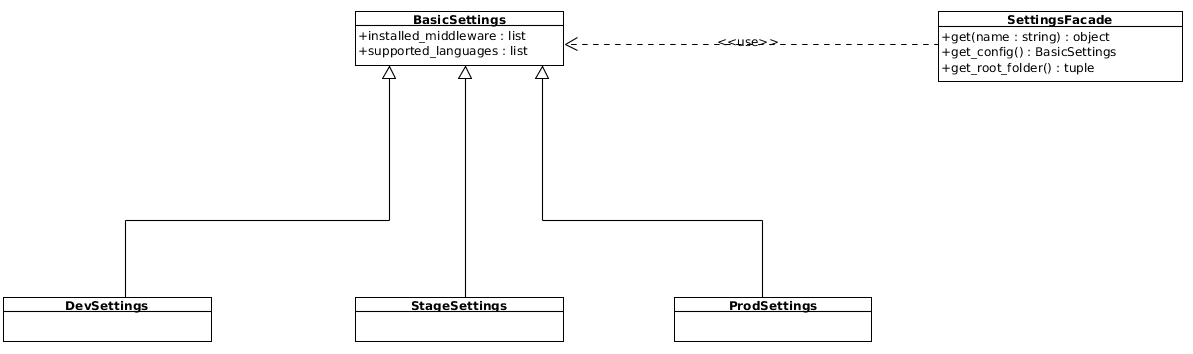
\includegraphics{settings.png}

As you can see, if you want to overwrite basic configuration you simply have to extend the class and set new values
for the attributes you want to overwrite.
\index{access\_token\_validity (fantastico.settings.BasicSettings attribute)}

\begin{fulllineitems}
\phantomsection\label{get_started/settings:fantastico.settings.BasicSettings.access_token_validity}\pysigline{\bfcode{access\_token\_validity}}
This property defines the validity of an access token in seconds. By default, this property is set
to 1h = 3600 seconds.

\end{fulllineitems}

\index{database\_config (fantastico.settings.BasicSettings attribute)}

\begin{fulllineitems}
\phantomsection\label{get_started/settings:fantastico.settings.BasicSettings.database_config}\pysigline{\bfcode{database\_config}}
This property holds the configuration of database. It is recommended to have all environment configured the same.
An exception can be done for host but the rest must remain the same. Below you can find an example of functional
configuration:

\begin{Verbatim}[commandchars=\\\{\}]
\PYG{n}{config} \PYG{o}{=} \PYG{p}{\PYGZob{}}\PYG{l+s}{\PYGZdq{}}\PYG{l+s}{drivername}\PYG{l+s}{\PYGZdq{}}\PYG{p}{:} \PYG{l+s}{\PYGZdq{}}\PYG{l+s}{mysql+mysqlconnector}\PYG{l+s}{\PYGZdq{}}\PYG{p}{,}
            \PYG{l+s}{\PYGZdq{}}\PYG{l+s}{username}\PYG{l+s}{\PYGZdq{}}\PYG{p}{:} \PYG{l+s}{\PYGZdq{}}\PYG{l+s}{fantastico}\PYG{l+s}{\PYGZdq{}}\PYG{p}{,}
            \PYG{l+s}{\PYGZdq{}}\PYG{l+s}{password}\PYG{l+s}{\PYGZdq{}}\PYG{p}{:} \PYG{l+s}{\PYGZdq{}}\PYG{l+s}{12345}\PYG{l+s}{\PYGZdq{}}\PYG{p}{,}
            \PYG{l+s}{\PYGZdq{}}\PYG{l+s}{port}\PYG{l+s}{\PYGZdq{}}\PYG{p}{:} \PYG{l+m+mi}{3306}\PYG{p}{,}
            \PYG{l+s}{\PYGZdq{}}\PYG{l+s}{host}\PYG{l+s}{\PYGZdq{}}\PYG{p}{:} \PYG{l+s}{\PYGZdq{}}\PYG{l+s}{localhost}\PYG{l+s}{\PYGZdq{}}\PYG{p}{,}
            \PYG{l+s}{\PYGZdq{}}\PYG{l+s}{database}\PYG{l+s}{\PYGZdq{}}\PYG{p}{:} \PYG{l+s}{\PYGZdq{}}\PYG{l+s}{fantastico}\PYG{l+s}{\PYGZdq{}}\PYG{p}{,}
            \PYG{l+s}{\PYGZdq{}}\PYG{l+s}{additional\PYGZus{}params}\PYG{l+s}{\PYGZdq{}}\PYG{p}{:} \PYG{p}{\PYGZob{}}\PYG{l+s}{\PYGZdq{}}\PYG{l+s}{charset}\PYG{l+s}{\PYGZdq{}}\PYG{p}{:} \PYG{l+s}{\PYGZdq{}}\PYG{l+s}{utf8}\PYG{l+s}{\PYGZdq{}}\PYG{p}{\PYGZcb{}}\PYG{p}{,}
            \PYG{l+s}{\PYGZdq{}}\PYG{l+s}{show\PYGZus{}sql}\PYG{l+s}{\PYGZdq{}}\PYG{p}{:} \PYG{n+nb+bp}{True}\PYG{p}{,}
            \PYG{l+s}{\PYGZdq{}}\PYG{l+s}{additional\PYGZus{}engine\PYGZus{}settings}\PYG{l+s}{\PYGZdq{}}\PYG{p}{:} \PYG{p}{\PYGZob{}}
                \PYG{l+s}{\PYGZdq{}}\PYG{l+s}{pool\PYGZus{}size}\PYG{l+s}{\PYGZdq{}}\PYG{p}{:} \PYG{l+m+mi}{20}\PYG{p}{,}
                \PYG{l+s}{\PYGZdq{}}\PYG{l+s}{pool\PYGZus{}recycle}\PYG{l+s}{\PYGZdq{}}\PYG{p}{:} \PYG{l+m+mi}{600}\PYG{p}{\PYGZcb{}}
          \PYG{p}{\PYGZcb{}}
\end{Verbatim}

As you can see, in your configuration you can influence many attributes used when configuring the driver / database.
\textbf{show\_sql} key tells orm engine from \textbf{Fantastico} to display all generated queries.

Moreover, by default \textbf{Fantastico} holds connections opened for 10 minutes. After 10 minutes it refreshes the connection
and ensures no thread is using that connection till is completely refreshed.

\end{fulllineitems}

\index{dev\_server\_host (fantastico.settings.BasicSettings attribute)}

\begin{fulllineitems}
\phantomsection\label{get_started/settings:fantastico.settings.BasicSettings.dev_server_host}\pysigline{\bfcode{dev\_server\_host}}
This property holds development server hostname. By default this is localhost.

\end{fulllineitems}

\index{dev\_server\_port (fantastico.settings.BasicSettings attribute)}

\begin{fulllineitems}
\phantomsection\label{get_started/settings:fantastico.settings.BasicSettings.dev_server_port}\pysigline{\bfcode{dev\_server\_port}}
This property holds development server port. By default this is 12000.

\end{fulllineitems}

\index{doc\_base (fantastico.settings.BasicSettings attribute)}

\begin{fulllineitems}
\phantomsection\label{get_started/settings:fantastico.settings.BasicSettings.doc_base}\pysigline{\bfcode{doc\_base}}
This property defines public location of \textbf{Fantastico} documentation.

\end{fulllineitems}

\index{global\_response\_headers (fantastico.settings.BasicSettings attribute)}

\begin{fulllineitems}
\phantomsection\label{get_started/settings:fantastico.settings.BasicSettings.global_response_headers}\pysigline{\bfcode{global\_response\_headers}}
This property defines the headers which must be appended to every response. You can use this property in order
to globally enable cors.

\begin{Verbatim}[commandchars=\\\{\}]
\PYG{k}{return} \PYG{p}{\PYGZob{}}\PYG{l+s}{\PYGZdq{}}\PYG{l+s}{Access\PYGZhy{}Control\PYGZhy{}Allow\PYGZhy{}Origin}\PYG{l+s}{\PYGZdq{}}\PYG{p}{:} \PYG{l+s}{\PYGZdq{}}\PYG{l+s}{*}\PYG{l+s}{\PYGZdq{}}\PYG{p}{\PYGZcb{}}
\end{Verbatim}

By default, no global header is appended to response.

\end{fulllineitems}

\index{installed\_middleware (fantastico.settings.BasicSettings attribute)}

\begin{fulllineitems}
\phantomsection\label{get_started/settings:fantastico.settings.BasicSettings.installed_middleware}\pysigline{\bfcode{installed\_middleware}}
Property that holds all installed middlewares.

\end{fulllineitems}

\index{mvc\_additional\_paths (fantastico.settings.BasicSettings attribute)}

\begin{fulllineitems}
\phantomsection\label{get_started/settings:fantastico.settings.BasicSettings.mvc_additional_paths}\pysigline{\bfcode{mvc\_additional\_paths}}
This property defines additional packages which must be scanned for controllers. You can use this in order to specify
custom mvc controllers location which are not found in custom components. For instance, OAuth2 controller resides
in core packages of Fantastico.

\end{fulllineitems}

\index{oauth2\_idp (fantastico.settings.BasicSettings attribute)}

\begin{fulllineitems}
\phantomsection\label{get_started/settings:fantastico.settings.BasicSettings.oauth2_idp}\pysigline{\bfcode{oauth2\_idp}}
This property holds the configuration for Fantastico default Identity Provider. In most cases you will change the
template applied to login screen in order to customize it to your needs. If you want to change
the template for login screen make sure your provide relative path to your components root folder
(e.g /components/frontend/views/custom\_login.html). Moreover, you can also specify the login token validity period (in
seconds). It is recommended to set a high value (e.g 2 weeks).

Additionaly, you can control default idp index page. Usually, Fantastico OAuth2 identity provider login page should be
good enough.

\begin{Verbatim}[commandchars=\\\{\}]
\PYG{k}{return} \PYG{p}{\PYGZob{}}\PYG{l+s}{\PYGZdq{}}\PYG{l+s}{client\PYGZus{}id}\PYG{l+s}{\PYGZdq{}}\PYG{p}{:} \PYG{l+s}{\PYGZdq{}}\PYG{l+s}{11111111\PYGZhy{}1111\PYGZhy{}1111\PYGZhy{}1111\PYGZhy{}111111111111}\PYG{l+s}{\PYGZdq{}}\PYG{p}{,}
        \PYG{l+s}{\PYGZdq{}}\PYG{l+s}{template}\PYG{l+s}{\PYGZdq{}}\PYG{p}{:} \PYG{l+s}{\PYGZdq{}}\PYG{l+s}{/components/frontend/views/custom\PYGZus{}login.html}\PYG{l+s}{\PYGZdq{}}\PYG{p}{,}
        \PYG{l+s}{\PYGZdq{}}\PYG{l+s}{expires\PYGZus{}in}\PYG{l+s}{\PYGZdq{}}\PYG{p}{:} \PYG{l+m+mi}{1209600}\PYG{p}{,}
        \PYG{l+s}{\PYGZdq{}}\PYG{l+s}{idp\PYGZus{}index}\PYG{l+s}{\PYGZdq{}}\PYG{p}{:} \PYG{l+s}{\PYGZdq{}}\PYG{l+s}{/oauth/idp/ui/login}\PYG{l+s}{\PYGZdq{}}\PYG{p}{\PYGZcb{}}
\end{Verbatim}

\end{fulllineitems}

\index{roa\_api (fantastico.settings.BasicSettings attribute)}

\begin{fulllineitems}
\phantomsection\label{get_started/settings:fantastico.settings.BasicSettings.roa_api}\pysigline{\bfcode{roa\_api}}
This property defines the url for mapping ROA resources api. By default is \textbf{/api}. Read more about ROA on
{\hyperref[features/components/roa_discovery/roa_discovery::doc]{\emph{ROA Auto discovery}}}.

\end{fulllineitems}

\index{routes\_loaders (fantastico.settings.BasicSettings attribute)}

\begin{fulllineitems}
\phantomsection\label{get_started/settings:fantastico.settings.BasicSettings.routes_loaders}\pysigline{\bfcode{routes\_loaders}}
This property holds all routes loaders available.

\end{fulllineitems}

\index{supported\_languages (fantastico.settings.BasicSettings attribute)}

\begin{fulllineitems}
\phantomsection\label{get_started/settings:fantastico.settings.BasicSettings.supported_languages}\pysigline{\bfcode{supported\_languages}}
Property that holds all supported languages by this fantastico instance.

\end{fulllineitems}

\index{templates\_config (fantastico.settings.BasicSettings attribute)}

\begin{fulllineitems}
\phantomsection\label{get_started/settings:fantastico.settings.BasicSettings.templates_config}\pysigline{\bfcode{templates\_config}}
This property holds configuration of templates rendering engine. For the moment this influence how
\href{http://jinja.pocoo.org/docs/}{Jinja2} acts.

\end{fulllineitems}


\end{fulllineitems}



\subsection{Create Dev configuration}
\label{get_started/settings:create-dev-configuration}
Let's imagine you want to create a custom dev configuration for your project. Below you can find the code for this:

\begin{Verbatim}[commandchars=\\\{\}]
\PYG{k}{class} \PYG{n+nc}{DevSettings}\PYG{p}{(}\PYG{n}{BasicSettings}\PYG{p}{)}\PYG{p}{:}
   \PYG{n+nd}{@property}
   \PYG{k}{def} \PYG{n+nf}{supported\PYGZus{}languages}\PYG{p}{(}\PYG{n+nb+bp}{self}\PYG{p}{)}\PYG{p}{:}
      \PYG{k}{return} \PYG{p}{[}\PYG{l+s}{\PYGZdq{}}\PYG{l+s}{en\PYGZus{}us}\PYG{l+s}{\PYGZdq{}}\PYG{p}{,} \PYG{l+s}{\PYGZdq{}}\PYG{l+s}{ro\PYGZus{}ro}\PYG{l+s}{\PYGZdq{}}\PYG{p}{]}
\end{Verbatim}

The above configuration actually overwrites supported languages. This mean that only en\_us is relevant for \textbf{Dev} environment.
You can do the same for \textbf{Stage}, \textbf{Prod} or any other custom configuration.


\subsection{Using a specifc configuration}
\label{get_started/settings:using-a-specifc-configuration}\index{SettingsFacade (class in fantastico.settings)}

\begin{fulllineitems}
\phantomsection\label{get_started/settings:fantastico.settings.SettingsFacade}\pysiglinewithargsret{\strong{class }\code{fantastico.settings.}\bfcode{SettingsFacade}}{\emph{environ=None}}{}
For using a specific fantastico configuration you need to do two simple steps:
\begin{itemize}
\item {} 
Set \textbf{FANTASTICO\_ACTIVE\_CONFIG} environment variable to the fully python qualified class name you want to use. E.g: {\hyperref[get_started/settings:fantastico.settings.BasicSettings]{\code{fantastico.settings.BasicSettings}}}

\item {} 
In your code, you can use the following snippet to access a specific setting:

\begin{Verbatim}[commandchars=\\\{\}]
\PYG{k+kn}{from} \PYG{n+nn}{fantastico.settings} \PYG{k+kn}{import} \PYG{n}{SettingsFacade}

\PYG{k}{print}\PYG{p}{(}\PYG{n}{SettingsFacade}\PYG{p}{(}\PYG{p}{)}\PYG{o}{.}\PYG{n}{get}\PYG{p}{(}\PYG{l+s}{\PYGZdq{}}\PYG{l+s}{installed\PYGZus{}middleware}\PYG{l+s}{\PYGZdq{}}\PYG{p}{)}\PYG{p}{)}
\end{Verbatim}

\end{itemize}

If no active configuration is set in the {\hyperref[get_started/settings:fantastico.settings.BasicSettings]{\code{fantastico.settings.BasicSettings}}} will be used.
\index{get() (fantastico.settings.SettingsFacade method)}

\begin{fulllineitems}
\phantomsection\label{get_started/settings:fantastico.settings.SettingsFacade.get}\pysiglinewithargsret{\bfcode{get}}{\emph{name}}{}
Method used to retrieve a setting value.
\begin{quote}\begin{description}
\item[{Parameters}] \leavevmode\begin{itemize}
\item {} 
\textbf{name} -- Setting name.

\item {} 
\textbf{type} -- string

\end{itemize}

\item[{Returns}] \leavevmode
The setting value.

\item[{Return type}] \leavevmode
object

\end{description}\end{quote}

\end{fulllineitems}

\index{get\_config() (fantastico.settings.SettingsFacade method)}

\begin{fulllineitems}
\phantomsection\label{get_started/settings:fantastico.settings.SettingsFacade.get_config}\pysiglinewithargsret{\bfcode{get\_config}}{}{}
Method used to return the active configuration which is used by this facade.
\begin{quote}\begin{description}
\item[{Return type}] \leavevmode
{\hyperref[get_started/settings:fantastico.settings.BasicSettings]{\code{fantastico.settings.BasicSettings}}}

\item[{Returns}] \leavevmode
Active configuration currently used.

\end{description}\end{quote}

\end{fulllineitems}

\index{get\_root\_folder() (fantastico.settings.SettingsFacade method)}

\begin{fulllineitems}
\phantomsection\label{get_started/settings:fantastico.settings.SettingsFacade.get_root_folder}\pysiglinewithargsret{\bfcode{get\_root\_folder}}{}{}
Method used to return the root folder of the current fantastico project (detected starting from settings)
profile used.

\end{fulllineitems}


\end{fulllineitems}



\section{Contribute}
\label{get_started/contribute:contribute}\label{get_started/contribute::doc}
Fantastico framework is open source so every contribution is welcome. For the moment we are looking for more developers willing to
contribute.


\subsection{Code contribution}
\label{get_started/contribute:code-contribution}
If you want to contribute with code to fantastico framework there are a simple set of rules that you must follow:
\begin{itemize}
\item {} 
Write unit tests (for the code / feature you are contributing).

\item {} 
Write integration tests (for the code / feature you are contributing).

\item {} 
Make sure your code is rated above 9.5 by pylint tool.

\item {} 
In addition integration tests and unit tests must cover 95\% of your code.

\end{itemize}

In order for each build to remain stable the following hard limits are imposed:
\begin{enumerate}
\item {} 
Unit tests must cover \textgreater{}= 95\% of the code.

\item {} 
Integration tests must cover \textgreater{}= 95\% of the code.

\item {} 
Code must be rated above 9.5 by pylint.

\item {} 
Everything must pass.

\end{enumerate}

When you push on master a set of jobs are cascaded executed:
\begin{enumerate}
\item {} 
Run all unit tests job.

\item {} 
Run all integration tests job (only if unit tests succeeds).

\item {} 
Generate documentation and publish it (only if integration tests job succeeds).

\end{enumerate}

You can follow the above build process by visiting
\href{http://jenkins.scrum-expert.ro:8080/job/fantastico-framework/}{Jenkins build}. Login with your github account and everything
should work smoothly.

In the end do not forget that in Fantastico framework we love to develop against a \textbf{stable} base. We really think code will have
high quality and zero bugs.


\subsubsection{Writing unit tests}
\label{get_started/contribute:writing-unit-tests}
For better understanding how to write unit tests see the documentation below:
\index{FantasticoUnitTestsCase (class in fantastico.tests.base\_case)}

\begin{fulllineitems}
\phantomsection\label{get_started/contribute:fantastico.tests.base_case.FantasticoUnitTestsCase}\pysiglinewithargsret{\strong{class }\code{fantastico.tests.base\_case.}\bfcode{FantasticoUnitTestsCase}}{\emph{methodName='runTest'}}{}
This is the base class that must be inherited by each unit test written for fantastico.

\begin{Verbatim}[commandchars=\\\{\}]
\PYG{k}{class} \PYG{n+nc}{SimpleUnitTest}\PYG{p}{(}\PYG{n}{FantasticoUnitTestsCase}\PYG{p}{)}\PYG{p}{:}
    \PYG{k}{def} \PYG{n+nf}{init}\PYG{p}{(}\PYG{n+nb+bp}{self}\PYG{p}{)}\PYG{p}{:}
        \PYG{n+nb+bp}{self}\PYG{o}{.}\PYG{n}{\PYGZus{}msg} \PYG{o}{=} \PYG{l+s}{\PYGZdq{}}\PYG{l+s}{Hello world}\PYG{l+s}{\PYGZdq{}}

    \PYG{k}{def} \PYG{n+nf}{test\PYGZus{}simple\PYGZus{}flow\PYGZus{}ok}\PYG{p}{(}\PYG{n+nb+bp}{self}\PYG{p}{)}\PYG{p}{:}
        \PYG{n+nb+bp}{self}\PYG{o}{.}\PYG{n}{assertEqual}\PYG{p}{(}\PYG{l+s}{\PYGZdq{}}\PYG{l+s}{Hello world}\PYG{l+s}{\PYGZdq{}}\PYG{p}{,} \PYG{n+nb+bp}{self}\PYG{o}{.}\PYG{n}{\PYGZus{}msg}\PYG{p}{)}
\end{Verbatim}
\index{\_get\_class\_root\_folder() (fantastico.tests.base\_case.FantasticoUnitTestsCase method)}

\begin{fulllineitems}
\phantomsection\label{get_started/contribute:fantastico.tests.base_case.FantasticoUnitTestsCase._get_class_root_folder}\pysiglinewithargsret{\bfcode{\_get\_class\_root\_folder}}{}{}
This methods determines the root folder under which the test is executed.

\end{fulllineitems}

\index{\_get\_root\_folder() (fantastico.tests.base\_case.FantasticoUnitTestsCase method)}

\begin{fulllineitems}
\phantomsection\label{get_started/contribute:fantastico.tests.base_case.FantasticoUnitTestsCase._get_root_folder}\pysiglinewithargsret{\bfcode{\_get\_root\_folder}}{}{}
This method determines the root folder under which core is executed.

\end{fulllineitems}

\index{check\_original\_methods() (fantastico.tests.base\_case.FantasticoUnitTestsCase method)}

\begin{fulllineitems}
\phantomsection\label{get_started/contribute:fantastico.tests.base_case.FantasticoUnitTestsCase.check_original_methods}\pysiglinewithargsret{\bfcode{check\_original\_methods}}{\emph{cls\_obj}}{}
This method ensures that for a given class only original non decorated methods will be invoked. Extremely useful
when you want to make sure @Controller decorator does not break your tests. It is strongly recommended to invoke
this method on all classes which might contain @Controller decorator. It ease your when committing on CI environment.

\end{fulllineitems}

\index{setup\_once() (fantastico.tests.base\_case.FantasticoUnitTestsCase class method)}

\begin{fulllineitems}
\phantomsection\label{get_started/contribute:fantastico.tests.base_case.FantasticoUnitTestsCase.setup_once}\pysiglinewithargsret{\strong{classmethod }\bfcode{setup\_once}}{}{}
This method is overriden in order to correctly mock some dependencies:
\begin{itemize}
\item {} 
{\hyperref[features/mvc:fantastico.mvc.controller_decorators.Controller]{\code{fantastico.mvc.controller\_decorators.Controller}}}

\end{itemize}

\end{fulllineitems}


\end{fulllineitems}



\subsubsection{Writing integration tests}
\label{get_started/contribute:writing-integration-tests}
For better understanding how to write integration tests see the documentation below:
\index{FantasticoIntegrationTestCase (class in fantastico.tests.base\_case)}

\begin{fulllineitems}
\phantomsection\label{get_started/contribute:fantastico.tests.base_case.FantasticoIntegrationTestCase}\pysiglinewithargsret{\strong{class }\code{fantastico.tests.base\_case.}\bfcode{FantasticoIntegrationTestCase}}{\emph{methodName='runTest'}}{}
This is the base class that must be inherited by each integration test written for fantastico.
If you used this class you don't have to mind about restoring call methods from each middleware once they are wrapped
by fantastico app. This is a must because otherwise you will crash other tests.
\index{\_envs (fantastico.tests.base\_case.FantasticoIntegrationTestCase attribute)}

\begin{fulllineitems}
\phantomsection\label{get_started/contribute:fantastico.tests.base_case.FantasticoIntegrationTestCase._envs}\pysigline{\bfcode{\_envs}}
Private property that holds the environments against which we run the integration tests.

\end{fulllineitems}

\index{\_get\_db\_conn() (fantastico.tests.base\_case.FantasticoIntegrationTestCase method)}

\begin{fulllineitems}
\phantomsection\label{get_started/contribute:fantastico.tests.base_case.FantasticoIntegrationTestCase._get_db_conn}\pysiglinewithargsret{\bfcode{\_get\_db\_conn}}{}{}
This method opens a db connection and returns it to for usage.

\end{fulllineitems}

\index{\_get\_oauth2\_logintoken() (fantastico.tests.base\_case.FantasticoIntegrationTestCase method)}

\begin{fulllineitems}
\phantomsection\label{get_started/contribute:fantastico.tests.base_case.FantasticoIntegrationTestCase._get_oauth2_logintoken}\pysiglinewithargsret{\bfcode{\_get\_oauth2\_logintoken}}{\emph{client\_id}, \emph{user\_id}}{}
This methods generates an oauth2 login token which can be used in integration tests.

\end{fulllineitems}

\index{\_get\_oauth2\_token() (fantastico.tests.base\_case.FantasticoIntegrationTestCase method)}

\begin{fulllineitems}
\phantomsection\label{get_started/contribute:fantastico.tests.base_case.FantasticoIntegrationTestCase._get_oauth2_token}\pysiglinewithargsret{\bfcode{\_get\_oauth2\_token}}{\emph{client\_id}, \emph{user\_id}, \emph{scopes}}{}
This method generates an oauth2 access token which can be used in integration tests.

\end{fulllineitems}

\index{\_get\_token() (fantastico.tests.base\_case.FantasticoIntegrationTestCase method)}

\begin{fulllineitems}
\phantomsection\label{get_started/contribute:fantastico.tests.base_case.FantasticoIntegrationTestCase._get_token}\pysiglinewithargsret{\bfcode{\_get\_token}}{\emph{token\_type}, \emph{token\_desc}}{}
This method provides a generic token generation method which can be used in integration tests.

\end{fulllineitems}

\index{\_invalidate\_encrypted\_token() (fantastico.tests.base\_case.FantasticoIntegrationTestCase method)}

\begin{fulllineitems}
\phantomsection\label{get_started/contribute:fantastico.tests.base_case.FantasticoIntegrationTestCase._invalidate_encrypted_token}\pysiglinewithargsret{\bfcode{\_invalidate\_encrypted\_token}}{\emph{encrypted\_token}}{}
This method invalidates a given encrypted token using tokens service implementation.

\end{fulllineitems}

\index{\_invalidate\_oauth2\_token() (fantastico.tests.base\_case.FantasticoIntegrationTestCase method)}

\begin{fulllineitems}
\phantomsection\label{get_started/contribute:fantastico.tests.base_case.FantasticoIntegrationTestCase._invalidate_oauth2_token}\pysiglinewithargsret{\bfcode{\_invalidate\_oauth2\_token}}{\emph{token}}{}
This method invalidates the given token automatically.

\end{fulllineitems}

\index{\_restore\_call\_methods() (fantastico.tests.base\_case.FantasticoIntegrationTestCase method)}

\begin{fulllineitems}
\phantomsection\label{get_started/contribute:fantastico.tests.base_case.FantasticoIntegrationTestCase._restore_call_methods}\pysiglinewithargsret{\bfcode{\_restore\_call\_methods}}{}{}
This method restore original call methods to all affected middlewares.

\end{fulllineitems}

\index{\_save\_call\_methods() (fantastico.tests.base\_case.FantasticoIntegrationTestCase method)}

\begin{fulllineitems}
\phantomsection\label{get_started/contribute:fantastico.tests.base_case.FantasticoIntegrationTestCase._save_call_methods}\pysiglinewithargsret{\bfcode{\_save\_call\_methods}}{\emph{middlewares}}{}
This method save all call methods for each listed middleware so that later on they can be restored.

\end{fulllineitems}

\index{fantastico\_cfg\_os\_key (fantastico.tests.base\_case.FantasticoIntegrationTestCase attribute)}

\begin{fulllineitems}
\phantomsection\label{get_started/contribute:fantastico.tests.base_case.FantasticoIntegrationTestCase.fantastico_cfg_os_key}\pysigline{\bfcode{fantastico\_cfg\_os\_key}}
This property holds the name of os environment variable used for setting up active fantastico configuration.

\end{fulllineitems}


\end{fulllineitems}

\index{DevServerIntegration (class in fantastico.server.tests.itest\_dev\_server)}

\begin{fulllineitems}
\phantomsection\label{get_started/contribute:fantastico.server.tests.itest_dev_server.DevServerIntegration}\pysiglinewithargsret{\strong{class }\code{fantastico.server.tests.itest\_dev\_server.}\bfcode{DevServerIntegration}}{\emph{methodName='runTest'}}{}
This class provides the foundation for writing integration tests that do http requests against a fantastico server.

\begin{Verbatim}[commandchars=\\\{\}]
\PYG{k}{class} \PYG{n+nc}{DummyLoaderIntegration}\PYG{p}{(}\PYG{n}{DevServerIntegration}\PYG{p}{)}\PYG{p}{:}
    \PYG{k}{def} \PYG{n+nf}{init}\PYG{p}{(}\PYG{n+nb+bp}{self}\PYG{p}{)}\PYG{p}{:}
        \PYG{n+nb+bp}{self}\PYG{o}{.}\PYG{n}{\PYGZus{}exception} \PYG{o}{=} \PYG{n+nb+bp}{None}

    \PYG{k}{def} \PYG{n+nf}{test\PYGZus{}server\PYGZus{}runs\PYGZus{}ok}\PYG{p}{(}\PYG{n+nb+bp}{self}\PYG{p}{)}\PYG{p}{:}
        \PYG{k}{def} \PYG{n+nf}{request\PYGZus{}logic}\PYG{p}{(}\PYG{n}{server}\PYG{p}{)}\PYG{p}{:}
            \PYG{n}{request} \PYG{o}{=} \PYG{n}{Request}\PYG{p}{(}\PYG{n+nb+bp}{self}\PYG{o}{.}\PYG{n}{\PYGZus{}get\PYGZus{}server\PYGZus{}base\PYGZus{}url}\PYG{p}{(}\PYG{n}{server}\PYG{p}{,} \PYG{n}{DummyRouteLoader}\PYG{o}{.}\PYG{n}{DUMMY\PYGZus{}ROUTE}\PYG{p}{)}\PYG{p}{)}
            \PYG{k}{with} \PYG{n+nb+bp}{self}\PYG{o}{.}\PYG{n}{assertRaises}\PYG{p}{(}\PYG{n}{HTTPError}\PYG{p}{)} \PYG{k}{as} \PYG{n}{cm}\PYG{p}{:}
                \PYG{n}{urllib}\PYG{o}{.}\PYG{n}{request}\PYG{o}{.}\PYG{n}{urlopen}\PYG{p}{(}\PYG{n}{request}\PYG{p}{)}

            \PYG{n+nb+bp}{self}\PYG{o}{.}\PYG{n}{\PYGZus{}exception} \PYG{o}{=} \PYG{n}{cm}\PYG{o}{.}\PYG{n}{exception}

        \PYG{k}{def} \PYG{n+nf}{assert\PYGZus{}logic}\PYG{p}{(}\PYG{n}{server}\PYG{p}{)}\PYG{p}{:}
            \PYG{n+nb+bp}{self}\PYG{o}{.}\PYG{n}{assertEqual}\PYG{p}{(}\PYG{l+m+mi}{400}\PYG{p}{,} \PYG{n+nb+bp}{self}\PYG{o}{.}\PYG{n}{\PYGZus{}exception}\PYG{o}{.}\PYG{n}{code}\PYG{p}{)}
            \PYG{n+nb+bp}{self}\PYG{o}{.}\PYG{n}{assertEqual}\PYG{p}{(}\PYG{l+s}{\PYGZdq{}}\PYG{l+s}{Hello world.}\PYG{l+s}{\PYGZdq{}}\PYG{p}{,} \PYG{n+nb+bp}{self}\PYG{o}{.}\PYG{n}{\PYGZus{}exception}\PYG{o}{.}\PYG{n}{read}\PYG{p}{(}\PYG{p}{)}\PYG{o}{.}\PYG{n}{decode}\PYG{p}{(}\PYG{p}{)}\PYG{p}{)}

        \PYG{n+nb+bp}{self}\PYG{o}{.}\PYG{n}{\PYGZus{}run\PYGZus{}test\PYGZus{}against\PYGZus{}dev\PYGZus{}server}\PYG{p}{(}\PYG{n}{request\PYGZus{}logic}\PYG{p}{,} \PYG{n}{assert\PYGZus{}logic}\PYG{p}{)}
\end{Verbatim}

As you can see from above listed code, when you write a new integration test against Fantastico server you only need
to provide the request logic and assert logic functions. Request logic is executed while the server is up and running.
Assert logic is executed after the server has stopped.
\index{\_check\_server\_started() (fantastico.server.tests.itest\_dev\_server.DevServerIntegration method)}

\begin{fulllineitems}
\phantomsection\label{get_started/contribute:fantastico.server.tests.itest_dev_server.DevServerIntegration._check_server_started}\pysiglinewithargsret{\bfcode{\_check\_server\_started}}{\emph{server}}{}
This method holds the sanity checks to ensure a server is started correctly.

\end{fulllineitems}

\index{\_get\_server\_base\_url() (fantastico.server.tests.itest\_dev\_server.DevServerIntegration method)}

\begin{fulllineitems}
\phantomsection\label{get_started/contribute:fantastico.server.tests.itest_dev_server.DevServerIntegration._get_server_base_url}\pysiglinewithargsret{\bfcode{\_get\_server\_base\_url}}{\emph{server}, \emph{route}}{}
This method returns the absolute url for a given relative url (route).

\end{fulllineitems}

\index{\_run\_test\_against\_dev\_server() (fantastico.server.tests.itest\_dev\_server.DevServerIntegration method)}

\begin{fulllineitems}
\phantomsection\label{get_started/contribute:fantastico.server.tests.itest_dev_server.DevServerIntegration._run_test_against_dev_server}\pysiglinewithargsret{\bfcode{\_run\_test\_against\_dev\_server}}{\emph{request\_logic}, \emph{assert\_logic=None}}{}
This method provides a template for writing integration tests that requires a development server being active.
It accepts a request logic (code that actually do the http request) and an assert logic for making sure
code is correct.

\end{fulllineitems}


\end{fulllineitems}



\section{Development mode}
\label{get_started/dev_mode::doc}\label{get_started/dev_mode:development-mode}
\textbf{Fantastico} framework is a web framework designed to be developers friendly. In order to simplify setup sequence, fantastico
provides a standalone WSGI compatible server that can be started from command line. This server is fully compliant with WSGI
standard. Below you can find some easy steps to achieve this:
\begin{enumerate}
\item {} 
Goto fantastico framework or project location

\item {} 
sh run\_dev\_server.sh

\end{enumerate}

This is it. Now you have a running fantastico server on which you can test your work.

By default, \textbf{Fantastico} dev server starts on port 12000, but you can customize it from
{\hyperref[get_started/settings:fantastico.settings.BasicSettings]{\code{fantastico.settings.BasicSettings}}}.


\subsection{Hot deploy}
\label{get_started/dev_mode:hot-deploy}
Currently, this is not implemented, but it is on todo list on short term.


\subsection{API}
\label{get_started/dev_mode:api}
For more information about Fantastico development server see the API below.
\index{DevServer (class in fantastico.server.dev\_server)}

\begin{fulllineitems}
\phantomsection\label{get_started/dev_mode:fantastico.server.dev_server.DevServer}\pysiglinewithargsret{\strong{class }\code{fantastico.server.dev\_server.}\bfcode{DevServer}}{\emph{settings\_facade=\textless{}class `fantastico.settings.SettingsFacade'\textgreater{}}}{}
This class provides a very simple wsgi http server that embeds Fantastico framework into it. As developer you can use
it to simply test your new components.
\index{start() (fantastico.server.dev\_server.DevServer method)}

\begin{fulllineitems}
\phantomsection\label{get_started/dev_mode:fantastico.server.dev_server.DevServer.start}\pysiglinewithargsret{\bfcode{start}}{\emph{build\_server=\textless{}function make\_server at 0x54caa68\textgreater{}}, \emph{app=\textless{}class `fantastico.middleware.fantastico\_app.FantasticoApp'\textgreater{}}}{}
This method starts a WSGI development server. All attributes like port, hostname and protocol are read from
configuration file.

\end{fulllineitems}

\index{started (fantastico.server.dev\_server.DevServer attribute)}

\begin{fulllineitems}
\phantomsection\label{get_started/dev_mode:fantastico.server.dev_server.DevServer.started}\pysigline{\bfcode{started}}
Property used to tell if development server is started or not.

\end{fulllineitems}

\index{stop() (fantastico.server.dev\_server.DevServer method)}

\begin{fulllineitems}
\phantomsection\label{get_started/dev_mode:fantastico.server.dev_server.DevServer.stop}\pysiglinewithargsret{\bfcode{stop}}{}{}
This method stops the current running server (if any available).

\end{fulllineitems}


\end{fulllineitems}



\subsection{Database config}
\label{get_started/dev_mode:database-config}
Usually you will use \textbf{Fantastico} framework together with a database. When we develop new core features of \textbf{Fantastico}
we use a sample database for integration. You can easily use it as well to play around:
\begin{enumerate}
\item {} 
Goto fantastico framework location

\item {} 
export MYSQL\_PASSWD=***** (your mysql password)

\item {} 
export MYSQL\_HOST=\textless{}hostname\textgreater{} (your mysql hostname: e.g localhost)

\item {} 
sh run\_setup\_db.sh

\end{enumerate}

\textbf{run\_setup\_db.sh} create an initial fantastico database and a user called fantastico identified by \textbf{12345} password. After
database is successfully created, it scans for all available \textbf{module\_setup.sql} files and execute them against newly created
database.


\chapter{How to articles}
\label{how_to/how_to:how-to-articles}\label{how_to/how_to::doc}

\section{Creating a new project}
\label{how_to/new_project_how_to:creating-a-new-project}\label{how_to/new_project_how_to::doc}
A new Fantastico based project can be easily setup by following this how to. In this how to we are going to create
a project named \textbf{fantastico\_first}.
\begin{enumerate}
\item {} 
cd \textasciitilde{}/

\item {} 
mkdir fantastico\_first

\item {} 
cd fantastico\_first

\item {} 
virtualenv-3.2 --distribute pip-deps

\item {} 
. pip-deps/bin/activate

\item {} 
pip install fantastico

\item {} 
fantastico\_setup\_project.sh python3.2 my\_project

\end{enumerate}

The last step might take a while because it will also install all fantastico dependencies (e.g sphinx, sqlalchemy, ...).
Please make sure your replace python3.2 with the correct python version.
In order to test the current project do the following:
\begin{enumerate}
\item {} 
fantastico\_run\_dev\_server

\item {} 
Access \href{http://localhost:12000/mvc/hello-world}{http://localhost:12000/mvc/hello-world}

\end{enumerate}

Your newly project is setup correctly and it runs fantastico default samples project.


\subsection{Create first component}
\label{how_to/new_project_how_to:create-first-component}
After the new project it's correctly setup we can create our first component.
\begin{enumerate}
\item {} 
. pip-deps/bin/activate

\item {} 
export FANTASTICO\_ACTIVE\_CONFIG=my\_project.settings.BaseProfile

\item {} 
cd my\_project

\item {} 
mkdir component1

\item {} 
cd component1

\item {} 
mkdir static

\item {} 
Paste an image into static folder (e.g first\_photo.jpg)

\item {} 
touch \_\_init\_\_.py

\item {} 
touch hello\_world.py

\item {} 
Paste the code listed below into hello\_world.py

\begin{Verbatim}[commandchars=\\\{\}]
\PYG{k+kn}{from} \PYG{n+nn}{fantastico.mvc.base\PYGZus{}controller} \PYG{k+kn}{import} \PYG{n}{BaseController}
\PYG{k+kn}{from} \PYG{n+nn}{fantastico.mvc.controller\PYGZus{}decorators} \PYG{k+kn}{import} \PYG{n}{ControllerProvider}\PYG{p}{,} \PYG{n}{Controller}
\PYG{k+kn}{from} \PYG{n+nn}{webob.response} \PYG{k+kn}{import} \PYG{n}{Response}

\PYG{n+nd}{@ControllerProvider}\PYG{p}{(}\PYG{p}{)}
\PYG{k}{class} \PYG{n+nc}{HelloWorldController}\PYG{p}{(}\PYG{n}{BaseController}\PYG{p}{)}\PYG{p}{:}
    \PYG{l+s+sd}{\PYGZsq{}\PYGZsq{}\PYGZsq{}This is a very simple controller provider.\PYGZsq{}\PYGZsq{}\PYGZsq{}}

    \PYG{n+nd}{@Controller}\PYG{p}{(}\PYG{n}{url}\PYG{o}{=}\PYG{l+s}{\PYGZdq{}}\PYG{l+s}{/component1/hello}\PYG{l+s}{\PYGZdq{}}\PYG{p}{)}
    \PYG{k}{def} \PYG{n+nf}{say\PYGZus{}hello}\PYG{p}{(}\PYG{n+nb+bp}{self}\PYG{p}{,} \PYG{n}{request}\PYG{p}{)}\PYG{p}{:}
        \PYG{l+s+sd}{\PYGZsq{}\PYGZsq{}\PYGZsq{}This method simply returns an html hello world text.\PYGZsq{}\PYGZsq{}\PYGZsq{}}

        \PYG{n}{msg} \PYG{o}{=} \PYG{l+s}{\PYGZdq{}}\PYG{l+s}{Hello world from my project}\PYG{l+s}{\PYGZdq{}}

        \PYG{k}{return} \PYG{n}{Response}\PYG{p}{(}\PYG{n}{content\PYGZus{}type}\PYG{o}{=}\PYG{l+s}{\PYGZdq{}}\PYG{l+s}{text/html}\PYG{l+s}{\PYGZdq{}}\PYG{p}{,} \PYG{n}{text}\PYG{o}{=}\PYG{n}{msg}\PYG{p}{)}
\end{Verbatim}

\item {} 
fantastico\_dev\_server

\item {} 
Now you can access \href{http://localhost:12000/component1/hello}{Hello route}.

\item {} 
Now you can access \href{http://localhost:12000/component1/static/first\_photo.jpg}{First photo route}.

\end{enumerate}


\subsection{Customize dev server}
\label{how_to/new_project_how_to:customize-dev-server}
For understanding how to customize dev server please read {\hyperref[get_started/dev_mode::doc]{\emph{Development mode}}}


\subsection{Customize uwsgi prod server}
\label{how_to/new_project_how_to:customize-uwsgi-prod-server}
By design, each Fantastico project provides built in support for running it on \href{http://uwsgi-docs.readthedocs.org/en/latest/}{uWSGI server}.
If you want to customize uwsgi parameters for your server you can follow these steps:
\begin{enumerate}
\item {} 
cd \$FANTASTICO\_PROJECT\_FOLDER/deployment/conf/nginx

\item {} 
nano fantastico-uwsgi.ini

\item {} 
Change the options you want and save the file.

\item {} 
fantastico\_run\_prod\_server (for testing the production server).

\item {} 
Be aware that first you need an nginx configured and your project config file deployed (Read {\hyperref[how_to/deployment_how_to::doc]{\emph{Deployment how to}}}).

\end{enumerate}


\section{Creating a simple TODO application}
\label{how_to/todo/index:creating-a-simple-todo-application}\label{how_to/todo/index::doc}
In this how to article you can find information of how you can create a TODO web application using Fantastico framework. This
tutorial works with Fantastico versions greater or equal than \href{http://pypi.python.org/pypi/fantastico/0.5.0}{0.5.0}.


\subsection{Functional requirements}
\label{how_to/todo/index:functional-requirements}
The application we are going to develop must meet the following requirements:
\begin{itemize}
\item {} 
User must be able to create tasks.

\item {} 
User must be able to see all tasks.

\item {} 
User must be able to quickly filter tasks.

\item {} 
User must be able to complete tasks.

\item {} 
User must be able to use an web application for managing tasks.

\end{itemize}


\subsection{Overview}
\label{how_to/todo/index:overview}\begin{figure}[htbp]
\centering
\capstart

\scalebox{1.000000}{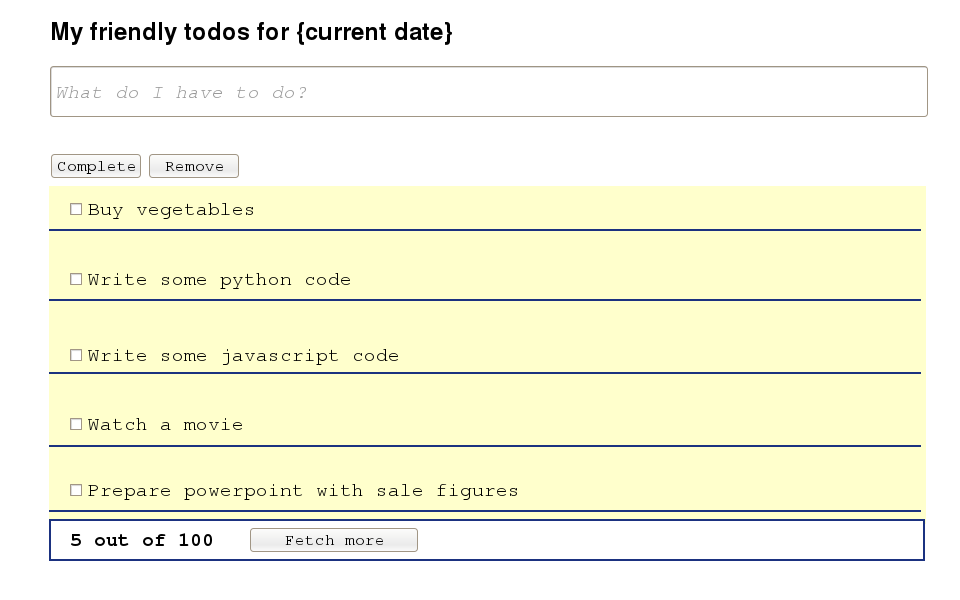
\includegraphics{main_page.png}}
\caption{TODO web application powered by Fantastico.}\end{figure}

The frontend is powered by the following API endpoints:

\begin{tabulary}{\linewidth}{|L|L|L|L|}
\hline

\textbf{Endpoint}
 & 
\textbf{HTTP verb}
 & 
\textbf{HTTP Body}
 & 
\textbf{Description}
\\\hline

/tasks
 & 
GET
 & 
None
 & 
Retrieves available tasks in a paginated manner.
\\\hline

/tasks
 & 
POST
 & 
\{``name'': ``Task name'', ``description'': ``Task description''\}
 & 
Creates a new task described by the given body.
\\\hline

/tasks/:task\_id
 & 
GET
 & 
None
 & 
Retrieves a specific task from tasks collection.
\\\hline

/tasks/:task\_id
 & 
PUT
 & 
\{``name'': ``Task name changed'', ``description'': ``Task description changed''\}
 & 
Updates a specific task from tasks collection.
\\\hline

/tasks/:task\_id
 & 
DELETE
 & 
None
 & 
Deletes a specific task from tasks collection.
\\\hline
\end{tabulary}



\subsection{How to sources}
\label{how_to/todo/index:how-to-sources}
All tutorial source files are available on github: \href{https://github.com/rcosnita/fantastico-todo}{https://github.com/rcosnita/fantastico-todo}. Each step of the tutorial
has a corresponding branch in the github repository so you can easily skip steps of this tutuorial. Though you can skip steps
we recommend you take 30 minutes and finish this step by step how to in order to fully understand the power of Fantastico
framework and how easy it is to build modern web applications using it.


\subsection{Requirements}
\label{how_to/todo/index:requirements}
This tutorial requires developer to have:
\begin{enumerate}
\item {} 
A Debian based operating system

\item {} 
Access to a mysql database.

\item {} 
Python 3.2 or newer.

\end{enumerate}


\subsection{Next steps}
\label{how_to/todo/index:next-steps}

\subsubsection{Step 0 - TODO setup}
\label{how_to/todo/setup::doc}\label{how_to/todo/setup:step-0-todo-setup}
Follow the steps below in order to setup todo web application project correctly:
\begin{enumerate}
\item {} 
git clone \href{https://github.com/rcosnita/fantastico-todo.git}{https://github.com/rcosnita/fantastico-todo.git} fantastico-todo

\item {} 
cd fantastico-todo

\item {} 
virtualenv-3.2 --distribute pip-deps

\item {} 
. pip-deps/bin/activate

\item {} 
pip install fantastico

\item {} 
fantastico\_setup\_project.sh python3.2 todo
* (this will take a couple of minutes because it installs all dependencies).

\end{enumerate}

At this moment you have a \textbf{Fantastico} project created and a component module holder named todo initialized.
For more information about advanced project setup you can always read {\hyperref[how_to/new_project_how_to::doc]{\emph{Creating a new project}}}.


\subsubsection{Step 1 - TODO settings}
\label{how_to/todo/step_1_settings:step-1-todo-settings}\label{how_to/todo/step_1_settings::doc}
In this section of the tutorial you can find information about how to correctly configure database parameters. Follow the steps
below in order to have correct settings for TODO web applications:
\begin{enumerate}
\item {} 
git checkout -b step-1-settings

\item {} 
Paste the code below under fantastico-todo/pip-deps/bin/activate at the end of the file.

\begin{Verbatim}[commandchars=\\\{\}]
\PYG{c}{\PYGZsh{} fantastico\PYGZhy{}todo/pip\PYGZhy{}deps/bin/activate}

\PYG{n+nb}{export }\PYG{n+nv}{FANTASTICO\PYGZus{}ACTIVE\PYGZus{}CONFIG}\PYG{o}{=}todo.settings.BaseProfile
\PYG{n+nb}{export }\PYG{n+nv}{PYTHONPATH}\PYG{o}{=}.
\end{Verbatim}

\item {} 
Paste the code below under fantastico-todo/todo/settings.py

\begin{Verbatim}[commandchars=\\\{\}]
\PYG{c}{\PYGZsh{} fantastico\PYGZhy{}todo/todo/settings.py}

\PYG{k+kn}{from} \PYG{n+nn}{fantastico.settings} \PYG{k+kn}{import} \PYG{n}{BasicSettings}

\PYG{k}{class} \PYG{n+nc}{BaseProfile}\PYG{p}{(}\PYG{n}{BasicSettings}\PYG{p}{)}\PYG{p}{:}
    \PYG{l+s+sd}{\PYGZsq{}\PYGZsq{}\PYGZsq{}todo web application base profile.\PYGZsq{}\PYGZsq{}\PYGZsq{}}

    \PYG{n+nd}{@property}
    \PYG{k}{def} \PYG{n+nf}{database\PYGZus{}config}\PYG{p}{(}\PYG{n+nb+bp}{self}\PYG{p}{)}\PYG{p}{:}
        \PYG{l+s+sd}{\PYGZsq{}\PYGZsq{}\PYGZsq{}This property is automatically invoked by fantastico in order to connect to database.\PYGZsq{}\PYGZsq{}\PYGZsq{}}

        \PYG{n}{db\PYGZus{}config} \PYG{o}{=} \PYG{n+nb}{super}\PYG{p}{(}\PYG{n}{BaseProfile}\PYG{p}{,} \PYG{n+nb+bp}{self}\PYG{p}{)}\PYG{o}{.}\PYG{n}{database\PYGZus{}config}

        \PYG{n}{db\PYGZus{}config}\PYG{p}{[}\PYG{l+s}{\PYGZdq{}}\PYG{l+s}{database}\PYG{l+s}{\PYGZdq{}}\PYG{p}{]} \PYG{o}{=} \PYG{l+s}{\PYGZdq{}}\PYG{l+s}{tododb}\PYG{l+s}{\PYGZdq{}}
        \PYG{n}{db\PYGZus{}config}\PYG{p}{[}\PYG{l+s}{\PYGZdq{}}\PYG{l+s}{username}\PYG{l+s}{\PYGZdq{}}\PYG{p}{]} \PYG{o}{=} \PYG{l+s}{\PYGZdq{}}\PYG{l+s}{todo\PYGZus{}user}\PYG{l+s}{\PYGZdq{}}
        \PYG{n}{db\PYGZus{}config}\PYG{p}{[}\PYG{l+s}{\PYGZdq{}}\PYG{l+s}{password}\PYG{l+s}{\PYGZdq{}}\PYG{p}{]} \PYG{o}{=} \PYG{l+s}{\PYGZdq{}}\PYG{l+s}{12345}\PYG{l+s}{\PYGZdq{}}

        \PYG{k}{return} \PYG{n}{db\PYGZus{}config}
\end{Verbatim}

\item {} 
Run the command below in order to make sure sdk is working:

\begin{Verbatim}[commandchars=\\\{\}]
fsdk \PYGZhy{}\PYGZhy{}help
\end{Verbatim}

You should see a screen similar to the one below:

\scalebox{1.000000}{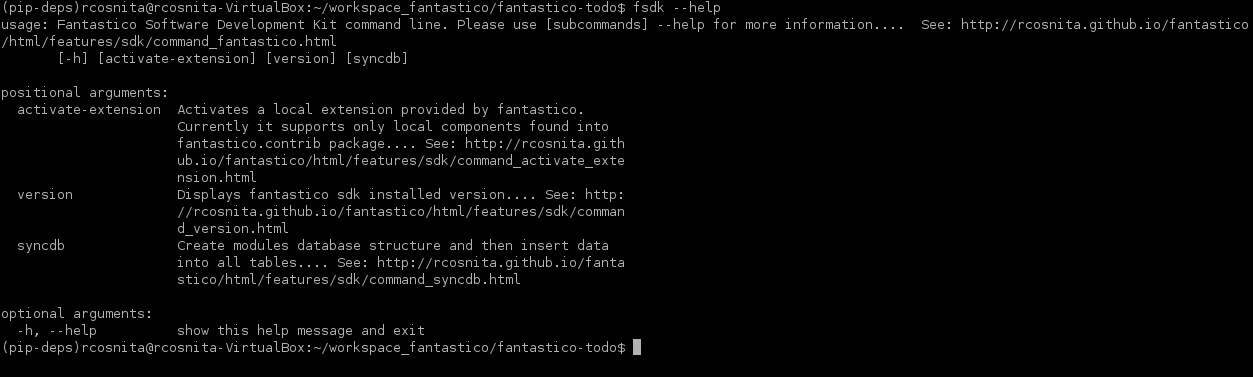
\includegraphics{fsdk_help.png}}

\item {} 
Execute the code below in order to create \textbf{tododb} database.

\begin{Verbatim}[commandchars=\\\{\}]
/usr/bin/mysql \PYGZhy{}\PYGZhy{}host\PYG{o}{=}localhost \PYGZhy{}\PYGZhy{}user\PYG{o}{=}root \PYGZhy{}\PYGZhy{}password\PYG{o}{=}**** \PYGZhy{}\PYGZhy{}verbose \PYGZhy{}e \PYG{l+s+s2}{\PYGZdq{}source sql/setup\PYGZus{}database.sql\PYGZdq{}}
\end{Verbatim}

\end{enumerate}


\paragraph{Explanation}
\label{how_to/todo/step_1_settings:explanation}
We have just configured our virtual development environment for \textbf{TODO} web application to use \textbf{tododb} with
\textbf{todo\_user/12345} credentials. You can of course configure more details of your connection:
\begin{itemize}
\item {} 
MySql host.

\item {} 
MySql port.

\item {} 
MySql charset.

\end{itemize}

For a complete list of database configuration in \textbf{Fantastico framework} please read {\hyperref[get_started/settings::doc]{\emph{Fantastico settings}}}.

In addition, we created a dedicated database for \textbf{TODO} web application.


\subsubsection{Step 2 - TODO API endpoints}
\label{how_to/todo/step_2_create_api:step-2-todo-api-endpoints}\label{how_to/todo/step_2_create_api::doc}
In this section of \textbf{TODO} how to we are going to create the following API endpoints:

\begin{tabulary}{\linewidth}{|L|L|L|L|}
\hline

\textbf{Endpoint}
 & 
\textbf{HTTP verb}
 & 
\textbf{HTTP Body}
 & 
\textbf{Description}
\\\hline

/tasks
 & 
GET
 & 
None
 & 
Retrieves available tasks in a paginated manner.
\\\hline

/tasks
 & 
POST
 & 
\{``name'': ``Task name'', ``description'': ``Task description''\}
 & 
Creates a new task described by the given body.
\\\hline

/tasks/:task\_id
 & 
GET
 &  & 
Retrieves a specific task from tasks collection.
\\\hline

/tasks/:task\_id
 & 
PUT
 & 
\{``name'': ``Task name changed'', ``description'': ``Task description changed''\}
 & 
Updates a specific task from tasks collection.
\\\hline

/tasks/:task\_id
 & 
DELETE
 & 
None
 & 
Deletes a specific task from tasks collection.
\\\hline
\end{tabulary}


These are going to provide support for various clients which want to provide TODO functionality:
\begin{itemize}
\item {} 
Javascript frontend client.

\item {} 
Mobile app client.

\end{itemize}


\paragraph{Create database}
\label{how_to/todo/step_2_create_api:create-database}
Our TODO tasks are going to be persisted by the endpoints into a MySql database (already created in previous steps). Now,
we are going to create tasks tables:
\begin{enumerate}
\item {} 
git checkout -b step-2-create-api

\item {} 
Paste the code below under fantastico-todo/todo/frontend/sql/module\_setup.sql

\begin{Verbatim}[commandchars=\\\{\}]
\PYG{k}{CREATE} \PYG{k}{TABLE} \PYG{n}{IF} \PYG{k}{NOT} \PYG{k}{EXISTS} \PYG{n}{tasks}\PYG{p}{(}
   \PYG{n}{task\PYGZus{}id} \PYG{n+nb}{INT} \PYG{k}{NOT} \PYG{k}{NULL} \PYG{n}{AUTO\PYGZus{}INCREMENT}\PYG{p}{,}
   \PYG{n}{name} \PYG{n+nb}{VARCHAR}\PYG{p}{(}\PYG{l+m+mi}{200}\PYG{p}{)} \PYG{k}{NOT} \PYG{k}{NULL}\PYG{p}{,}
   \PYG{n}{description} \PYG{n+nb}{TEXT}\PYG{p}{,}
   \PYG{n}{status} \PYG{n+nb}{SMALLINT}\PYG{p}{,}
   \PYG{k}{PRIMARY} \PYG{k}{KEY}\PYG{p}{(}\PYG{n}{task\PYGZus{}id}\PYG{p}{)}
\PYG{p}{)}\PYG{p}{;}
\end{Verbatim}

\item {} 
Execute the following command in order to create the table into \textbf{tododb} database:

\begin{Verbatim}[commandchars=\\\{\}]
fsdk syncdb \PYGZhy{}\PYGZhy{}db\PYGZhy{}command /usr/bin/mysql \PYGZhy{}\PYGZhy{}comp\PYGZhy{}root todo
\end{Verbatim}

\item {} 
Create some sample uncompleted tasks in your database:
\begin{enumerate}
\item {} 
Paste the code below in fantastico-todo/todo/frontend/sql/create\_data.sql:

\begin{Verbatim}[commandchars=\\\{\}]
\PYG{k}{INSERT} \PYG{k}{INTO} \PYG{n}{tasks}\PYG{p}{(}\PYG{n}{name}\PYG{p}{,} \PYG{n}{description}\PYG{p}{,} \PYG{n}{status}\PYG{p}{)}
\PYG{k}{SELECT} \PYG{o}{*} \PYG{k}{FROM} \PYG{p}{(}\PYG{k}{SELECT} \PYG{l+s+s1}{\PYGZsq{}Go buy some dog food.\PYGZsq{}}\PYG{p}{,} \PYG{l+s+s1}{\PYGZsq{}It is extremely important to have this by noon.\PYGZsq{}}\PYG{p}{,} \PYG{l+m+mi}{0}\PYG{p}{)} \PYG{k}{as} \PYG{n}{tmp}
\PYG{k}{WHERE} \PYG{k}{NOT} \PYG{k}{EXISTS}\PYG{p}{(}\PYG{k}{SELECT} \PYG{n}{name} \PYG{k}{FROM} \PYG{n}{tasks} \PYG{k}{WHERE} \PYG{n}{name} \PYG{o}{=} \PYG{l+s+s1}{\PYGZsq{}Go buy some dog food.\PYGZsq{}}\PYG{p}{)}\PYG{p}{;}

\PYG{k}{INSERT} \PYG{k}{INTO} \PYG{n}{tasks}\PYG{p}{(}\PYG{n}{name}\PYG{p}{,} \PYG{n}{description}\PYG{p}{,} \PYG{n}{status}\PYG{p}{)}
\PYG{k}{SELECT} \PYG{o}{*} \PYG{k}{FROM} \PYG{p}{(}\PYG{k}{SELECT} \PYG{l+s+s1}{\PYGZsq{}Write some clean code.\PYGZsq{}}\PYG{p}{,} \PYG{l+s+s1}{\PYGZsq{}You decide when to start this.\PYGZsq{}}\PYG{p}{,} \PYG{l+m+mi}{0}\PYG{p}{)} \PYG{k}{as} \PYG{n}{tmp}
\PYG{k}{WHERE} \PYG{k}{NOT} \PYG{k}{EXISTS}\PYG{p}{(}\PYG{k}{SELECT} \PYG{n}{name} \PYG{k}{FROM} \PYG{n}{tasks} \PYG{k}{WHERE} \PYG{n}{name} \PYG{o}{=} \PYG{l+s+s1}{\PYGZsq{}Write some clean code.\PYGZsq{}}\PYG{p}{)}\PYG{p}{;}
\end{Verbatim}

\item {} 
Execute the following command in order to insert above mentioned tasks into \textbf{tododb} database:

\begin{Verbatim}[commandchars=\\\{\}]
fsdk syncdb \PYGZhy{}\PYGZhy{}db\PYGZhy{}command /usr/bin/mysql \PYGZhy{}\PYGZhy{}comp\PYGZhy{}root todo
\end{Verbatim}

\end{enumerate}

\end{enumerate}


\paragraph{Create APIs}
\label{how_to/todo/step_2_create_api:create-apis}
Now that the storage is ensured and our project is configured correctly we have to create the APIs. In order to do this
follow the steps below:
\begin{enumerate}
\item {} 
fsdk activate-extension --name roa\_discovery --comp-root todo

\item {} 
Paste the code below in fantastico-todo/todo/frontend/models/tasks.py

\begin{Verbatim}[commandchars=\\\{\}]
\PYG{k+kn}{from} \PYG{n+nn}{fantastico.mvc} \PYG{k+kn}{import} \PYG{n}{BASEMODEL}
\PYG{k+kn}{from} \PYG{n+nn}{fantastico.roa.resource\PYGZus{}decorator} \PYG{k+kn}{import} \PYG{n}{Resource}
\PYG{k+kn}{from} \PYG{n+nn}{sqlalchemy.schema} \PYG{k+kn}{import} \PYG{n}{Column}
\PYG{k+kn}{from} \PYG{n+nn}{sqlalchemy.types} \PYG{k+kn}{import} \PYG{n}{Integer}\PYG{p}{,} \PYG{n}{String}\PYG{p}{,} \PYG{n}{Text}\PYG{p}{,} \PYG{n}{SmallInteger}
\PYG{k+kn}{from} \PYG{n+nn}{todo.frontend.validators.task\PYGZus{}validator} \PYG{k+kn}{import} \PYG{n}{TaskValidator}

\PYG{n+nd}{@Resource}\PYG{p}{(}\PYG{n}{name}\PYG{o}{=}\PYG{l+s}{\PYGZdq{}}\PYG{l+s}{Task}\PYG{l+s}{\PYGZdq{}}\PYG{p}{,} \PYG{n}{url}\PYG{o}{=}\PYG{l+s}{\PYGZdq{}}\PYG{l+s}{/tasks}\PYG{l+s}{\PYGZdq{}}\PYG{p}{,} \PYG{n}{validator}\PYG{o}{=}\PYG{n}{TaskValidator}\PYG{p}{)}
\PYG{k}{class} \PYG{n+nc}{Task}\PYG{p}{(}\PYG{n}{BASEMODEL}\PYG{p}{)}\PYG{p}{:}
    \PYG{l+s+sd}{\PYGZsq{}\PYGZsq{}\PYGZsq{}This class provides the task model required for todo application.\PYGZsq{}\PYGZsq{}\PYGZsq{}}

    \PYG{n}{\PYGZus{}\PYGZus{}tablename\PYGZus{}\PYGZus{}} \PYG{o}{=} \PYG{l+s}{\PYGZdq{}}\PYG{l+s}{tasks}\PYG{l+s}{\PYGZdq{}}

    \PYG{n}{task\PYGZus{}id} \PYG{o}{=} \PYG{n}{Column}\PYG{p}{(}\PYG{l+s}{\PYGZdq{}}\PYG{l+s}{task\PYGZus{}id}\PYG{l+s}{\PYGZdq{}}\PYG{p}{,} \PYG{n}{Integer}\PYG{p}{,} \PYG{n}{primary\PYGZus{}key}\PYG{o}{=}\PYG{n+nb+bp}{True}\PYG{p}{,} \PYG{n}{autoincrement}\PYG{o}{=}\PYG{n+nb+bp}{True}\PYG{p}{)}
    \PYG{n}{name} \PYG{o}{=} \PYG{n}{Column}\PYG{p}{(}\PYG{l+s}{\PYGZdq{}}\PYG{l+s}{name}\PYG{l+s}{\PYGZdq{}}\PYG{p}{,} \PYG{n}{String}\PYG{p}{(}\PYG{l+m+mi}{200}\PYG{p}{)}\PYG{p}{,} \PYG{n}{nullable}\PYG{o}{=}\PYG{n+nb+bp}{False}\PYG{p}{)}
    \PYG{n}{description} \PYG{o}{=} \PYG{n}{Column}\PYG{p}{(}\PYG{l+s}{\PYGZdq{}}\PYG{l+s}{description}\PYG{l+s}{\PYGZdq{}}\PYG{p}{,} \PYG{n}{Text}\PYG{p}{)}
    \PYG{n}{status} \PYG{o}{=} \PYG{n}{Column}\PYG{p}{(}\PYG{l+s}{\PYGZdq{}}\PYG{l+s}{status}\PYG{l+s}{\PYGZdq{}}\PYG{p}{,} \PYG{n}{SmallInteger}\PYG{p}{,} \PYG{n}{nullable}\PYG{o}{=}\PYG{n+nb+bp}{False}\PYG{p}{)}

    \PYG{k}{def} \PYG{n+nf}{\PYGZus{}\PYGZus{}init\PYGZus{}\PYGZus{}}\PYG{p}{(}\PYG{n+nb+bp}{self}\PYG{p}{,} \PYG{n}{name}\PYG{o}{=}\PYG{n+nb+bp}{None}\PYG{p}{,} \PYG{n}{description}\PYG{o}{=}\PYG{n+nb+bp}{None}\PYG{p}{,} \PYG{n}{status}\PYG{o}{=}\PYG{l+m+mi}{0}\PYG{p}{)}\PYG{p}{:}
        \PYG{n+nb+bp}{self}\PYG{o}{.}\PYG{n}{name} \PYG{o}{=} \PYG{n}{name}
        \PYG{n+nb+bp}{self}\PYG{o}{.}\PYG{n}{description} \PYG{o}{=} \PYG{n}{description}
        \PYG{n+nb+bp}{self}\PYG{o}{.}\PYG{n}{status} \PYG{o}{=} \PYG{n}{status}
\end{Verbatim}

\item {} 
Paste the code below in fantastico-todo/todo/frontend/validators/task\_validator.py

\begin{Verbatim}[commandchars=\\\{\}]
\PYG{k+kn}{from} \PYG{n+nn}{fantastico.roa.resource\PYGZus{}validator} \PYG{k+kn}{import} \PYG{n}{ResourceValidator}
\PYG{k+kn}{from} \PYG{n+nn}{fantastico.roa.roa\PYGZus{}exceptions} \PYG{k+kn}{import} \PYG{n}{FantasticoRoaError}

\PYG{k}{class} \PYG{n+nc}{TaskValidator}\PYG{p}{(}\PYG{n}{ResourceValidator}\PYG{p}{)}\PYG{p}{:}
    \PYG{l+s+sd}{\PYGZsq{}\PYGZsq{}\PYGZsq{}This is the task validator invoked automatically in create / update operations.\PYGZsq{}\PYGZsq{}\PYGZsq{}}

    \PYG{k}{def} \PYG{n+nf}{validate}\PYG{p}{(}\PYG{n+nb+bp}{self}\PYG{p}{,} \PYG{n}{resource}\PYG{p}{)}\PYG{p}{:}
        \PYG{l+s+sd}{\PYGZsq{}\PYGZsq{}\PYGZsq{}This method is invoked automatically in order to validate resource body.\PYGZsq{}\PYGZsq{}\PYGZsq{}}

        \PYG{n}{errors} \PYG{o}{=} \PYG{p}{[}\PYG{p}{]}

        \PYG{k}{if} \PYG{n}{resource}\PYG{o}{.}\PYG{n}{name} \PYG{o+ow}{is} \PYG{n+nb+bp}{None} \PYG{o+ow}{or} \PYG{n+nb}{len}\PYG{p}{(}\PYG{n}{resource}\PYG{o}{.}\PYG{n}{name}\PYG{p}{)} \PYG{o}{==} \PYG{l+m+mi}{0}\PYG{p}{:}
            \PYG{n}{errors}\PYG{o}{.}\PYG{n}{append}\PYG{p}{(}\PYG{l+s}{\PYGZdq{}}\PYG{l+s}{Name attribute is mandatory.}\PYG{l+s}{\PYGZdq{}}\PYG{p}{)}

        \PYG{k}{if} \PYG{n}{resource}\PYG{o}{.}\PYG{n}{status} \PYG{o+ow}{is} \PYG{n+nb+bp}{None}\PYG{p}{:}
            \PYG{n}{errors}\PYG{o}{.}\PYG{n}{append}\PYG{p}{(}\PYG{l+s}{\PYGZdq{}}\PYG{l+s}{Status attribute is mandatory.}\PYG{l+s}{\PYGZdq{}}\PYG{p}{)}

        \PYG{k}{if} \PYG{n+nb}{len}\PYG{p}{(}\PYG{n}{errors}\PYG{p}{)} \PYG{o}{==} \PYG{l+m+mi}{0}\PYG{p}{:}
            \PYG{k}{return}

        \PYG{k}{raise} \PYG{n}{FantasticoRoaError}\PYG{p}{(}\PYG{l+s}{\PYGZdq{}}\PYG{l+s+se}{\PYGZbs{}n}\PYG{l+s}{\PYGZdq{}}\PYG{o}{.}\PYG{n}{join}\PYG{p}{(}\PYG{n}{errors}\PYG{p}{)}\PYG{p}{)}
\end{Verbatim}

\item {} 
Run the following command in an activate fantastico-todo virtual environment:

\begin{Verbatim}[commandchars=\\\{\}]
fantastico\PYGZus{}run\PYGZus{}dev\PYGZus{}server
\end{Verbatim}

\item {} 
Visit \href{http://localhost:12000/roa/resources}{http://localhost:12000/roa/resources}. You should see a response similar to the one below:

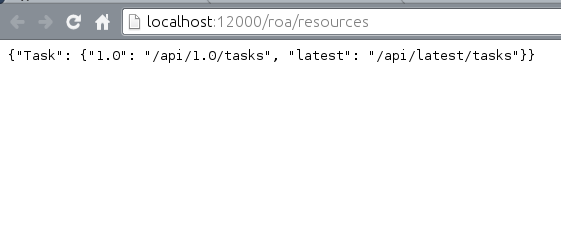
\includegraphics{roa_discovered_resources.png}

\item {} 
Visit \href{http://localhost:12000/api/latest/tasks}{http://localhost:12000/api/latest/tasks}. You should see a response similar to the one below:

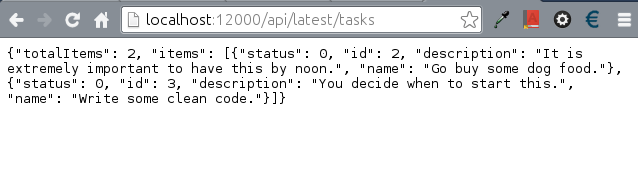
\includegraphics{roa_tasks_initial_listing.png}

\item {} 
Visit \href{http://localhost:12000/api/latest/tasks/1}{http://localhost:12000/api/latest/tasks/1}. You should receive the details for the task with unique identifier 1.

\item {} 
Additionally Create / Update / Delete operations are already working.

\end{enumerate}


\subsubsection{Step 3 - TODO frontend}
\label{how_to/todo/step_3_create_frontend:step-3-todo-frontend}\label{how_to/todo/step_3_create_frontend::doc}
In this section of this tutorial we will develop the frontend for our simple todo application. At this moment you should already
have an API which supports tasks CRUD operations. More over your can order and filter tasks collection and you can request
partial representation of the tasks. (you can find out more on {\hyperref[features/roa::doc]{\emph{ROA (Resource Oriented Architecture)}}} doc page).

For frontend we will quickly develop an application using Backbone.js framework.


\paragraph{Create models}
\label{how_to/todo/step_3_create_frontend:create-models}\begin{enumerate}
\item {} 
git checkout -b step-3-create-frontend

\item {} 
Paste the code below under fantastico-todo/todo/frontend/static/js/bootstrap.js

\begin{Verbatim}[commandchars=\\\{\}]
\PYG{c+cm}{/**}
\PYG{c+cm}{Copyright 2013 Cosnita Radu Viorel}

\PYG{c+cm}{Permission is hereby granted, free of charge, to any person obtaining a copy of this software and associated}
\PYG{c+cm}{documentation files (the \PYGZdq{}Software\PYGZdq{}), to deal in the Software without restriction, including without limitation}
\PYG{c+cm}{the rights to use, copy, modify, merge, publish, distribute, sublicense, and/or sell copies of the Software,}
\PYG{c+cm}{and to permit persons to whom the Software is furnished to do so, subject to the following conditions:}

\PYG{c+cm}{The above copyright notice and this permission notice shall be included in all copies or substantial portions of the Software.}

\PYG{c+cm}{THE SOFTWARE IS PROVIDED \PYGZdq{}AS IS\PYGZdq{}, WITHOUT WARRANTY OF ANY KIND, EXPRESS OR IMPLIED, INCLUDING BUT NOT LIMITED TO THE}
\PYG{c+cm}{WARRANTIES OF MERCHANTABILITY, FITNESS FOR A PARTICULAR PURPOSE AND NONINFRINGEMENT. IN NO EVENT SHALL THE AUTHORS OR}
\PYG{c+cm}{COPYRIGHT HOLDERS BE LIABLE FOR ANY CLAIM, DAMAGES OR OTHER LIABILITY, WHETHER IN AN ACTION OF CONTRACT, TORT OR OTHERWISE,}
\PYG{c+cm}{ARISING FROM, OUT OF OR IN CONNECTION WITH THE SOFTWARE OR THE USE OR OTHER DEALINGS IN THE SOFTWARE.}
\PYG{c+cm}{*/}

\PYG{p}{(}\PYG{k+kd}{function}\PYG{p}{(}\PYG{n+nx}{\PYGZdl{}}\PYG{p}{)} \PYG{p}{\PYGZob{}}
    \PYG{n+nx}{Todo} \PYG{o}{=} \PYG{p}{\PYGZob{}}\PYG{p}{\PYGZcb{}}\PYG{p}{;}

    \PYG{n+nx}{Todo}\PYG{p}{.}\PYG{n+nx}{Models} \PYG{o}{=} \PYG{p}{\PYGZob{}}\PYG{p}{\PYGZcb{}}\PYG{p}{;}
\PYG{p}{\PYGZcb{}}\PYG{p}{)}\PYG{p}{(}\PYG{n+nx}{jQuery}\PYG{p}{)}\PYG{p}{;}
\end{Verbatim}

\item {} 
Paste the code below under fantastico-todo/todo/frontend/static/js/models/resources\_registry.js

\begin{Verbatim}[commandchars=\\\{\}]
\PYG{c+cm}{/**}
\PYG{c+cm}{Copyright 2013 Cosnita Radu Viorel}

\PYG{c+cm}{Permission is hereby granted, free of charge, to any person obtaining a copy of this software and associated}
\PYG{c+cm}{documentation files (the \PYGZdq{}Software\PYGZdq{}), to deal in the Software without restriction, including without limitation}
\PYG{c+cm}{the rights to use, copy, modify, merge, publish, distribute, sublicense, and/or sell copies of the Software,}
\PYG{c+cm}{and to permit persons to whom the Software is furnished to do so, subject to the following conditions:}

\PYG{c+cm}{The above copyright notice and this permission notice shall be included in all copies or substantial portions of the Software.}

\PYG{c+cm}{THE SOFTWARE IS PROVIDED \PYGZdq{}AS IS\PYGZdq{}, WITHOUT WARRANTY OF ANY KIND, EXPRESS OR IMPLIED, INCLUDING BUT NOT LIMITED TO THE}
\PYG{c+cm}{WARRANTIES OF MERCHANTABILITY, FITNESS FOR A PARTICULAR PURPOSE AND NONINFRINGEMENT. IN NO EVENT SHALL THE AUTHORS OR}
\PYG{c+cm}{COPYRIGHT HOLDERS BE LIABLE FOR ANY CLAIM, DAMAGES OR OTHER LIABILITY, WHETHER IN AN ACTION OF CONTRACT, TORT OR OTHERWISE,}
\PYG{c+cm}{ARISING FROM, OUT OF OR IN CONNECTION WITH THE SOFTWARE OR THE USE OR OTHER DEALINGS IN THE SOFTWARE.}
\PYG{c+cm}{*/}

\PYG{p}{(}\PYG{k+kd}{function}\PYG{p}{(}\PYG{n+nx}{\PYGZdl{}}\PYG{p}{)} \PYG{p}{\PYGZob{}}
    \PYG{k+kd}{var} \PYG{n+nx}{registry} \PYG{o}{=} \PYG{p}{\PYGZob{}}\PYG{p}{\PYGZcb{}}\PYG{p}{,}
        \PYG{n+nx}{endpoint} \PYG{o}{=} \PYG{l+s+s2}{\PYGZdq{}/roa/resources\PYGZdq{}}\PYG{p}{;}

    \PYG{c+cm}{/**}
\PYG{c+cm}{     * This model holds the object attributes of a resource. Currently it supports only fetch through collection.}
\PYG{c+cm}{     */}
    \PYG{n+nx}{registry}\PYG{p}{.}\PYG{n+nx}{Resource} \PYG{o}{=} \PYG{n+nx}{Backbone}\PYG{p}{.}\PYG{n+nx}{Model}\PYG{p}{.}\PYG{n+nx}{extend}\PYG{p}{(}\PYG{p}{\PYGZob{}}\PYG{p}{\PYGZcb{}}\PYG{p}{)}\PYG{p}{;}

    \PYG{c+cm}{/**}
\PYG{c+cm}{     * This collection provides access to ROA resources registered to the current project. It is recommended to code each model}
\PYG{c+cm}{     * against the registry so that location changes are not breaking client side code.}
\PYG{c+cm}{     */}
    \PYG{n+nx}{registry}\PYG{p}{.}\PYG{n+nx}{ResourceCollection} \PYG{o}{=} \PYG{n+nx}{Backbone}\PYG{p}{.}\PYG{n+nx}{Collection}\PYG{p}{.}\PYG{n+nx}{extend}\PYG{p}{(}\PYG{p}{\PYGZob{}}
        \PYG{n+nx}{model}\PYG{o}{:} \PYG{n+nx}{registry}\PYG{p}{.}\PYG{n+nx}{Resource}\PYG{p}{,}
        \PYG{n+nx}{url}\PYG{o}{:} \PYG{n+nx}{endpoint}\PYG{p}{,}
        \PYG{c+cm}{/**}
\PYG{c+cm}{         * This method returns the resource url for a given resource name and version. If the version is omitted latest resource}
\PYG{c+cm}{         * url is returned.}
\PYG{c+cm}{         *}
\PYG{c+cm}{         * @param \PYGZob{}String\PYGZcb{} name The name of the resource we want to retrieve discovery information about.}
\PYG{c+cm}{         * @param \PYGZob{}String\PYGZcb{} version (Optional) The version of the resource we want to retrieve discovery information about.}
\PYG{c+cm}{         * @returns The resource url extracted from ROA discovery registry (/roa/resources).}
\PYG{c+cm}{         */}
        \PYG{n+nx}{getResourceUrl}\PYG{o}{:} \PYG{k+kd}{function}\PYG{p}{(}\PYG{n+nx}{name}\PYG{p}{,} \PYG{n+nx}{version}\PYG{p}{)} \PYG{p}{\PYGZob{}}
            \PYG{n+nx}{version} \PYG{o}{=} \PYG{n+nx}{version} \PYG{o}{\textbar{}\textbar{}} \PYG{l+s+s2}{\PYGZdq{}latest\PYGZdq{}}\PYG{p}{;}

            \PYG{k}{if}\PYG{p}{(}\PYG{k}{this}\PYG{p}{.}\PYG{n+nx}{length} \PYG{o}{==} \PYG{l+m+mi}{0}\PYG{p}{)} \PYG{p}{\PYGZob{}}
                \PYG{k}{throw} \PYG{k}{new} \PYG{n+nb}{Error}\PYG{p}{(}\PYG{l+s+s2}{\PYGZdq{}No ROA resources registered.\PYGZdq{}}\PYG{p}{)}\PYG{p}{;}
            \PYG{p}{\PYGZcb{}}

            \PYG{k+kd}{var} \PYG{n+nx}{resources} \PYG{o}{=} \PYG{k}{this}\PYG{p}{.}\PYG{n+nx}{at}\PYG{p}{(}\PYG{l+m+mi}{0}\PYG{p}{)}\PYG{p}{,}
                \PYG{n+nx}{resource} \PYG{o}{=} \PYG{p}{(}\PYG{n+nx}{resources}\PYG{p}{.}\PYG{n+nx}{get}\PYG{p}{(}\PYG{n+nx}{name}\PYG{p}{)} \PYG{o}{\textbar{}\textbar{}} \PYG{p}{\PYGZob{}}\PYG{p}{\PYGZcb{}}\PYG{p}{)}\PYG{p}{[}\PYG{n+nx}{version}\PYG{p}{]}\PYG{p}{;}

            \PYG{k}{if}\PYG{p}{(}\PYG{o}{!}\PYG{n+nx}{resource}\PYG{p}{)} \PYG{p}{\PYGZob{}}
                \PYG{k}{throw} \PYG{k}{new} \PYG{n+nb}{Error}\PYG{p}{(}\PYG{l+s+s2}{\PYGZdq{}Resource \PYGZdq{}} \PYG{o}{+} \PYG{n+nx}{name} \PYG{o}{+} \PYG{l+s+s2}{\PYGZdq{}, version \PYGZdq{}} \PYG{o}{+} \PYG{n+nx}{version} \PYG{o}{+} \PYG{l+s+s2}{\PYGZdq{} is not registered.\PYGZdq{}}\PYG{p}{)}\PYG{p}{;}
            \PYG{p}{\PYGZcb{}}

            \PYG{k}{return} \PYG{n+nx}{resource}\PYG{p}{;}
        \PYG{p}{\PYGZcb{}}
    \PYG{p}{\PYGZcb{}}\PYG{p}{)}\PYG{p}{;}

    \PYG{n+nx}{Todo}\PYG{p}{.}\PYG{n+nx}{Models}\PYG{p}{.}\PYG{n+nx}{Registry} \PYG{o}{=} \PYG{k}{new} \PYG{n+nx}{registry}\PYG{p}{.}\PYG{n+nx}{ResourceCollection}\PYG{p}{(}\PYG{p}{)}\PYG{p}{;}
    \PYG{n+nx}{Todo}\PYG{p}{.}\PYG{n+nx}{Models}\PYG{p}{.}\PYG{n+nx}{Registry}\PYG{p}{.}\PYG{n+nx}{loader} \PYG{o}{=} \PYG{n+nx}{Todo}\PYG{p}{.}\PYG{n+nx}{Models}\PYG{p}{.}\PYG{n+nx}{Registry}\PYG{p}{.}\PYG{n+nx}{fetch}\PYG{p}{(}\PYG{p}{)}\PYG{p}{;}
\PYG{p}{\PYGZcb{}}\PYG{p}{)}\PYG{p}{(}\PYG{n+nx}{jQuery}\PYG{p}{)}\PYG{p}{;}
\end{Verbatim}

\item {} 
Paste the code below under fantastico-todo/todo/frontend/static/js/models/tasks.js

\begin{Verbatim}[commandchars=\\\{\}]
\PYG{c+cm}{/**}
\PYG{c+cm}{Copyright 2013 Cosnita Radu Viorel}

\PYG{c+cm}{Permission is hereby granted, free of charge, to any person obtaining a copy of this software and associated}
\PYG{c+cm}{documentation files (the \PYGZdq{}Software\PYGZdq{}), to deal in the Software without restriction, including without limitation}
\PYG{c+cm}{the rights to use, copy, modify, merge, publish, distribute, sublicense, and/or sell copies of the Software,}
\PYG{c+cm}{and to permit persons to whom the Software is furnished to do so, subject to the following conditions:}

\PYG{c+cm}{The above copyright notice and this permission notice shall be included in all copies or substantial portions of the Software.}

\PYG{c+cm}{THE SOFTWARE IS PROVIDED \PYGZdq{}AS IS\PYGZdq{}, WITHOUT WARRANTY OF ANY KIND, EXPRESS OR IMPLIED, INCLUDING BUT NOT LIMITED TO THE}
\PYG{c+cm}{WARRANTIES OF MERCHANTABILITY, FITNESS FOR A PARTICULAR PURPOSE AND NONINFRINGEMENT. IN NO EVENT SHALL THE AUTHORS OR}
\PYG{c+cm}{COPYRIGHT HOLDERS BE LIABLE FOR ANY CLAIM, DAMAGES OR OTHER LIABILITY, WHETHER IN AN ACTION OF CONTRACT, TORT OR OTHERWISE,}
\PYG{c+cm}{ARISING FROM, OUT OF OR IN CONNECTION WITH THE SOFTWARE OR THE USE OR OTHER DEALINGS IN THE SOFTWARE.}
\PYG{c+cm}{*/}

\PYG{p}{(}\PYG{k+kd}{function}\PYG{p}{(}\PYG{n+nx}{\PYGZdl{}}\PYG{p}{)} \PYG{p}{\PYGZob{}}
    \PYG{k+kd}{var} \PYG{n+nx}{tasks} \PYG{o}{=} \PYG{p}{\PYGZob{}}\PYG{p}{\PYGZcb{}}\PYG{p}{;}

    \PYG{k+kd}{function} \PYG{n+nx}{getTasksUrl}\PYG{p}{(}\PYG{p}{)} \PYG{p}{\PYGZob{}}
        \PYG{k}{return} \PYG{n+nx}{Todo}\PYG{p}{.}\PYG{n+nx}{Models}\PYG{p}{.}\PYG{n+nx}{Registry}\PYG{p}{.}\PYG{n+nx}{getResourceUrl}\PYG{p}{(}\PYG{l+s+s2}{\PYGZdq{}Task\PYGZdq{}}\PYG{p}{)}\PYG{p}{;}
    \PYG{p}{\PYGZcb{}}

    \PYG{n+nx}{tasks}\PYG{p}{.}\PYG{n+nx}{Task} \PYG{o}{=} \PYG{n+nx}{Backbone}\PYG{p}{.}\PYG{n+nx}{Model}\PYG{p}{.}\PYG{n+nx}{extend}\PYG{p}{(}\PYG{p}{\PYGZob{}}
        \PYG{n+nx}{idAttribute}\PYG{o}{:} \PYG{l+s+s2}{\PYGZdq{}task\PYGZus{}id\PYGZdq{}}\PYG{p}{,}
        \PYG{n+nx}{urlRoot}\PYG{o}{:} \PYG{n+nx}{getTasksUrl}
    \PYG{p}{\PYGZcb{}}\PYG{p}{)}\PYG{p}{;}

    \PYG{n+nx}{tasks}\PYG{p}{.}\PYG{n+nx}{TaskCollection} \PYG{o}{=} \PYG{n+nx}{Backbone}\PYG{p}{.}\PYG{n+nx}{Collection}\PYG{p}{.}\PYG{n+nx}{extend}\PYG{p}{(}\PYG{p}{\PYGZob{}}
        \PYG{n+nx}{model}\PYG{o}{:} \PYG{n+nx}{tasks}\PYG{p}{.}\PYG{n+nx}{Task}\PYG{p}{,}
        \PYG{c+cm}{/**}
\PYG{c+cm}{         * This method is overriden so that it guarantees tasks are ordered alphabetically and only id and name attributes are}
\PYG{c+cm}{         * returned for each available task (partial resource representation).}
\PYG{c+cm}{         */}
        \PYG{n+nx}{url}\PYG{o}{:} \PYG{k+kd}{function}\PYG{p}{(}\PYG{p}{)} \PYG{p}{\PYGZob{}}
            \PYG{k+kd}{var} \PYG{n+nx}{url} \PYG{o}{=} \PYG{p}{[}\PYG{n+nx}{getTasksUrl}\PYG{p}{(}\PYG{p}{)}\PYG{p}{]}\PYG{p}{;}
            \PYG{n+nx}{url}\PYG{p}{.}\PYG{n+nx}{push}\PYG{p}{(}\PYG{l+s+s2}{\PYGZdq{}?\PYGZdq{}}\PYG{p}{)}\PYG{p}{;}

            \PYG{k}{if}\PYG{p}{(}\PYG{k}{this}\PYG{p}{.}\PYG{n+nx}{\PYGZus{}offset}\PYG{p}{)} \PYG{p}{\PYGZob{}}
                \PYG{n+nx}{url}\PYG{p}{.}\PYG{n+nx}{push}\PYG{p}{(}\PYG{l+s+s2}{\PYGZdq{}offset=\PYGZdq{}} \PYG{o}{+} \PYG{k}{this}\PYG{p}{.}\PYG{n+nx}{\PYGZus{}offset}\PYG{p}{)}\PYG{p}{;}
            \PYG{p}{\PYGZcb{}}

            \PYG{k}{if}\PYG{p}{(}\PYG{k}{this}\PYG{p}{.}\PYG{n+nx}{\PYGZus{}limit}\PYG{p}{)} \PYG{p}{\PYGZob{}}
                \PYG{n+nx}{url}\PYG{p}{.}\PYG{n+nx}{push}\PYG{p}{(}\PYG{l+s+s2}{\PYGZdq{}\PYGZam{}limit=\PYGZdq{}} \PYG{o}{+} \PYG{k}{this}\PYG{p}{.}\PYG{n+nx}{\PYGZus{}limit}\PYG{p}{)}\PYG{p}{;}
            \PYG{p}{\PYGZcb{}}

            \PYG{n+nx}{url}\PYG{p}{.}\PYG{n+nx}{push}\PYG{p}{(}\PYG{l+s+s2}{\PYGZdq{}\PYGZam{}fields=task\PYGZus{}id,name,status\PYGZdq{}}\PYG{p}{)}\PYG{p}{;}
            \PYG{n+nx}{url}\PYG{p}{.}\PYG{n+nx}{push}\PYG{p}{(}\PYG{l+s+s2}{\PYGZdq{}\PYGZam{}order=asc(name)\PYGZdq{}}\PYG{p}{)}\PYG{p}{;}

            \PYG{k}{return} \PYG{n+nx}{url}\PYG{p}{.}\PYG{n+nx}{join}\PYG{p}{(}\PYG{l+s+s2}{\PYGZdq{}\PYGZdq{}}\PYG{p}{)}\PYG{p}{;}
        \PYG{p}{\PYGZcb{}}\PYG{p}{,}
        \PYG{c+cm}{/**}
\PYG{c+cm}{         * In comparison with standard backbone collection fetch, ROA collections support pagination. This is why options is}
\PYG{c+cm}{         * parsed before actually fetching the collection.}
\PYG{c+cm}{         */}
        \PYG{n+nx}{fetch}\PYG{o}{:} \PYG{k+kd}{function}\PYG{p}{(}\PYG{n+nx}{options}\PYG{p}{)} \PYG{p}{\PYGZob{}}
            \PYG{n+nx}{options} \PYG{o}{=} \PYG{n+nx}{options} \PYG{o}{\textbar{}\textbar{}} \PYG{p}{\PYGZob{}}\PYG{p}{\PYGZcb{}}\PYG{p}{;}

            \PYG{k}{this}\PYG{p}{.}\PYG{n+nx}{\PYGZus{}offset} \PYG{o}{=} \PYG{n+nx}{options}\PYG{p}{.}\PYG{n+nx}{offset}\PYG{p}{;}
            \PYG{k}{this}\PYG{p}{.}\PYG{n+nx}{\PYGZus{}limit} \PYG{o}{=} \PYG{n+nx}{options}\PYG{p}{.}\PYG{n+nx}{limit}\PYG{p}{;}

            \PYG{k}{return} \PYG{n+nx}{Backbone}\PYG{p}{.}\PYG{n+nx}{Collection}\PYG{p}{.}\PYG{n+nx}{prototype}\PYG{p}{.}\PYG{n+nx}{fetch}\PYG{p}{.}\PYG{n+nx}{call}\PYG{p}{(}\PYG{k}{this}\PYG{p}{,} \PYG{n+nx}{options}\PYG{p}{)}\PYG{p}{;}
        \PYG{p}{\PYGZcb{}}\PYG{p}{,}
        \PYG{c+cm}{/**}
\PYG{c+cm}{         * This method save the items returned form REST ROA api to this backbone collection. Additionally it adds the total}
\PYG{c+cm}{         * items counter as collection property.}
\PYG{c+cm}{         *}
\PYG{c+cm}{         * @param \PYGZob{}Object\PYGZcb{} response The http response coming for /api/latest/tasks collection.}
\PYG{c+cm}{         */}
        \PYG{n+nx}{parse}\PYG{o}{:} \PYG{k+kd}{function}\PYG{p}{(}\PYG{n+nx}{response}\PYG{p}{)} \PYG{p}{\PYGZob{}}
            \PYG{k}{this}\PYG{p}{.}\PYG{n+nx}{totalItems} \PYG{o}{=} \PYG{n+nx}{response}\PYG{p}{.}\PYG{n+nx}{totalItems}\PYG{p}{;}

            \PYG{k}{return} \PYG{n+nx}{response}\PYG{p}{.}\PYG{n+nx}{items}\PYG{p}{;}
        \PYG{p}{\PYGZcb{}}
    \PYG{p}{\PYGZcb{}}\PYG{p}{)}\PYG{p}{;}

    \PYG{n+nx}{Todo}\PYG{p}{.}\PYG{n+nx}{Models}\PYG{p}{.}\PYG{n+nx}{Tasks} \PYG{o}{=} \PYG{n+nx}{tasks}\PYG{p}{;}
\PYG{p}{\PYGZcb{}}\PYG{p}{)}\PYG{p}{(}\PYG{n+nx}{jQuery}\PYG{p}{)}\PYG{p}{;}
\end{Verbatim}

\end{enumerate}

We have all models in place so we are going to implement the frontend of the application in the next section.


\subparagraph{Models implementation notes}
\label{how_to/todo/step_3_create_frontend:models-implementation-notes}
In Fantastico, there is a resource registry which can be used for discovery. It is recommended to always use it to obtain your
models api urls. This will guarantee that any change of API location on server side is automatically propagated on client side.

In addition because our application is not going to use description we optimized the client side code by using ROA partial resource
representation. More over, the resources are ordered alphabetically by name.

ROA collections support pagination out of the box and tasks client side implementation shows how easily it is to provide it
for client side code.

For better understanding all the concepts used in this section you can read {\hyperref[features/roa::doc]{\emph{ROA (Resource Oriented Architecture)}}}.

In addition you probably noticed that static assets are created under a special folder named \textbf{static}. This allows us to easily
serve static assets from a cache server or cdn in production. You can read more about this on {\hyperref[how_to/static_assets::doc]{\emph{Static assets}}}.


\paragraph{Create frontend}
\label{how_to/todo/step_3_create_frontend:create-frontend}
In this section we are going to create all routes used in frontend:
\begin{enumerate}
\item {} 
/frontend/ui/index

\item {} 
/frontend/ui/tasks-list-menu

\item {} 
/frontend/ui/tasks-list-content

\item {} 
/frontend/ui/tasks-list-pager

\end{enumerate}

This approach allows us to have a very clear separation and control of listing components of TODO application. In order to create
the frontend follow the steps below:
\begin{enumerate}
\item {} 
Paste the following code under fantastico-todo/todo/frontend/todo\_ui.py:

\begin{Verbatim}[commandchars=\\\{\}]
\PYG{l+s+sd}{\PYGZsq{}\PYGZsq{}\PYGZsq{}}
\PYG{l+s+sd}{Copyright 2013 Cosnita Radu Viorel}

\PYG{l+s+sd}{Permission is hereby granted, free of charge, to any person obtaining a copy of this software and associated}
\PYG{l+s+sd}{documentation files (the \PYGZdq{}Software\PYGZdq{}), to deal in the Software without restriction, including without limitation}
\PYG{l+s+sd}{the rights to use, copy, modify, merge, publish, distribute, sublicense, and/or sell copies of the Software,}
\PYG{l+s+sd}{and to permit persons to whom the Software is furnished to do so, subject to the following conditions:}

\PYG{l+s+sd}{The above copyright notice and this permission notice shall be included in all copies or substantial portions of the Software.}

\PYG{l+s+sd}{THE SOFTWARE IS PROVIDED \PYGZdq{}AS IS\PYGZdq{}, WITHOUT WARRANTY OF ANY KIND, EXPRESS OR IMPLIED, INCLUDING BUT NOT LIMITED TO THE}
\PYG{l+s+sd}{WARRANTIES OF MERCHANTABILITY, FITNESS FOR A PARTICULAR PURPOSE AND NONINFRINGEMENT. IN NO EVENT SHALL THE AUTHORS OR}
\PYG{l+s+sd}{COPYRIGHT HOLDERS BE LIABLE FOR ANY CLAIM, DAMAGES OR OTHER LIABILITY, WHETHER IN AN ACTION OF CONTRACT, TORT OR OTHERWISE,}
\PYG{l+s+sd}{ARISING FROM, OUT OF OR IN CONNECTION WITH THE SOFTWARE OR THE USE OR OTHER DEALINGS IN THE SOFTWARE.}

\PYG{l+s+sd}{.. codeauthor:: Radu Viorel Cosnita \PYGZlt{}radu.cosnita@gmail.com\PYGZgt{}}
\PYG{l+s+sd}{.. py:module:: todo.frontend.ui}
\PYG{l+s+sd}{\PYGZsq{}\PYGZsq{}\PYGZsq{}}

\PYG{k+kn}{from} \PYG{n+nn}{fantastico.mvc.base\PYGZus{}controller} \PYG{k+kn}{import} \PYG{n}{BaseController}
\PYG{k+kn}{from} \PYG{n+nn}{fantastico.mvc.controller\PYGZus{}decorators} \PYG{k+kn}{import} \PYG{n}{Controller}\PYG{p}{,} \PYG{n}{ControllerProvider}
\PYG{k+kn}{from} \PYG{n+nn}{webob.response} \PYG{k+kn}{import} \PYG{n}{Response}

\PYG{n+nd}{@ControllerProvider}\PYG{p}{(}\PYG{p}{)}
\PYG{k}{class} \PYG{n+nc}{TodoUi}\PYG{p}{(}\PYG{n}{BaseController}\PYG{p}{)}\PYG{p}{:}
    \PYG{l+s+sd}{\PYGZsq{}\PYGZsq{}\PYGZsq{}This class provides all routes used by todo frontend application.\PYGZsq{}\PYGZsq{}\PYGZsq{}}

    \PYG{n+nd}{@Controller}\PYG{p}{(}\PYG{n}{url}\PYG{o}{=}\PYG{l+s}{\PYGZdq{}}\PYG{l+s}{/frontend/ui/index}\PYG{l+s}{\PYGZdq{}}\PYG{p}{)}
    \PYG{k}{def} \PYG{n+nf}{get\PYGZus{}index}\PYG{p}{(}\PYG{n+nb+bp}{self}\PYG{p}{,} \PYG{n}{request}\PYG{p}{)}\PYG{p}{:}
        \PYG{l+s+sd}{\PYGZsq{}\PYGZsq{}\PYGZsq{}This method returns the index of todo ui application.\PYGZsq{}\PYGZsq{}\PYGZsq{}}

        \PYG{n}{content} \PYG{o}{=} \PYG{n+nb+bp}{self}\PYG{o}{.}\PYG{n}{load\PYGZus{}template}\PYG{p}{(}\PYG{l+s}{\PYGZdq{}}\PYG{l+s}{listing.html}\PYG{l+s}{\PYGZdq{}}\PYG{p}{)}

        \PYG{k}{return} \PYG{n}{Response}\PYG{p}{(}\PYG{n}{content}\PYG{p}{)}

    \PYG{n+nd}{@Controller}\PYG{p}{(}\PYG{n}{url}\PYG{o}{=}\PYG{l+s}{\PYGZdq{}}\PYG{l+s}{/frontend/ui/tasks\PYGZhy{}list\PYGZhy{}menu}\PYG{l+s}{\PYGZdq{}}\PYG{p}{)}
    \PYG{k}{def} \PYG{n+nf}{get\PYGZus{}tasks\PYGZus{}menu}\PYG{p}{(}\PYG{n+nb+bp}{self}\PYG{p}{,} \PYG{n}{request}\PYG{p}{)}\PYG{p}{:}
        \PYG{l+s+sd}{\PYGZsq{}\PYGZsq{}\PYGZsq{}This method return the tasks list menu.\PYGZsq{}\PYGZsq{}\PYGZsq{}}

        \PYG{n}{content} \PYG{o}{=} \PYG{n+nb+bp}{self}\PYG{o}{.}\PYG{n}{load\PYGZus{}template}\PYG{p}{(}\PYG{l+s}{\PYGZdq{}}\PYG{l+s}{listing\PYGZus{}menu.html}\PYG{l+s}{\PYGZdq{}}\PYG{p}{)}

        \PYG{k}{return} \PYG{n}{Response}\PYG{p}{(}\PYG{n}{content}\PYG{p}{)}

    \PYG{n+nd}{@Controller}\PYG{p}{(}\PYG{n}{url}\PYG{o}{=}\PYG{l+s}{\PYGZdq{}}\PYG{l+s}{/frontend/ui/tasks\PYGZhy{}list\PYGZhy{}content}\PYG{l+s}{\PYGZdq{}}\PYG{p}{)}
    \PYG{k}{def} \PYG{n+nf}{get\PYGZus{}tasks\PYGZus{}content}\PYG{p}{(}\PYG{n+nb+bp}{self}\PYG{p}{,} \PYG{n}{request}\PYG{p}{)}\PYG{p}{:}
        \PYG{l+s+sd}{\PYGZsq{}\PYGZsq{}\PYGZsq{}This method returns the markup for tasks listing content area.\PYGZsq{}\PYGZsq{}\PYGZsq{}}

        \PYG{n}{content} \PYG{o}{=} \PYG{n+nb+bp}{self}\PYG{o}{.}\PYG{n}{load\PYGZus{}template}\PYG{p}{(}\PYG{l+s}{\PYGZdq{}}\PYG{l+s}{listing\PYGZus{}content.html}\PYG{l+s}{\PYGZdq{}}\PYG{p}{)}

        \PYG{k}{return} \PYG{n}{Response}\PYG{p}{(}\PYG{n}{content}\PYG{p}{)}

    \PYG{n+nd}{@Controller}\PYG{p}{(}\PYG{n}{url}\PYG{o}{=}\PYG{l+s}{\PYGZdq{}}\PYG{l+s}{/frontend/ui/tasks\PYGZhy{}list\PYGZhy{}pager}\PYG{l+s}{\PYGZdq{}}\PYG{p}{)}
    \PYG{k}{def} \PYG{n+nf}{get\PYGZus{}tasks\PYGZus{}pager}\PYG{p}{(}\PYG{n+nb+bp}{self}\PYG{p}{,} \PYG{n}{request}\PYG{p}{)}\PYG{p}{:}
        \PYG{l+s+sd}{\PYGZsq{}\PYGZsq{}\PYGZsq{}This method returns the markup for tasks listing pagination area.\PYGZsq{}\PYGZsq{}\PYGZsq{}}

        \PYG{n}{content} \PYG{o}{=} \PYG{n+nb+bp}{self}\PYG{o}{.}\PYG{n}{load\PYGZus{}template}\PYG{p}{(}\PYG{l+s}{\PYGZdq{}}\PYG{l+s}{listing\PYGZus{}pager.html}\PYG{l+s}{\PYGZdq{}}\PYG{p}{)}

        \PYG{k}{return} \PYG{n}{Response}\PYG{p}{(}\PYG{n}{content}\PYG{p}{)}
\end{Verbatim}

\end{enumerate}

The final step of this tutorial requires the creation of controller code for listing tasks and CRUD operations:
\begin{enumerate}
\item {} 
Paste the code below under fantastico-todo/todo/frontend/static/js/list\_tasks.js:

\begin{Verbatim}[commandchars=\\\{\}]
\PYG{c+cm}{/**}
\PYG{c+cm}{Copyright 2013 Cosnita Radu Viorel}

\PYG{c+cm}{Permission is hereby granted, free of charge, to any person obtaining a copy of this software and associated}
\PYG{c+cm}{documentation files (the \PYGZdq{}Software\PYGZdq{}), to deal in the Software without restriction, including without limitation}
\PYG{c+cm}{the rights to use, copy, modify, merge, publish, distribute, sublicense, and/or sell copies of the Software,}
\PYG{c+cm}{and to permit persons to whom the Software is furnished to do so, subject to the following conditions:}

\PYG{c+cm}{The above copyright notice and this permission notice shall be included in all copies or substantial portions of the Software.}

\PYG{c+cm}{THE SOFTWARE IS PROVIDED \PYGZdq{}AS IS\PYGZdq{}, WITHOUT WARRANTY OF ANY KIND, EXPRESS OR IMPLIED, INCLUDING BUT NOT LIMITED TO THE}
\PYG{c+cm}{WARRANTIES OF MERCHANTABILITY, FITNESS FOR A PARTICULAR PURPOSE AND NONINFRINGEMENT. IN NO EVENT SHALL THE AUTHORS OR}
\PYG{c+cm}{COPYRIGHT HOLDERS BE LIABLE FOR ANY CLAIM, DAMAGES OR OTHER LIABILITY, WHETHER IN AN ACTION OF CONTRACT, TORT OR OTHERWISE,}
\PYG{c+cm}{ARISING FROM, OUT OF OR IN CONNECTION WITH THE SOFTWARE OR THE USE OR OTHER DEALINGS IN THE SOFTWARE.}
\PYG{c+cm}{*/}

\PYG{p}{(}\PYG{k+kd}{function}\PYG{p}{(}\PYG{n+nx}{\PYGZdl{}}\PYG{p}{)} \PYG{p}{\PYGZob{}}
    \PYG{n+nx}{TPL\PYGZus{}TASK} \PYG{o}{=} \PYG{p}{[}\PYG{l+s+s1}{\PYGZsq{}\PYGZlt{}div class=\PYGZdq{}task\PYGZdq{}\PYGZgt{}\PYGZsq{}}\PYG{p}{]}\PYG{p}{;}
    \PYG{n+nx}{TPL\PYGZus{}TASK}\PYG{p}{.}\PYG{n+nx}{push}\PYG{p}{(}\PYG{l+s+s1}{\PYGZsq{}\PYGZlt{}div class=\PYGZdq{}input\PYGZhy{}group\PYGZdq{}\PYGZgt{}\PYGZsq{}}\PYG{p}{)}\PYG{p}{;}
    \PYG{n+nx}{TPL\PYGZus{}TASK}\PYG{p}{.}\PYG{n+nx}{push}\PYG{p}{(}\PYG{l+s+s1}{\PYGZsq{}\PYGZlt{}span class=\PYGZdq{}input\PYGZhy{}group\PYGZhy{}addon\PYGZdq{}\PYGZgt{}\PYGZsq{}}\PYG{p}{)}\PYG{p}{;}
    \PYG{n+nx}{TPL\PYGZus{}TASK}\PYG{p}{.}\PYG{n+nx}{push}\PYG{p}{(}\PYG{l+s+s1}{\PYGZsq{}\PYGZlt{}input type=\PYGZdq{}checkbox\PYGZdq{} data\PYGZhy{}role=\PYGZdq{}tasks\PYGZhy{}complete\PYGZdq{} data\PYGZhy{}tid=\PYGZdq{}\PYGZlt{}\PYGZpc{}= task.get(\PYGZbs{}\PYGZdq{}task\PYGZus{}id\PYGZbs{}\PYGZdq{}) \PYGZpc{}\PYGZgt{}\PYGZdq{} /\PYGZgt{}\PYGZsq{}}\PYG{p}{)}\PYG{p}{;}
    \PYG{n+nx}{TPL\PYGZus{}TASK}\PYG{p}{.}\PYG{n+nx}{push}\PYG{p}{(}\PYG{l+s+s1}{\PYGZsq{}\PYGZlt{}/span\PYGZgt{}\PYGZsq{}}\PYG{p}{)}\PYG{p}{;}
    \PYG{n+nx}{TPL\PYGZus{}TASK}\PYG{p}{.}\PYG{n+nx}{push}\PYG{p}{(}\PYG{l+s+s1}{\PYGZsq{}\PYGZlt{}\PYGZpc{} if(task.get(\PYGZdq{}status\PYGZdq{}) === 0) \PYGZob{} \PYGZpc{}\PYGZgt{}\PYGZsq{}}\PYG{p}{)}\PYG{p}{;}
    \PYG{n+nx}{TPL\PYGZus{}TASK}\PYG{p}{.}\PYG{n+nx}{push}\PYG{p}{(}\PYG{l+s+s1}{\PYGZsq{}\PYGZlt{}h3 class=\PYGZdq{}form\PYGZhy{}control\PYGZdq{}\PYGZgt{}\PYGZlt{}\PYGZpc{}= task.get(\PYGZbs{}\PYGZdq{}name\PYGZbs{}\PYGZdq{}) \PYGZpc{}\PYGZgt{}\PYGZlt{}/h3\PYGZgt{}\PYGZsq{}}\PYG{p}{)}\PYG{p}{;}
    \PYG{n+nx}{TPL\PYGZus{}TASK}\PYG{p}{.}\PYG{n+nx}{push}\PYG{p}{(}\PYG{l+s+s1}{\PYGZsq{}\PYGZlt{}\PYGZpc{} \PYGZcb{} else \PYGZob{} \PYGZpc{}\PYGZgt{}\PYGZsq{}}\PYG{p}{)}\PYG{p}{;}
    \PYG{n+nx}{TPL\PYGZus{}TASK}\PYG{p}{.}\PYG{n+nx}{push}\PYG{p}{(}\PYG{l+s+s1}{\PYGZsq{}\PYGZlt{}h3 class=\PYGZdq{}form\PYGZhy{}control task\PYGZhy{}completed\PYGZdq{}\PYGZgt{}\PYGZlt{}\PYGZpc{}= task.get(\PYGZbs{}\PYGZdq{}name\PYGZbs{}\PYGZdq{}) \PYGZpc{}\PYGZgt{}\PYGZlt{}/h3\PYGZgt{}\PYGZsq{}}\PYG{p}{)}\PYG{p}{;}
    \PYG{n+nx}{TPL\PYGZus{}TASK}\PYG{p}{.}\PYG{n+nx}{push}\PYG{p}{(}\PYG{l+s+s1}{\PYGZsq{}\PYGZlt{}\PYGZpc{} \PYGZcb{} \PYGZpc{}\PYGZgt{}\PYGZsq{}}\PYG{p}{)}\PYG{p}{;}
    \PYG{n+nx}{TPL\PYGZus{}TASK}\PYG{p}{.}\PYG{n+nx}{push}\PYG{p}{(}\PYG{l+s+s2}{\PYGZdq{}\PYGZlt{}/div\PYGZgt{}\PYGZdq{}}\PYG{p}{)}\PYG{p}{;}
    \PYG{n+nx}{TPL\PYGZus{}TASK}\PYG{p}{.}\PYG{n+nx}{push}\PYG{p}{(}\PYG{l+s+s2}{\PYGZdq{}\PYGZlt{}hr/\PYGZgt{}\PYGZdq{}}\PYG{p}{)}\PYG{p}{;}
    \PYG{n+nx}{TPL\PYGZus{}TASK}\PYG{p}{.}\PYG{n+nx}{push}\PYG{p}{(}\PYG{l+s+s2}{\PYGZdq{}\PYGZlt{}/div\PYGZgt{}\PYGZdq{}}\PYG{p}{)}\PYG{p}{;}

    \PYG{n+nx}{TPL\PYGZus{}TASK} \PYG{o}{=} \PYG{n+nx}{TPL\PYGZus{}TASK}\PYG{p}{.}\PYG{n+nx}{join}\PYG{p}{(}\PYG{l+s+s2}{\PYGZdq{}\PYGZdq{}}\PYG{p}{)}\PYG{p}{;}

    \PYG{k+kd}{function} \PYG{n+nx}{ListingController}\PYG{p}{(}\PYG{p}{)} \PYG{p}{\PYGZob{}}
        \PYG{k}{this}\PYG{p}{.}\PYG{n+nx}{\PYGZus{}tasks} \PYG{o}{=} \PYG{k}{new} \PYG{n+nx}{Todo}\PYG{p}{.}\PYG{n+nx}{Models}\PYG{p}{.}\PYG{n+nx}{Tasks}\PYG{p}{.}\PYG{n+nx}{TaskCollection}\PYG{p}{(}\PYG{p}{)}\PYG{p}{;}
        \PYG{k}{this}\PYG{p}{.}\PYG{n+nx}{\PYGZus{}offset} \PYG{o}{=} \PYG{l+m+mi}{0}\PYG{p}{;}
        \PYG{k}{this}\PYG{p}{.}\PYG{n+nx}{\PYGZus{}limit} \PYG{o}{=} \PYG{l+m+mi}{10}\PYG{p}{;}
        \PYG{k}{this}\PYG{p}{.}\PYG{n+nx}{\PYGZus{}fetchMoreSize} \PYG{o}{=} \PYG{l+m+mi}{5}\PYG{p}{;}
    \PYG{p}{\PYGZcb{}}\PYG{p}{;}

    \PYG{n+nx}{ListingController}\PYG{p}{.}\PYG{n+nx}{prototype}\PYG{p}{.}\PYG{n+nx}{start} \PYG{o}{=} \PYG{k+kd}{function}\PYG{p}{(}\PYG{p}{)} \PYG{p}{\PYGZob{}}
        \PYG{k}{this}\PYG{p}{.}\PYG{n+nx}{\PYGZus{}tfNewTask} \PYG{o}{=} \PYG{n+nx}{\PYGZdl{}}\PYG{p}{(}\PYG{l+s+s2}{\PYGZdq{}\PYGZsh{}txt\PYGZhy{}new\PYGZhy{}task\PYGZdq{}}\PYG{p}{)}\PYG{p}{;}
        \PYG{k}{this}\PYG{p}{.}\PYG{n+nx}{\PYGZus{}btnComplete} \PYG{o}{=} \PYG{n+nx}{\PYGZdl{}}\PYG{p}{(}\PYG{l+s+s2}{\PYGZdq{}\PYGZsh{}btn\PYGZhy{}complete\PYGZhy{}task\PYGZdq{}}\PYG{p}{)}\PYG{p}{;}
        \PYG{k}{this}\PYG{p}{.}\PYG{n+nx}{\PYGZus{}btnRemove} \PYG{o}{=} \PYG{n+nx}{\PYGZdl{}}\PYG{p}{(}\PYG{l+s+s2}{\PYGZdq{}\PYGZsh{}btn\PYGZhy{}remove\PYGZhy{}task\PYGZdq{}}\PYG{p}{)}\PYG{p}{;}
        \PYG{k}{this}\PYG{p}{.}\PYG{n+nx}{\PYGZus{}tasksArea} \PYG{o}{=} \PYG{n+nx}{\PYGZdl{}}\PYG{p}{(}\PYG{l+s+s2}{\PYGZdq{}.tasks\PYGZhy{}area\PYGZdq{}}\PYG{p}{)}\PYG{p}{;}
        \PYG{k}{this}\PYG{p}{.}\PYG{n+nx}{\PYGZus{}pagerText} \PYG{o}{=} \PYG{n+nx}{\PYGZdl{}}\PYG{p}{(}\PYG{l+s+s2}{\PYGZdq{}.tasks\PYGZhy{}pager\PYGZdq{}}\PYG{p}{)}\PYG{p}{.}\PYG{n+nx}{find}\PYG{p}{(}\PYG{l+s+s2}{\PYGZdq{}p\PYGZdq{}}\PYG{p}{)}\PYG{p}{;}
        \PYG{k}{this}\PYG{p}{.}\PYG{n+nx}{\PYGZus{}btnPagerFetch} \PYG{o}{=} \PYG{n+nx}{\PYGZdl{}}\PYG{p}{(}\PYG{l+s+s2}{\PYGZdq{}.tasks\PYGZhy{}pager\PYGZdq{}}\PYG{p}{)}\PYG{p}{.}\PYG{n+nx}{find}\PYG{p}{(}\PYG{l+s+s2}{\PYGZdq{}button\PYGZdq{}}\PYG{p}{)}\PYG{p}{;}

        \PYG{k}{this}\PYG{p}{.}\PYG{n+nx}{\PYGZus{}initEvents}\PYG{p}{(}\PYG{p}{)}\PYG{p}{;}
    \PYG{p}{\PYGZcb{}}\PYG{p}{;}

    \PYG{n+nx}{ListingController}\PYG{p}{.}\PYG{n+nx}{prototype}\PYG{p}{.}\PYG{n+nx}{\PYGZus{}getSelectedTasks} \PYG{o}{=} \PYG{k+kd}{function}\PYG{p}{(}\PYG{p}{)} \PYG{p}{\PYGZob{}}
        \PYG{k+kd}{var} \PYG{n+nx}{ids} \PYG{o}{=} \PYG{p}{[}\PYG{p}{]}\PYG{p}{,}
            \PYG{n+nx}{tasksChk} \PYG{o}{=} \PYG{k}{this}\PYG{p}{.}\PYG{n+nx}{\PYGZus{}tasksArea}\PYG{p}{.}\PYG{n+nx}{find}\PYG{p}{(}\PYG{l+s+s2}{\PYGZdq{}input[data\PYGZhy{}role=\PYGZsq{}tasks\PYGZhy{}complete\PYGZsq{}]\PYGZdq{}}\PYG{p}{)}\PYG{p}{;}

        \PYG{n+nx}{\PYGZus{}}\PYG{p}{.}\PYG{n+nx}{each}\PYG{p}{(}\PYG{n+nx}{tasksChk}\PYG{p}{,} \PYG{k+kd}{function}\PYG{p}{(}\PYG{n+nx}{item}\PYG{p}{)} \PYG{p}{\PYGZob{}}
            \PYG{n+nx}{item} \PYG{o}{=} \PYG{n+nx}{\PYGZdl{}}\PYG{p}{(}\PYG{n+nx}{item}\PYG{p}{)}\PYG{p}{;}

            \PYG{k}{if}\PYG{p}{(}\PYG{o}{!}\PYG{n+nx}{item}\PYG{p}{.}\PYG{n+nx}{is}\PYG{p}{(}\PYG{l+s+s2}{\PYGZdq{}:checked\PYGZdq{}}\PYG{p}{)}\PYG{p}{)} \PYG{p}{\PYGZob{}}
                \PYG{k}{return}\PYG{p}{;}
            \PYG{p}{\PYGZcb{}}

            \PYG{n+nx}{ids}\PYG{p}{.}\PYG{n+nx}{push}\PYG{p}{(}\PYG{n+nb}{parseInt}\PYG{p}{(}\PYG{n+nx}{item}\PYG{p}{.}\PYG{n+nx}{attr}\PYG{p}{(}\PYG{l+s+s2}{\PYGZdq{}data\PYGZhy{}tid\PYGZdq{}}\PYG{p}{)}\PYG{p}{)}\PYG{p}{)}\PYG{p}{;}
        \PYG{p}{\PYGZcb{}}\PYG{p}{)}\PYG{p}{;}

        \PYG{k}{return} \PYG{n+nx}{ids}\PYG{p}{;}
    \PYG{p}{\PYGZcb{}}\PYG{p}{;}

    \PYG{n+nx}{ListingController}\PYG{p}{.}\PYG{n+nx}{prototype}\PYG{p}{.}\PYG{n+nx}{\PYGZus{}initEvents} \PYG{o}{=} \PYG{k+kd}{function}\PYG{p}{(}\PYG{p}{)} \PYG{p}{\PYGZob{}}
        \PYG{k+kd}{var} \PYG{n+nx}{self} \PYG{o}{=} \PYG{k}{this}\PYG{p}{;}

        \PYG{k}{this}\PYG{p}{.}\PYG{n+nx}{\PYGZus{}tfNewTask}\PYG{p}{.}\PYG{n+nx}{keyup}\PYG{p}{(}\PYG{k+kd}{function}\PYG{p}{(}\PYG{n+nx}{evt}\PYG{p}{)} \PYG{p}{\PYGZob{}}
            \PYG{k}{if}\PYG{p}{(}\PYG{n+nx}{evt}\PYG{p}{.}\PYG{n+nx}{keyCode} \PYG{o}{==} \PYG{l+m+mi}{13}\PYG{p}{)} \PYG{p}{\PYGZob{}}
                \PYG{n+nx}{self}\PYG{p}{.}\PYG{n+nx}{\PYGZus{}createTask}\PYG{p}{(}\PYG{n+nx}{self}\PYG{p}{.}\PYG{n+nx}{\PYGZus{}tfNewTask}\PYG{p}{.}\PYG{n+nx}{val}\PYG{p}{(}\PYG{p}{)}\PYG{p}{)}\PYG{p}{;}

                \PYG{k}{return} \PYG{k+kc}{false}\PYG{p}{;}
            \PYG{p}{\PYGZcb{}}

            \PYG{k}{return} \PYG{k+kc}{true}\PYG{p}{;}
        \PYG{p}{\PYGZcb{}}\PYG{p}{)}\PYG{p}{;}

        \PYG{k}{this}\PYG{p}{.}\PYG{n+nx}{\PYGZus{}btnRemove}\PYG{p}{.}\PYG{n+nx}{click}\PYG{p}{(}\PYG{k+kd}{function}\PYG{p}{(}\PYG{p}{)} \PYG{p}{\PYGZob{}}
            \PYG{k+kd}{var} \PYG{n+nx}{ids} \PYG{o}{=} \PYG{n+nx}{self}\PYG{p}{.}\PYG{n+nx}{\PYGZus{}getSelectedTasks}\PYG{p}{(}\PYG{p}{)}\PYG{p}{;}

            \PYG{n+nx}{self}\PYG{p}{.}\PYG{n+nx}{\PYGZus{}deleteTasks}\PYG{p}{(}\PYG{n+nx}{ids}\PYG{p}{)}\PYG{p}{;}
        \PYG{p}{\PYGZcb{}}\PYG{p}{)}\PYG{p}{;}

        \PYG{k}{this}\PYG{p}{.}\PYG{n+nx}{\PYGZus{}btnComplete}\PYG{p}{.}\PYG{n+nx}{click}\PYG{p}{(}\PYG{k+kd}{function}\PYG{p}{(}\PYG{p}{)} \PYG{p}{\PYGZob{}}
            \PYG{k+kd}{var} \PYG{n+nx}{ids} \PYG{o}{=} \PYG{n+nx}{self}\PYG{p}{.}\PYG{n+nx}{\PYGZus{}getSelectedTasks}\PYG{p}{(}\PYG{p}{)}\PYG{p}{;}

            \PYG{n+nx}{self}\PYG{p}{.}\PYG{n+nx}{\PYGZus{}completeTasks}\PYG{p}{(}\PYG{n+nx}{ids}\PYG{p}{)}\PYG{p}{;}
        \PYG{p}{\PYGZcb{}}\PYG{p}{)}\PYG{p}{;}

        \PYG{k}{this}\PYG{p}{.}\PYG{n+nx}{\PYGZus{}btnPagerFetch}\PYG{p}{.}\PYG{n+nx}{click}\PYG{p}{(}\PYG{k+kd}{function}\PYG{p}{(}\PYG{p}{)} \PYG{p}{\PYGZob{}}
            \PYG{n+nx}{self}\PYG{p}{.}\PYG{n+nx}{\PYGZus{}fetchMoreTasks}\PYG{p}{(}\PYG{p}{)}\PYG{p}{;}
        \PYG{p}{\PYGZcb{}}\PYG{p}{)}\PYG{p}{;}

        \PYG{k}{this}\PYG{p}{.}\PYG{n+nx}{\PYGZus{}tasks}\PYG{p}{.}\PYG{n+nx}{on}\PYG{p}{(}\PYG{l+s+s2}{\PYGZdq{}reset\PYGZdq{}}\PYG{p}{,} \PYG{k+kd}{function}\PYG{p}{(}\PYG{p}{)} \PYG{p}{\PYGZob{}}
            \PYG{n+nx}{self}\PYG{p}{.}\PYG{n+nx}{\PYGZus{}fetchTasks}\PYG{p}{(}\PYG{p}{)}\PYG{p}{;}
        \PYG{p}{\PYGZcb{}}\PYG{p}{)}\PYG{p}{;}

        \PYG{k}{this}\PYG{p}{.}\PYG{n+nx}{\PYGZus{}pagerText}\PYG{p}{.}\PYG{n+nx}{html}\PYG{p}{(}\PYG{l+s+s2}{\PYGZdq{}\PYGZdq{}}\PYG{p}{)}\PYG{p}{;}
        \PYG{k}{this}\PYG{p}{.}\PYG{n+nx}{\PYGZus{}tasks}\PYG{p}{.}\PYG{n+nx}{reset}\PYG{p}{(}\PYG{p}{)}\PYG{p}{;}
    \PYG{p}{\PYGZcb{}}\PYG{p}{;}

    \PYG{n+nx}{ListingController}\PYG{p}{.}\PYG{n+nx}{prototype}\PYG{p}{.}\PYG{n+nx}{\PYGZus{}fetchTasks} \PYG{o}{=} \PYG{k+kd}{function}\PYG{p}{(}\PYG{p}{)} \PYG{p}{\PYGZob{}}
        \PYG{k+kd}{var} \PYG{n+nx}{response} \PYG{o}{=} \PYG{k}{this}\PYG{p}{.}\PYG{n+nx}{\PYGZus{}tasks}\PYG{p}{.}\PYG{n+nx}{fetch}\PYG{p}{(}\PYG{p}{\PYGZob{}}\PYG{l+s+s2}{\PYGZdq{}offset\PYGZdq{}}\PYG{o}{:} \PYG{k}{this}\PYG{p}{.}\PYG{n+nx}{\PYGZus{}offset}\PYG{p}{,}
                                          \PYG{l+s+s2}{\PYGZdq{}limit\PYGZdq{}}\PYG{o}{:} \PYG{k}{this}\PYG{p}{.}\PYG{n+nx}{\PYGZus{}limit}\PYG{p}{\PYGZcb{}}\PYG{p}{)}\PYG{p}{,}
            \PYG{n+nx}{self} \PYG{o}{=} \PYG{k}{this}\PYG{p}{;}

        \PYG{n+nx}{response}\PYG{p}{.}\PYG{n+nx}{done}\PYG{p}{(}\PYG{k+kd}{function}\PYG{p}{(}\PYG{p}{)} \PYG{p}{\PYGZob{}}
            \PYG{n+nx}{self}\PYG{p}{.}\PYG{n+nx}{\PYGZus{}tasksArea}\PYG{p}{.}\PYG{n+nx}{html}\PYG{p}{(}\PYG{l+s+s2}{\PYGZdq{}\PYGZdq{}}\PYG{p}{)}\PYG{p}{;}
            \PYG{n+nx}{self}\PYG{p}{.}\PYG{n+nx}{\PYGZus{}tfNewTask}\PYG{p}{.}\PYG{n+nx}{val}\PYG{p}{(}\PYG{l+s+s2}{\PYGZdq{}\PYGZdq{}}\PYG{p}{)}\PYG{p}{;}

            \PYG{n+nx}{self}\PYG{p}{.}\PYG{n+nx}{\PYGZus{}tasks}\PYG{p}{.}\PYG{n+nx}{each}\PYG{p}{(}\PYG{k+kd}{function}\PYG{p}{(}\PYG{n+nx}{task}\PYG{p}{)} \PYG{p}{\PYGZob{}}
                \PYG{n+nx}{self}\PYG{p}{.}\PYG{n+nx}{\PYGZus{}renderTask}\PYG{p}{(}\PYG{n+nx}{task}\PYG{p}{)}\PYG{p}{;}
            \PYG{p}{\PYGZcb{}}\PYG{p}{)}\PYG{p}{;}

            \PYG{n+nx}{self}\PYG{p}{.}\PYG{n+nx}{\PYGZus{}showPageText}\PYG{p}{(}\PYG{p}{)}\PYG{p}{;}
        \PYG{p}{\PYGZcb{}}\PYG{p}{)}\PYG{p}{;}
    \PYG{p}{\PYGZcb{}}\PYG{p}{;}

    \PYG{n+nx}{ListingController}\PYG{p}{.}\PYG{n+nx}{prototype}\PYG{p}{.}\PYG{n+nx}{\PYGZus{}renderTask} \PYG{o}{=} \PYG{k+kd}{function}\PYG{p}{(}\PYG{n+nx}{task}\PYG{p}{)} \PYG{p}{\PYGZob{}}
        \PYG{k+kd}{var} \PYG{n+nx}{taskUi} \PYG{o}{=} \PYG{n+nx}{\PYGZus{}}\PYG{p}{.}\PYG{n+nx}{template}\PYG{p}{(}\PYG{n+nx}{TPL\PYGZus{}TASK}\PYG{p}{)}\PYG{p}{,}
            \PYG{n+nx}{model} \PYG{o}{=} \PYG{p}{\PYGZob{}}\PYG{l+s+s2}{\PYGZdq{}task\PYGZdq{}}\PYG{o}{:} \PYG{n+nx}{task}\PYG{p}{\PYGZcb{}}\PYG{p}{,}
            \PYG{n+nx}{taskHtml} \PYG{o}{=} \PYG{n+nx}{taskUi}\PYG{p}{(}\PYG{n+nx}{model}\PYG{p}{)}\PYG{p}{;}

        \PYG{k}{this}\PYG{p}{.}\PYG{n+nx}{\PYGZus{}tasksArea}\PYG{p}{.}\PYG{n+nx}{append}\PYG{p}{(}\PYG{n+nx}{taskHtml}\PYG{p}{)}\PYG{p}{;}
    \PYG{p}{\PYGZcb{}}\PYG{p}{;}

    \PYG{n+nx}{ListingController}\PYG{p}{.}\PYG{n+nx}{prototype}\PYG{p}{.}\PYG{n+nx}{\PYGZus{}createTask} \PYG{o}{=} \PYG{k+kd}{function}\PYG{p}{(}\PYG{n+nx}{taskName}\PYG{p}{)} \PYG{p}{\PYGZob{}}
        \PYG{k+kd}{var} \PYG{n+nx}{task} \PYG{o}{=} \PYG{k}{new} \PYG{n+nx}{Todo}\PYG{p}{.}\PYG{n+nx}{Models}\PYG{p}{.}\PYG{n+nx}{Tasks}\PYG{p}{.}\PYG{n+nx}{Task}\PYG{p}{(}\PYG{p}{\PYGZob{}}\PYG{l+s+s2}{\PYGZdq{}name\PYGZdq{}}\PYG{o}{:} \PYG{n+nx}{taskName}\PYG{p}{,} \PYG{l+s+s2}{\PYGZdq{}status\PYGZdq{}}\PYG{o}{:} \PYG{l+m+mi}{0}\PYG{p}{\PYGZcb{}}\PYG{p}{)}\PYG{p}{,}
            \PYG{n+nx}{self} \PYG{o}{=} \PYG{k}{this}\PYG{p}{;}

        \PYG{n+nx}{task}\PYG{p}{.}\PYG{n+nx}{save}\PYG{p}{(}\PYG{p}{)}\PYG{p}{.}\PYG{n+nx}{always}\PYG{p}{(}\PYG{k+kd}{function}\PYG{p}{(}\PYG{p}{)} \PYG{p}{\PYGZob{}}
            \PYG{n+nx}{self}\PYG{p}{.}\PYG{n+nx}{\PYGZus{}fetchTasks}\PYG{p}{(}\PYG{p}{)}\PYG{p}{;}
        \PYG{p}{\PYGZcb{}}\PYG{p}{)}\PYG{p}{;}
    \PYG{p}{\PYGZcb{}}\PYG{p}{;}

    \PYG{n+nx}{ListingController}\PYG{p}{.}\PYG{n+nx}{prototype}\PYG{p}{.}\PYG{n+nx}{\PYGZus{}showPageText} \PYG{o}{=} \PYG{k+kd}{function}\PYG{p}{(}\PYG{p}{)} \PYG{p}{\PYGZob{}}
        \PYG{k+kd}{var} \PYG{n+nx}{totalItems} \PYG{o}{=} \PYG{k}{this}\PYG{p}{.}\PYG{n+nx}{\PYGZus{}tasks}\PYG{p}{.}\PYG{n+nx}{totalItems}\PYG{p}{,}
            \PYG{n+nx}{displayedItems} \PYG{o}{=} \PYG{n+nb}{Math}\PYG{p}{.}\PYG{n+nx}{min}\PYG{p}{(}\PYG{k}{this}\PYG{p}{.}\PYG{n+nx}{\PYGZus{}limit}\PYG{p}{,} \PYG{n+nx}{totalItems}\PYG{p}{)}\PYG{p}{,}
            \PYG{n+nx}{pagesText} \PYG{o}{=} \PYG{n+nx}{displayedItems} \PYG{o}{+} \PYG{l+s+s2}{\PYGZdq{} out of \PYGZdq{}} \PYG{o}{+} \PYG{n+nx}{totalItems}\PYG{p}{;}

        \PYG{k}{this}\PYG{p}{.}\PYG{n+nx}{\PYGZus{}pagerText}\PYG{p}{.}\PYG{n+nx}{html}\PYG{p}{(}\PYG{n+nx}{pagesText}\PYG{p}{)}\PYG{p}{;}
    \PYG{p}{\PYGZcb{}}\PYG{p}{;}

    \PYG{n+nx}{ListingController}\PYG{p}{.}\PYG{n+nx}{prototype}\PYG{p}{.}\PYG{n+nx}{\PYGZus{}deleteTasks} \PYG{o}{=} \PYG{k+kd}{function}\PYG{p}{(}\PYG{n+nx}{taskIds}\PYG{p}{)} \PYG{p}{\PYGZob{}}
        \PYG{k}{this}\PYG{p}{.}\PYG{n+nx}{\PYGZus{}btnRemove}\PYG{p}{.}\PYG{n+nx}{button}\PYG{p}{(}\PYG{l+s+s2}{\PYGZdq{}loading\PYGZdq{}}\PYG{p}{)}\PYG{p}{;}

        \PYG{n+nx}{taskIds} \PYG{o}{=} \PYG{n+nx}{taskIds} \PYG{o}{\textbar{}\textbar{}} \PYG{p}{[}\PYG{p}{]}\PYG{p}{;}

        \PYG{k+kd}{var} \PYG{n+nx}{onGoing} \PYG{o}{=} \PYG{l+m+mi}{0}\PYG{p}{,}
            \PYG{n+nx}{self} \PYG{o}{=} \PYG{k}{this}\PYG{p}{;}

        \PYG{k+kd}{function} \PYG{n+nx}{deleteWhenAllDone}\PYG{p}{(}\PYG{p}{)} \PYG{p}{\PYGZob{}}
            \PYG{n+nx}{onGoing}\PYG{o}{\PYGZhy{}\PYGZhy{}}\PYG{p}{;}

            \PYG{k}{if}\PYG{p}{(}\PYG{n+nx}{onGoing} \PYG{o}{\PYGZgt{}} \PYG{l+m+mi}{0}\PYG{p}{)} \PYG{p}{\PYGZob{}}
                \PYG{k}{return}\PYG{p}{;}
            \PYG{p}{\PYGZcb{}}

            \PYG{n+nx}{self}\PYG{p}{.}\PYG{n+nx}{\PYGZus{}btnRemove}\PYG{p}{.}\PYG{n+nx}{button}\PYG{p}{(}\PYG{l+s+s2}{\PYGZdq{}reset\PYGZdq{}}\PYG{p}{)}\PYG{p}{;}

            \PYG{n+nx}{self}\PYG{p}{.}\PYG{n+nx}{\PYGZus{}tasks}\PYG{p}{.}\PYG{n+nx}{reset}\PYG{p}{(}\PYG{p}{)}\PYG{p}{;}
        \PYG{p}{\PYGZcb{}}

        \PYG{n+nx}{\PYGZus{}}\PYG{p}{.}\PYG{n+nx}{each}\PYG{p}{(}\PYG{n+nx}{taskIds}\PYG{p}{,} \PYG{k+kd}{function}\PYG{p}{(}\PYG{n+nx}{taskId}\PYG{p}{)} \PYG{p}{\PYGZob{}}
            \PYG{n+nx}{onGoing}\PYG{o}{++}\PYG{p}{;}

            \PYG{k+kd}{var} \PYG{n+nx}{response} \PYG{o}{=} \PYG{k}{new} \PYG{n+nx}{Todo}\PYG{p}{.}\PYG{n+nx}{Models}\PYG{p}{.}\PYG{n+nx}{Tasks}\PYG{p}{.}\PYG{n+nx}{Task}\PYG{p}{(}\PYG{p}{\PYGZob{}}\PYG{l+s+s2}{\PYGZdq{}task\PYGZus{}id\PYGZdq{}}\PYG{o}{:} \PYG{n+nx}{taskId}\PYG{p}{\PYGZcb{}}\PYG{p}{)}\PYG{p}{.}\PYG{n+nx}{destroy}\PYG{p}{(}\PYG{p}{)}\PYG{p}{.}\PYG{n+nx}{always}\PYG{p}{(}\PYG{n+nx}{deleteWhenAllDone}\PYG{p}{)}\PYG{p}{;}

            \PYG{n+nx}{taskIds}\PYG{p}{.}\PYG{n+nx}{push}\PYG{p}{(}\PYG{n+nx}{response}\PYG{p}{)}\PYG{p}{;}
        \PYG{p}{\PYGZcb{}}\PYG{p}{)}\PYG{p}{;}
    \PYG{p}{\PYGZcb{}}\PYG{p}{;}

    \PYG{n+nx}{ListingController}\PYG{p}{.}\PYG{n+nx}{prototype}\PYG{p}{.}\PYG{n+nx}{\PYGZus{}completeTasks} \PYG{o}{=} \PYG{k+kd}{function}\PYG{p}{(}\PYG{n+nx}{taskIds}\PYG{p}{)} \PYG{p}{\PYGZob{}}
        \PYG{k}{this}\PYG{p}{.}\PYG{n+nx}{\PYGZus{}btnComplete}\PYG{p}{.}\PYG{n+nx}{button}\PYG{p}{(}\PYG{l+s+s2}{\PYGZdq{}loading\PYGZdq{}}\PYG{p}{)}\PYG{p}{;}

        \PYG{n+nx}{taskIds} \PYG{o}{=} \PYG{n+nx}{taskIds} \PYG{o}{\textbar{}\textbar{}} \PYG{p}{[}\PYG{p}{]}\PYG{p}{;}

        \PYG{k+kd}{var} \PYG{n+nx}{onGoing} \PYG{o}{=} \PYG{l+m+mi}{0}\PYG{p}{,}
            \PYG{n+nx}{self} \PYG{o}{=} \PYG{k}{this}\PYG{p}{;}

        \PYG{k+kd}{function} \PYG{n+nx}{completeWhenAllDone}\PYG{p}{(}\PYG{p}{)} \PYG{p}{\PYGZob{}}
            \PYG{n+nx}{onGoing}\PYG{o}{\PYGZhy{}\PYGZhy{}}\PYG{p}{;}

            \PYG{k}{if}\PYG{p}{(}\PYG{n+nx}{onGoing} \PYG{o}{\PYGZgt{}} \PYG{l+m+mi}{0}\PYG{p}{)} \PYG{p}{\PYGZob{}}
                \PYG{k}{return}\PYG{p}{;}
            \PYG{p}{\PYGZcb{}}

            \PYG{n+nx}{self}\PYG{p}{.}\PYG{n+nx}{\PYGZus{}btnComplete}\PYG{p}{.}\PYG{n+nx}{button}\PYG{p}{(}\PYG{l+s+s2}{\PYGZdq{}reset\PYGZdq{}}\PYG{p}{)}\PYG{p}{;}

            \PYG{n+nx}{self}\PYG{p}{.}\PYG{n+nx}{\PYGZus{}tasks}\PYG{p}{.}\PYG{n+nx}{reset}\PYG{p}{(}\PYG{p}{)}\PYG{p}{;}
        \PYG{p}{\PYGZcb{}}


        \PYG{n+nx}{\PYGZus{}}\PYG{p}{.}\PYG{n+nx}{each}\PYG{p}{(}\PYG{n+nx}{taskIds}\PYG{p}{,} \PYG{k+kd}{function}\PYG{p}{(}\PYG{n+nx}{taskId}\PYG{p}{)} \PYG{p}{\PYGZob{}}
            \PYG{k+kd}{var} \PYG{n+nx}{task} \PYG{o}{=} \PYG{n+nx}{self}\PYG{p}{.}\PYG{n+nx}{\PYGZus{}tasks}\PYG{p}{.}\PYG{n+nx}{get}\PYG{p}{(}\PYG{n+nx}{taskId}\PYG{p}{)}\PYG{p}{;}

            \PYG{n+nx}{task}\PYG{p}{.}\PYG{n+nx}{set}\PYG{p}{(}\PYG{p}{\PYGZob{}}\PYG{l+s+s2}{\PYGZdq{}status\PYGZdq{}}\PYG{o}{:} \PYG{l+m+mi}{1}\PYG{p}{\PYGZcb{}}\PYG{p}{)}\PYG{p}{;}

            \PYG{n+nx}{task}\PYG{p}{.}\PYG{n+nx}{save}\PYG{p}{(}\PYG{p}{)}\PYG{p}{.}\PYG{n+nx}{always}\PYG{p}{(}\PYG{n+nx}{completeWhenAllDone}\PYG{p}{)}\PYG{p}{;}
        \PYG{p}{\PYGZcb{}}\PYG{p}{)}\PYG{p}{;}
    \PYG{p}{\PYGZcb{}}\PYG{p}{;}

    \PYG{n+nx}{ListingController}\PYG{p}{.}\PYG{n+nx}{prototype}\PYG{p}{.}\PYG{n+nx}{\PYGZus{}fetchMoreTasks} \PYG{o}{=} \PYG{k+kd}{function}\PYG{p}{(}\PYG{p}{)} \PYG{p}{\PYGZob{}}
        \PYG{k+kd}{var} \PYG{n+nx}{newLimit} \PYG{o}{=} \PYG{k}{this}\PYG{p}{.}\PYG{n+nx}{\PYGZus{}limit} \PYG{o}{+} \PYG{k}{this}\PYG{p}{.}\PYG{n+nx}{\PYGZus{}fetchMoreSize}\PYG{p}{;}

        \PYG{n+nx}{newLimit} \PYG{o}{=} \PYG{n+nb}{Math}\PYG{p}{.}\PYG{n+nx}{min}\PYG{p}{(}\PYG{n+nx}{newLimit}\PYG{p}{,} \PYG{k}{this}\PYG{p}{.}\PYG{n+nx}{\PYGZus{}tasks}\PYG{p}{.}\PYG{n+nx}{totalItems}\PYG{p}{)}\PYG{p}{;}

        \PYG{k}{if}\PYG{p}{(}\PYG{n+nx}{newLimit} \PYG{o}{\PYGZgt{}=} \PYG{k}{this}\PYG{p}{.}\PYG{n+nx}{\PYGZus{}tasks}\PYG{p}{.}\PYG{n+nx}{totalItems}\PYG{p}{)} \PYG{p}{\PYGZob{}}
            \PYG{k}{this}\PYG{p}{.}\PYG{n+nx}{\PYGZus{}btnPagerFetch}\PYG{p}{.}\PYG{n+nx}{hide}\PYG{p}{(}\PYG{p}{)}\PYG{p}{;}
        \PYG{p}{\PYGZcb{}}

        \PYG{k}{this}\PYG{p}{.}\PYG{n+nx}{\PYGZus{}limit} \PYG{o}{=} \PYG{n+nx}{newLimit}\PYG{p}{;}

        \PYG{k}{this}\PYG{p}{.}\PYG{n+nx}{\PYGZus{}tasks}\PYG{p}{.}\PYG{n+nx}{reset}\PYG{p}{(}\PYG{p}{)}\PYG{p}{;}
    \PYG{p}{\PYGZcb{}}\PYG{p}{;}

    \PYG{n+nx}{Todo}\PYG{p}{.}\PYG{n+nx}{Controllers}\PYG{p}{.}\PYG{n+nx}{ListingController} \PYG{o}{=} \PYG{n+nx}{ListingController}\PYG{p}{;}
\PYG{p}{\PYGZcb{}}\PYG{p}{)}\PYG{p}{(}\PYG{n+nx}{jQuery}\PYG{p}{)}\PYG{p}{;}
\end{Verbatim}

\item {} 
. pip-deps/bin/activate

\item {} 
fantastico\_run\_dev\_server

\item {} 
Done. Now you have a fully functional todo application. Access \href{http://localhost:12000/frontend/ui/index}{http://localhost:12000/frontend/ui/index} for seeing the results.

\end{enumerate}


\subsubsection{Step 4 - TODO activate google analytics}
\label{how_to/todo/step_4_activate_googleanalytics:step-4-todo-activate-google-analytics}\label{how_to/todo/step_4_activate_googleanalytics::doc}
In this step of the tutorial we are going to activate frontend tracking solution for our newly created \textbf{TODO} application.
One solution would be to create a template page and included in your other pages using \{\% component \%\} tag. A more elegant solution
which does not require any code redeployment is presented below:
\begin{enumerate}
\item {} 
git checkout -b step-4-activate-googleanalytics

\item {} 
fsdk activate-extension --name tracking\_codes --comp-root todo

\item {} 
Paste the following code under fantastico-todo/todo/sql/create\_data.sql:

\begin{Verbatim}[commandchars=\\\{\}]
\PYG{o}{\PYGZsh{}}\PYG{o}{\PYGZsh{}}\PYG{o}{\PYGZsh{}}\PYG{o}{\PYGZsh{}}\PYG{o}{\PYGZsh{}}\PYG{o}{\PYGZsh{}}\PYG{o}{\PYGZsh{}}\PYG{o}{\PYGZsh{}}\PYG{o}{\PYGZsh{}}\PYG{o}{\PYGZsh{}}\PYG{o}{\PYGZsh{}}\PYG{o}{\PYGZsh{}}\PYG{o}{\PYGZsh{}}\PYG{o}{\PYGZsh{}}\PYG{o}{\PYGZsh{}}\PYG{o}{\PYGZsh{}}\PYG{o}{\PYGZsh{}}\PYG{o}{\PYGZsh{}}\PYG{o}{\PYGZsh{}}\PYG{o}{\PYGZsh{}}\PYG{o}{\PYGZsh{}}\PYG{o}{\PYGZsh{}}\PYG{o}{\PYGZsh{}}\PYG{o}{\PYGZsh{}}\PYG{o}{\PYGZsh{}}\PYG{o}{\PYGZsh{}}\PYG{o}{\PYGZsh{}}\PYG{o}{\PYGZsh{}}\PYG{o}{\PYGZsh{}}\PYG{o}{\PYGZsh{}}\PYG{o}{\PYGZsh{}}\PYG{o}{\PYGZsh{}}\PYG{o}{\PYGZsh{}}\PYG{o}{\PYGZsh{}}\PYG{o}{\PYGZsh{}}\PYG{o}{\PYGZsh{}}\PYG{o}{\PYGZsh{}}\PYG{o}{\PYGZsh{}}\PYG{o}{\PYGZsh{}}\PYG{o}{\PYGZsh{}}\PYG{o}{\PYGZsh{}}\PYG{o}{\PYGZsh{}}\PYG{o}{\PYGZsh{}}\PYG{o}{\PYGZsh{}}\PYG{o}{\PYGZsh{}}\PYG{o}{\PYGZsh{}}\PYG{o}{\PYGZsh{}}\PYG{o}{\PYGZsh{}}\PYG{o}{\PYGZsh{}}\PYG{o}{\PYGZsh{}}\PYG{o}{\PYGZsh{}}\PYG{o}{\PYGZsh{}}\PYG{o}{\PYGZsh{}}\PYG{o}{\PYGZsh{}}\PYG{o}{\PYGZsh{}}\PYG{o}{\PYGZsh{}}\PYG{o}{\PYGZsh{}}\PYG{o}{\PYGZsh{}}\PYG{o}{\PYGZsh{}}\PYG{o}{\PYGZsh{}}\PYG{o}{\PYGZsh{}}\PYG{o}{\PYGZsh{}}\PYG{o}{\PYGZsh{}}\PYG{o}{\PYGZsh{}}\PYG{o}{\PYGZsh{}}\PYG{o}{\PYGZsh{}}\PYG{o}{\PYGZsh{}}\PYG{o}{\PYGZsh{}}\PYG{o}{\PYGZsh{}}\PYG{o}{\PYGZsh{}}\PYG{o}{\PYGZsh{}}\PYG{o}{\PYGZsh{}}\PYG{o}{\PYGZsh{}}\PYG{o}{\PYGZsh{}}\PYG{o}{\PYGZsh{}}\PYG{o}{\PYGZsh{}}\PYG{o}{\PYGZsh{}}\PYG{o}{\PYGZsh{}}\PYG{o}{\PYGZsh{}}\PYG{o}{\PYGZsh{}}\PYG{o}{\PYGZsh{}}\PYG{o}{\PYGZsh{}}\PYG{o}{\PYGZsh{}}\PYG{o}{\PYGZsh{}}\PYG{o}{\PYGZsh{}}\PYG{o}{\PYGZsh{}}\PYG{o}{\PYGZsh{}}\PYG{o}{\PYGZsh{}}\PYG{o}{\PYGZsh{}}\PYG{o}{\PYGZsh{}}\PYG{o}{\PYGZsh{}}\PYG{o}{\PYGZsh{}}\PYG{o}{\PYGZsh{}}\PYG{o}{\PYGZsh{}}\PYG{o}{\PYGZsh{}}\PYG{o}{\PYGZsh{}}\PYG{o}{\PYGZsh{}}\PYG{o}{\PYGZsh{}}\PYG{o}{\PYGZsh{}}\PYG{o}{\PYGZsh{}}\PYG{o}{\PYGZsh{}}\PYG{o}{\PYGZsh{}}\PYG{o}{\PYGZsh{}}\PYG{o}{\PYGZsh{}}\PYG{o}{\PYGZsh{}}\PYG{o}{\PYGZsh{}}\PYG{o}{\PYGZsh{}}\PYG{o}{\PYGZsh{}}\PYG{o}{\PYGZsh{}}\PYG{o}{\PYGZsh{}}\PYG{o}{\PYGZsh{}}\PYG{o}{\PYGZsh{}}\PYG{o}{\PYGZsh{}}\PYG{o}{\PYGZsh{}}\PYG{o}{\PYGZsh{}}\PYG{o}{\PYGZsh{}}\PYG{o}{\PYGZsh{}}\PYG{o}{\PYGZsh{}}\PYG{o}{\PYGZsh{}}\PYG{o}{\PYGZsh{}}\PYG{o}{\PYGZsh{}}\PYG{o}{\PYGZsh{}}\PYG{o}{\PYGZsh{}}\PYG{o}{\PYGZsh{}}\PYG{o}{\PYGZsh{}}\PYG{o}{\PYGZsh{}}
\PYG{o}{\PYGZsh{}} \PYG{n}{Copyright} \PYG{l+m+mi}{2013} \PYG{n}{Cosnita} \PYG{n}{Radu} \PYG{n}{Viorel}
\PYG{o}{\PYGZsh{}}
\PYG{o}{\PYGZsh{}} \PYG{n}{Permission} \PYG{k}{is} \PYG{n}{hereby} \PYG{k}{granted}\PYG{p}{,} \PYG{k}{free} \PYG{k}{of} \PYG{n}{charge}\PYG{p}{,} \PYG{k}{to} \PYG{k}{any} \PYG{n}{person} \PYG{n}{obtaining} \PYG{n}{a} \PYG{k}{copy} \PYG{k}{of} \PYG{n}{this} \PYG{n}{software} \PYG{k}{and} \PYG{n}{associated}
\PYG{o}{\PYGZsh{}} \PYG{n}{documentation} \PYG{n}{files} \PYG{p}{(}\PYG{n}{the} \PYG{l+s+ss}{\PYGZdq{}Software\PYGZdq{}}\PYG{p}{)}\PYG{p}{,} \PYG{k}{to} \PYG{n}{deal} \PYG{k}{in} \PYG{n}{the} \PYG{n}{Software} \PYG{k}{without} \PYG{n}{restriction}\PYG{p}{,} \PYG{k}{including} \PYG{k}{without} \PYG{n}{limitation}
\PYG{o}{\PYGZsh{}} \PYG{n}{the} \PYG{n}{rights} \PYG{k}{to} \PYG{n}{use}\PYG{p}{,} \PYG{k}{copy}\PYG{p}{,} \PYG{k}{modify}\PYG{p}{,} \PYG{n}{merge}\PYG{p}{,} \PYG{n}{publish}\PYG{p}{,} \PYG{n}{distribute}\PYG{p}{,} \PYG{n}{sublicense}\PYG{p}{,} \PYG{k}{and}\PYG{o}{/}\PYG{k}{or} \PYG{n}{sell} \PYG{n}{copies} \PYG{k}{of} \PYG{n}{the} \PYG{n}{Software}\PYG{p}{,}
\PYG{o}{\PYGZsh{}} \PYG{k}{and} \PYG{k}{to} \PYG{n}{permit} \PYG{n}{persons} \PYG{k}{to} \PYG{n}{whom} \PYG{n}{the} \PYG{n}{Software} \PYG{k}{is} \PYG{n}{furnished} \PYG{k}{to} \PYG{k}{do} \PYG{n}{so}\PYG{p}{,} \PYG{n}{subject} \PYG{k}{to} \PYG{n}{the} \PYG{n}{following} \PYG{n}{conditions}\PYG{p}{:}
\PYG{o}{\PYGZsh{}}
\PYG{o}{\PYGZsh{}} \PYG{n}{The} \PYG{n}{above} \PYG{n}{copyright} \PYG{n}{notice} \PYG{k}{and} \PYG{n}{this} \PYG{n}{permission} \PYG{n}{notice} \PYG{n}{shall} \PYG{n}{be} \PYG{n}{included} \PYG{k}{in} \PYG{k}{all} \PYG{n}{copies} \PYG{k}{or} \PYG{n}{substantial} \PYG{n}{portions} \PYG{k}{of} \PYG{n}{the} \PYG{n}{Software}\PYG{p}{.}
\PYG{o}{\PYGZsh{}}
\PYG{o}{\PYGZsh{}} \PYG{n}{THE} \PYG{n}{SOFTWARE} \PYG{k}{IS} \PYG{n}{PROVIDED} \PYG{l+s+ss}{\PYGZdq{}AS IS\PYGZdq{}}\PYG{p}{,} \PYG{k}{WITHOUT} \PYG{n}{WARRANTY} \PYG{k}{OF} \PYG{k}{ANY} \PYG{n}{KIND}\PYG{p}{,} \PYG{n}{EXPRESS} \PYG{k}{OR} \PYG{n}{IMPLIED}\PYG{p}{,} \PYG{k}{INCLUDING} \PYG{n}{BUT} \PYG{k}{NOT} \PYG{n}{LIMITED} \PYG{k}{TO} \PYG{n}{THE}
\PYG{o}{\PYGZsh{}} \PYG{n}{WARRANTIES} \PYG{k}{OF} \PYG{n}{MERCHANTABILITY}\PYG{p}{,} \PYG{n}{FITNESS} \PYG{k}{FOR} \PYG{n}{A} \PYG{n}{PARTICULAR} \PYG{n}{PURPOSE} \PYG{k}{AND} \PYG{n}{NONINFRINGEMENT}\PYG{p}{.} \PYG{k}{IN} \PYG{k}{NO} \PYG{n}{EVENT} \PYG{n}{SHALL} \PYG{n}{THE} \PYG{n}{AUTHORS} \PYG{k}{OR}
\PYG{o}{\PYGZsh{}} \PYG{n}{COPYRIGHT} \PYG{n}{HOLDERS} \PYG{n}{BE} \PYG{n}{LIABLE} \PYG{k}{FOR} \PYG{k}{ANY} \PYG{n}{CLAIM}\PYG{p}{,} \PYG{n}{DAMAGES} \PYG{k}{OR} \PYG{n}{OTHER} \PYG{n}{LIABILITY}\PYG{p}{,} \PYG{n}{WHETHER} \PYG{k}{IN} \PYG{n}{AN} \PYG{n}{ACTION} \PYG{k}{OF} \PYG{n}{CONTRACT}\PYG{p}{,} \PYG{n}{TORT} \PYG{k}{OR} \PYG{n}{OTHERWISE}\PYG{p}{,}
\PYG{o}{\PYGZsh{}} \PYG{n}{ARISING} \PYG{k}{FROM}\PYG{p}{,} \PYG{k}{OUT} \PYG{k}{OF} \PYG{k}{OR} \PYG{k}{IN} \PYG{k}{CONNECTION} \PYG{k}{WITH} \PYG{n}{THE} \PYG{n}{SOFTWARE} \PYG{k}{OR} \PYG{n}{THE} \PYG{n}{USE} \PYG{k}{OR} \PYG{n}{OTHER} \PYG{n}{DEALINGS} \PYG{k}{IN} \PYG{n}{THE} \PYG{n}{SOFTWARE}\PYG{p}{.}
\PYG{o}{\PYGZsh{}}\PYG{o}{\PYGZsh{}}\PYG{o}{\PYGZsh{}}\PYG{o}{\PYGZsh{}}\PYG{o}{\PYGZsh{}}\PYG{o}{\PYGZsh{}}\PYG{o}{\PYGZsh{}}\PYG{o}{\PYGZsh{}}\PYG{o}{\PYGZsh{}}\PYG{o}{\PYGZsh{}}\PYG{o}{\PYGZsh{}}\PYG{o}{\PYGZsh{}}\PYG{o}{\PYGZsh{}}\PYG{o}{\PYGZsh{}}\PYG{o}{\PYGZsh{}}\PYG{o}{\PYGZsh{}}\PYG{o}{\PYGZsh{}}\PYG{o}{\PYGZsh{}}\PYG{o}{\PYGZsh{}}\PYG{o}{\PYGZsh{}}\PYG{o}{\PYGZsh{}}\PYG{o}{\PYGZsh{}}\PYG{o}{\PYGZsh{}}\PYG{o}{\PYGZsh{}}\PYG{o}{\PYGZsh{}}\PYG{o}{\PYGZsh{}}\PYG{o}{\PYGZsh{}}\PYG{o}{\PYGZsh{}}\PYG{o}{\PYGZsh{}}\PYG{o}{\PYGZsh{}}\PYG{o}{\PYGZsh{}}\PYG{o}{\PYGZsh{}}\PYG{o}{\PYGZsh{}}\PYG{o}{\PYGZsh{}}\PYG{o}{\PYGZsh{}}\PYG{o}{\PYGZsh{}}\PYG{o}{\PYGZsh{}}\PYG{o}{\PYGZsh{}}\PYG{o}{\PYGZsh{}}\PYG{o}{\PYGZsh{}}\PYG{o}{\PYGZsh{}}\PYG{o}{\PYGZsh{}}\PYG{o}{\PYGZsh{}}\PYG{o}{\PYGZsh{}}\PYG{o}{\PYGZsh{}}\PYG{o}{\PYGZsh{}}\PYG{o}{\PYGZsh{}}\PYG{o}{\PYGZsh{}}\PYG{o}{\PYGZsh{}}\PYG{o}{\PYGZsh{}}\PYG{o}{\PYGZsh{}}\PYG{o}{\PYGZsh{}}\PYG{o}{\PYGZsh{}}\PYG{o}{\PYGZsh{}}\PYG{o}{\PYGZsh{}}\PYG{o}{\PYGZsh{}}\PYG{o}{\PYGZsh{}}\PYG{o}{\PYGZsh{}}\PYG{o}{\PYGZsh{}}\PYG{o}{\PYGZsh{}}\PYG{o}{\PYGZsh{}}\PYG{o}{\PYGZsh{}}\PYG{o}{\PYGZsh{}}\PYG{o}{\PYGZsh{}}\PYG{o}{\PYGZsh{}}\PYG{o}{\PYGZsh{}}\PYG{o}{\PYGZsh{}}\PYG{o}{\PYGZsh{}}\PYG{o}{\PYGZsh{}}\PYG{o}{\PYGZsh{}}\PYG{o}{\PYGZsh{}}\PYG{o}{\PYGZsh{}}\PYG{o}{\PYGZsh{}}\PYG{o}{\PYGZsh{}}\PYG{o}{\PYGZsh{}}\PYG{o}{\PYGZsh{}}\PYG{o}{\PYGZsh{}}\PYG{o}{\PYGZsh{}}\PYG{o}{\PYGZsh{}}\PYG{o}{\PYGZsh{}}\PYG{o}{\PYGZsh{}}\PYG{o}{\PYGZsh{}}\PYG{o}{\PYGZsh{}}\PYG{o}{\PYGZsh{}}\PYG{o}{\PYGZsh{}}\PYG{o}{\PYGZsh{}}\PYG{o}{\PYGZsh{}}\PYG{o}{\PYGZsh{}}\PYG{o}{\PYGZsh{}}\PYG{o}{\PYGZsh{}}\PYG{o}{\PYGZsh{}}\PYG{o}{\PYGZsh{}}\PYG{o}{\PYGZsh{}}\PYG{o}{\PYGZsh{}}\PYG{o}{\PYGZsh{}}\PYG{o}{\PYGZsh{}}\PYG{o}{\PYGZsh{}}\PYG{o}{\PYGZsh{}}\PYG{o}{\PYGZsh{}}\PYG{o}{\PYGZsh{}}\PYG{o}{\PYGZsh{}}\PYG{o}{\PYGZsh{}}\PYG{o}{\PYGZsh{}}\PYG{o}{\PYGZsh{}}\PYG{o}{\PYGZsh{}}\PYG{o}{\PYGZsh{}}\PYG{o}{\PYGZsh{}}\PYG{o}{\PYGZsh{}}\PYG{o}{\PYGZsh{}}\PYG{o}{\PYGZsh{}}\PYG{o}{\PYGZsh{}}\PYG{o}{\PYGZsh{}}\PYG{o}{\PYGZsh{}}\PYG{o}{\PYGZsh{}}\PYG{o}{\PYGZsh{}}\PYG{o}{\PYGZsh{}}\PYG{o}{\PYGZsh{}}\PYG{o}{\PYGZsh{}}\PYG{o}{\PYGZsh{}}\PYG{o}{\PYGZsh{}}\PYG{o}{\PYGZsh{}}\PYG{o}{\PYGZsh{}}\PYG{o}{\PYGZsh{}}\PYG{o}{\PYGZsh{}}\PYG{o}{\PYGZsh{}}\PYG{o}{\PYGZsh{}}

\PYG{k}{DELETE} \PYG{k}{FROM} \PYG{n}{tracking\PYGZus{}codes} \PYG{k}{WHERE} \PYG{n}{provider} \PYG{o}{=} \PYG{l+s+s1}{\PYGZsq{}Google Analytics\PYGZsq{}}\PYG{p}{;}

\PYG{k}{INSERT} \PYG{k}{INTO} \PYG{n}{tracking\PYGZus{}codes}\PYG{p}{(}\PYG{n}{provider}\PYG{p}{,} \PYG{n}{script}\PYG{p}{)}
\PYG{k}{SELECT} \PYG{l+s+s1}{\PYGZsq{}Google Analytics\PYGZsq{}}\PYG{p}{,} \PYG{l+s+s1}{\PYGZsq{}}
\PYG{l+s+s1}{    \PYGZlt{}script type=\PYGZdq{}text/javascript\PYGZdq{}\PYGZgt{}}
\PYG{l+s+s1}{         var \PYGZus{}gaq = \PYGZus{}gaq \textbar{}\textbar{} [];}
\PYG{l+s+s1}{         \PYGZus{}gaq.push([\PYGZdq{}\PYGZus{}setAccount\PYGZdq{}, \PYGZdq{}UA\PYGZhy{}XXXXX\PYGZhy{}X\PYGZdq{}]);}
\PYG{l+s+s1}{         \PYGZus{}gaq.push([\PYGZdq{}\PYGZus{}trackPageview\PYGZdq{}]);}

\PYG{l+s+s1}{         (function() \PYGZob{}}
\PYG{l+s+s1}{           var ga = document.createElement(\PYGZdq{}script\PYGZdq{}); ga.type = \PYGZdq{}text/javascript\PYGZdq{}; ga.async = true;}
\PYG{l+s+s1}{           ga.src = (\PYGZdq{}https:\PYGZdq{} == document.location.protocol ? \PYGZdq{}https://ssl\PYGZdq{} : \PYGZdq{}http://www\PYGZdq{}) + \PYGZdq{}.google\PYGZhy{}analytics.com/ga.js\PYGZdq{};}
\PYG{l+s+s1}{           var s = document.getElementsByTagName(\PYGZdq{}script\PYGZdq{})[0]; s.parentNode.insertBefore(ga, s);}
\PYG{l+s+s1}{         \PYGZcb{})();}
\PYG{l+s+s1}{    \PYGZlt{}/script\PYGZgt{}\PYGZsq{}}\PYG{p}{;}
\end{Verbatim}

\item {} 
fsdk syncdb -d /usr/bin/mysql -p todo

\item {} 
Paste the following code at the end of fantastico-todo/todo/frontend/views/listing.html (before \textless{}/body\textgreater{} tag):

\begin{Verbatim}[commandchars=\\\{\}]
\PYGZob{}\PYGZpc{} component url=\PYGZdq{}/tracking\PYGZhy{}codes/ui/codes/\PYGZdq{} \PYGZpc{}\PYGZcb{}\PYGZob{}\PYGZpc{} endcomponent \PYGZpc{}\PYGZcb{}
\end{Verbatim}

\item {} 
. pip-deps/bin/activate

\item {} 
fantastico\_run\_dev\_server

\item {} 
Done. Access \href{http://localhost:12000/frontend/ui/index}{http://localhost:12000/frontend/ui/index} and view page source. You should be able to see the tracking code from above.

\end{enumerate}


\paragraph{Explanation}
\label{how_to/todo/step_4_activate_googleanalytics:explanation}
By default, Fantastico framework provides an extension which can easily integrate tracking codes into components. The real advantage
of using this component comes from the fact that you can easily have one or multiple tracking scripts for multiple providers. Moreover,
you can manage tracking scripts at database level meaning you will never have to redeploy your code for tracking changes.

You can read more about tracking codes extension on {\hyperref[features/components/tracking_codes/tracking_codes::doc]{\emph{Tracking codes}}}.


\paragraph{Known issues}
\label{how_to/todo/step_4_activate_googleanalytics:known-issues}
If you are using a Fantastico version prior to 0.5.1 you will run into problems when running \textbf{fdsk syncdb} command. In order to fix this,
you must manually drop from your database the following tables:
\begin{itemize}
\item {} 
sample\_resource\_subresources

\item {} 
sample\_resources

\end{itemize}


\subsubsection{Step 5 - TODO final notes}
\label{how_to/todo/step_5_final_notes:step-5-todo-final-notes}\label{how_to/todo/step_5_final_notes::doc}
During the last 30 minutes you have created a \textbf{TODO} web application using \textbf{Fantastico} framework. You have already noticed
how easily it is to create resources and REST apis in a declarative manner without actually writing any line of code for
pagination, filtering and sorting.

Moreover, you have seen how you can keep clean markup in your projects by using \textbf{Fantastico} components. In the end you added
Google Analytics for tracking the performance of your \textbf{TODO} web application.


\paragraph{What's next?}
\label{how_to/todo/step_5_final_notes:what-s-next}
It is recommended to first take the challenges below before implementing your real life \textbf{Fantastico} project:
\begin{enumerate}
\item {} 
Send a uniquely generated cookie for uniquely identify the user session.

\item {} 
Make tasks belong to a unique user (identified by the cookie from previous step).

\item {} 
Add a category resource and try to make tasks belong to one or more categories. Be aware, that GET collection and GET item
from collection ROA APIs works perfectly with relationships.

\item {} 
Separate ROA APIs domain from application domain. (e.g \href{http://api.todo.com}{http://api.todo.com}).

\item {} 
You are ready to rock.

\end{enumerate}


\paragraph{Resources}
\label{how_to/todo/step_5_final_notes:resources}
It is recommended to read Fantastico documentation in order to get full details about each concept which was presented in this
tutorial. You can see the application from this tutorial together with user session improvements
and separation of api from application domain deployed on: \href{http://todo.fantastico.scrum-expert.ro/frontend/ui/index}{http://todo.fantastico.scrum-expert.ro/frontend/ui/index}.


\section{MVC How to}
\label{how_to/mvc_how_to::doc}\label{how_to/mvc_how_to:mvc-how-to}
In this article you can see how to assemble various pieces together in order to create a feature for a virtual blog application.
If you follow this step by step guide in the end you will have a running blog which can list all posts.


\subsection{Code the model}
\label{how_to/mvc_how_to:code-the-model}
Below you can find how to easily create \textbf{post} model.
\begin{enumerate}
\item {} 
Create a new package called \textbf{blog}

\item {} 
Create a new package called \textbf{blog.models}

\item {} 
Create a new module called posts and paste the following code into it:
\begin{quote}

\begin{Verbatim}[commandchars=\\\{\}]
\PYG{k}{class} \PYG{n+nc}{Post}\PYG{p}{(}\PYG{n}{BaseModel}\PYG{p}{)}\PYG{p}{:}
    \PYG{n}{\PYGZus{}\PYGZus{}tablename\PYGZus{}\PYGZus{}} \PYG{o}{=} \PYG{l+s}{\PYGZdq{}}\PYG{l+s}{posts}\PYG{l+s}{\PYGZdq{}}

    \PYG{n+nb}{id} \PYG{o}{=} \PYG{n}{Column}\PYG{p}{(}\PYG{l+s}{\PYGZdq{}}\PYG{l+s}{id}\PYG{l+s}{\PYGZdq{}}\PYG{p}{,} \PYG{n}{Integer}\PYG{p}{,} \PYG{n}{primary\PYGZus{}key}\PYG{o}{=}\PYG{n+nb+bp}{True}\PYG{p}{)}
    \PYG{n}{blog\PYGZus{}id} \PYG{o}{=}
    \PYG{n}{title} \PYG{o}{=} \PYG{n}{Column}\PYG{p}{(}\PYG{l+s}{\PYGZdq{}}\PYG{l+s}{title}\PYG{l+s}{\PYGZdq{}}\PYG{p}{,} \PYG{n}{String}\PYG{p}{(}\PYG{l+m+mi}{150}\PYG{p}{)}\PYG{p}{)}
    \PYG{n}{tags} \PYG{o}{=} \PYG{n}{Column}\PYG{p}{(}\PYG{l+s}{\PYGZdq{}}\PYG{l+s}{tags}\PYG{l+s}{\PYGZdq{}}\PYG{p}{,} \PYG{n}{String}\PYG{p}{(}\PYG{l+m+mi}{150}\PYG{p}{)}\PYG{p}{)}
    \PYG{n}{created\PYGZus{}date} \PYG{o}{=} \PYG{n}{Column}\PYG{p}{(}\PYG{l+s}{\PYGZdq{}}\PYG{l+s}{registered\PYGZus{}date}\PYG{l+s}{\PYGZdq{}}\PYG{p}{,} \PYG{n}{DateTime}\PYG{p}{(}\PYG{p}{)}\PYG{p}{,} \PYG{n}{default}\PYG{o}{=}\PYG{n}{datetime}\PYG{o}{.}\PYG{n}{now}\PYG{p}{)}
    \PYG{n}{content} \PYG{o}{=} \PYG{n}{Column}\PYG{p}{(}\PYG{l+s}{\PYGZdq{}}\PYG{l+s}{content}\PYG{l+s}{\PYGZdq{}}\PYG{p}{,} \PYG{n}{Text}\PYG{p}{(}\PYG{l+m+mi}{100}\PYG{p}{)}\PYG{p}{)}
\end{Verbatim}
\end{quote}

\end{enumerate}

Now you have a fully functional post model mapped over \textbf{posts} table.


\subsection{Code the controller}
\label{how_to/mvc_how_to:code-the-controller}\begin{enumerate}
\item {} 
Create a new package called \textbf{blog.controllers}

\item {} 
Create a new module called \textbf{blog\_controller} and paste the following code into it:
\begin{quote}

\begin{Verbatim}[commandchars=\\\{\}]
\PYG{n+nd}{@ControllerProvider}\PYG{p}{(}\PYG{p}{)}
\PYG{k}{class} \PYG{n+nc}{BlogsController}\PYG{p}{(}\PYG{n}{BaseController}\PYG{p}{)}\PYG{p}{:}
    \PYG{n+nd}{@Controller}\PYG{p}{(}\PYG{n}{url}\PYG{o}{=}\PYG{l+s}{\PYGZdq{}}\PYG{l+s}{/blogs/(?P\PYGZlt{}blog\PYGZus{}id\PYGZgt{}}\PYG{l+s+se}{\PYGZbs{}\PYGZbs{}}\PYG{l+s}{d\PYGZob{}1,\PYGZcb{})/posts/\PYGZdl{}}\PYG{l+s}{\PYGZdq{}}\PYG{p}{,} \PYG{n}{method}\PYG{o}{=}\PYG{l+s}{\PYGZdq{}}\PYG{l+s}{GET}\PYG{l+s}{\PYGZdq{}}\PYG{p}{,}
                \PYG{n}{models}\PYG{o}{=}\PYG{p}{\PYGZob{}}\PYG{l+s}{\PYGZdq{}}\PYG{l+s}{Post}\PYG{l+s}{\PYGZdq{}}\PYG{p}{:} \PYG{l+s}{\PYGZdq{}}\PYG{l+s}{fantastico.plugins.blog.models.posts.Post}\PYG{l+s}{\PYGZdq{}}\PYG{p}{]}\PYG{p}{)}
    \PYG{k}{def} \PYG{n+nf}{list\PYGZus{}blog\PYGZus{}posts}\PYG{p}{(}\PYG{n+nb+bp}{self}\PYG{p}{,} \PYG{n}{request}\PYG{p}{,} \PYG{n}{blog\PYGZus{}id}\PYG{p}{)}\PYG{p}{:}
        \PYG{n}{Post} \PYG{o}{=} \PYG{n}{request}\PYG{o}{.}\PYG{n}{models}\PYG{o}{.}\PYG{n}{Post}

        \PYG{n}{blog\PYGZus{}id} \PYG{o}{=} \PYG{n+nb}{int}\PYG{p}{(}\PYG{n}{blog\PYGZus{}id}\PYG{p}{)}

        \PYG{n}{posts} \PYG{o}{=} \PYG{n}{Post}\PYG{o}{.}\PYG{n}{get\PYGZus{}records\PYGZus{}paged}\PYG{p}{(}\PYG{n}{start\PYGZus{}record}\PYG{o}{=}\PYG{l+m+mi}{1}\PYG{p}{,} \PYG{n}{end\PYGZus{}record}\PYG{o}{=}\PYG{l+m+mi}{100}\PYG{p}{,}
                               \PYG{n}{sort\PYGZus{}expr}\PYG{o}{=}\PYG{p}{[}\PYG{n}{ModelSort}\PYG{p}{(}\PYG{n}{Post}\PYG{o}{.}\PYG{n}{model\PYGZus{}cls}\PYG{o}{.}\PYG{n}{created\PYGZus{}date}\PYG{p}{,} \PYG{n}{ModelSort}\PYG{o}{.}\PYG{n}{ASC}\PYG{p}{)}\PYG{p}{,}
                                          \PYG{n}{ModelSort}\PYG{p}{(}\PYG{n}{Post}\PYG{o}{.}\PYG{n}{title}\PYG{p}{,} \PYG{n}{ModelSort}\PYG{o}{.}\PYG{n}{DESC}\PYG{p}{)}\PYG{p}{]}\PYG{p}{,}
                               \PYG{n}{filter\PYGZus{}expr}\PYG{o}{=}\PYG{p}{[}\PYG{n}{ModelFilter}\PYG{p}{(}\PYG{n}{Post}\PYG{o}{.}\PYG{n}{model\PYGZus{}cls}\PYG{o}{.}\PYG{n}{blog\PYGZus{}id}\PYG{p}{,} \PYG{n}{blog\PYGZus{}id}\PYG{p}{,} \PYG{n}{ModelFilter}\PYG{o}{.}\PYG{n}{EQ}\PYG{p}{)}\PYG{p}{]}\PYG{p}{)}

        \PYG{n}{response} \PYG{o}{=} \PYG{n}{Response}\PYG{p}{(}\PYG{p}{)}
        \PYG{n}{response}\PYG{o}{.}\PYG{n}{text} \PYG{o}{=} \PYG{n+nb+bp}{self}\PYG{o}{.}\PYG{n}{load\PYGZus{}template}\PYG{p}{(}\PYG{l+s}{\PYGZdq{}}\PYG{l+s}{/posts\PYGZus{}listing.html}\PYG{l+s}{\PYGZdq{}}\PYG{p}{,}
                                           \PYG{p}{\PYGZob{}}\PYG{l+s}{\PYGZdq{}}\PYG{l+s}{posts}\PYG{l+s}{\PYGZdq{}}\PYG{p}{:} \PYG{n}{posts}\PYG{p}{,}
                                            \PYG{l+s}{\PYGZdq{}}\PYG{l+s}{blog\PYGZus{}id}\PYG{l+s}{\PYGZdq{}}\PYG{p}{:} \PYG{n}{blog\PYGZus{}id}\PYG{p}{\PYGZcb{}}\PYG{p}{)}

        \PYG{k}{return} \PYG{n}{response}
\end{Verbatim}
\end{quote}

\end{enumerate}

Now you have a fully functional controller that will list first 100 posts.


\subsection{Code the view}
\label{how_to/mvc_how_to:code-the-view}\begin{enumerate}
\item {} 
Create a new folder called \textbf{blog.views}

\item {} 
Create a new view under \textbf{blog.views} called \emph{posts\_listing.html} and paste the following code into it:
\begin{quote}

\begin{Verbatim}[commandchars=\\\{\}]
\PYG{n+nt}{\PYGZlt{}html}\PYG{n+nt}{\PYGZgt{}}
    \PYG{n+nt}{\PYGZlt{}head}\PYG{n+nt}{\PYGZgt{}}
        \PYG{n+nt}{\PYGZlt{}title}\PYG{n+nt}{\PYGZgt{}}List all available posts from blog \PYGZob{}\PYGZob{}blog\PYGZus{}id\PYGZcb{}\PYGZcb{}\PYG{n+nt}{\PYGZlt{}/title\PYGZgt{}}
    \PYG{n+nt}{\PYGZlt{}/head\PYGZgt{}}

    \PYG{n+nt}{\PYGZlt{}body}\PYG{n+nt}{\PYGZgt{}}
        \PYG{n+nt}{\PYGZlt{}ul}\PYG{n+nt}{\PYGZgt{}}
        \PYGZob{}\PYGZpc{} for post in posts \PYGZpc{}\PYGZcb{}
            \PYG{n+nt}{\PYGZlt{}li}\PYG{n+nt}{\PYGZgt{}}\PYGZob{}\PYGZob{}post.title\PYGZcb{}\PYGZcb{} \textbar{} \PYGZob{}\PYGZob{}post.created\PYGZus{}date\PYGZcb{}\PYGZcb{}\PYG{n+nt}{\PYGZlt{}/li\PYGZgt{}}
        \PYGZob{}\PYGZpc{} endfor \PYGZpc{}\PYGZcb{}
        \PYG{n+nt}{\PYGZlt{}/ul\PYGZgt{}}
    \PYG{n+nt}{\PYGZlt{}/body\PYGZgt{}}
\PYG{n+nt}{\PYGZlt{}/html\PYGZgt{}}
\end{Verbatim}
\end{quote}

\end{enumerate}


\subsection{Test your application}
\label{how_to/mvc_how_to:test-your-application}\begin{enumerate}
\item {} 
Start fantastico dev server by executing script \textbf{run\_dev\_server.sh} ({\hyperref[get_started/dev_mode::doc]{\emph{Development mode}}})

\item {} 
Open a browser and visit \href{http://localhost:12000/blogs/1/posts}{http://localhost:12000/blogs/1/posts}.

\end{enumerate}


\section{Deployment how to}
\label{how_to/deployment_how_to::doc}\label{how_to/deployment_how_to:deployment-how-to}
In this how to we guide you to Fantastico deployment to production. Below you can find various deployment scenarios
that can be used for various needs.


\subsection{Low usage (simplest scenario)}
\label{how_to/deployment/low_usage_scenario::doc}\label{how_to/deployment/low_usage_scenario:low-usage-simplest-scenario}
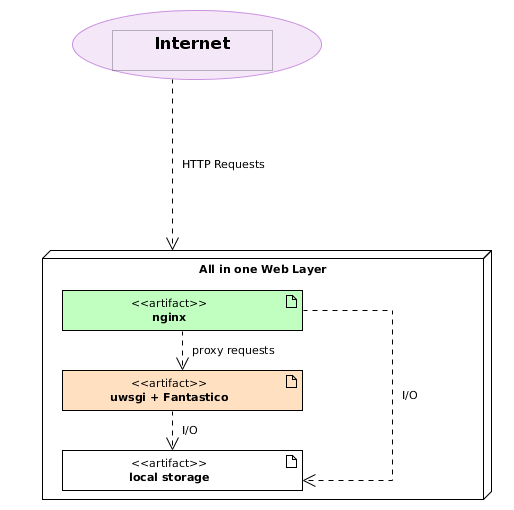
\includegraphics{low_usage_all_in_one.png}

Above diagram described the simplest scenario for rolling out Fantastico to production. You can use this scenario
for minimalistic web applications like:
\begin{itemize}
\item {} 
Presentation website

\item {} 
Personal website

\item {} 
Blog

\end{itemize}

We usually recommend to start with this deployment scenario and the migrate to more complex scenarios when
you application requires it.

\begin{tabulary}{\linewidth}{|L|L|}
\hline
\textbf{\relax 
Advantages
} & \textbf{\relax 
Disadvantages
}\\\hline

Extremely easy to deploy
 & 
Does not scale well for more than couple of requests / second
\\\hline

Minimal os configuration
 & 
All components are bundled on one node without any failover.
\\\hline

Automatic scripts for configuring the os
 & 
Does not support vertical scaling out of the box.
\\\hline

Easy to achieve horizontal scaling for all components at once.
 & 
Static files are not served from a cdn.
\\\hline
\end{tabulary}



\subsubsection{Setup}
\label{how_to/deployment/low_usage_scenario:setup}\begin{enumerate}
\item {} 
Install Fantastico framework on the production machine ({\hyperref[get_started/installation::doc]{\emph{Installation manual}}}.).

\item {} 
Goto \$FANTASTICO\_ROOT

\item {} 
export ROOT\_PASSWD=\textless{}your root password\textgreater{}

\item {} 
fantastico\_setup\_low\_usage\_\textless{}os\_distribution) --ipaddress \textless{}desired\_ip\textgreater{} --vhost-name \textless{}desired\_vhost\textgreater{} --uwsgi-port \textless{}uwsgi port\textgreater{} --root-folder \textless{}desired root folder\textgreater{} --modules-folder \textless{}desired modules folder\textgreater{} (e.g fantastico\_setup\_low\_usage\_ubuntu.sh --ipaddress 127.0.0.1 --vhost-name fantastico-framework.com --uwsgi-port 12090 --root-folder {}`pwd{}` --modules-folder /fantastico/samples)

\item {} 
Done.

\end{enumerate}

It is usually a good idea to change the number of parallel connections supported by your linux kernel:
\begin{enumerate}
\item {} 
sudo nano /etc/sysctl.conf

\item {} 
Search for \textbf{net.core.somaxconn}.

\item {} 
If it does not exist you can add net.core.somaxconn = 8192 to the bottom of the file.

\item {} 
Restart the os.

\end{enumerate}


\subsection{Low usage AWS}
\label{how_to/deployment/aws_low_usage_scenario:low-usage-aws}\label{how_to/deployment/aws_low_usage_scenario::doc}
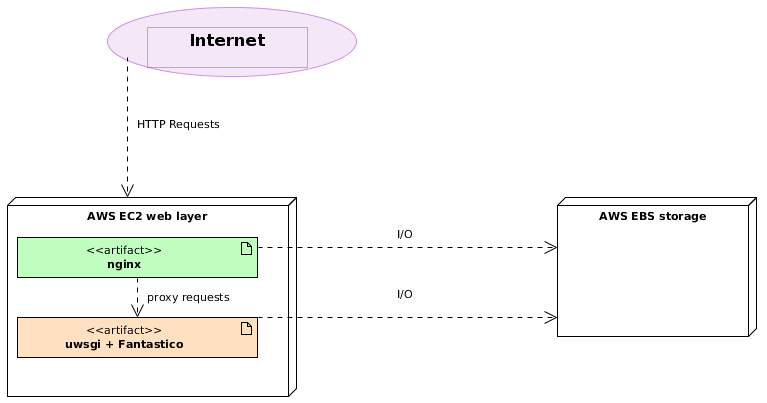
\includegraphics{low_usage_aws.png}

This scenario is a little bit more complex than {\hyperref[how_to/deployment/low_usage_scenario::doc]{\emph{Low usage (simplest scenario)}}} but it provides some
advantages:

\begin{tabulary}{\linewidth}{|L|L|}
\hline
\textbf{\relax 
Advantages
} & \textbf{\relax 
Disadvantages
}\\\hline

Can be autoscaled.
 & 
Requires AWS EC2 instances
\\\hline

Easier crash recovery
 & 
Requires manual configuration
\\\hline

Very easy monitoring support (CloudWatch)
 & 
Requires AWS EBS.
\\\hline
 & 
Requires some AWS know how.
\\\hline
 & 
Static files are not served from a cdn.
\\\hline
\end{tabulary}


This scenario is recommended if you want to rollout you application on AWS infrastructure. Usually it is non expensive
to do this as it requires micro instances and low cost storage. For more information about AWS required components
read:
\begin{enumerate}
\item {} 
\href{http://aws.amazon.com/ec2/instance-types/}{AWS Instance types}.

\item {} 
\href{http://aws.amazon.com/ebs/}{AWS EBS}.

\end{enumerate}


\subsubsection{Setup}
\label{how_to/deployment/aws_low_usage_scenario:setup}\begin{enumerate}
\item {} 
Create an AWS account. (\href{http://aws.amazon.com/documentation/gettingstarted/}{AWS Getting Started}).

\item {} 
Create an EC2 instance from AWS Management Console (\href{http://www.youtube.com/watch?v=WBro0TEAd7g}{EC2 setup}).

\item {} 
SSH on EC2 instance.

\item {} 
Install Fantastico framework on the production machine ({\hyperref[get_started/installation::doc]{\emph{Installation manual}}}.).

\item {} 
Goto \$FANTASTICO\_ROOT

\item {} 
fantastico\_setup\_low\_usage\_\textless{}os\_distribution).sh (e.g fantastico\_setup\_low\_usage\_ubuntu.sh)

\item {} 
Done.

\end{enumerate}


\subsubsection{Optimization}
\label{how_to/deployment/aws_low_usage_scenario:optimization}
This scenario can be easily optimized by using \textbf{AWS S3} buckets for static files. This ensures faileover for static
files and very easy horizontal scaling for sites. Below you can find the new diagram:

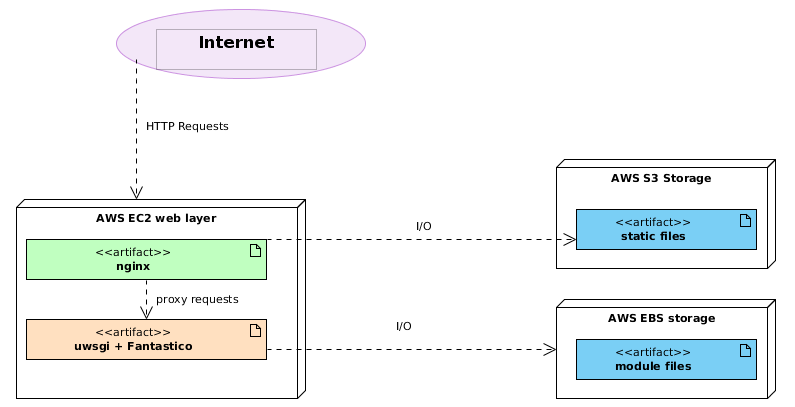
\includegraphics{low_usage_s3_aws.png}

You can read more about \textbf{AWS S3} storage on \href{http://aws.amazon.com/s3/}{http://aws.amazon.com/s3/}. In this version of fantastico there is no
way to sync static module files with S3 buckets. This feature is going to be implemented in upcoming \textbf{Fantastico}
features. As a workaround you can easily copy \textbf{static} folder content from each module on S3 using the tool
provided from AWS Management Console.

You can see how to use AWS Management Console S3 tool on \href{http://www.youtube.com/watch?v=1qrjFb0ZTm8}{http://www.youtube.com/watch?v=1qrjFb0ZTm8}


\subsubsection{Setup with S3}
\label{how_to/deployment/aws_low_usage_scenario:setup-with-s3}\begin{enumerate}
\item {} 
export ROOT\_PASSWD=\textless{}your root password\textgreater{}

\item {} 
Create an AWS account. (\href{http://aws.amazon.com/documentation/gettingstarted/}{AWS Getting Started}).

\item {} 
Create an EC2 instance from AWS Management Console (\href{http://www.youtube.com/watch?v=WBro0TEAd7g}{EC2 setup}).

\item {} 
SSH on EC2 instance.

\item {} 
Install Fantastico framework on the production machine ({\hyperref[get_started/installation::doc]{\emph{Installation manual}}}.).

\item {} 
Goto \$FANTASTICO\_ROOT/deployment

\item {} 
fantastico\_setup\_low\_usage\_s3\_\textless{}os\_distribution).sh --ipaddress \textless{}desired\_ip\textgreater{} --vhost-name \textless{}desired\_vhost\textgreater{} --uwsgi-port \textless{}uwsgi port\textgreater{} --root-folder \textless{}desired root folder\textgreater{} --modules-folder \textless{}desired modules folder\textgreater{} (e.g fantastico\_setup\_low\_usage\_s3\_ubuntu.sh --ipaddress 127.0.0.1 --vhost-name fantastico-framework.com --uwsgi-port 12090 --root-folder {}`pwd{}` --modules-folder /fantastico/samples)

\item {} 
Done.

\end{enumerate}

It is usually a good idea to change the number of parallel connections supported by your linux kernel:
\begin{enumerate}
\item {} 
sudo nano /etc/sysctl.conf

\item {} 
Search for \textbf{net.core.somaxconn}.

\item {} 
If it does not exist you can add net.core.somaxconn = 8192 to the bottom of the file.

\item {} 
Restart the os.

\end{enumerate}


\section{Static assets}
\label{how_to/static_assets:static-assets}\label{how_to/static_assets::doc}
By default, static assets can be any file that is publicly available. Most of the time, here you can place:
\begin{itemize}
\item {} 
css files

\item {} 
png, jpg, gif files

\item {} 
downloadable pdf

\item {} 
movie files

\item {} 
any other file format you can think about

\end{itemize}

For Production environment, requests to these files are handled by the web server you are using. You only need to
place them under \textbf{static} folder of your component ({\hyperref[features/component_model::doc]{\emph{Component model}}}).

There are several scenario in which Fantastico projects are deployed which influence where your component static files
are stored. I recommend you read {\hyperref[how_to/deployment_how_to::doc]{\emph{Deployment how to}}} section.


\subsection{Static assets on dev}
\label{how_to/static_assets:static-assets-on-dev}
Of course, on development environment you are not required to have a web server in front of your Fantastico dev server.
For this purpose, fantastico framework provides a special controller which can easily serve static files. Even though
it works as expected, please do not use it in production. It does not send headers required by browser for caching
purposes.

Static assets routes are the same between \textbf{prod} and \textbf{dev} environments.


\subsubsection{Favicon}
\label{how_to/static_assets:favicon}
If you want your site to also have an icon which is automatically presented by browsers, in your project root folder
do the following:
\begin{enumerate}
\item {} 
mkdir static

\item {} 
cd static

\item {} 
Copy your favicon.ico file in here.

\end{enumerate}


\subsection{Static assets on prod}
\label{how_to/static_assets:static-assets-on-prod}
There is no difference between static assets on dev and static assets on production from routes point of view.
From handling requests point of view, nginx configuration for your project takes care of serving static assets
and sending correct http caching headers.


\chapter{Fantastico features}
\label{features/features::doc}\label{features/features:fantastico-features}

\section{Exceptions hierarchy}
\label{features/exceptions:exceptions-hierarchy}\label{features/exceptions::doc}\index{FantasticoError (class in fantastico.exceptions)}

\begin{fulllineitems}
\phantomsection\label{features/exceptions:fantastico.exceptions.FantasticoError}\pysiglinewithargsret{\strong{class }\code{fantastico.exceptions.}\bfcode{FantasticoError}}{\emph{msg=None}, \emph{http\_code=400}}{}~
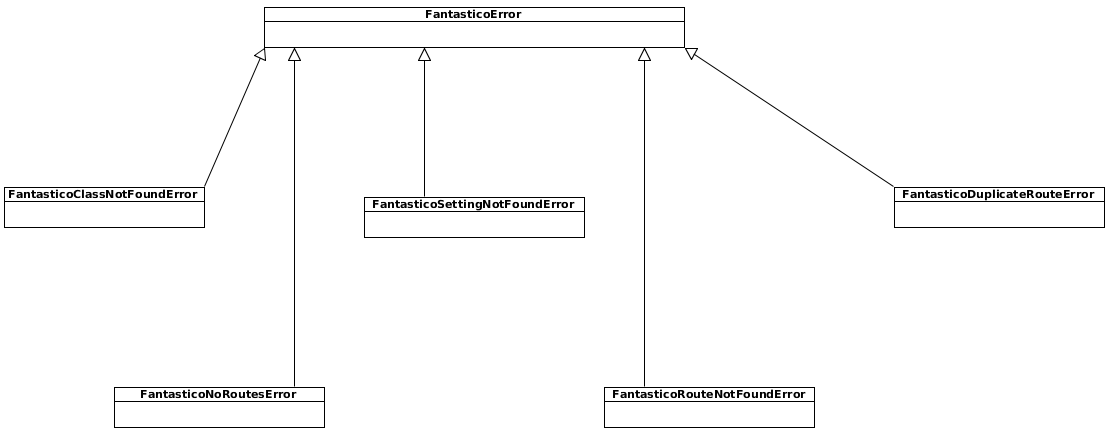
\includegraphics{exceptions.png}

\textbf{FantasticoError} is the base of all exceptions raised within fantastico framework. It describe common attributes that
each concrete fantastico exception must provide. By default all fantastico exceptions inherit FantasticoError exception.
We do this because each raised unhandled FantasticoError is map to a specific exception response. This strategy guarantees
that at no moment errors will cause fantastico framework wsgi container to crash.
\index{http\_code (fantastico.exceptions.FantasticoError attribute)}

\begin{fulllineitems}
\phantomsection\label{features/exceptions:fantastico.exceptions.FantasticoError.http_code}\pysigline{\bfcode{http\_code}}
This method returns the http code on which this exception is mapped.

\end{fulllineitems}


\end{fulllineitems}

\index{FantasticoControllerInvalidError (class in fantastico.exceptions)}

\begin{fulllineitems}
\phantomsection\label{features/exceptions:fantastico.exceptions.FantasticoControllerInvalidError}\pysiglinewithargsret{\strong{class }\code{fantastico.exceptions.}\bfcode{FantasticoControllerInvalidError}}{\emph{msg=None}, \emph{http\_code=400}}{}
This exception is raised whenever a method is decorated with
{\hyperref[features/mvc:fantastico.mvc.controller_decorators.Controller]{\code{fantastico.mvc.controller\_decorators.Controller}}} and the number of arguments is not correct. Usually
developer forgot to add request as argument to the controller.

\end{fulllineitems}

\index{FantasticoClassNotFoundError (class in fantastico.exceptions)}

\begin{fulllineitems}
\phantomsection\label{features/exceptions:fantastico.exceptions.FantasticoClassNotFoundError}\pysiglinewithargsret{\strong{class }\code{fantastico.exceptions.}\bfcode{FantasticoClassNotFoundError}}{\emph{msg=None}, \emph{http\_code=400}}{}
This exception is raised whenever code tries to dynamically import and instantiate a class which can not be resolved.

\end{fulllineitems}

\index{FantasticoNotSupportedError (class in fantastico.exceptions)}

\begin{fulllineitems}
\phantomsection\label{features/exceptions:fantastico.exceptions.FantasticoNotSupportedError}\pysiglinewithargsret{\strong{class }\code{fantastico.exceptions.}\bfcode{FantasticoNotSupportedError}}{\emph{msg=None}, \emph{http\_code=400}}{}
This exception is raised whenever code tries to do an operation that is  not supported.

\end{fulllineitems}

\index{FantasticoSettingNotFoundError (class in fantastico.exceptions)}

\begin{fulllineitems}
\phantomsection\label{features/exceptions:fantastico.exceptions.FantasticoSettingNotFoundError}\pysiglinewithargsret{\strong{class }\code{fantastico.exceptions.}\bfcode{FantasticoSettingNotFoundError}}{\emph{msg=None}, \emph{http\_code=400}}{}
This exception is raised whenever code tries to obtain a setting that is not available in the current fantastico
configuration.

\end{fulllineitems}

\index{FantasticoDuplicateRouteError (class in fantastico.exceptions)}

\begin{fulllineitems}
\phantomsection\label{features/exceptions:fantastico.exceptions.FantasticoDuplicateRouteError}\pysiglinewithargsret{\strong{class }\code{fantastico.exceptions.}\bfcode{FantasticoDuplicateRouteError}}{\emph{msg=None}, \emph{http\_code=400}}{}
This exception is usually raised by routing engine when it detects duplicate routes.

\end{fulllineitems}

\index{FantasticoNoRoutesError (class in fantastico.exceptions)}

\begin{fulllineitems}
\phantomsection\label{features/exceptions:fantastico.exceptions.FantasticoNoRoutesError}\pysiglinewithargsret{\strong{class }\code{fantastico.exceptions.}\bfcode{FantasticoNoRoutesError}}{\emph{msg=None}, \emph{http\_code=400}}{}
This exception is usually raised by routing engine when no loaders are configured or no routes are registered.

\end{fulllineitems}

\index{FantasticoRouteNotFoundError (class in fantastico.exceptions)}

\begin{fulllineitems}
\phantomsection\label{features/exceptions:fantastico.exceptions.FantasticoRouteNotFoundError}\pysiglinewithargsret{\strong{class }\code{fantastico.exceptions.}\bfcode{FantasticoRouteNotFoundError}}{\emph{msg=None}, \emph{http\_code=400}}{}
This exception is usually raised by routing engine when a requested url is not registered.

\end{fulllineitems}

\index{FantasticoNoRequestError (class in fantastico.exceptions)}

\begin{fulllineitems}
\phantomsection\label{features/exceptions:fantastico.exceptions.FantasticoNoRequestError}\pysiglinewithargsret{\strong{class }\code{fantastico.exceptions.}\bfcode{FantasticoNoRequestError}}{\emph{msg=None}, \emph{http\_code=400}}{}
This exception is usually raised when some components try to use fantastico.request from WSGI environ before
{\hyperref[features/request_response:fantastico.middleware.request_middleware.RequestMiddleware]{\code{fantastico.middleware.request\_middleware.RequestMiddleware}}} was executed.

\end{fulllineitems}

\index{FantasticoContentTypeError (class in fantastico.exceptions)}

\begin{fulllineitems}
\phantomsection\label{features/exceptions:fantastico.exceptions.FantasticoContentTypeError}\pysiglinewithargsret{\strong{class }\code{fantastico.exceptions.}\bfcode{FantasticoContentTypeError}}{\emph{msg=None}, \emph{http\_code=400}}{}
This exception is usually thrown when a mismatch between request accept and response content type. In
Fantastico we think it's mandatory to fulfill requests correctly and to take in consideration sent headers.

\end{fulllineitems}

\index{FantasticoHttpVerbNotSupported (class in fantastico.exceptions)}

\begin{fulllineitems}
\phantomsection\label{features/exceptions:fantastico.exceptions.FantasticoHttpVerbNotSupported}\pysiglinewithargsret{\strong{class }\code{fantastico.exceptions.}\bfcode{FantasticoHttpVerbNotSupported}}{\emph{http\_verb}}{}
This exception is usually thrown when a route is accessed with an http verb which does not support.
\index{http\_verb (fantastico.exceptions.FantasticoHttpVerbNotSupported attribute)}

\begin{fulllineitems}
\phantomsection\label{features/exceptions:fantastico.exceptions.FantasticoHttpVerbNotSupported.http_verb}\pysigline{\bfcode{http\_verb}}
This property returns the http verb that caused the problems.

\end{fulllineitems}


\end{fulllineitems}

\index{FantasticoTemplateNotFoundError (class in fantastico.exceptions)}

\begin{fulllineitems}
\phantomsection\label{features/exceptions:fantastico.exceptions.FantasticoTemplateNotFoundError}\pysiglinewithargsret{\strong{class }\code{fantastico.exceptions.}\bfcode{FantasticoTemplateNotFoundError}}{\emph{msg=None}, \emph{http\_code=400}}{}
This exception is usually thrown when a controller tries to load a template which it does not found.

\end{fulllineitems}

\index{FantasticoIncompatibleClassError (class in fantastico.exceptions)}

\begin{fulllineitems}
\phantomsection\label{features/exceptions:fantastico.exceptions.FantasticoIncompatibleClassError}\pysiglinewithargsret{\strong{class }\code{fantastico.exceptions.}\bfcode{FantasticoIncompatibleClassError}}{\emph{msg=None}, \emph{http\_code=400}}{}
This exception is usually thrown when we want to decorate / inject / mixin a class into another class
that does not support it. For instance, we want to build a {\hyperref[features/mvc:fantastico.mvc.model_facade.ModelFacade]{\code{fantastico.mvc.model\_facade.ModelFacade}}}
with a class that does not extend \textbf{BASEMODEL.}

\end{fulllineitems}

\index{FantasticoDbError (class in fantastico.exceptions)}

\begin{fulllineitems}
\phantomsection\label{features/exceptions:fantastico.exceptions.FantasticoDbError}\pysiglinewithargsret{\strong{class }\code{fantastico.exceptions.}\bfcode{FantasticoDbError}}{\emph{msg=None}, \emph{http\_code=400}}{}
This exception is usually thrown when a database exception occurs. For one good example where this is used see
{\hyperref[features/mvc:fantastico.mvc.model_facade.ModelFacade]{\code{fantastico.mvc.model\_facade.ModelFacade}}}.

\end{fulllineitems}

\index{FantasticoDbNotFoundError (class in fantastico.exceptions)}

\begin{fulllineitems}
\phantomsection\label{features/exceptions:fantastico.exceptions.FantasticoDbNotFoundError}\pysiglinewithargsret{\strong{class }\code{fantastico.exceptions.}\bfcode{FantasticoDbNotFoundError}}{\emph{msg=None}, \emph{http\_code=400}}{}
This exception is usually thrown when an entity does not exist but we try to update it. For one good example where this is
used see {\hyperref[features/mvc:fantastico.mvc.model_facade.ModelFacade]{\code{fantastico.mvc.model\_facade.ModelFacade}}}.

\end{fulllineitems}

\index{FantasticoInsufficientArgumentsError (class in fantastico.exceptions)}

\begin{fulllineitems}
\phantomsection\label{features/exceptions:fantastico.exceptions.FantasticoInsufficientArgumentsError}\pysiglinewithargsret{\strong{class }\code{fantastico.exceptions.}\bfcode{FantasticoInsufficientArgumentsError}}{\emph{msg=None}, \emph{http\_code=400}}{}
This exception is usually thrown when a component extension received wrong number of arguments. See
{\hyperref[features/component_reusage:fantastico.rendering.component.Component]{\code{fantastico.rendering.component.Component}}}.

\end{fulllineitems}

\index{FantasticoUrlInvokerError (class in fantastico.exceptions)}

\begin{fulllineitems}
\phantomsection\label{features/exceptions:fantastico.exceptions.FantasticoUrlInvokerError}\pysiglinewithargsret{\strong{class }\code{fantastico.exceptions.}\bfcode{FantasticoUrlInvokerError}}{\emph{msg=None}, \emph{http\_code=400}}{}
This exception is usually thrown when an internal url invoker fails. For instance, if a component reusage rendering
fails then this exception is raised.

\end{fulllineitems}



\section{Request lifecycle}
\label{features/request_response:request-lifecycle}\label{features/request_response::doc}
In this document you can find how a request is processed by fantastico framework. By default WSGI applications use a dictionary
that contains various useful keys:
\begin{itemize}
\item {} 
HTTP Headers

\item {} 
HTTP Cookies

\item {} 
Helper keys (e.g file wrapper).

\end{itemize}

In fantastico we want to hide the complexity of this dictionary and allow developers to use some standardized objects. Fantastico
framework follows a Request / Response paradigm. This mean that for every single http request only one single http response will
be generated. Below, you can find a simple example of how requests are processed by fantastico framework:

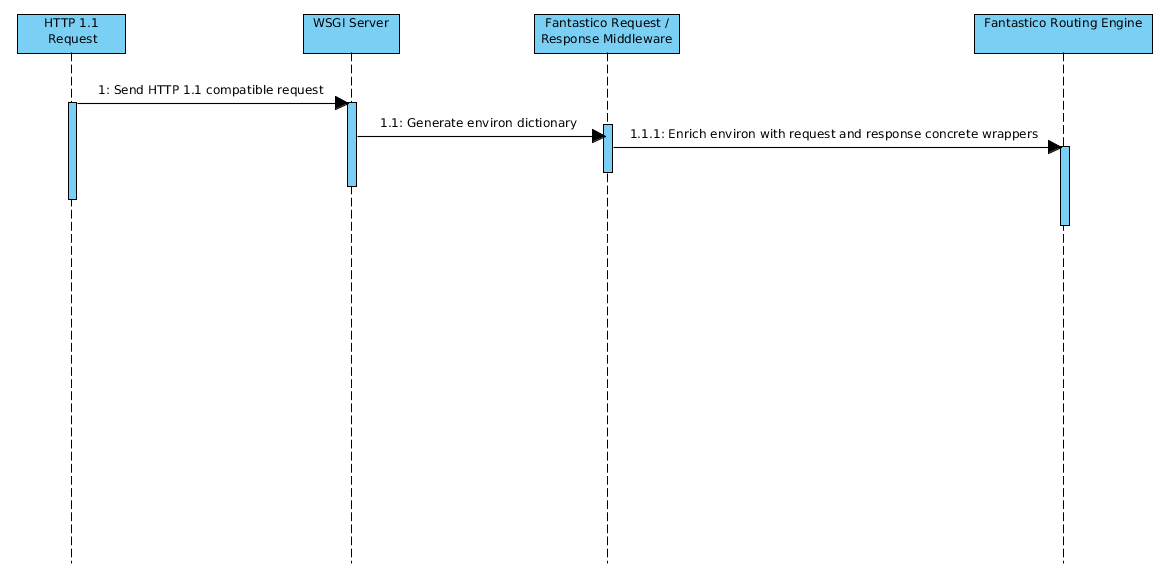
\includegraphics{request_response_sd.png}

In order to not reinvent the wheels fantastico relies on WebOb python framework in order to correctly generate request and
response objects. For more information read \href{http://docs.webob.org/en/latest/reference.html}{WebOB Doc}.


\subsection{Request middleware}
\label{features/request_response:request-middleware}
To have very good control of how WSGI environ is wrapped into \textbf{WebOb request} object a middleware component is configured. This
is the first middleware that is executed for every single http request.
\index{RequestMiddleware (class in fantastico.middleware.request\_middleware)}

\begin{fulllineitems}
\phantomsection\label{features/request_response:fantastico.middleware.request_middleware.RequestMiddleware}\pysiglinewithargsret{\strong{class }\code{fantastico.middleware.request\_middleware.}\bfcode{RequestMiddleware}}{\emph{app}}{}
This class provides the middleware responsible for converting wsgi environ dictionary into a request. The result is saved
into current WSGI environ under key \textbf{fantastico.request}. In addition each new request receives an identifier. If subsequent
requests are triggered from that request then they will also receive the same request id.

\end{fulllineitems}



\subsection{Request context}
\label{features/request_response:request-context}
In comparison with WebOb \textbf{Fantastico} provides a nice improvement. For facilitating easy development of code, each fantastico
request has a special attribute called context. Below you can find the attributes of a request context object:
\begin{itemize}
\item {} 
settings facade ({\hyperref[get_started/settings::doc]{\emph{Fantastico settings}}})

\item {} 
session (not yet supported)

\item {} 
\textbf{language} The current preferred by user. This is determined based on user lang header.

\item {} 
user (not yet supported)

\end{itemize}
\index{RequestContext (class in fantastico.middleware.request\_context)}

\begin{fulllineitems}
\phantomsection\label{features/request_response:fantastico.middleware.request_context.RequestContext}\pysiglinewithargsret{\strong{class }\code{fantastico.middleware.request\_context.}\bfcode{RequestContext}}{\emph{settings}, \emph{language}}{}
This class holds various attributes useful giving a context to an http request. Among other things we need
to be able to access current language, current session and possible current user profile.
\index{language (fantastico.middleware.request\_context.RequestContext attribute)}

\begin{fulllineitems}
\phantomsection\label{features/request_response:fantastico.middleware.request_context.RequestContext.language}\pysigline{\bfcode{language}}
Property that holds the current language that must be used during this request.

\end{fulllineitems}

\index{settings (fantastico.middleware.request\_context.RequestContext attribute)}

\begin{fulllineitems}
\phantomsection\label{features/request_response:fantastico.middleware.request_context.RequestContext.settings}\pysigline{\bfcode{settings}}
Property that holds the current settings facade used for accessing fantastico configuration.

\end{fulllineitems}

\index{wsgi\_app (fantastico.middleware.request\_context.RequestContext attribute)}

\begin{fulllineitems}
\phantomsection\label{features/request_response:fantastico.middleware.request_context.RequestContext.wsgi_app}\pysigline{\bfcode{wsgi\_app}}
Property that holds the WSGI application instance under which the request is handled.

\end{fulllineitems}


\end{fulllineitems}



\subsection{Obtain request language}
\label{features/request_response:obtain-request-language}\index{Language (class in fantastico.locale.language)}

\begin{fulllineitems}
\phantomsection\label{features/request_response:fantastico.locale.language.Language}\pysiglinewithargsret{\strong{class }\code{fantastico.locale.language.}\bfcode{Language}}{\emph{code}}{}
Class used to define how does language object looks like. There are various use cases for using language but
the simplest one is in request context object:

\begin{Verbatim}[commandchars=\\\{\}]
\PYG{n}{language} \PYG{o}{=} \PYG{n}{request}\PYG{o}{.}\PYG{n}{context}\PYG{o}{.}\PYG{n}{language}

\PYG{k}{if} \PYG{n}{language}\PYG{o}{.}\PYG{n}{code} \PYG{o}{=} \PYG{l+s}{\PYGZdq{}}\PYG{l+s}{en\PYGZus{}us}\PYG{l+s}{\PYGZdq{}}\PYG{p}{:}
   \PYG{k}{print}\PYG{p}{(}\PYG{l+s}{\PYGZdq{}}\PYG{l+s}{English (US) language}\PYG{l+s}{\PYGZdq{}}\PYG{p}{)}\PYG{o}{.}
\PYG{k}{else}\PYG{p}{:}
   \PYG{k}{raise} \PYG{n+ne}{Exception}\PYG{p}{(}\PYG{l+s}{\PYGZdq{}}\PYG{l+s}{Language }\PYG{l+s+si}{\PYGZpc{}s}\PYG{l+s}{ is not supported.}\PYG{l+s}{\PYGZdq{}} \PYG{o}{\PYGZpc{}} \PYG{n}{language}\PYG{o}{.}\PYG{n}{code}\PYG{p}{)}
\end{Verbatim}
\index{code (fantastico.locale.language.Language attribute)}

\begin{fulllineitems}
\phantomsection\label{features/request_response:fantastico.locale.language.Language.code}\pysigline{\bfcode{code}}
Property that holds the language code. This is readonly because once instantiated we mustn't be able to change it.

\end{fulllineitems}


\end{fulllineitems}



\subsection{Obtain settings using request}
\label{features/request_response:obtain-settings-using-request}
It is recommended to use \emph{request.context} object to obtain fantastico settings. This hides the complexity of choosing the right
configuration and accessing attributes from it.

\begin{Verbatim}[commandchars=\\\{\}]
\PYG{n}{installed\PYGZus{}middleware} \PYG{o}{=} \PYG{n}{request}\PYG{o}{.}\PYG{n}{context}\PYG{o}{.}\PYG{n}{settings}\PYG{o}{.}\PYG{n}{get}\PYG{p}{(}\PYG{l+s}{\PYGZdq{}}\PYG{l+s}{installed\PYGZus{}middleware}\PYG{l+s}{\PYGZdq{}}\PYG{p}{)}

\PYG{k}{print}\PYG{p}{(}\PYG{n}{installed\PYGZus{}middleware}\PYG{p}{)}
\end{Verbatim}

For more information about how to configure \textbf{Fantastico} please read {\hyperref[get_started/settings::doc]{\emph{Fantastico settings}}}.


\subsection{Redirect using request}
\label{features/request_response:redirect-using-request}
In Fantastico is fairly simply to redirect client to a given location.
\index{RedirectResponse (class in fantastico.routing\_engine.custom\_responses)}

\begin{fulllineitems}
\phantomsection\label{features/request_response:fantastico.routing_engine.custom_responses.RedirectResponse}\pysiglinewithargsret{\strong{class }\code{fantastico.routing\_engine.custom\_responses.}\bfcode{RedirectResponse}}{\emph{destination}, \emph{query\_params=None}, \emph{redirect\_status=302}}{}
This class encapsulates the logic for programatically redirecting client from a fantastico controller.

\begin{Verbatim}[commandchars=\\\{\}]
\PYG{n+nd}{@Controller}\PYG{p}{(}\PYG{n}{url}\PYG{o}{=}\PYG{l+s}{\PYGZdq{}}\PYG{l+s}{/redirect/example}\PYG{l+s}{\PYGZdq{}}\PYG{p}{)}
\PYG{k}{def} \PYG{n+nf}{redirect\PYGZus{}to\PYGZus{}google}\PYG{p}{(}\PYG{n+nb+bp}{self}\PYG{p}{,} \PYG{n}{request}\PYG{p}{)}\PYG{p}{:}
    \PYG{k}{return} \PYG{n}{request}\PYG{o}{.}\PYG{n}{redirect}\PYG{p}{(}\PYG{l+s}{\PYGZdq{}}\PYG{l+s}{http://www.google.ro/}\PYG{l+s}{\PYGZdq{}}\PYG{p}{)}
\end{Verbatim}

There are some special cases when you would like to pass some query parameters to redirect destination. This is also easily
achievable in Fantastico:

\begin{Verbatim}[commandchars=\\\{\}]
\PYG{n+nd}{@Controller}\PYG{p}{(}\PYG{n}{url}\PYG{o}{=}\PYG{l+s}{\PYGZdq{}}\PYG{l+s}{/redirect/example}\PYG{l+s}{\PYGZdq{}}\PYG{p}{)}
\PYG{k}{def} \PYG{n+nf}{redirect\PYGZus{}to\PYGZus{}google}\PYG{p}{(}\PYG{n+nb+bp}{self}\PYG{p}{,} \PYG{n}{request}\PYG{p}{)}\PYG{p}{:}
    \PYG{k}{return} \PYG{n}{request}\PYG{o}{.}\PYG{n}{redirect}\PYG{p}{(}\PYG{l+s}{\PYGZdq{}}\PYG{l+s}{http://www.google.ro/search}\PYG{l+s}{\PYGZdq{}}\PYG{p}{,}
                            \PYG{n}{query\PYGZus{}params}\PYG{o}{=}\PYG{p}{[}\PYG{p}{(}\PYG{l+s}{\PYGZdq{}}\PYG{l+s}{q}\PYG{l+s}{\PYGZdq{}}\PYG{p}{,} \PYG{l+s}{\PYGZdq{}}\PYG{l+s}{hello world}\PYG{l+s}{\PYGZdq{}}\PYG{p}{)}\PYG{p}{]}\PYG{p}{)}
\end{Verbatim}

The above example will redirect client browser to
\href{http://www.google.ro/search?q=helloworld}{http://www.google.ro/search?q=hello world}

\end{fulllineitems}



\section{Routing engine}
\label{features/routing_engine:routing-engine}\label{features/routing_engine::doc}
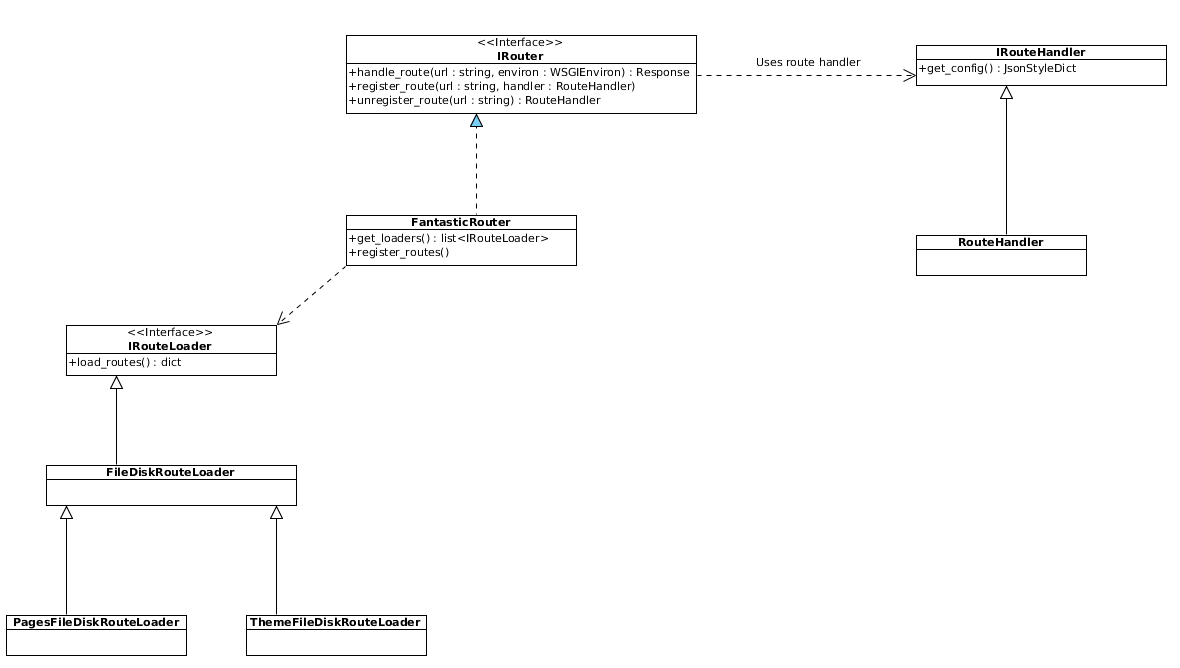
\includegraphics{routing_engine.png}

Fantastico routing engine is design by having extensibility in mind. Below you can find the list of concerns for routing engine:
\begin{enumerate}
\item {} 
Support multiple sources for routes.

\item {} 
Load all available routes.

\item {} 
Select the controller that can handle the request route (if any available).

\end{enumerate}
\index{Router (class in fantastico.routing\_engine.router)}

\begin{fulllineitems}
\phantomsection\label{features/routing_engine:fantastico.routing_engine.router.Router}\pysiglinewithargsret{\strong{class }\code{fantastico.routing\_engine.router.}\bfcode{Router}}{\emph{settings\_facade=\textless{}class `fantastico.settings.SettingsFacade'\textgreater{}}}{}
This class is used for registering all available routes by using all registered loaders.
\index{get\_loaders() (fantastico.routing\_engine.router.Router method)}

\begin{fulllineitems}
\phantomsection\label{features/routing_engine:fantastico.routing_engine.router.Router.get_loaders}\pysiglinewithargsret{\bfcode{get\_loaders}}{}{}
Method used to retrieve all available loaders. If loaders are not currently instantiated they are by these method.
This method also supports multi threaded workers mode of wsgi with really small memory footprint. It uses an internal
lock so that it makes sure available loaders are instantiated only once per wsgi worker.

\end{fulllineitems}

\index{handle\_route() (fantastico.routing\_engine.router.Router method)}

\begin{fulllineitems}
\phantomsection\label{features/routing_engine:fantastico.routing_engine.router.Router.handle_route}\pysiglinewithargsret{\bfcode{handle\_route}}{\emph{url}, \emph{environ}}{}
Method used to identify the given url method handler. It enrich the environ dictionary with a new entry that
holds a controller instance and a function to be executed from that controller.

\end{fulllineitems}

\index{register\_routes() (fantastico.routing\_engine.router.Router method)}

\begin{fulllineitems}
\phantomsection\label{features/routing_engine:fantastico.routing_engine.router.Router.register_routes}\pysiglinewithargsret{\bfcode{register\_routes}}{}{}
Method used to register all routes from all loaders. If the loaders are not yet initialized this method will first
load all available loaders and then it will register all available routes. Also, this method initialize available routes
only once when it is first invoked.

\end{fulllineitems}


\end{fulllineitems}



\subsection{Routes loaders}
\label{features/routing_engine:routes-loaders}
Fantastico routing engine is designed so that routes can be loaded from multiple sources (database, disk locations, and others).
This give huge extensibility so that developers can use Fantastico in various scenarios:
\begin{itemize}
\item {} 
Create a CMS that allows people to create new pages (mapping between page url / controller) is hold in database. Just by
adding a simple loader in which the business logic is encapsulated allows routing engine extension.

\item {} 
Create a blog that loads articles from disk.

\end{itemize}

I am sure you can find other use cases in which you benefit from this extension point.


\subsection{How to write a new route loader}
\label{features/routing_engine:how-to-write-a-new-route-loader}
Before digging in further details see the RouteLoader class documentation below:
\index{RouteLoader (class in fantastico.routing\_engine.routing\_loaders)}

\begin{fulllineitems}
\phantomsection\label{features/routing_engine:fantastico.routing_engine.routing_loaders.RouteLoader}\pysiglinewithargsret{\strong{class }\code{fantastico.routing\_engine.routing\_loaders.}\bfcode{RouteLoader}}{\emph{settings\_facade}}{}
This class provides the contract that must be provided by each concrete implementation. Each route loader is responsible
for implementing its own business logic for loading routes.

\begin{Verbatim}[commandchars=\\\{\}]
\PYG{k}{class} \PYG{n+nc}{DummyRouteLoader}\PYG{p}{(}\PYG{n}{RouteLoader}\PYG{p}{)}\PYG{p}{:}
    \PYG{k}{def} \PYG{n+nf}{\PYGZus{}\PYGZus{}init\PYGZus{}\PYGZus{}}\PYG{p}{(}\PYG{n+nb+bp}{self}\PYG{p}{,} \PYG{n}{settings\PYGZus{}facade}\PYG{p}{)}\PYG{p}{:}
        \PYG{n}{self\PYGZus{}settings\PYGZus{}facade} \PYG{o}{=} \PYG{n}{settings\PYGZus{}facade}

    \PYG{k}{def} \PYG{n+nf}{load\PYGZus{}routes}\PYG{p}{(}\PYG{n+nb+bp}{self}\PYG{p}{)}\PYG{p}{:}
        \PYG{k}{return} \PYG{p}{\PYGZob{}}\PYG{l+s}{\PYGZdq{}}\PYG{l+s}{/index.html}\PYG{l+s}{\PYGZdq{}}\PYG{p}{:} \PYG{p}{\PYGZob{}}\PYG{l+s}{\PYGZdq{}}\PYG{l+s}{http\PYGZus{}verbs}\PYG{l+s}{\PYGZdq{}}\PYG{p}{:} \PYG{p}{\PYGZob{}}
                                            \PYG{l+s}{\PYGZdq{}}\PYG{l+s}{GET}\PYG{l+s}{\PYGZdq{}}\PYG{p}{:} \PYG{l+s}{\PYGZdq{}}\PYG{l+s}{fantastico.plugins.static\PYGZus{}assets.StaticAssetsController.resolve\PYGZus{}text}\PYG{l+s}{\PYGZdq{}}
                                            \PYG{p}{\PYGZcb{}}
                                \PYG{p}{\PYGZcb{}}\PYG{p}{,}
                \PYG{l+s}{\PYGZdq{}}\PYG{l+s}{/images/image.png}\PYG{l+s}{\PYGZdq{}}\PYG{p}{:} \PYG{p}{\PYGZob{}}\PYG{l+s}{\PYGZdq{}}\PYG{l+s}{http\PYGZus{}verbs}\PYG{l+s}{\PYGZdq{}}\PYG{p}{:} \PYG{p}{\PYGZob{}}
                                            \PYG{l+s}{\PYGZdq{}}\PYG{l+s}{GET}\PYG{l+s}{\PYGZdq{}}\PYG{p}{:} \PYG{l+s}{\PYGZdq{}}\PYG{l+s}{fantastico.plugins.static\PYGZus{}assets.StaticAssetsController.resolve\PYGZus{}binary}\PYG{l+s}{\PYGZdq{}}
                                            \PYG{p}{\PYGZcb{}}
                                     \PYG{p}{\PYGZcb{}}
        \PYG{p}{\PYGZcb{}}
\end{Verbatim}
\index{load\_routes() (fantastico.routing\_engine.routing\_loaders.RouteLoader method)}

\begin{fulllineitems}
\phantomsection\label{features/routing_engine:fantastico.routing_engine.routing_loaders.RouteLoader.load_routes}\pysiglinewithargsret{\bfcode{load\_routes}}{}{}
This method must be overriden by each concrete implementation so that all loaded routes can be handled by
fantastico routing engine middleware.

\end{fulllineitems}


\end{fulllineitems}


As you can, each concrete route loader receives in the constructor settings facade that can be used to access fantastico settings.
In the code example above, DummyRouteLoader maps a list of urls to a controller method that can be used to render it. Keep in
mind that a route loader is a stateless component and it can't in anyway determine the wsgi environment in which it is used. In
addition this design decision also make sure clear separation of concerned is followed.

Once your \textbf{RouteLoader} implementation is ready you must register it into settings profile. The safest bet is to add it into
BaseSettings provider. For more information read {\hyperref[get_started/settings::doc]{\emph{Fantastico settings}}}.


\subsection{Configuring available loaders}
\label{features/routing_engine:configuring-available-loaders}
You can find all available loaders for the framework configured in your settings profile. You can find below a sample
configuration of available loaders:

\begin{Verbatim}[commandchars=\\\{\}]
\PYG{k}{class} \PYG{n+nc}{CustomSettings}\PYG{p}{(}\PYG{n}{BasicSettings}\PYG{p}{)}\PYG{p}{:}
    \PYG{n+nd}{@property}
    \PYG{k}{def} \PYG{n+nf}{routes\PYGZus{}loaders}\PYG{p}{(}\PYG{n+nb+bp}{self}\PYG{p}{)}\PYG{p}{:}
        \PYG{k}{return} \PYG{p}{[}\PYG{l+s}{\PYGZdq{}}\PYG{l+s}{fantastico.routing\PYGZus{}engine.custom\PYGZus{}loader.CustomLoader}\PYG{l+s}{\PYGZdq{}}\PYG{p}{]}
\end{Verbatim}

The above configuration tells \textbf{Fantastico routing engine} that only CustomLoader is a source of routes. If you want to learn
more about multiple configurations please read {\hyperref[get_started/settings::doc]{\emph{Fantastico settings}}}.


\subsection{DummyRouteLoader}
\label{features/routing_engine:dummyrouteloader}\index{DummyRouteLoader (class in fantastico.routing\_engine.dummy\_routeloader)}

\begin{fulllineitems}
\phantomsection\label{features/routing_engine:fantastico.routing_engine.dummy_routeloader.DummyRouteLoader}\pysiglinewithargsret{\strong{class }\code{fantastico.routing\_engine.dummy\_routeloader.}\bfcode{DummyRouteLoader}}{\emph{settings\_facade}}{}
This class represents an example of how to write a route loader. \textbf{DummyRouteLoader} is available in all configurations
and it provides a single route to the routing engine: \emph{/dummy/route/loader/test}. Integration tests rely on this loader
to be configured in each available profile.
\index{display\_test() (fantastico.routing\_engine.dummy\_routeloader.DummyRouteLoader method)}

\begin{fulllineitems}
\phantomsection\label{features/routing_engine:fantastico.routing_engine.dummy_routeloader.DummyRouteLoader.display_test}\pysiglinewithargsret{\bfcode{display\_test}}{\emph{request}}{}
This method handles \textbf{/dummy/route/loader/test route}. It is expected to receive a response with status code 400.
We do this for being able to test rendering and also avoid false positive security scans messages.

\end{fulllineitems}


\end{fulllineitems}



\subsection{Routing middleware}
\label{features/routing_engine:routing-middleware}
\textbf{Fantastico} routing engine is designed as a standalone component. In order to be able to integrate it into Fantastico request
lifecycle (:doc:/features/request\_response.) we need an adapter component.
\index{RoutingMiddleware (class in fantastico.middleware.routing\_middleware)}

\begin{fulllineitems}
\phantomsection\label{features/routing_engine:fantastico.middleware.routing_middleware.RoutingMiddleware}\pysiglinewithargsret{\strong{class }\code{fantastico.middleware.routing\_middleware.}\bfcode{RoutingMiddleware}}{\emph{app}, \emph{router\_cls=\textless{}class `fantastico.routing\_engine.router.Router'\textgreater{}}}{}
Class used to integrate routing engine fantastico component into request / response lifecycle. This middleware is 
responsible for:
\begin{enumerate}
\item {} 
instantiating the router component and make it available to other components / middlewares through WSGI environment.

\item {} 
register all configured fantastico loaders ({\hyperref[features/routing_engine:fantastico.routing_engine.router.Router.get_loaders]{\code{fantastico.routing\_engine.router.Router.get\_loaders()}}}).

\item {} 
register all available routes ({\hyperref[features/routing_engine:fantastico.routing_engine.router.Router.register_routes]{\code{fantastico.routing\_engine.router.Router.register\_routes()}}}).

\item {} 
handle route requests ({\hyperref[features/routing_engine:fantastico.routing_engine.router.Router.handle_route]{\code{fantastico.routing\_engine.router.Router.handle\_route()}}}).

\end{enumerate}

It is important to understand that routing middleware assume a \textbf{WebOb request} available into WSGI environ. Otherwise, 
{\hyperref[features/exceptions:fantastico.exceptions.FantasticoNoRequestError]{\code{fantastico.exceptions.FantasticoNoRequestError}}} will be thrown. You can read more about request middleware 
at {\hyperref[features/request_response::doc]{\emph{Request lifecycle}}}.

\end{fulllineitems}



\section{Model View Controller}
\label{features/mvc:model-view-controller}\label{features/mvc::doc}
\textbf{Fantastico} framework provides quite a powerful model - view - controller implementation. Here you can find details about
design decisions and how to benefit from it.


\subsection{Classic approach}
\label{features/mvc:classic-approach}
Usually when you want to work with models as understood by MVC pattern you have in many cases boiler plate code:
\begin{enumerate}
\item {} 
Write your model class (or entity)

\item {} 
Write a repository that provides various methods for this model class.

\item {} 
Write a facade that works with the repository.

\item {} 
Write a web service / page that relies on the facade.

\item {} 
Write one or multiple views.

\end{enumerate}

As this is usually a good in theory, in practice you will see that many methods from facade are converting a data transfer object
to an entity and pass it down to repository.


\subsection{Fantastico approach}
\label{features/mvc:fantastico-approach}
\textbf{Fantastico} framework provides an alternative to this classic approach (you can still work in the old way if you really really
want).
\index{Controller (class in fantastico.mvc.controller\_decorators)}

\begin{fulllineitems}
\phantomsection\label{features/mvc:fantastico.mvc.controller_decorators.Controller}\pysiglinewithargsret{\strong{class }\code{fantastico.mvc.controller\_decorators.}\bfcode{Controller}}{\emph{url}, \emph{method='GET'}, \emph{models=None}, \emph{**kwargs}}{}
This class provides a decorator for magically registering methods as route handlers. This is an extremely important
piece of Fantastico framework because it simplifies the way you as developer can define mapping between a method that
must be executed when an http request to an url is made:

\begin{Verbatim}[commandchars=\\\{\}]
\PYG{n+nd}{@ControllerProvider}\PYG{p}{(}\PYG{p}{)}
\PYG{k}{class} \PYG{n+nc}{BlogsController}\PYG{p}{(}\PYG{n}{BaseController}\PYG{p}{)}\PYG{p}{:}
    \PYG{n+nd}{@Controller}\PYG{p}{(}\PYG{n}{url}\PYG{o}{=}\PYG{l+s}{\PYGZdq{}}\PYG{l+s}{/blogs/}\PYG{l+s}{\PYGZdq{}}\PYG{p}{,} \PYG{n}{method}\PYG{o}{=}\PYG{l+s}{\PYGZdq{}}\PYG{l+s}{GET}\PYG{l+s}{\PYGZdq{}}\PYG{p}{,}
                \PYG{n}{models}\PYG{o}{=}\PYG{p}{\PYGZob{}}\PYG{l+s}{\PYGZdq{}}\PYG{l+s}{Blog}\PYG{l+s}{\PYGZdq{}}\PYG{p}{:} \PYG{l+s}{\PYGZdq{}}\PYG{l+s}{fantastico.plugins.blog.models.blog.Blog}\PYG{l+s}{\PYGZdq{}}\PYG{p}{]}\PYG{p}{)}
    \PYG{k}{def} \PYG{n+nf}{list\PYGZus{}blogs}\PYG{p}{(}\PYG{n+nb+bp}{self}\PYG{p}{,} \PYG{n}{request}\PYG{p}{)}\PYG{p}{:}
        \PYG{n}{Blog} \PYG{o}{=} \PYG{n}{request}\PYG{o}{.}\PYG{n}{models}\PYG{o}{.}\PYG{n}{Blog}

        \PYG{n}{blogs} \PYG{o}{=} \PYG{n}{Blog}\PYG{o}{.}\PYG{n}{get\PYGZus{}records\PYGZus{}paged}\PYG{p}{(}\PYG{n}{start\PYGZus{}record}\PYG{o}{=}\PYG{l+m+mi}{0}\PYG{p}{,} \PYG{n}{end\PYGZus{}record}\PYG{o}{=}\PYG{l+m+mi}{5}\PYG{p}{,}
                               \PYG{n}{sort\PYGZus{}expr}\PYG{o}{=}\PYG{p}{[}\PYG{n}{ModelSort}\PYG{p}{(}\PYG{n}{Blog}\PYG{o}{.}\PYG{n}{model\PYGZus{}cls}\PYG{o}{.}\PYG{n}{create\PYGZus{}date}\PYG{p}{,} \PYG{n}{ModelSort}\PYG{o}{.}\PYG{n}{ASC}\PYG{p}{,}
                                          \PYG{n}{ModelSort}\PYG{p}{(}\PYG{n}{Blog}\PYG{o}{.}\PYG{n}{model\PYGZus{}cls}\PYG{o}{.}\PYG{n}{title}\PYG{p}{,} \PYG{n}{ModelSort}\PYG{o}{.}\PYG{n}{DESC}\PYG{p}{)}\PYG{p}{]}\PYG{p}{,}
                               \PYG{n}{filter\PYGZus{}expr}\PYG{o}{=}\PYG{n}{ModelFilterAnd}\PYG{p}{(}
                                               \PYG{n}{ModelFilter}\PYG{p}{(}\PYG{n}{Blog}\PYG{o}{.}\PYG{n}{model\PYGZus{}cls}\PYG{o}{.}\PYG{n}{id}\PYG{p}{,} \PYG{l+m+mi}{1}\PYG{p}{,} \PYG{n}{ModelFilter}\PYG{o}{.}\PYG{n}{GT}\PYG{p}{)}\PYG{p}{,}
                                               \PYG{n}{ModelFilter}\PYG{p}{(}\PYG{n}{Blog}\PYG{o}{.}\PYG{n}{model\PYGZus{}cls}\PYG{o}{.}\PYG{n}{id}\PYG{p}{,} \PYG{l+m+mi}{5}\PYG{p}{,} \PYG{n}{ModelFilter}\PYG{o}{.}\PYG{n}{LT}\PYG{p}{)}\PYG{p}{)}\PYG{p}{)}\PYG{p}{)}

        \PYG{c}{\PYGZsh{} convert blogs to desired format. E.g: json.}

        \PYG{k}{return} \PYG{n}{Response}\PYG{p}{(}\PYG{n}{blogs}\PYG{p}{)}
\end{Verbatim}

The above code assume the following:
\begin{enumerate}
\item {} 
As developer you created a model called blog (this is already mapped to some sort of storage).

\item {} 
Fantastico framework generate the facade automatically (and you never have to know anything about underlining repository).

\item {} 
Fantastico framework takes care of data conversion.

\item {} 
As developer you create the method that knows how to handle \textbf{/blog/} url.

\item {} 
Write your view.

\end{enumerate}

You can also map multiple routes for the same controller:

Below you can find the design for MVC provided by \textbf{Fantastico} framework:

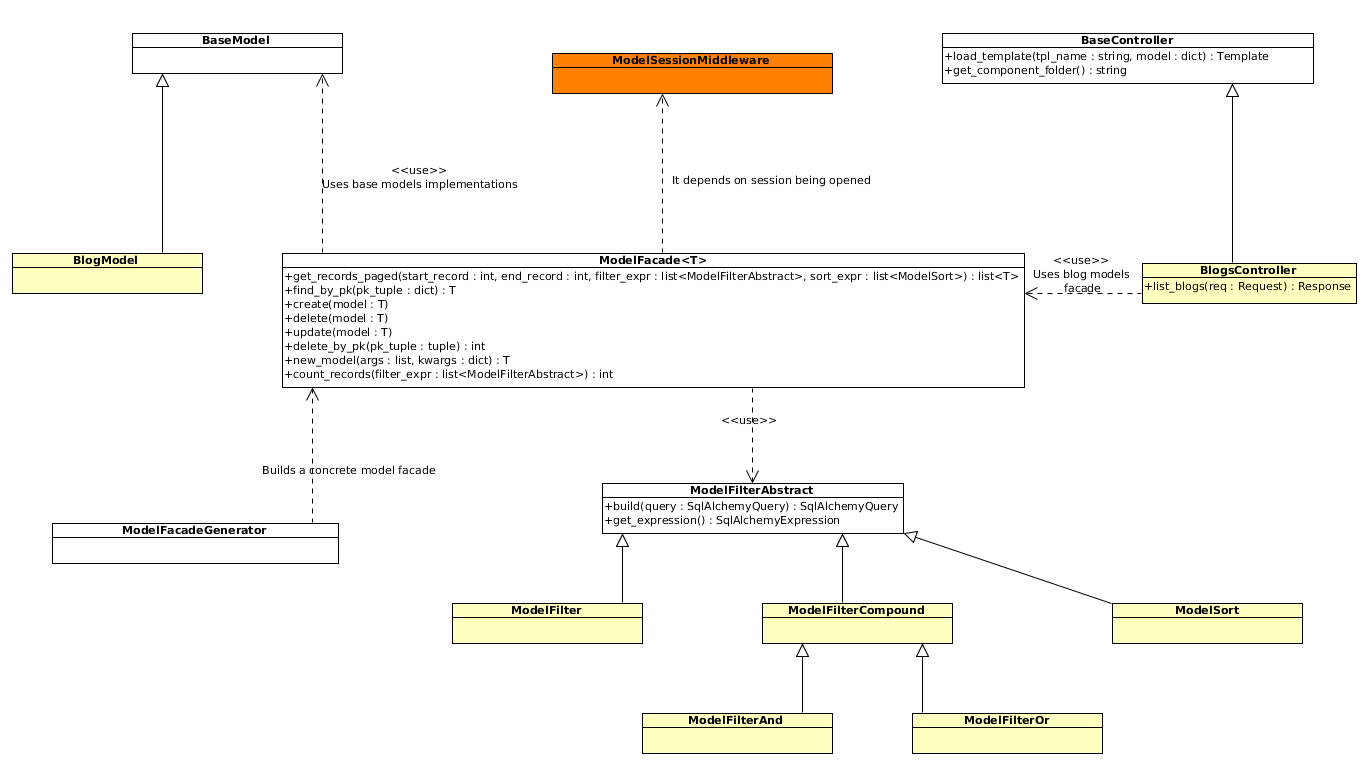
\includegraphics{mvc.png}
\index{fn\_handler (fantastico.mvc.controller\_decorators.Controller attribute)}

\begin{fulllineitems}
\phantomsection\label{features/mvc:fantastico.mvc.controller_decorators.Controller.fn_handler}\pysigline{\bfcode{fn\_handler}}
This property retrieves the method which is executed by this controller.

\end{fulllineitems}

\index{get\_registered\_routes() (fantastico.mvc.controller\_decorators.Controller class method)}

\begin{fulllineitems}
\phantomsection\label{features/mvc:fantastico.mvc.controller_decorators.Controller.get_registered_routes}\pysiglinewithargsret{\strong{classmethod }\bfcode{get\_registered\_routes}}{}{}
This class methods retrieve all registered routes through Controller decorator.

\end{fulllineitems}

\index{method (fantastico.mvc.controller\_decorators.Controller attribute)}

\begin{fulllineitems}
\phantomsection\label{features/mvc:fantastico.mvc.controller_decorators.Controller.method}\pysigline{\bfcode{method}}
This property retrieves the method(s) for which this controller can be invoked. Most of the time only one value is
retrieved.

\end{fulllineitems}

\index{models (fantastico.mvc.controller\_decorators.Controller attribute)}

\begin{fulllineitems}
\phantomsection\label{features/mvc:fantastico.mvc.controller_decorators.Controller.models}\pysigline{\bfcode{models}}
This property retrieves all the models required by this controller in order to work correctly.

\end{fulllineitems}

\index{url (fantastico.mvc.controller\_decorators.Controller attribute)}

\begin{fulllineitems}
\phantomsection\label{features/mvc:fantastico.mvc.controller_decorators.Controller.url}\pysigline{\bfcode{url}}
This property retrieves the url used when registering this controller.

\end{fulllineitems}


\end{fulllineitems}


If you want to find more details and use cases for controller read {\hyperref[features/mvc:core-controller-section]{\emph{Controller}}} section.


\subsection{Model}
\label{features/mvc:model}
A model is a very simple object that inherits \code{fantastico.mvc.models.BaseModel}.

In order for models to work correctly and to be injected correctly into controller you must make sure you have
a valid database configuration in your settings file. By default, {\hyperref[get_started/settings:fantastico.settings.BasicSettings]{\code{fantastico.settings.BasicSettings}}} provides a usable
database configuration.

\begin{Verbatim}[commandchars=\\\{\}]
\PYG{c}{\PYGZsh{} fantastico.settings.BasicSettings}
\PYG{n+nd}{@property}
\PYG{k}{def} \PYG{n+nf}{database\PYGZus{}config}\PYG{p}{(}\PYG{n+nb+bp}{self}\PYG{p}{)}\PYG{p}{:}
    \PYG{k}{return} \PYG{p}{\PYGZob{}}\PYG{l+s}{\PYGZdq{}}\PYG{l+s}{drivername}\PYG{l+s}{\PYGZdq{}}\PYG{p}{:} \PYG{l+s}{\PYGZdq{}}\PYG{l+s}{mysql+mysqldb}\PYG{l+s}{\PYGZdq{}}\PYG{p}{,}
            \PYG{l+s}{\PYGZdq{}}\PYG{l+s}{username}\PYG{l+s}{\PYGZdq{}}\PYG{p}{:} \PYG{l+s}{\PYGZdq{}}\PYG{l+s}{fantastico}\PYG{l+s}{\PYGZdq{}}\PYG{p}{,}
            \PYG{l+s}{\PYGZdq{}}\PYG{l+s}{password}\PYG{l+s}{\PYGZdq{}}\PYG{p}{:} \PYG{l+s}{\PYGZdq{}}\PYG{l+s}{12345}\PYG{l+s}{\PYGZdq{}}\PYG{p}{,}
            \PYG{l+s}{\PYGZdq{}}\PYG{l+s}{host}\PYG{l+s}{\PYGZdq{}}\PYG{p}{:} \PYG{l+s}{\PYGZdq{}}\PYG{l+s}{localhost}\PYG{l+s}{\PYGZdq{}}\PYG{p}{,}
            \PYG{l+s}{\PYGZdq{}}\PYG{l+s}{port}\PYG{l+s}{\PYGZdq{}}\PYG{p}{:} \PYG{l+m+mi}{3306}\PYG{p}{,}
            \PYG{l+s}{\PYGZdq{}}\PYG{l+s}{database}\PYG{l+s}{\PYGZdq{}}\PYG{p}{:} \PYG{l+s}{\PYGZdq{}}\PYG{l+s}{fantastico}\PYG{l+s}{\PYGZdq{}}\PYG{p}{,}
            \PYG{l+s}{\PYGZdq{}}\PYG{l+s}{show\PYGZus{}sql}\PYG{l+s}{\PYGZdq{}}\PYG{p}{:} \PYG{n+nb+bp}{True}\PYG{p}{\PYGZcb{}}
\end{Verbatim}

By default, each time a new build is generated for fantastico each environment is validated to ensure connectivity to configured
database works.

There are multiple ways in how a model is used but the easiest way is to use an autogenerated model facade:
\index{ModelFacade (class in fantastico.mvc.model\_facade)}

\begin{fulllineitems}
\phantomsection\label{features/mvc:fantastico.mvc.model_facade.ModelFacade}\pysiglinewithargsret{\strong{class }\code{fantastico.mvc.model\_facade.}\bfcode{ModelFacade}}{\emph{model\_cls}, \emph{session}}{}
This class provides a generic model facade factory. In order to work \textbf{Fantastico} base model it is recommended
to use autogenerated facade objects. A facade object is binded to a given model and given database session.
\index{count\_records() (fantastico.mvc.model\_facade.ModelFacade method)}

\begin{fulllineitems}
\phantomsection\label{features/mvc:fantastico.mvc.model_facade.ModelFacade.count_records}\pysiglinewithargsret{\bfcode{count\_records}}{\emph{filter\_expr=None}}{}
This method is used for counting the number of records from underlining facade. In addition it applies the
filter expressions specified (if any).

\begin{Verbatim}[commandchars=\\\{\}]
\PYG{n}{records} \PYG{o}{=} \PYG{n}{facade}\PYG{o}{.}\PYG{n}{count\PYGZus{}records}\PYG{p}{(}
                           \PYG{n}{filter\PYGZus{}expr}\PYG{o}{=}\PYG{n}{ModelFilterAnd}\PYG{p}{(}
                                           \PYG{n}{ModelFilter}\PYG{p}{(}\PYG{n}{Blog}\PYG{o}{.}\PYG{n}{id}\PYG{p}{,} \PYG{l+m+mi}{1}\PYG{p}{,} \PYG{n}{ModelFilter}\PYG{o}{.}\PYG{n}{GT}\PYG{p}{)}\PYG{p}{,}
                                           \PYG{n}{ModelFilter}\PYG{p}{(}\PYG{n}{Blog}\PYG{o}{.}\PYG{n}{id}\PYG{p}{,} \PYG{l+m+mi}{5}\PYG{p}{,} \PYG{n}{ModelFilter}\PYG{o}{.}\PYG{n}{LT}\PYG{p}{)}\PYG{p}{)}\PYG{p}{)}
\end{Verbatim}
\begin{quote}\begin{description}
\item[{Parameters}] \leavevmode
\textbf{filter\_expr} (\emph{list}) -- A list of {\hyperref[features/mvc:fantastico.mvc.models.model_filter.ModelFilterAbstract]{\code{fantastico.mvc.models.model\_filter.ModelFilterAbstract}}} which are applied in order.

\item[{Raises {\hyperref[features/exceptions:fantastico.exceptions.FantasticoDbError]{fantastico.exceptions.FantasticoDbError}}}] \leavevmode
This exception is raised whenever an exception occurs in retrieving
desired dataset. The underlining session used is automatically rollbacked in order to guarantee data integrity.

\end{description}\end{quote}

\end{fulllineitems}

\index{create() (fantastico.mvc.model\_facade.ModelFacade method)}

\begin{fulllineitems}
\phantomsection\label{features/mvc:fantastico.mvc.model_facade.ModelFacade.create}\pysiglinewithargsret{\bfcode{create}}{\emph{model}}{}
This method add the given model in the database.

\begin{Verbatim}[commandchars=\\\{\}]
\PYG{k}{class} \PYG{n+nc}{PersonModel}\PYG{p}{(}\PYG{n}{BASEMODEL}\PYG{p}{)}\PYG{p}{:}
    \PYG{n}{\PYGZus{}\PYGZus{}tablename\PYGZus{}\PYGZus{}} \PYG{o}{=} \PYG{l+s}{\PYGZdq{}}\PYG{l+s}{persons}\PYG{l+s}{\PYGZdq{}}

    \PYG{n+nb}{id} \PYG{o}{=} \PYG{n}{Column}\PYG{p}{(}\PYG{l+s}{\PYGZdq{}}\PYG{l+s}{id}\PYG{l+s}{\PYGZdq{}}\PYG{p}{,} \PYG{n}{Integer}\PYG{p}{,} \PYG{n}{autoincrement}\PYG{o}{=}\PYG{n+nb+bp}{True}\PYG{p}{,} \PYG{n}{primary\PYGZus{}key}\PYG{o}{=}\PYG{n+nb+bp}{True}\PYG{p}{)}
    \PYG{n}{first\PYGZus{}name} \PYG{o}{=} \PYG{n}{Column}\PYG{p}{(}\PYG{l+s}{\PYGZdq{}}\PYG{l+s}{first\PYGZus{}name}\PYG{l+s}{\PYGZdq{}}\PYG{p}{,} \PYG{n}{String}\PYG{p}{(}\PYG{l+m+mi}{50}\PYG{p}{)}\PYG{p}{)}
    \PYG{n}{last\PYGZus{}name} \PYG{o}{=} \PYG{n}{Column}\PYG{p}{(}\PYG{l+s}{\PYGZdq{}}\PYG{l+s}{last\PYGZus{}name}\PYG{l+s}{\PYGZdq{}}\PYG{p}{,} \PYG{n}{String}\PYG{p}{(}\PYG{l+m+mi}{50}\PYG{p}{)}\PYG{p}{)}

    \PYG{k}{def} \PYG{n+nf}{\PYGZus{}\PYGZus{}init\PYGZus{}\PYGZus{}}\PYG{p}{(}\PYG{n+nb+bp}{self}\PYG{p}{,} \PYG{n}{first\PYGZus{}name}\PYG{p}{,} \PYG{n}{last\PYGZus{}name}\PYG{p}{)}\PYG{p}{:}
        \PYG{n+nb+bp}{self}\PYG{o}{.}\PYG{n}{first\PYGZus{}name} \PYG{o}{=} \PYG{n}{first\PYGZus{}name}
        \PYG{n+nb+bp}{self}\PYG{o}{.}\PYG{n}{last\PYGZus{}name} \PYG{o}{=} \PYG{n}{last\PYGZus{}name}

\PYG{n}{facade} \PYG{o}{=} \PYG{n}{ModelFacade}\PYG{p}{(}\PYG{n}{PersonModel}\PYG{p}{,} \PYG{n}{fantastico}\PYG{o}{.}\PYG{n}{mvc}\PYG{o}{.}\PYG{n}{SESSION}\PYG{p}{)}

\PYG{n}{model} \PYG{o}{=} \PYG{n}{facade}\PYG{o}{.}\PYG{n}{new\PYGZus{}model}\PYG{p}{(}\PYG{l+s}{\PYGZdq{}}\PYG{l+s}{John}\PYG{l+s}{\PYGZdq{}}\PYG{p}{,} \PYG{n}{last\PYGZus{}name}\PYG{o}{=}\PYG{l+s}{\PYGZdq{}}\PYG{l+s}{Doe}\PYG{l+s}{\PYGZdq{}}\PYG{p}{)}
\PYG{n}{facade}\PYG{o}{.}\PYG{n}{create}\PYG{p}{(}\PYG{n}{model}\PYG{p}{)}
\end{Verbatim}
\begin{quote}\begin{description}
\item[{Returns}] \leavevmode
The newly generated primary key or the specified primary key (it might be a scalar value or a tuple).

\item[{Raises {\hyperref[features/exceptions:fantastico.exceptions.FantasticoDbError]{fantastico.exceptions.FantasticoDbError}}}] \leavevmode
Raised when an unhandled exception occurs. By default, session
is rollback automatically so that other consumers can still work as expected.

\end{description}\end{quote}

\end{fulllineitems}

\index{delete() (fantastico.mvc.model\_facade.ModelFacade method)}

\begin{fulllineitems}
\phantomsection\label{features/mvc:fantastico.mvc.model_facade.ModelFacade.delete}\pysiglinewithargsret{\bfcode{delete}}{\emph{model}}{}
This method deletes a given model from database. Below you can find a simple example of how to use this:

\begin{Verbatim}[commandchars=\\\{\}]
\PYG{k}{class} \PYG{n+nc}{PersonModel}\PYG{p}{(}\PYG{n}{BASEMODEL}\PYG{p}{)}\PYG{p}{:}
    \PYG{n}{\PYGZus{}\PYGZus{}tablename\PYGZus{}\PYGZus{}} \PYG{o}{=} \PYG{l+s}{\PYGZdq{}}\PYG{l+s}{persons}\PYG{l+s}{\PYGZdq{}}

    \PYG{n+nb}{id} \PYG{o}{=} \PYG{n}{Column}\PYG{p}{(}\PYG{l+s}{\PYGZdq{}}\PYG{l+s}{id}\PYG{l+s}{\PYGZdq{}}\PYG{p}{,} \PYG{n}{Integer}\PYG{p}{,} \PYG{n}{autoincrement}\PYG{o}{=}\PYG{n+nb+bp}{True}\PYG{p}{,} \PYG{n}{primary\PYGZus{}key}\PYG{o}{=}\PYG{n+nb+bp}{True}\PYG{p}{)}
    \PYG{n}{first\PYGZus{}name} \PYG{o}{=} \PYG{n}{Column}\PYG{p}{(}\PYG{l+s}{\PYGZdq{}}\PYG{l+s}{first\PYGZus{}name}\PYG{l+s}{\PYGZdq{}}\PYG{p}{,} \PYG{n}{String}\PYG{p}{(}\PYG{l+m+mi}{50}\PYG{p}{)}\PYG{p}{)}
    \PYG{n}{last\PYGZus{}name} \PYG{o}{=} \PYG{n}{Column}\PYG{p}{(}\PYG{l+s}{\PYGZdq{}}\PYG{l+s}{last\PYGZus{}name}\PYG{l+s}{\PYGZdq{}}\PYG{p}{,} \PYG{n}{String}\PYG{p}{(}\PYG{l+m+mi}{50}\PYG{p}{)}\PYG{p}{)}

    \PYG{k}{def} \PYG{n+nf}{\PYGZus{}\PYGZus{}init\PYGZus{}\PYGZus{}}\PYG{p}{(}\PYG{n+nb+bp}{self}\PYG{p}{,} \PYG{n}{first\PYGZus{}name}\PYG{p}{,} \PYG{n}{last\PYGZus{}name}\PYG{p}{)}\PYG{p}{:}
        \PYG{n+nb+bp}{self}\PYG{o}{.}\PYG{n}{first\PYGZus{}name} \PYG{o}{=} \PYG{n}{first\PYGZus{}name}
        \PYG{n+nb+bp}{self}\PYG{o}{.}\PYG{n}{last\PYGZus{}name} \PYG{o}{=} \PYG{n}{last\PYGZus{}name}

\PYG{n}{facade} \PYG{o}{=} \PYG{n}{ModelFacade}\PYG{p}{(}\PYG{n}{PersonModel}\PYG{p}{,} \PYG{n}{fantastico}\PYG{o}{.}\PYG{n}{mvc}\PYG{o}{.}\PYG{n}{SESSION}\PYG{p}{)}
\PYG{n}{model} \PYG{o}{=} \PYG{n}{facade}\PYG{o}{.}\PYG{n}{find\PYGZus{}by\PYGZus{}pk}\PYG{p}{(}\PYG{p}{\PYGZob{}}\PYG{n}{PersonModel}\PYG{o}{.}\PYG{n}{id}\PYG{p}{:} \PYG{l+m+mi}{1}\PYG{p}{\PYGZcb{}}\PYG{p}{)}
\PYG{n}{facade}\PYG{o}{.}\PYG{n}{delete}\PYG{p}{(}\PYG{n}{model}\PYG{p}{)}
\end{Verbatim}
\begin{quote}\begin{description}
\item[{Raises {\hyperref[features/exceptions:fantastico.exceptions.FantasticoDbError]{fantastico.exceptions.FantasticoDbError}}}] \leavevmode
Raised when an unhandled exception occurs. By default, session
is rollback automatically so that other consumers can still work as expected.

\end{description}\end{quote}

\end{fulllineitems}

\index{find\_by\_pk() (fantastico.mvc.model\_facade.ModelFacade method)}

\begin{fulllineitems}
\phantomsection\label{features/mvc:fantastico.mvc.model_facade.ModelFacade.find_by_pk}\pysiglinewithargsret{\bfcode{find\_by\_pk}}{\emph{pk\_values}}{}
This method returns the entity which matches the given primary key values.

\begin{Verbatim}[commandchars=\\\{\}]
\PYG{k}{class} \PYG{n+nc}{PersonModel}\PYG{p}{(}\PYG{n}{BASEMODEL}\PYG{p}{)}\PYG{p}{:}
    \PYG{n}{\PYGZus{}\PYGZus{}tablename\PYGZus{}\PYGZus{}} \PYG{o}{=} \PYG{l+s}{\PYGZdq{}}\PYG{l+s}{persons}\PYG{l+s}{\PYGZdq{}}

    \PYG{n+nb}{id} \PYG{o}{=} \PYG{n}{Column}\PYG{p}{(}\PYG{l+s}{\PYGZdq{}}\PYG{l+s}{id}\PYG{l+s}{\PYGZdq{}}\PYG{p}{,} \PYG{n}{Integer}\PYG{p}{,} \PYG{n}{autoincrement}\PYG{o}{=}\PYG{n+nb+bp}{True}\PYG{p}{,} \PYG{n}{primary\PYGZus{}key}\PYG{o}{=}\PYG{n+nb+bp}{True}\PYG{p}{)}
    \PYG{n}{first\PYGZus{}name} \PYG{o}{=} \PYG{n}{Column}\PYG{p}{(}\PYG{l+s}{\PYGZdq{}}\PYG{l+s}{first\PYGZus{}name}\PYG{l+s}{\PYGZdq{}}\PYG{p}{,} \PYG{n}{String}\PYG{p}{(}\PYG{l+m+mi}{50}\PYG{p}{)}\PYG{p}{)}
    \PYG{n}{last\PYGZus{}name} \PYG{o}{=} \PYG{n}{Column}\PYG{p}{(}\PYG{l+s}{\PYGZdq{}}\PYG{l+s}{last\PYGZus{}name}\PYG{l+s}{\PYGZdq{}}\PYG{p}{,} \PYG{n}{String}\PYG{p}{(}\PYG{l+m+mi}{50}\PYG{p}{)}\PYG{p}{)}

    \PYG{k}{def} \PYG{n+nf}{\PYGZus{}\PYGZus{}init\PYGZus{}\PYGZus{}}\PYG{p}{(}\PYG{n+nb+bp}{self}\PYG{p}{,} \PYG{n}{first\PYGZus{}name}\PYG{p}{,} \PYG{n}{last\PYGZus{}name}\PYG{p}{)}\PYG{p}{:}
        \PYG{n+nb+bp}{self}\PYG{o}{.}\PYG{n}{first\PYGZus{}name} \PYG{o}{=} \PYG{n}{first\PYGZus{}name}
        \PYG{n+nb+bp}{self}\PYG{o}{.}\PYG{n}{last\PYGZus{}name} \PYG{o}{=} \PYG{n}{last\PYGZus{}name}

\PYG{n}{facade} \PYG{o}{=} \PYG{n}{ModelFacade}\PYG{p}{(}\PYG{n}{PersonModel}\PYG{p}{,} \PYG{n}{fantastico}\PYG{o}{.}\PYG{n}{mvc}\PYG{o}{.}\PYG{n}{SESSION}\PYG{p}{)}
\PYG{n}{model} \PYG{o}{=} \PYG{n}{facade}\PYG{o}{.}\PYG{n}{find\PYGZus{}by\PYGZus{}pk}\PYG{p}{(}\PYG{p}{\PYGZob{}}\PYG{n}{PersonModel}\PYG{o}{.}\PYG{n}{id}\PYG{p}{:} \PYG{l+m+mi}{1}\PYG{p}{\PYGZcb{}}\PYG{p}{)}
\end{Verbatim}

\end{fulllineitems}

\index{get\_records\_paged() (fantastico.mvc.model\_facade.ModelFacade method)}

\begin{fulllineitems}
\phantomsection\label{features/mvc:fantastico.mvc.model_facade.ModelFacade.get_records_paged}\pysiglinewithargsret{\bfcode{get\_records\_paged}}{\emph{start\_record}, \emph{end\_record}, \emph{filter\_expr=None}, \emph{sort\_expr=None}}{}
This method retrieves all records matching the given filters sorted by the given expression.

\begin{Verbatim}[commandchars=\\\{\}]
\PYG{n}{records} \PYG{o}{=} \PYG{n}{facade}\PYG{o}{.}\PYG{n}{get\PYGZus{}records\PYGZus{}paged}\PYG{p}{(}\PYG{n}{start\PYGZus{}record}\PYG{o}{=}\PYG{l+m+mi}{0}\PYG{p}{,} \PYG{n}{end\PYGZus{}record}\PYG{o}{=}\PYG{l+m+mi}{5}\PYG{p}{,}
                           \PYG{n}{sort\PYGZus{}expr}\PYG{o}{=}\PYG{p}{[}\PYG{n}{ModelSort}\PYG{p}{(}\PYG{n}{Blog}\PYG{o}{.}\PYG{n}{create\PYGZus{}date}\PYG{p}{,} \PYG{n}{ModelSort}\PYG{o}{.}\PYG{n}{ASC}\PYG{p}{,}
                                      \PYG{n}{ModelSort}\PYG{p}{(}\PYG{n}{Blog}\PYG{o}{.}\PYG{n}{title}\PYG{p}{,} \PYG{n}{ModelSort}\PYG{o}{.}\PYG{n}{DESC}\PYG{p}{)}\PYG{p}{]}\PYG{p}{,}
                           \PYG{n}{filter\PYGZus{}expr}\PYG{o}{=}\PYG{n}{ModelFilterAnd}\PYG{p}{(}
                                           \PYG{n}{ModelFilter}\PYG{p}{(}\PYG{n}{Blog}\PYG{o}{.}\PYG{n}{id}\PYG{p}{,} \PYG{l+m+mi}{1}\PYG{p}{,} \PYG{n}{ModelFilter}\PYG{o}{.}\PYG{n}{GT}\PYG{p}{)}\PYG{p}{,}
                                           \PYG{n}{ModelFilter}\PYG{p}{(}\PYG{n}{Blog}\PYG{o}{.}\PYG{n}{id}\PYG{p}{,} \PYG{l+m+mi}{5}\PYG{p}{,} \PYG{n}{ModelFilter}\PYG{o}{.}\PYG{n}{LT}\PYG{p}{)}\PYG{p}{)}\PYG{p}{)}\PYG{p}{)}
\end{Verbatim}
\begin{quote}\begin{description}
\item[{Parameters}] \leavevmode\begin{itemize}
\item {} 
\textbf{start\_record} (\emph{int}) -- A zero indexed integer that specifies the first record number.

\item {} 
\textbf{end\_record} (\emph{int}) -- A zero indexed integer that specifies the last record number.

\item {} 
\textbf{filter\_expr} (\emph{list}) -- A list of {\hyperref[features/mvc:fantastico.mvc.models.model_filter.ModelFilterAbstract]{\code{fantastico.mvc.models.model\_filter.ModelFilterAbstract}}} which are applied in order.

\item {} 
\textbf{sort\_expr} (\emph{list}) -- A list of {\hyperref[features/mvc:fantastico.mvc.models.model_sort.ModelSort]{\code{fantastico.mvc.models.model\_sort.ModelSort}}} which are applied in order.

\end{itemize}

\item[{Returns}] \leavevmode
A list of matching records strongly converted to underlining model.

\item[{Raises {\hyperref[features/exceptions:fantastico.exceptions.FantasticoDbError]{fantastico.exceptions.FantasticoDbError}}}] \leavevmode
This exception is raised whenever an exception occurs in retrieving
desired dataset. The underlining session used is automatically rollbacked in order to guarantee data integrity.

\end{description}\end{quote}

\end{fulllineitems}

\index{model\_cls (fantastico.mvc.model\_facade.ModelFacade attribute)}

\begin{fulllineitems}
\phantomsection\label{features/mvc:fantastico.mvc.model_facade.ModelFacade.model_cls}\pysigline{\bfcode{model\_cls}}
This property holds the model based on which this facade is built.

\end{fulllineitems}

\index{model\_pk\_cols (fantastico.mvc.model\_facade.ModelFacade attribute)}

\begin{fulllineitems}
\phantomsection\label{features/mvc:fantastico.mvc.model_facade.ModelFacade.model_pk_cols}\pysigline{\bfcode{model\_pk\_cols}}
This property returns the model primary key columns as defined in the model cls.

\end{fulllineitems}

\index{new\_model() (fantastico.mvc.model\_facade.ModelFacade method)}

\begin{fulllineitems}
\phantomsection\label{features/mvc:fantastico.mvc.model_facade.ModelFacade.new_model}\pysiglinewithargsret{\bfcode{new\_model}}{\emph{*args}, \emph{**kwargs}}{}
This method is used to obtain an instance of the underlining model. Below you can find a very simple example:

\begin{Verbatim}[commandchars=\\\{\}]
\PYG{k}{class} \PYG{n+nc}{PersonModel}\PYG{p}{(}\PYG{n}{BASEMODEL}\PYG{p}{)}\PYG{p}{:}
    \PYG{n}{\PYGZus{}\PYGZus{}tablename\PYGZus{}\PYGZus{}} \PYG{o}{=} \PYG{l+s}{\PYGZdq{}}\PYG{l+s}{persons}\PYG{l+s}{\PYGZdq{}}

    \PYG{n+nb}{id} \PYG{o}{=} \PYG{n}{Column}\PYG{p}{(}\PYG{l+s}{\PYGZdq{}}\PYG{l+s}{id}\PYG{l+s}{\PYGZdq{}}\PYG{p}{,} \PYG{n}{Integer}\PYG{p}{,} \PYG{n}{autoincrement}\PYG{o}{=}\PYG{n+nb+bp}{True}\PYG{p}{,} \PYG{n}{primary\PYGZus{}key}\PYG{o}{=}\PYG{n+nb+bp}{True}\PYG{p}{)}
    \PYG{n}{first\PYGZus{}name} \PYG{o}{=} \PYG{n}{Column}\PYG{p}{(}\PYG{l+s}{\PYGZdq{}}\PYG{l+s}{first\PYGZus{}name}\PYG{l+s}{\PYGZdq{}}\PYG{p}{,} \PYG{n}{String}\PYG{p}{(}\PYG{l+m+mi}{50}\PYG{p}{)}\PYG{p}{)}
    \PYG{n}{last\PYGZus{}name} \PYG{o}{=} \PYG{n}{Column}\PYG{p}{(}\PYG{l+s}{\PYGZdq{}}\PYG{l+s}{last\PYGZus{}name}\PYG{l+s}{\PYGZdq{}}\PYG{p}{,} \PYG{n}{String}\PYG{p}{(}\PYG{l+m+mi}{50}\PYG{p}{)}\PYG{p}{)}

    \PYG{k}{def} \PYG{n+nf}{\PYGZus{}\PYGZus{}init\PYGZus{}\PYGZus{}}\PYG{p}{(}\PYG{n+nb+bp}{self}\PYG{p}{,} \PYG{n}{first\PYGZus{}name}\PYG{p}{,} \PYG{n}{last\PYGZus{}name}\PYG{p}{)}\PYG{p}{:}
        \PYG{n+nb+bp}{self}\PYG{o}{.}\PYG{n}{first\PYGZus{}name} \PYG{o}{=} \PYG{n}{first\PYGZus{}name}
        \PYG{n+nb+bp}{self}\PYG{o}{.}\PYG{n}{last\PYGZus{}name} \PYG{o}{=} \PYG{n}{last\PYGZus{}name}

\PYG{n}{facade} \PYG{o}{=} \PYG{n}{ModelFacade}\PYG{p}{(}\PYG{n}{PersonModel}\PYG{p}{,} \PYG{n}{fantastico}\PYG{o}{.}\PYG{n}{mvc}\PYG{o}{.}\PYG{n}{SESSION}\PYG{p}{)}

\PYG{n}{model} \PYG{o}{=} \PYG{n}{facade}\PYG{o}{.}\PYG{n}{new\PYGZus{}model}\PYG{p}{(}\PYG{l+s}{\PYGZdq{}}\PYG{l+s}{John}\PYG{l+s}{\PYGZdq{}}\PYG{p}{,} \PYG{n}{last\PYGZus{}name}\PYG{o}{=}\PYG{l+s}{\PYGZdq{}}\PYG{l+s}{Doe}\PYG{l+s}{\PYGZdq{}}\PYG{p}{)}
\end{Verbatim}
\begin{quote}\begin{description}
\item[{Parameters}] \leavevmode\begin{itemize}
\item {} 
\textbf{args} (\emph{list}) -- A list of positional arguments we want to pass to underlining model constructor.

\item {} 
\textbf{kwargs} (\emph{dict}) -- A dictionary containing named parameters we want to pass to underlining model constructor.

\end{itemize}

\item[{Returns}] \leavevmode
A BASEMODEL instance if everything is ok.

\end{description}\end{quote}

\end{fulllineitems}

\index{session (fantastico.mvc.model\_facade.ModelFacade attribute)}

\begin{fulllineitems}
\phantomsection\label{features/mvc:fantastico.mvc.model_facade.ModelFacade.session}\pysigline{\bfcode{session}}
This property returns the current sqlalchemy session used to access database.

\end{fulllineitems}

\index{update() (fantastico.mvc.model\_facade.ModelFacade method)}

\begin{fulllineitems}
\phantomsection\label{features/mvc:fantastico.mvc.model_facade.ModelFacade.update}\pysiglinewithargsret{\bfcode{update}}{\emph{model}}{}
This method updates an existing model from the database based on primary key.

\begin{Verbatim}[commandchars=\\\{\}]
\PYG{k}{class} \PYG{n+nc}{PersonModel}\PYG{p}{(}\PYG{n}{BASEMODEL}\PYG{p}{)}\PYG{p}{:}
    \PYG{n}{\PYGZus{}\PYGZus{}tablename\PYGZus{}\PYGZus{}} \PYG{o}{=} \PYG{l+s}{\PYGZdq{}}\PYG{l+s}{persons}\PYG{l+s}{\PYGZdq{}}

    \PYG{n+nb}{id} \PYG{o}{=} \PYG{n}{Column}\PYG{p}{(}\PYG{l+s}{\PYGZdq{}}\PYG{l+s}{id}\PYG{l+s}{\PYGZdq{}}\PYG{p}{,} \PYG{n}{Integer}\PYG{p}{,} \PYG{n}{autoincrement}\PYG{o}{=}\PYG{n+nb+bp}{True}\PYG{p}{,} \PYG{n}{primary\PYGZus{}key}\PYG{o}{=}\PYG{n+nb+bp}{True}\PYG{p}{)}
    \PYG{n}{first\PYGZus{}name} \PYG{o}{=} \PYG{n}{Column}\PYG{p}{(}\PYG{l+s}{\PYGZdq{}}\PYG{l+s}{first\PYGZus{}name}\PYG{l+s}{\PYGZdq{}}\PYG{p}{,} \PYG{n}{String}\PYG{p}{(}\PYG{l+m+mi}{50}\PYG{p}{)}\PYG{p}{)}
    \PYG{n}{last\PYGZus{}name} \PYG{o}{=} \PYG{n}{Column}\PYG{p}{(}\PYG{l+s}{\PYGZdq{}}\PYG{l+s}{last\PYGZus{}name}\PYG{l+s}{\PYGZdq{}}\PYG{p}{,} \PYG{n}{String}\PYG{p}{(}\PYG{l+m+mi}{50}\PYG{p}{)}\PYG{p}{)}

    \PYG{k}{def} \PYG{n+nf}{\PYGZus{}\PYGZus{}init\PYGZus{}\PYGZus{}}\PYG{p}{(}\PYG{n+nb+bp}{self}\PYG{p}{,} \PYG{n}{first\PYGZus{}name}\PYG{p}{,} \PYG{n}{last\PYGZus{}name}\PYG{p}{)}\PYG{p}{:}
        \PYG{n+nb+bp}{self}\PYG{o}{.}\PYG{n}{first\PYGZus{}name} \PYG{o}{=} \PYG{n}{first\PYGZus{}name}
        \PYG{n+nb+bp}{self}\PYG{o}{.}\PYG{n}{last\PYGZus{}name} \PYG{o}{=} \PYG{n}{last\PYGZus{}name}

\PYG{n}{facade} \PYG{o}{=} \PYG{n}{ModelFacade}\PYG{p}{(}\PYG{n}{PersonModel}\PYG{p}{,} \PYG{n}{fantastico}\PYG{o}{.}\PYG{n}{mvc}\PYG{o}{.}\PYG{n}{SESSION}\PYG{p}{)}

\PYG{n}{model} \PYG{o}{=} \PYG{n}{facade}\PYG{o}{.}\PYG{n}{new\PYGZus{}model}\PYG{p}{(}\PYG{l+s}{\PYGZdq{}}\PYG{l+s}{John}\PYG{l+s}{\PYGZdq{}}\PYG{p}{,} \PYG{n}{last\PYGZus{}name}\PYG{o}{=}\PYG{l+s}{\PYGZdq{}}\PYG{l+s}{Doe}\PYG{l+s}{\PYGZdq{}}\PYG{p}{)}
\PYG{n}{model}\PYG{o}{.}\PYG{n}{id} \PYG{o}{=} \PYG{l+m+mi}{5}
\PYG{n}{facade}\PYG{o}{.}\PYG{n}{update}\PYG{p}{(}\PYG{n}{model}\PYG{p}{)}
\end{Verbatim}
\begin{quote}\begin{description}
\item[{Raises}] \leavevmode\begin{itemize}
\item {} 
{\hyperref[features/exceptions:fantastico.exceptions.FantasticoDbNotFoundError]{\textbf{fantastico.exceptions.FantasticoDbNotFoundError}}} -- Raised when the given model does not exist in database.
By default, session is rollback automatically so that other consumers can still work as expected.

\item {} 
{\hyperref[features/exceptions:fantastico.exceptions.FantasticoDbError]{\textbf{fantastico.exceptions.FantasticoDbError}}} -- Raised when an unhandled exception occurs. By default, session
is rollback automatically so that other consumers can still work as expected.

\end{itemize}

\end{description}\end{quote}

\end{fulllineitems}


\end{fulllineitems}


If you are using the \textbf{Fantastico MVC} support you don't need to manually create a model facade instance because
{\hyperref[features/mvc:fantastico.mvc.controller_decorators.Controller]{\code{fantastico.mvc.controller\_decorators.Controller}}} injects defined models automatically.


\subsection{View}
\label{features/mvc:view}
A view can be a simple html plain file or html + jinja2 enriched support. You can read more about \textbf{Jinja2}
\href{http://jinja.pocoo.org/docs/}{here}. Usually, if you need some logical block statements in your view (if, for, ...)
it is easier to use jinja 2 template engine. The good news is that you can easily embed jinja 2 markup in your views
and it will be rendered automatically.


\subsection{Controller}
\label{features/mvc:controller}\label{features/mvc:core-controller-section}
A controller is the \emph{brain}; it actually combines a model execute some business logic and pass data to the desired view
that needs to be rendered. In some cases you don't really need view in order to provide the logic you want:
\begin{itemize}
\item {} 
A REST Web service.

\item {} 
A RSS feed provider.

\item {} 
A file download service

\end{itemize}

Though writing REST services does not require a view, you can load external text templates that might be useful for assembling the
response:
\begin{itemize}
\item {} 
An invoice generator service

\item {} 
An xml file that must be filled with product data

\item {} 
A \href{http://en.wikipedia.org/wiki/VCard}{vCard}. export service.

\end{itemize}

If you want to read a small tutorial and to start coding very fast on Fantastico MVC read {\hyperref[how_to/mvc_how_to::doc]{\emph{MVC How to}}}. Controller
API is documented \code{fantastico.mvc.controller\_decorator.Controller}.
\index{ControllerRouteLoader (class in fantastico.mvc.controller\_registrator)}

\begin{fulllineitems}
\phantomsection\label{features/mvc:fantastico.mvc.controller_registrator.ControllerRouteLoader}\pysiglinewithargsret{\strong{class }\code{fantastico.mvc.controller\_registrator.}\bfcode{ControllerRouteLoader}}{\emph{settings\_facade=\textless{}class `fantastico.settings.SettingsFacade'\textgreater{}}, \emph{scanned\_folder=None}, \emph{ignore\_prefix=None}}{}
This class provides a route loader that is capable of scanning the disk and registering only the routes that
contain a controller decorator in them. This happens when \textbf{Fantastico} servers starts. In standard configuration
it ignores tests subfolder as well as test\_* / itest\_* modules.
\index{load\_routes() (fantastico.mvc.controller\_registrator.ControllerRouteLoader method)}

\begin{fulllineitems}
\phantomsection\label{features/mvc:fantastico.mvc.controller_registrator.ControllerRouteLoader.load_routes}\pysiglinewithargsret{\bfcode{load\_routes}}{}{}
This method is used for loading all routes that are mapped through
{\hyperref[features/mvc:fantastico.mvc.controller_decorators.Controller]{\code{fantastico.mvc.controller\_decorators.Controller}}} decorator.

\end{fulllineitems}

\index{scanned\_folders (fantastico.mvc.controller\_registrator.ControllerRouteLoader attribute)}

\begin{fulllineitems}
\phantomsection\label{features/mvc:fantastico.mvc.controller_registrator.ControllerRouteLoader.scanned_folders}\pysigline{\bfcode{scanned\_folders}}
This property returns the currently scanned folder from where mvc routes are collected.

\end{fulllineitems}


\end{fulllineitems}

\index{BaseController (class in fantastico.mvc.base\_controller)}

\begin{fulllineitems}
\phantomsection\label{features/mvc:fantastico.mvc.base_controller.BaseController}\pysiglinewithargsret{\strong{class }\code{fantastico.mvc.base\_controller.}\bfcode{BaseController}}{\emph{settings\_facade}}{}
This class provides common methods useful for every concrete controller. Even if no type checking is done in
Fantastico it is recommended that every controller implementation inherits this class.
\index{curr\_request (fantastico.mvc.base\_controller.BaseController attribute)}

\begin{fulllineitems}
\phantomsection\label{features/mvc:fantastico.mvc.base_controller.BaseController.curr_request}\pysigline{\bfcode{curr\_request}}
This property returns the current http request being processed.

\end{fulllineitems}

\index{get\_component\_folder() (fantastico.mvc.base\_controller.BaseController method)}

\begin{fulllineitems}
\phantomsection\label{features/mvc:fantastico.mvc.base_controller.BaseController.get_component_folder}\pysiglinewithargsret{\bfcode{get\_component\_folder}}{}{}
This method is used to retrieve the component folder name under which this controller is defined.

\end{fulllineitems}

\index{load\_template() (fantastico.mvc.base\_controller.BaseController method)}

\begin{fulllineitems}
\phantomsection\label{features/mvc:fantastico.mvc.base_controller.BaseController.load_template}\pysiglinewithargsret{\bfcode{load\_template}}{\emph{tpl\_name}, \emph{model\_data=None}, \emph{get\_template=\textless{}function get\_template at 0x1516408\textgreater{}}, \emph{enable\_global\_folder=False}}{}
This method is responsible for loading a template from disk and render it using the given model data.

\begin{Verbatim}[commandchars=\\\{\}]
\PYG{n+nd}{@ControllerProvider}\PYG{p}{(}\PYG{p}{)}
\PYG{k}{class} \PYG{n+nc}{TestController}\PYG{p}{(}\PYG{n}{BaseController}\PYG{p}{)}\PYG{p}{:}
    \PYG{n+nd}{@Controller}\PYG{p}{(}\PYG{n}{url}\PYG{o}{=}\PYG{l+s}{\PYGZdq{}}\PYG{l+s}{/simple/test/hello}\PYG{l+s}{\PYGZdq{}}\PYG{p}{,} \PYG{n}{method}\PYG{o}{=}\PYG{l+s}{\PYGZdq{}}\PYG{l+s}{GET}\PYG{l+s}{\PYGZdq{}}\PYG{p}{)}
    \PYG{k}{def} \PYG{n+nf}{say\PYGZus{}hello}\PYG{p}{(}\PYG{n+nb+bp}{self}\PYG{p}{,} \PYG{n}{request}\PYG{p}{)}\PYG{p}{:}
        \PYG{k}{return} \PYG{n}{Response}\PYG{p}{(}\PYG{n+nb+bp}{self}\PYG{o}{.}\PYG{n}{load\PYGZus{}template}\PYG{p}{(}\PYG{l+s}{\PYGZdq{}}\PYG{l+s}{/hello.html}\PYG{l+s}{\PYGZdq{}}\PYG{p}{)}\PYG{p}{)}
\end{Verbatim}

The above snippet will search for \textbf{hello.html} into component folder/views/.

\end{fulllineitems}


\end{fulllineitems}



\subsubsection{Available filters}
\label{features/mvc:available-filters}\index{ModelFilterAbstract (class in fantastico.mvc.models.model\_filter)}

\begin{fulllineitems}
\phantomsection\label{features/mvc:fantastico.mvc.models.model_filter.ModelFilterAbstract}\pysigline{\strong{class }\code{fantastico.mvc.models.model\_filter.}\bfcode{ModelFilterAbstract}}
This is the base class that defines the contract a model filter must follow. A model filter is a class that decouples
sqlalchemy framework from Fantastico MVC. This is required because in the future we might want to change the ORM that
powers Fantastico without breaking all existing code.

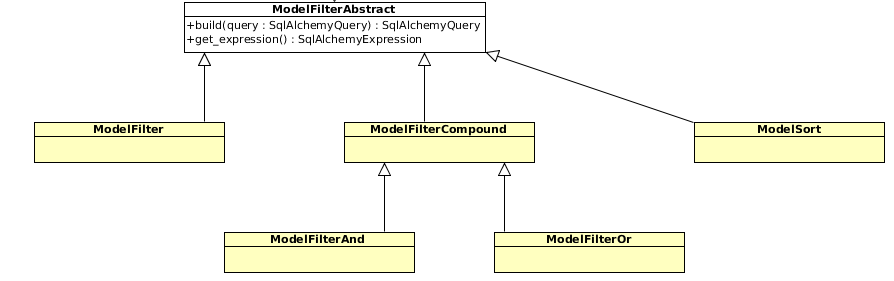
\includegraphics{mvc_filters.png}

For seeing how to implement filters (probably you won't need to do this) see some existing filters:
\begin{itemize}
\item {} 
{\hyperref[features/mvc:fantastico.mvc.models.model_filter.ModelFilter]{\code{fantastico.mvc.models.model\_filter.ModelFilter}}}

\item {} 
{\hyperref[features/mvc:fantastico.mvc.models.model_filter_compound.ModelFilterCompound]{\code{fantastico.mvc.models.model\_filter\_compound.ModelFilterCompound}}}

\item {} 
{\hyperref[features/mvc:fantastico.mvc.models.model_filter_compound.ModelFilterAnd]{\code{fantastico.mvc.models.model\_filter\_compound.ModelFilterAnd}}}

\item {} 
{\hyperref[features/mvc:fantastico.mvc.models.model_filter_compound.ModelFilterOr]{\code{fantastico.mvc.models.model\_filter\_compound.ModelFilterOr}}}

\end{itemize}
\index{build() (fantastico.mvc.models.model\_filter.ModelFilterAbstract method)}

\begin{fulllineitems}
\phantomsection\label{features/mvc:fantastico.mvc.models.model_filter.ModelFilterAbstract.build}\pysiglinewithargsret{\bfcode{build}}{\emph{query}}{}
This method is used for appending the current filter to the query using sqlalchemy specific language.

\end{fulllineitems}

\index{get\_expression() (fantastico.mvc.models.model\_filter.ModelFilterAbstract method)}

\begin{fulllineitems}
\phantomsection\label{features/mvc:fantastico.mvc.models.model_filter.ModelFilterAbstract.get_expression}\pysiglinewithargsret{\bfcode{get\_expression}}{}{}
This method is used for retrieving native sqlalchemy expression held by this filter.

\end{fulllineitems}


\end{fulllineitems}

\index{ModelFilterCompound (class in fantastico.mvc.models.model\_filter\_compound)}

\begin{fulllineitems}
\phantomsection\label{features/mvc:fantastico.mvc.models.model_filter_compound.ModelFilterCompound}\pysiglinewithargsret{\strong{class }\code{fantastico.mvc.models.model\_filter\_compound.}\bfcode{ModelFilterCompound}}{\emph{operation}, \emph{*args}}{}
This class provides the api for compounding ModelFilter objects into a specified sql alchemy operation.
\index{build() (fantastico.mvc.models.model\_filter\_compound.ModelFilterCompound method)}

\begin{fulllineitems}
\phantomsection\label{features/mvc:fantastico.mvc.models.model_filter_compound.ModelFilterCompound.build}\pysiglinewithargsret{\bfcode{build}}{\emph{query}}{}
This method transform the current compound statement into an sql alchemy filter.

\end{fulllineitems}

\index{get\_expression() (fantastico.mvc.models.model\_filter\_compound.ModelFilterCompound method)}

\begin{fulllineitems}
\phantomsection\label{features/mvc:fantastico.mvc.models.model_filter_compound.ModelFilterCompound.get_expression}\pysiglinewithargsret{\bfcode{get\_expression}}{}{}
This method transforms calculates sqlalchemy expression held by this filter.

\end{fulllineitems}

\index{model\_filters (fantastico.mvc.models.model\_filter\_compound.ModelFilterCompound attribute)}

\begin{fulllineitems}
\phantomsection\label{features/mvc:fantastico.mvc.models.model_filter_compound.ModelFilterCompound.model_filters}\pysigline{\bfcode{model\_filters}}
This property returns all ModelFilter instances being compound.

\end{fulllineitems}


\end{fulllineitems}

\index{ModelFilter (class in fantastico.mvc.models.model\_filter)}

\begin{fulllineitems}
\phantomsection\label{features/mvc:fantastico.mvc.models.model_filter.ModelFilter}\pysiglinewithargsret{\strong{class }\code{fantastico.mvc.models.model\_filter.}\bfcode{ModelFilter}}{\emph{column}, \emph{ref\_value}, \emph{operation}}{}
This class provides a model filter wrapper used to dynamically transform an operation to sql alchemy filter
statements. You can see below how to use it:

\begin{Verbatim}[commandchars=\\\{\}]
\PYG{n}{id\PYGZus{}gt\PYGZus{}filter} \PYG{o}{=} \PYG{n}{ModelFilter}\PYG{p}{(}\PYG{n}{PersonModel}\PYG{o}{.}\PYG{n}{id}\PYG{p}{,} \PYG{l+m+mi}{1}\PYG{p}{,} \PYG{n}{ModelFilter}\PYG{o}{.}\PYG{n}{GT}\PYG{p}{)}
\end{Verbatim}
\index{build() (fantastico.mvc.models.model\_filter.ModelFilter method)}

\begin{fulllineitems}
\phantomsection\label{features/mvc:fantastico.mvc.models.model_filter.ModelFilter.build}\pysiglinewithargsret{\bfcode{build}}{\emph{query}}{}
This method appends the current filter to a query object.

\end{fulllineitems}

\index{column (fantastico.mvc.models.model\_filter.ModelFilter attribute)}

\begin{fulllineitems}
\phantomsection\label{features/mvc:fantastico.mvc.models.model_filter.ModelFilter.column}\pysigline{\bfcode{column}}
This property holds the column used in the current filter.

\end{fulllineitems}

\index{get\_expression() (fantastico.mvc.models.model\_filter.ModelFilter method)}

\begin{fulllineitems}
\phantomsection\label{features/mvc:fantastico.mvc.models.model_filter.ModelFilter.get_expression}\pysiglinewithargsret{\bfcode{get\_expression}}{}{}
Method used to return the underlining sqlalchemy exception held by this filter.

\end{fulllineitems}

\index{get\_supported\_operations() (fantastico.mvc.models.model\_filter.ModelFilter static method)}

\begin{fulllineitems}
\phantomsection\label{features/mvc:fantastico.mvc.models.model_filter.ModelFilter.get_supported_operations}\pysiglinewithargsret{\strong{static }\bfcode{get\_supported\_operations}}{}{}
This method returns all supported operations for model filter. For now only the following operations are supported:
\begin{itemize}
\item {} 
GT - greater than comparison

\item {} 
GE - greater or equals than comparison

\item {} 
EQ - equals comparison

\item {} 
LE - less or equals than comparison

\item {} 
LT - less than comparison

\item {} 
LIKE - like comparison

\item {} 
IN - in comparison.

\end{itemize}

\end{fulllineitems}

\index{operation (fantastico.mvc.models.model\_filter.ModelFilter attribute)}

\begin{fulllineitems}
\phantomsection\label{features/mvc:fantastico.mvc.models.model_filter.ModelFilter.operation}\pysigline{\bfcode{operation}}
This property holds the operation used in the current filter.

\end{fulllineitems}

\index{ref\_value (fantastico.mvc.models.model\_filter.ModelFilter attribute)}

\begin{fulllineitems}
\phantomsection\label{features/mvc:fantastico.mvc.models.model_filter.ModelFilter.ref_value}\pysigline{\bfcode{ref\_value}}
This property holds the reference value used in the current filter.

\end{fulllineitems}


\end{fulllineitems}

\index{ModelFilterAnd (class in fantastico.mvc.models.model\_filter\_compound)}

\begin{fulllineitems}
\phantomsection\label{features/mvc:fantastico.mvc.models.model_filter_compound.ModelFilterAnd}\pysiglinewithargsret{\strong{class }\code{fantastico.mvc.models.model\_filter\_compound.}\bfcode{ModelFilterAnd}}{\emph{*args}}{}
This class provides a compound filter that allows \textbf{and} conditions against models. Below you can find a simple example:

\begin{Verbatim}[commandchars=\\\{\}]
\PYG{n}{id\PYGZus{}gt\PYGZus{}filter} \PYG{o}{=} \PYG{n}{ModelFilter}\PYG{p}{(}\PYG{n}{PersonModel}\PYG{o}{.}\PYG{n}{id}\PYG{p}{,} \PYG{l+m+mi}{1}\PYG{p}{,} \PYG{n}{ModelFilter}\PYG{o}{.}\PYG{n}{GT}\PYG{p}{)}
\PYG{n}{id\PYGZus{}lt\PYGZus{}filter} \PYG{o}{=} \PYG{n}{ModelFilter}\PYG{p}{(}\PYG{n}{PersonModel}\PYG{o}{.}\PYG{n}{id}\PYG{p}{,} \PYG{l+m+mi}{5}\PYG{p}{,} \PYG{n}{ModelFilter}\PYG{o}{.}\PYG{n}{LT}\PYG{p}{)}
\PYG{n}{name\PYGZus{}like\PYGZus{}filter} \PYG{o}{=} \PYG{n}{ModelFilter}\PYG{p}{(}\PYG{n}{PersonModel}\PYG{o}{.}\PYG{n}{name}\PYG{p}{,} \PYG{l+s}{\PYGZsq{}}\PYG{l+s+si}{\PYGZpc{}\PYGZpc{}}\PYG{l+s}{john}\PYG{l+s+si}{\PYGZpc{}\PYGZpc{}}\PYG{l+s}{\PYGZsq{}}\PYG{p}{,} \PYG{n}{ModelFilter}\PYG{o}{.}\PYG{n}{LIKE}\PYG{p}{)}

\PYG{n}{complex\PYGZus{}condition} \PYG{o}{=} \PYG{n}{ModelFilterAnd}\PYG{p}{(}\PYG{n}{id\PYGZus{}gt\PYGZus{}filter}\PYG{p}{,} \PYG{n}{id\PYGZus{}lt\PYGZus{}filter}\PYG{p}{,} \PYG{n}{name\PYGZus{}like\PYGZus{}filter}\PYG{p}{)}
\end{Verbatim}

\end{fulllineitems}

\index{ModelFilterOr (class in fantastico.mvc.models.model\_filter\_compound)}

\begin{fulllineitems}
\phantomsection\label{features/mvc:fantastico.mvc.models.model_filter_compound.ModelFilterOr}\pysiglinewithargsret{\strong{class }\code{fantastico.mvc.models.model\_filter\_compound.}\bfcode{ModelFilterOr}}{\emph{*args}}{}
This class provides a compound filter that allows \textbf{or} conditions against models. Below you can find a simple example:

\begin{Verbatim}[commandchars=\\\{\}]
\PYG{n}{id\PYGZus{}gt\PYGZus{}filter} \PYG{o}{=} \PYG{n}{ModelFilter}\PYG{p}{(}\PYG{n}{PersonModel}\PYG{o}{.}\PYG{n}{id}\PYG{p}{,} \PYG{l+m+mi}{1}\PYG{p}{,} \PYG{n}{ModelFilter}\PYG{o}{.}\PYG{n}{GT}\PYG{p}{)}
\PYG{n}{id\PYGZus{}lt\PYGZus{}filter} \PYG{o}{=} \PYG{n}{ModelFilter}\PYG{p}{(}\PYG{n}{PersonModel}\PYG{o}{.}\PYG{n}{id}\PYG{p}{,} \PYG{l+m+mi}{5}\PYG{p}{,} \PYG{n}{ModelFilter}\PYG{o}{.}\PYG{n}{LT}\PYG{p}{)}
\PYG{n}{name\PYGZus{}like\PYGZus{}filter} \PYG{o}{=} \PYG{n}{ModelFilter}\PYG{p}{(}\PYG{n}{PersonModel}\PYG{o}{.}\PYG{n}{name}\PYG{p}{,} \PYG{l+s}{\PYGZsq{}}\PYG{l+s+si}{\PYGZpc{}\PYGZpc{}}\PYG{l+s}{john}\PYG{l+s+si}{\PYGZpc{}\PYGZpc{}}\PYG{l+s}{\PYGZsq{}}\PYG{p}{,} \PYG{n}{ModelFilter}\PYG{o}{.}\PYG{n}{LIKE}\PYG{p}{)}

\PYG{n}{complex\PYGZus{}condition} \PYG{o}{=} \PYG{n}{ModelFilterOr}\PYG{p}{(}\PYG{n}{id\PYGZus{}gt\PYGZus{}filter}\PYG{p}{,} \PYG{n}{id\PYGZus{}lt\PYGZus{}filter}\PYG{p}{,} \PYG{n}{name\PYGZus{}like\PYGZus{}filter}\PYG{p}{)}
\end{Verbatim}

\end{fulllineitems}

\index{ModelSort (class in fantastico.mvc.models.model\_sort)}

\begin{fulllineitems}
\phantomsection\label{features/mvc:fantastico.mvc.models.model_sort.ModelSort}\pysiglinewithargsret{\strong{class }\code{fantastico.mvc.models.model\_sort.}\bfcode{ModelSort}}{\emph{column}, \emph{sort\_dir=None}}{}
This class provides a filter that knows how to sort rows from a query result set. It is extremely easy to use:

\begin{Verbatim}[commandchars=\\\{\}]
\PYG{n}{id\PYGZus{}sort\PYGZus{}asc} \PYG{o}{=} \PYG{n}{ModelSort}\PYG{p}{(}\PYG{n}{PersonModel}\PYG{o}{.}\PYG{n}{id}\PYG{p}{,} \PYG{n}{ModelSort}\PYG{o}{.}\PYG{n}{ASC}\PYG{p}{)}
\end{Verbatim}
\index{build() (fantastico.mvc.models.model\_sort.ModelSort method)}

\begin{fulllineitems}
\phantomsection\label{features/mvc:fantastico.mvc.models.model_sort.ModelSort.build}\pysiglinewithargsret{\bfcode{build}}{\emph{query}}{}
This method appends sort\_by clause to the given query.

\end{fulllineitems}

\index{column (fantastico.mvc.models.model\_sort.ModelSort attribute)}

\begin{fulllineitems}
\phantomsection\label{features/mvc:fantastico.mvc.models.model_sort.ModelSort.column}\pysigline{\bfcode{column}}
This property holds the column we are currently sorting.

\end{fulllineitems}

\index{get\_expression() (fantastico.mvc.models.model\_sort.ModelSort method)}

\begin{fulllineitems}
\phantomsection\label{features/mvc:fantastico.mvc.models.model_sort.ModelSort.get_expression}\pysiglinewithargsret{\bfcode{get\_expression}}{}{}
This method returns the sqlalchemy expression held by this filter.

\end{fulllineitems}

\index{get\_supported\_sort\_dirs() (fantastico.mvc.models.model\_sort.ModelSort method)}

\begin{fulllineitems}
\phantomsection\label{features/mvc:fantastico.mvc.models.model_sort.ModelSort.get_supported_sort_dirs}\pysiglinewithargsret{\bfcode{get\_supported\_sort\_dirs}}{}{}
This method returns all supported sort directions. Currently only ASC / DESC directions are supported.

\end{fulllineitems}

\index{sort\_dir (fantastico.mvc.models.model\_sort.ModelSort attribute)}

\begin{fulllineitems}
\phantomsection\label{features/mvc:fantastico.mvc.models.model_sort.ModelSort.sort_dir}\pysigline{\bfcode{sort\_dir}}
This property holds the sort direction we are currently using.

\end{fulllineitems}


\end{fulllineitems}



\subsection{Database session management}
\label{features/mvc:database-session-management}
We all know database session management is painful and adds a lot of boiler plate code. In fantastico you don't need
to manage database session by yourself. There is a dedicated middleware which automatically ensures there is an
active session ready to be used:
\index{ModelSessionMiddleware (class in fantastico.middleware.model\_session\_middleware)}

\begin{fulllineitems}
\phantomsection\label{features/mvc:fantastico.middleware.model_session_middleware.ModelSessionMiddleware}\pysiglinewithargsret{\strong{class }\code{fantastico.middleware.model\_session\_middleware.}\bfcode{ModelSessionMiddleware}}{\emph{app}, \emph{settings\_facade=\textless{}class `fantastico.settings.SettingsFacade'\textgreater{}}}{}
This class is responsible for managing database connections across requests. It also takes care of
connection data pools. By default, the middleware is automatically configured to open a connection. If
you don't need mvc (really improbable but still) you simply need to change your project active settings
profile. You can read more on {\hyperref[get_started/settings:fantastico.settings.BasicSettings]{\code{fantastico.settings.BasicSettings}}}

\end{fulllineitems}



\section{CORS}
\label{features/cors::doc}\label{features/cors:cors}
In Fantastico framework, CORS (cross origin resource sharing) can be enabled easily per each individual controller method.
\index{CorsEnabled (class in fantastico.mvc.controller\_decorators)}

\begin{fulllineitems}
\phantomsection\label{features/cors:fantastico.mvc.controller_decorators.CorsEnabled}\pysigline{\strong{class }\code{fantastico.mvc.controller\_decorators.}\bfcode{CorsEnabled}}
This class provides the cors behavior which ensures all cors required headers are appended to response. It is designed
to be used on controller methods decorated with @Controller attribute.

\begin{Verbatim}[commandchars=\\\{\}]
\PYG{n+nd}{@Controller}\PYG{p}{(}\PYG{n}{url}\PYG{o}{=}\PYG{l+s}{\PYGZdq{}}\PYG{l+s}{/api/filesystem/(?P\PYGZlt{}filename\PYGZgt{}.*)\PYGZdl{}}\PYG{l+s}{\PYGZdq{}}\PYG{p}{,} \PYG{n}{method}\PYG{o}{=}\PYG{l+s}{\PYGZdq{}}\PYG{l+s}{OPTIONS}\PYG{l+s}{\PYGZdq{}}\PYG{p}{)}
\PYG{n+nd}{@CorsEnabled}\PYG{p}{(}\PYG{p}{)}
\PYG{k}{def} \PYG{n+nf}{upload\PYGZus{}file\PYGZus{}options}\PYG{p}{(}\PYG{n+nb+bp}{self}\PYG{p}{,} \PYG{n}{request}\PYG{p}{,} \PYG{n}{filename}\PYG{p}{)}\PYG{p}{:}        
    \PYG{k}{pass}
\end{Verbatim}

As you can see there is no need to implement cors controller methods because the decorator does all the job.

\end{fulllineitems}


In addition to \textbf{CorsEnabled} decorator, you can also configure the framework to globally append some headers to each
response:
\begin{enumerate}
\item {} 
Go to your settins profile (see {\hyperref[get_started/settings:fantastico.settings.BasicSettings]{\code{fantastico.settings.BasicSettings}}})

\item {} 
Change \textbf{global\_response\_headers} property and add all desired headers (e.g: Access-Control-Allow-Origin: ``*'')

\end{enumerate}


\section{ROA (Resource Oriented Architecture)}
\label{features/roa:roa-resource-oriented-architecture}\label{features/roa::doc}
Resource Oriented Architecture (REST) is incredible popular nowadays for the following reasons:
\begin{itemize}
\item {} 
Increased scalability of applications.

\item {} 
Easy integration of systems.

\item {} 
Intuitive modelling of business problems.

\item {} 
Stateful imperative programming pains removed.

\end{itemize}

You can find many information about advantages of REST and why it is recommended to use such an architecure. For further reading
you can visit \href{http://en.wikipedia.org/wiki/Representational\_state\_transfer}{http://en.wikipedia.org/wiki/Representational\_state\_transfer}.

In Fantastisco framework we firmly encourage REST approach into projects. We even go a step further in this direction, by
standardising REST APIs and providing REST APIs generator over implemented models.


\subsection{Examples}
\label{features/roa:examples}

\subsection{Application settings stored in database}
\label{features/roa:application-settings-stored-in-database}
Imagine you have a model called \textbf{AppSetting} meant to define custom settings attributes which influence your application.

\begin{Verbatim}[commandchars=\\\{\}]
\PYG{k}{class} \PYG{n+nc}{AppSetting}\PYG{p}{(}\PYG{n}{BASEMODEL}\PYG{p}{)}\PYG{p}{:}
    \PYG{n}{\PYGZus{}\PYGZus{}tablename\PYGZus{}\PYGZus{}} \PYG{o}{=} \PYG{l+s}{\PYGZdq{}}\PYG{l+s}{app\PYGZus{}settings}\PYG{l+s}{\PYGZdq{}}

    \PYG{n+nb}{id} \PYG{o}{=} \PYG{n}{Column}\PYG{p}{(}\PYG{l+s}{\PYGZdq{}}\PYG{l+s}{id}\PYG{l+s}{\PYGZdq{}}\PYG{p}{,} \PYG{n}{Integer}\PYG{p}{,} \PYG{n}{primary\PYGZus{}key}\PYG{o}{=}\PYG{n+nb+bp}{True}\PYG{p}{,} \PYG{n}{autoincrement}\PYG{o}{=}\PYG{n+nb+bp}{True}\PYG{p}{)}
    \PYG{n}{name} \PYG{o}{=} \PYG{n}{Column}\PYG{p}{(}\PYG{l+s}{\PYGZdq{}}\PYG{l+s}{name}\PYG{l+s}{\PYGZdq{}}\PYG{p}{,} \PYG{n}{String}\PYG{p}{(}\PYG{l+m+mi}{50}\PYG{p}{)}\PYG{p}{,} \PYG{n}{unique}\PYG{o}{=}\PYG{n+nb+bp}{True}\PYG{p}{,} \PYG{n}{nullable}\PYG{o}{=}\PYG{n+nb+bp}{False}\PYG{p}{)}
    \PYG{n}{value} \PYG{o}{=} \PYG{n}{Column}\PYG{p}{(}\PYG{l+s}{\PYGZdq{}}\PYG{l+s}{value}\PYG{l+s}{\PYGZdq{}}\PYG{p}{,} \PYG{n}{Text}\PYG{p}{,} \PYG{n}{nullable}\PYG{o}{=}\PYG{n+nb+bp}{False}\PYG{p}{)}

    \PYG{k}{def} \PYG{n+nf}{\PYGZus{}\PYGZus{}init\PYGZus{}\PYGZus{}}\PYG{p}{(}\PYG{n+nb+bp}{self}\PYG{p}{,} \PYG{n}{name}\PYG{p}{,} \PYG{n}{value}\PYG{p}{)}\PYG{p}{:}
        \PYG{n+nb+bp}{self}\PYG{o}{.}\PYG{n}{name} \PYG{o}{=} \PYG{n}{name}
        \PYG{n+nb+bp}{self}\PYG{o}{.}\PYG{n}{value} \PYG{o}{=} \PYG{n}{value}
\end{Verbatim}

In a standard \textbf{MVC} ({\hyperref[features/mvc::doc]{\emph{Model View Controller}}}) web application once you have defined the above mentioned fantastico model you would
have to do the following: (for providing minimal CRUD)
\begin{enumerate}
\item {} 
Create a {\hyperref[features/mvc:fantastico.mvc.controller_decorators.Controller]{\code{fantastico.mvc.controller\_decorators.Controller}}}

\item {} 
Implement listing of custom settings
\begin{enumerate}
\item {} 
Support pagination.

\item {} 
Support filtering.

\item {} 
Support ordering.

\end{enumerate}

\item {} 
Implement individual custom setting retrieval (by id).

\item {} 
Implement Create custom setting.

\item {} 
Implement Update custom setting.

\item {} 
Implement Delete custom setting.

\item {} 
For each operation implemented provide validation logic.

\item {} 
For each operation implemented provide error handling logic.

\end{enumerate}

This is an extremely repetitive task and involves quite a lot of boiler plate. In addition no standard is imposed for how
pagination, sorting and filtering work.

A more convenient way for this problem is to provide some additional information about the model:

\begin{Verbatim}[commandchars=\\\{\}]
\PYG{n+nd}{@Resource}\PYG{p}{(}\PYG{n}{name}\PYG{o}{=}\PYG{l+s}{\PYGZdq{}}\PYG{l+s}{app\PYGZhy{}setting}\PYG{l+s}{\PYGZdq{}}\PYG{p}{,} \PYG{n}{url}\PYG{o}{=}\PYG{l+s}{\PYGZdq{}}\PYG{l+s}{/app\PYGZhy{}settings}\PYG{l+s}{\PYGZdq{}}\PYG{p}{)}
\PYG{k}{class} \PYG{n+nc}{AppSetting}\PYG{p}{(}\PYG{n}{BASEMODEL}\PYG{p}{)}\PYG{p}{:}
    \PYG{n}{\PYGZus{}\PYGZus{}tablename\PYGZus{}\PYGZus{}} \PYG{o}{=} \PYG{l+s}{\PYGZdq{}}\PYG{l+s}{app\PYGZus{}settings}\PYG{l+s}{\PYGZdq{}}

    \PYG{n+nb}{id} \PYG{o}{=} \PYG{n}{Column}\PYG{p}{(}\PYG{l+s}{\PYGZdq{}}\PYG{l+s}{id}\PYG{l+s}{\PYGZdq{}}\PYG{p}{,} \PYG{n}{Integer}\PYG{p}{,} \PYG{n}{primary\PYGZus{}key}\PYG{o}{=}\PYG{n+nb+bp}{True}\PYG{p}{,} \PYG{n}{autoincrement}\PYG{o}{=}\PYG{n+nb+bp}{True}\PYG{p}{)}
    \PYG{n}{name} \PYG{o}{=} \PYG{n}{Column}\PYG{p}{(}\PYG{l+s}{\PYGZdq{}}\PYG{l+s}{name}\PYG{l+s}{\PYGZdq{}}\PYG{p}{,} \PYG{n}{String}\PYG{p}{(}\PYG{l+m+mi}{50}\PYG{p}{)}\PYG{p}{,} \PYG{n}{unique}\PYG{o}{=}\PYG{n+nb+bp}{True}\PYG{p}{,} \PYG{n}{nullable}\PYG{o}{=}\PYG{n+nb+bp}{False}\PYG{p}{)}
    \PYG{n}{value} \PYG{o}{=} \PYG{n}{Column}\PYG{p}{(}\PYG{l+s}{\PYGZdq{}}\PYG{l+s}{value}\PYG{l+s}{\PYGZdq{}}\PYG{p}{,} \PYG{n}{Text}\PYG{p}{,} \PYG{n}{nullable}\PYG{o}{=}\PYG{n+nb+bp}{False}\PYG{p}{)}

    \PYG{k}{def} \PYG{n+nf}{\PYGZus{}\PYGZus{}init\PYGZus{}\PYGZus{}}\PYG{p}{(}\PYG{n+nb+bp}{self}\PYG{p}{,} \PYG{n}{name}\PYG{p}{,} \PYG{n}{value}\PYG{p}{)}\PYG{p}{:}
        \PYG{n+nb+bp}{self}\PYG{o}{.}\PYG{n}{name} \PYG{o}{=} \PYG{n}{name}
        \PYG{n+nb+bp}{self}\PYG{o}{.}\PYG{n}{value} \PYG{o}{=} \PYG{n}{value}
\end{Verbatim}

Once the model is decorated, I expect to have a fully functional API which I can easily invoke through HTTP calls:
\begin{itemize}
\item {} 
GET    - /api/latest/app-settings - list all application settings (supports filtering, ordering and pagination)

\item {} 
POST   - /api/latest/app-settings - create a new app setting.

\item {} 
PUT    - /api/latest/app-settings/:id - update an existing application setting.

\item {} 
DELETE - /api/latest/app-settings/:id - delete an existing application setting.

\end{itemize}


\subsection{Versioning}
\label{features/roa:versioning}
It is always a good practice to support API versioning. Going a step further with AppSetting resource:

\begin{Verbatim}[commandchars=\\\{\}]
\PYG{n+nd}{@Resource}\PYG{p}{(}\PYG{n}{name}\PYG{o}{=}\PYG{l+s}{\PYGZdq{}}\PYG{l+s}{app\PYGZhy{}setting}\PYG{l+s}{\PYGZdq{}}\PYG{p}{,} \PYG{n}{url}\PYG{o}{=}\PYG{l+s}{\PYGZdq{}}\PYG{l+s}{/app\PYGZhy{}settings}\PYG{l+s}{\PYGZdq{}}\PYG{p}{,} \PYG{n}{version}\PYG{o}{=}\PYG{l+m+mf}{1.0}\PYG{p}{)}
\PYG{k}{class} \PYG{n+nc}{AppSetting}\PYG{p}{(}\PYG{n}{BASEMODEL}\PYG{p}{)}\PYG{p}{:}
    \PYG{n}{\PYGZus{}\PYGZus{}tablename\PYGZus{}\PYGZus{}} \PYG{o}{=} \PYG{l+s}{\PYGZdq{}}\PYG{l+s}{app\PYGZus{}settings}\PYG{l+s}{\PYGZdq{}}

    \PYG{n+nb}{id} \PYG{o}{=} \PYG{n}{Column}\PYG{p}{(}\PYG{l+s}{\PYGZdq{}}\PYG{l+s}{id}\PYG{l+s}{\PYGZdq{}}\PYG{p}{,} \PYG{n}{Integer}\PYG{p}{,} \PYG{n}{primary\PYGZus{}key}\PYG{o}{=}\PYG{n+nb+bp}{True}\PYG{p}{,} \PYG{n}{autoincrement}\PYG{o}{=}\PYG{n+nb+bp}{True}\PYG{p}{)}
    \PYG{n}{name} \PYG{o}{=} \PYG{n}{Column}\PYG{p}{(}\PYG{l+s}{\PYGZdq{}}\PYG{l+s}{name}\PYG{l+s}{\PYGZdq{}}\PYG{p}{,} \PYG{n}{String}\PYG{p}{(}\PYG{l+m+mi}{50}\PYG{p}{)}\PYG{p}{,} \PYG{n}{unique}\PYG{o}{=}\PYG{n+nb+bp}{True}\PYG{p}{,} \PYG{n}{nullable}\PYG{o}{=}\PYG{n+nb+bp}{False}\PYG{p}{)}
    \PYG{n}{value} \PYG{o}{=} \PYG{n}{Column}\PYG{p}{(}\PYG{l+s}{\PYGZdq{}}\PYG{l+s}{value}\PYG{l+s}{\PYGZdq{}}\PYG{p}{,} \PYG{n}{Text}\PYG{p}{,} \PYG{n}{nullable}\PYG{o}{=}\PYG{n+nb+bp}{False}\PYG{p}{)}

    \PYG{k}{def} \PYG{n+nf}{\PYGZus{}\PYGZus{}init\PYGZus{}\PYGZus{}}\PYG{p}{(}\PYG{n+nb+bp}{self}\PYG{p}{,} \PYG{n}{name}\PYG{p}{,} \PYG{n}{value}\PYG{p}{)}\PYG{p}{:}
        \PYG{n+nb+bp}{self}\PYG{o}{.}\PYG{n}{name} \PYG{o}{=} \PYG{n}{name}
        \PYG{n+nb+bp}{self}\PYG{o}{.}\PYG{n}{value} \PYG{o}{=} \PYG{n}{value}

\PYG{n+nd}{@Resource}\PYG{p}{(}\PYG{n}{name}\PYG{o}{=}\PYG{l+s}{\PYGZdq{}}\PYG{l+s}{app\PYGZhy{}setting}\PYG{l+s}{\PYGZdq{}}\PYG{p}{,} \PYG{n}{url}\PYG{o}{=}\PYG{l+s}{\PYGZdq{}}\PYG{l+s}{/app\PYGZhy{}settings}\PYG{l+s}{\PYGZdq{}}\PYG{p}{,} \PYG{n}{version}\PYG{o}{=}\PYG{l+m+mf}{2.0}\PYG{p}{)}
\PYG{k}{class} \PYG{n+nc}{AppSettingV2}\PYG{p}{(}\PYG{n}{BASEMODEL}\PYG{p}{)}\PYG{p}{:}
    \PYG{n}{\PYGZus{}\PYGZus{}tablename\PYGZus{}\PYGZus{}} \PYG{o}{=} \PYG{l+s}{\PYGZdq{}}\PYG{l+s}{app\PYGZus{}settings}\PYG{l+s}{\PYGZdq{}}

    \PYG{n+nb}{id} \PYG{o}{=} \PYG{n}{Column}\PYG{p}{(}\PYG{l+s}{\PYGZdq{}}\PYG{l+s}{id}\PYG{l+s}{\PYGZdq{}}\PYG{p}{,} \PYG{n}{Integer}\PYG{p}{,} \PYG{n}{primary\PYGZus{}key}\PYG{o}{=}\PYG{n+nb+bp}{True}\PYG{p}{,} \PYG{n}{autoincrement}\PYG{o}{=}\PYG{n+nb+bp}{True}\PYG{p}{)}
    \PYG{n}{name} \PYG{o}{=} \PYG{n}{Column}\PYG{p}{(}\PYG{l+s}{\PYGZdq{}}\PYG{l+s}{name}\PYG{l+s}{\PYGZdq{}}\PYG{p}{,} \PYG{n}{String}\PYG{p}{(}\PYG{l+m+mi}{80}\PYG{p}{)}\PYG{p}{,} \PYG{n}{unique}\PYG{o}{=}\PYG{n+nb+bp}{True}\PYG{p}{,} \PYG{n}{nullable}\PYG{o}{=}\PYG{n+nb+bp}{False}\PYG{p}{)}
    \PYG{n}{value} \PYG{o}{=} \PYG{n}{Column}\PYG{p}{(}\PYG{l+s}{\PYGZdq{}}\PYG{l+s}{value}\PYG{l+s}{\PYGZdq{}}\PYG{p}{,} \PYG{n}{Text}\PYG{p}{,} \PYG{n}{nullable}\PYG{o}{=}\PYG{n+nb+bp}{False}\PYG{p}{)}

    \PYG{k}{def} \PYG{n+nf}{\PYGZus{}\PYGZus{}init\PYGZus{}\PYGZus{}}\PYG{p}{(}\PYG{n+nb+bp}{self}\PYG{p}{,} \PYG{n}{name}\PYG{p}{,} \PYG{n}{value}\PYG{p}{)}\PYG{p}{:}
        \PYG{n+nb+bp}{self}\PYG{o}{.}\PYG{n}{name} \PYG{o}{=} \PYG{n}{name}
        \PYG{n+nb+bp}{self}\PYG{o}{.}\PYG{n}{value} \PYG{o}{=} \PYG{n}{value}
\end{Verbatim}

The above example will actually provide the following endpoints which can be easily accessible:
\begin{itemize}
\item {} 
/api/1.0/app-settings

\item {} 
/api/2.0/app-settings

\item {} 
/api/latest/app-settings (which at this moment points to the most recent version of the api)

\end{itemize}

If we want to retrieve all application settings using version 1.0 we open a browser and point it to \textbf{/api/1.0/app-settings}. For
avoiding multiple APIs chaos we strongly encourage to use the latest available API.


\subsection{Validation}
\label{features/roa:validation}
Each resource requires validation for create / update operations. Validation is harder to be achieved through code introspection
so in Fantastico for each defined resource you can define a validator which will be invoked automatically.

\begin{Verbatim}[commandchars=\\\{\}]
\PYG{k}{class} \PYG{n+nc}{AppSettingValidator}\PYG{p}{(}\PYG{n}{ResourceValidator}\PYG{p}{)}\PYG{p}{:}
    \PYG{k}{def} \PYG{n+nf}{validate}\PYG{p}{(}\PYG{n+nb+bp}{self}\PYG{p}{,} \PYG{n}{resource}\PYG{p}{,} \PYG{n}{request}\PYG{p}{,} \PYG{n}{existing\PYGZus{}resource\PYGZus{}id}\PYG{o}{=}\PYG{n+nb+bp}{None}\PYG{p}{)}\PYG{p}{:}
        \PYG{n}{errors} \PYG{o}{=} \PYG{p}{[}\PYG{p}{]}

        \PYG{k}{if} \PYG{n}{resource}\PYG{o}{.}\PYG{n}{name} \PYG{o}{==} \PYG{l+s}{\PYGZdq{}}\PYG{l+s}{unsupported}\PYG{l+s}{\PYGZdq{}}\PYG{p}{:}
            \PYG{n}{errors}\PYG{o}{.}\PYG{n}{append}\PYG{p}{(}\PYG{l+s}{\PYGZdq{}}\PYG{l+s}{Invalid setting name: }\PYG{l+s+si}{\PYGZpc{}s}\PYG{l+s}{\PYGZdq{}} \PYG{o}{\PYGZpc{}} \PYG{n}{resource}\PYG{o}{.}\PYG{n}{name}\PYG{p}{)}

        \PYG{k}{if} \PYG{n+nb}{len}\PYG{p}{(}\PYG{n}{resource}\PYG{o}{.}\PYG{n}{value}\PYG{p}{)} \PYG{o}{==} \PYG{l+m+mi}{0}\PYG{p}{:}
            \PYG{n}{errors}\PYG{o}{.}\PYG{n}{append}\PYG{p}{(}\PYG{l+s}{\PYGZdq{}}\PYG{l+s}{Setting }\PYG{l+s+si}{\PYGZpc{}s}\PYG{l+s}{ value can not be empty. }\PYG{l+s+si}{\PYGZpc{}s}\PYG{l+s}{\PYGZdq{}} \PYG{o}{\PYGZpc{}} \PYG{n}{resource}\PYG{o}{.}\PYG{n}{name}\PYG{p}{)}

        \PYG{k}{if} \PYG{n+nb}{len}\PYG{p}{(}\PYG{n}{errors}\PYG{p}{)} \PYG{o}{==} \PYG{l+m+mi}{0}\PYG{p}{:}
            \PYG{k}{return}

        \PYG{k}{raise} \PYG{n}{FantasticoRoaError}\PYG{p}{(}\PYG{l+s}{\PYGZdq{}}\PYG{l+s+se}{\PYGZbs{}n}\PYG{l+s}{\PYGZdq{}}\PYG{o}{.}\PYG{n}{join}\PYG{p}{(}\PYG{n}{errors}\PYG{p}{)}\PYG{p}{)}
\end{Verbatim}

\begin{Verbatim}[commandchars=\\\{\}]
\PYG{n+nd}{@Resource}\PYG{p}{(}\PYG{n}{name}\PYG{o}{=}\PYG{l+s}{\PYGZdq{}}\PYG{l+s}{app\PYGZhy{}setting}\PYG{l+s}{\PYGZdq{}}\PYG{p}{,} \PYG{n}{url}\PYG{o}{=}\PYG{l+s}{\PYGZdq{}}\PYG{l+s}{/app\PYGZhy{}settings}\PYG{l+s}{\PYGZdq{}}\PYG{p}{,} \PYG{n}{version}\PYG{o}{=}\PYG{l+m+mf}{2.0}\PYG{p}{,} \PYG{n}{validator}\PYG{o}{=}\PYG{n}{AppSettingValidator}\PYG{p}{)}
\PYG{k}{class} \PYG{n+nc}{AppSettingV2}\PYG{p}{(}\PYG{n}{BASEMODEL}\PYG{p}{)}\PYG{p}{:}
    \PYG{n+nb}{id} \PYG{o}{=} \PYG{n}{Column}\PYG{p}{(}\PYG{l+s}{\PYGZdq{}}\PYG{l+s}{id}\PYG{l+s}{\PYGZdq{}}\PYG{p}{,} \PYG{n}{Integer}\PYG{p}{,} \PYG{n}{primary\PYGZus{}key}\PYG{o}{=}\PYG{n+nb+bp}{True}\PYG{p}{,} \PYG{n}{autoincrement}\PYG{o}{=}\PYG{n+nb+bp}{True}\PYG{p}{)}
    \PYG{n}{name} \PYG{o}{=} \PYG{n}{Column}\PYG{p}{(}\PYG{l+s}{\PYGZdq{}}\PYG{l+s}{name}\PYG{l+s}{\PYGZdq{}}\PYG{p}{,} \PYG{n}{String}\PYG{p}{(}\PYG{l+m+mi}{80}\PYG{p}{)}\PYG{p}{,} \PYG{n}{unique}\PYG{o}{=}\PYG{n+nb+bp}{True}\PYG{p}{,} \PYG{n}{nullable}\PYG{o}{=}\PYG{n+nb+bp}{False}\PYG{p}{)}
    \PYG{n}{value} \PYG{o}{=} \PYG{n}{Column}\PYG{p}{(}\PYG{l+s}{\PYGZdq{}}\PYG{l+s}{value}\PYG{l+s}{\PYGZdq{}}\PYG{p}{,} \PYG{n}{Text}\PYG{p}{,} \PYG{n}{nullable}\PYG{o}{=}\PYG{n+nb+bp}{False}\PYG{p}{)}

    \PYG{k}{def} \PYG{n+nf}{\PYGZus{}\PYGZus{}init\PYGZus{}\PYGZus{}}\PYG{p}{(}\PYG{n+nb+bp}{self}\PYG{p}{,} \PYG{n}{name}\PYG{p}{,} \PYG{n}{value}\PYG{p}{)}\PYG{p}{:}
        \PYG{n+nb+bp}{self}\PYG{o}{.}\PYG{n}{name} \PYG{o}{=} \PYG{n}{name}
        \PYG{n+nb+bp}{self}\PYG{o}{.}\PYG{n}{value} \PYG{o}{=} \PYG{n}{value}
\end{Verbatim}

If no validator is provided no validation is done on the given resource. Also, it is important to always remember that validators
are only invoked for \textbf{Create} and \textbf{Update}:
\begin{itemize}
\item {} 
POST   - /api/latest/app-settings - create a new app setting. (validate method will be invoked).

\item {} 
PUT    - /api/latest/app-settings/:id - update an existing app setting. (validate method will be invoked).

\end{itemize}

We are aware that there are some common validation cases which can be reused:
\begin{enumerate}
\item {} 
Email validation

\item {} 
Phone number validation

\item {} 
Credit Card number validation

\end{enumerate}

All common validation cases  are provided out of the box as methods part of ResourceValidator class. You can easily use them into
your resource validator.

There are some rare cases when a resource contains sensitive data (e.g user passwords / credit card numbers). In order to alter or
suppress such sensitive data you can simply override \textbf{format\_resource} method. Below you can find a simple example of user
data retrieval where password is never sent back to client even if requested:

\begin{Verbatim}[commandchars=\\\{\}]
\PYG{k}{class} \PYG{n+nc}{UserValidator}\PYG{p}{(}\PYG{n}{ResourceValidator}\PYG{p}{)}\PYG{p}{:}
   \PYG{k}{def} \PYG{n+nf}{format\PYGZus{}resource}\PYG{p}{(}\PYG{n+nb+bp}{self}\PYG{p}{,} \PYG{n}{user}\PYG{p}{,} \PYG{n}{request}\PYG{p}{)}\PYG{p}{:}
      \PYG{n}{user}\PYG{o}{.}\PYG{n}{password} \PYG{o}{=} \PYG{n+nb+bp}{None}
\end{Verbatim}

With the above example, whenever you request GET on /users or GET on /user/:userid password will be suppressed.


\subsection{Partial object representation}
\label{features/roa:partial-object-representation}\label{features/roa:id1}
There are cases when a resource contains many fields but you actually need only a few of them:

\begin{Verbatim}[commandchars=\\\{\}]
\PYG{n+nd}{@Resource}\PYG{p}{(}\PYG{n}{name}\PYG{o}{=}\PYG{l+s}{\PYGZdq{}}\PYG{l+s}{address}\PYG{l+s}{\PYGZdq{}}\PYG{p}{,} \PYG{n}{url}\PYG{o}{=}\PYG{l+s}{\PYGZdq{}}\PYG{l+s}{/addresses}\PYG{l+s}{\PYGZdq{}}\PYG{p}{,} \PYG{n}{version}\PYG{o}{=}\PYG{l+m+mf}{1.0}\PYG{p}{)}
\PYG{k}{class} \PYG{n+nc}{Address}\PYG{p}{(}\PYG{n}{BASEMODEL}\PYG{p}{)}\PYG{p}{:}
    \PYG{n+nb}{id} \PYG{o}{=} \PYG{n}{Column}\PYG{p}{(}\PYG{l+s}{\PYGZdq{}}\PYG{l+s}{id}\PYG{l+s}{\PYGZdq{}}\PYG{p}{,} \PYG{n}{Integer}\PYG{p}{,} \PYG{n}{primary\PYGZus{}key}\PYG{o}{=}\PYG{n+nb+bp}{True}\PYG{p}{,} \PYG{n}{autoincrement}\PYG{o}{=}\PYG{n+nb+bp}{True}\PYG{p}{)}
    \PYG{n}{line1} \PYG{o}{=} \PYG{n}{Column}\PYG{p}{(}\PYG{l+s}{\PYGZdq{}}\PYG{l+s}{line1}\PYG{l+s}{\PYGZdq{}}\PYG{p}{,} \PYG{n}{String}\PYG{p}{(}\PYG{l+m+mi}{200}\PYG{p}{)}\PYG{p}{,} \PYG{n}{nullable}\PYG{o}{=}\PYG{n+nb+bp}{False}\PYG{p}{)}
    \PYG{n}{line2} \PYG{o}{=} \PYG{n}{Column}\PYG{p}{(}\PYG{l+s}{\PYGZdq{}}\PYG{l+s}{line2}\PYG{l+s}{\PYGZdq{}}\PYG{p}{,} \PYG{n}{String}\PYG{p}{(}\PYG{l+m+mi}{200}\PYG{p}{)}\PYG{p}{)}
    \PYG{n}{line3} \PYG{o}{=} \PYG{n}{Column}\PYG{p}{(}\PYG{l+s}{\PYGZdq{}}\PYG{l+s}{line3}\PYG{l+s}{\PYGZdq{}}\PYG{p}{,} \PYG{n}{String}\PYG{p}{(}\PYG{l+m+mi}{200}\PYG{p}{)}\PYG{p}{)}
    \PYG{n}{line4} \PYG{o}{=} \PYG{n}{Column}\PYG{p}{(}\PYG{l+s}{\PYGZdq{}}\PYG{l+s}{line4}\PYG{l+s}{\PYGZdq{}}\PYG{p}{,} \PYG{n}{String}\PYG{p}{(}\PYG{l+m+mi}{200}\PYG{p}{)}\PYG{p}{)}
    \PYG{n}{line5} \PYG{o}{=} \PYG{n}{Column}\PYG{p}{(}\PYG{l+s}{\PYGZdq{}}\PYG{l+s}{line5}\PYG{l+s}{\PYGZdq{}}\PYG{p}{,} \PYG{n}{String}\PYG{p}{(}\PYG{l+m+mi}{200}\PYG{p}{)}\PYG{p}{)}
    \PYG{n}{line6} \PYG{o}{=} \PYG{n}{Column}\PYG{p}{(}\PYG{l+s}{\PYGZdq{}}\PYG{l+s}{line6}\PYG{l+s}{\PYGZdq{}}\PYG{p}{,} \PYG{n}{String}\PYG{p}{(}\PYG{l+m+mi}{200}\PYG{p}{)}\PYG{p}{)}
    \PYG{n}{city} \PYG{o}{=} \PYG{n}{Column}\PYG{p}{(}\PYG{l+s}{\PYGZdq{}}\PYG{l+s}{city}\PYG{l+s}{\PYGZdq{}}\PYG{p}{,} \PYG{n}{String}\PYG{p}{(}\PYG{l+m+mi}{80}\PYG{p}{)}\PYG{p}{)}
    \PYG{n}{country} \PYG{o}{=} \PYG{n}{Column}\PYG{p}{(}\PYG{l+s}{\PYGZdq{}}\PYG{l+s}{country}\PYG{l+s}{\PYGZdq{}}\PYG{p}{,} \PYG{n}{String}\PYG{p}{(}\PYG{l+m+mi}{80}\PYG{p}{)}\PYG{p}{)}
    \PYG{n}{zip\PYGZus{}code} \PYG{o}{=} \PYG{n}{Column}\PYG{p}{(}\PYG{l+s}{\PYGZdq{}}\PYG{l+s}{zip\PYGZus{}code}\PYG{l+s}{\PYGZdq{}}\PYG{p}{,} \PYG{n}{String}\PYG{p}{(}\PYG{l+m+mi}{10}\PYG{p}{)}\PYG{p}{)}

    \PYG{k}{def} \PYG{n+nf}{\PYGZus{}\PYGZus{}init\PYGZus{}\PYGZus{}}\PYG{p}{(}\PYG{n+nb+bp}{self}\PYG{p}{,} \PYG{n}{line1}\PYG{o}{=}\PYG{n+nb+bp}{None}\PYG{p}{,} \PYG{n}{line2}\PYG{o}{=}\PYG{n+nb+bp}{None}\PYG{p}{,} \PYG{n}{line3}\PYG{o}{=}\PYG{n+nb+bp}{None}\PYG{p}{,} \PYG{n}{line4}\PYG{o}{=}\PYG{n+nb+bp}{None}\PYG{p}{,} \PYG{n}{line5}\PYG{o}{=}\PYG{n+nb+bp}{None}\PYG{p}{,} \PYG{n}{line6}\PYG{o}{=}\PYG{n+nb+bp}{None}\PYG{p}{,}
               \PYG{n}{city}\PYG{o}{=}\PYG{n+nb+bp}{None}\PYG{p}{,} \PYG{n}{country}\PYG{o}{=}\PYG{n+nb+bp}{None}\PYG{p}{,} \PYG{n}{zip\PYGZus{}code}\PYG{o}{=}\PYG{n+nb+bp}{None}\PYG{p}{)}\PYG{p}{:}
        \PYG{n+nb+bp}{self}\PYG{o}{.}\PYG{n}{line1} \PYG{o}{=} \PYG{n}{line1}
        \PYG{n+nb+bp}{self}\PYG{o}{.}\PYG{n}{line2} \PYG{o}{=} \PYG{n}{line2}
        \PYG{n+nb+bp}{self}\PYG{o}{.}\PYG{n}{line3} \PYG{o}{=} \PYG{n}{line3}
        \PYG{n+nb+bp}{self}\PYG{o}{.}\PYG{n}{line4} \PYG{o}{=} \PYG{n}{line4}
        \PYG{n+nb+bp}{self}\PYG{o}{.}\PYG{n}{line5} \PYG{o}{=} \PYG{n}{line5}
        \PYG{n+nb+bp}{self}\PYG{o}{.}\PYG{n}{line6} \PYG{o}{=} \PYG{n}{line6}
        \PYG{n+nb+bp}{self}\PYG{o}{.}\PYG{n}{city} \PYG{o}{=} \PYG{n}{city}
        \PYG{n+nb+bp}{self}\PYG{o}{.}\PYG{n}{country} \PYG{o}{=} \PYG{n}{country}
        \PYG{n+nb+bp}{self}\PYG{o}{.}\PYG{n}{zip\PYGZus{}code} \PYG{o}{=} \PYG{n}{zip\PYGZus{}code}
\end{Verbatim}

When working with the Address resource there will be cases when we do not need all fields to be transferred to client. For this,
partial representation is supported out of the box into Fantastico:

\begin{Verbatim}[commandchars=\\\{\}]
\PYG{c+c1}{// retrieve only city,zip\PYGZus{}code and line1 of a given address}
\PYG{k+kd}{var} \PYG{n+nx}{url} \PYG{o}{=} \PYG{l+s+s2}{\PYGZdq{}/api/1.0/addresses/1?fields=city,zip\PYGZus{}code,line1\PYGZdq{}}\PYG{p}{;}
\end{Verbatim}

A possible response for this request might be:

\begin{Verbatim}[commandchars=\\\{\}]
\PYG{p}{\PYGZob{}}
    \PYG{n+nx}{city}\PYG{o}{:} \PYG{l+s+s2}{\PYGZdq{}Bucharest\PYGZdq{}}\PYG{p}{,}
    \PYG{n+nx}{zip\PYGZus{}code}\PYG{o}{:} \PYG{l+s+s2}{\PYGZdq{}B00001\PYGZdq{}}\PYG{p}{,}
    \PYG{n+nx}{line1}\PYG{o}{:} \PYG{l+s+s2}{\PYGZdq{}First line of this wonderful address\PYGZdq{}}
\PYG{p}{\PYGZcb{}}
\end{Verbatim}

\textbf{fields} Query parameter is optional. If you omit this query parameter all fields are retrieved in the response. \textbf{fields}
query parameter makes sense for:
\begin{enumerate}
\item {} 
Listing a collection

\item {} 
Retrieving information about an individual item.

\end{enumerate}

All other operations simply ignore \textbf{fields}.


\subsection{Resource composed attributes}
\label{features/roa:resource-composed-attributes}
There are resources which have attributes which points to another resource:

\begin{Verbatim}[commandchars=\\\{\}]
\PYG{n+nd}{@Resource}\PYG{p}{(}\PYG{n}{name}\PYG{o}{=}\PYG{l+s}{\PYGZdq{}}\PYG{l+s}{person}\PYG{l+s}{\PYGZdq{}}\PYG{p}{,} \PYG{n}{url}\PYG{o}{=}\PYG{l+s}{\PYGZdq{}}\PYG{l+s}{/persons}\PYG{l+s}{\PYGZdq{}}\PYG{p}{,} \PYG{n}{version}\PYG{o}{=}\PYG{l+m+mf}{1.0}\PYG{p}{,}
          \PYG{n}{subresources}\PYG{o}{=}\PYG{p}{\PYGZob{}}\PYG{l+s}{\PYGZdq{}}\PYG{l+s}{bill\PYGZus{}address}\PYG{l+s}{\PYGZdq{}}\PYG{p}{:} \PYG{p}{[}\PYG{l+s}{\PYGZdq{}}\PYG{l+s}{bill\PYGZus{}address\PYGZus{}id}\PYG{l+s}{\PYGZdq{}}\PYG{p}{]}\PYG{p}{,}
                        \PYG{l+s}{\PYGZdq{}}\PYG{l+s}{mail\PYGZus{}address}\PYG{l+s}{\PYGZdq{}}\PYG{p}{:} \PYG{p}{[}\PYG{l+s}{\PYGZdq{}}\PYG{l+s}{mail\PYGZus{}address\PYGZus{}id}\PYG{l+s}{\PYGZdq{}}\PYG{p}{]}\PYG{p}{,}
                        \PYG{l+s}{\PYGZdq{}}\PYG{l+s}{ship\PYGZus{}address:}\PYG{l+s}{\PYGZdq{}} \PYG{p}{[}\PYG{l+s}{\PYGZdq{}}\PYG{l+s}{ship\PYGZus{}address\PYGZus{}id}\PYG{l+s}{\PYGZdq{}}\PYG{p}{]}\PYG{p}{\PYGZcb{}}\PYG{p}{)}
\PYG{k}{class} \PYG{n+nc}{Person}\PYG{p}{(}\PYG{n}{BASEMODEL}\PYG{p}{)}\PYG{p}{:}
    \PYG{n}{\PYGZus{}\PYGZus{}tablename\PYGZus{}\PYGZus{}} \PYG{o}{=} \PYG{l+s}{\PYGZdq{}}\PYG{l+s}{persons}\PYG{l+s}{\PYGZdq{}}

    \PYG{n+nb}{id} \PYG{o}{=} \PYG{n}{Column}\PYG{p}{(}\PYG{l+s}{\PYGZdq{}}\PYG{l+s}{id}\PYG{l+s}{\PYGZdq{}}\PYG{p}{,} \PYG{n}{Integer}\PYG{p}{,} \PYG{n}{primary\PYGZus{}key}\PYG{o}{=}\PYG{n+nb+bp}{True}\PYG{p}{,} \PYG{n}{autoincrement}\PYG{o}{=}\PYG{n+nb+bp}{True}\PYG{p}{)}
    \PYG{n}{first\PYGZus{}name} \PYG{o}{=} \PYG{n}{Column}\PYG{p}{(}\PYG{l+s}{\PYGZdq{}}\PYG{l+s}{first\PYGZus{}name}\PYG{l+s}{\PYGZdq{}}\PYG{p}{,} \PYG{n}{String}\PYG{p}{(}\PYG{l+m+mi}{80}\PYG{p}{)}\PYG{p}{)}
    \PYG{n}{last\PYGZus{}name} \PYG{o}{=} \PYG{n}{Column}\PYG{p}{(}\PYG{l+s}{\PYGZdq{}}\PYG{l+s}{last\PYGZus{}name}\PYG{l+s}{\PYGZdq{}}\PYG{p}{,} \PYG{n}{String}\PYG{p}{(}\PYG{l+m+mi}{50}\PYG{p}{)}\PYG{p}{)}
    \PYG{n}{bill\PYGZus{}address\PYGZus{}id} \PYG{o}{=} \PYG{n}{Column}\PYG{p}{(}\PYG{l+s}{\PYGZdq{}}\PYG{l+s}{bill\PYGZus{}address\PYGZus{}id}\PYG{l+s}{\PYGZdq{}}\PYG{p}{,} \PYG{n}{ForeignKey}\PYG{p}{(}\PYG{l+s}{\PYGZdq{}}\PYG{l+s}{addresses.id}\PYG{l+s}{\PYGZdq{}}\PYG{p}{)}\PYG{p}{)}
    \PYG{n}{bill\PYGZus{}address} \PYG{o}{=} \PYG{n}{relationship}\PYG{p}{(}\PYG{n}{Address}\PYG{p}{,} \PYG{n}{primaryjoin}\PYG{o}{=}\PYG{n}{bill\PYGZus{}address\PYGZus{}id} \PYG{o}{==} \PYG{n}{Address}\PYG{o}{.}\PYG{n}{id}\PYG{p}{)}
    \PYG{n}{ship\PYGZus{}address\PYGZus{}id} \PYG{o}{=} \PYG{n}{Column}\PYG{p}{(}\PYG{l+s}{\PYGZdq{}}\PYG{l+s}{ship\PYGZus{}address\PYGZus{}id}\PYG{l+s}{\PYGZdq{}}\PYG{p}{,} \PYG{n}{ForeignKey}\PYG{p}{(}\PYG{l+s}{\PYGZdq{}}\PYG{l+s}{addresses.id}\PYG{l+s}{\PYGZdq{}}\PYG{p}{)}\PYG{p}{)}
    \PYG{n}{ship\PYGZus{}address} \PYG{o}{=} \PYG{n}{relationship}\PYG{p}{(}\PYG{n}{Address}\PYG{p}{,} \PYG{n}{primaryjoin}\PYG{o}{=}\PYG{n}{ship\PYGZus{}address\PYGZus{}id} \PYG{o}{==} \PYG{n}{Address}\PYG{o}{.}\PYG{n}{id}\PYG{p}{)}
    \PYG{n}{mail\PYGZus{}address\PYGZus{}id} \PYG{o}{=} \PYG{n}{Column}\PYG{p}{(}\PYG{l+s}{\PYGZdq{}}\PYG{l+s}{ship\PYGZus{}address\PYGZus{}id}\PYG{l+s}{\PYGZdq{}}\PYG{p}{,} \PYG{n}{ForeignKey}\PYG{p}{(}\PYG{l+s}{\PYGZdq{}}\PYG{l+s}{addresses.id}\PYG{l+s}{\PYGZdq{}}\PYG{p}{)}\PYG{p}{)}
    \PYG{n}{ship\PYGZus{}address} \PYG{o}{=} \PYG{n}{relationship}\PYG{p}{(}\PYG{n}{Address}\PYG{p}{,} \PYG{n}{primaryjoin}\PYG{o}{=}\PYG{n}{mail\PYGZus{}address\PYGZus{}id} \PYG{o}{==} \PYG{n}{Address}\PYG{o}{.}\PYG{n}{id}\PYG{p}{)}
\end{Verbatim}

The above definition shows you how to mark the subresources of \textbf{person} resource. By default they will not be retrieved in
requests. Only subresource identifier keys pointing from \textbf{person} to various \textbf{address} objects are retrieved. If you want
to obtain details about a specific address (e.g bill\_address) you can use example below:

\begin{Verbatim}[commandchars=\\\{\}]
\PYG{n}{var} \PYG{n}{url} \PYG{o}{=} \PYG{l+s}{\PYGZdq{}}\PYG{l+s}{/api/1.0/persons/1?fields=first\PYGZus{}name, last\PYGZus{}name, bill\PYGZus{}address(line1, city, zip\PYGZus{}code)}\PYG{l+s}{\PYGZdq{}}
\end{Verbatim}

The above example url might return:

\begin{Verbatim}[commandchars=\\\{\}]
\PYG{p}{\PYGZob{}}
   \PYG{l+s+s2}{\PYGZdq{}first\PYGZus{}name\PYGZdq{}}\PYG{o}{:} \PYG{l+s+s2}{\PYGZdq{}John\PYGZdq{}}\PYG{p}{,}
   \PYG{l+s+s2}{\PYGZdq{}last\PYGZus{}name\PYGZdq{}}\PYG{o}{:} \PYG{l+s+s2}{\PYGZdq{}Doe\PYGZdq{}}\PYG{p}{,}
   \PYG{l+s+s2}{\PYGZdq{}bill\PYGZus{}address\PYGZdq{}}\PYG{o}{:} \PYG{p}{\PYGZob{}}
      \PYG{l+s+s2}{\PYGZdq{}line1\PYGZdq{}}\PYG{o}{:} \PYG{l+s+s2}{\PYGZdq{}First line of this wonderful address\PYGZdq{}}\PYG{p}{,}
      \PYG{l+s+s2}{\PYGZdq{}city\PYGZdq{}}\PYG{o}{:} \PYG{l+s+s2}{\PYGZdq{}Bucharest\PYGZdq{}}\PYG{p}{,}
      \PYG{l+s+s2}{\PYGZdq{}zip\PYGZus{}code\PYGZdq{}}\PYG{o}{:} \PYG{l+s+s2}{\PYGZdq{}B00001\PYGZdq{}}
   \PYG{p}{\PYGZcb{}}
\PYG{p}{\PYGZcb{}}
\end{Verbatim}

Composed attributes usage is limited to below mentioned operations:
\begin{itemize}
\item {} 
Listing collections.

\item {} 
Retrieving information about an individual item.

\item {} 
First level subresources.

\end{itemize}

We do not support update / create of multiple resources using one single request.


\subsection{Security}
\label{features/roa:security}
Fantastico provides a compliant OAuth 2 RFC implementation which is also integrated with ROA. For more information about enabling
OAuth 2 authorization on ROA please read {\hyperref[features/oauth2/controllers_security::doc]{\emph{Controllers security}}}.


\subsection{Advantages}
\label{features/roa:advantages}\begin{itemize}
\item {} 
Extremely fast development of uniform APIs which behave predictable.

\item {} 
Extremely easy to enforce exception handling logic.

\item {} 
Extremely easy to enforce security for APIs.

\item {} 
Extremely easy to keep APIs in sync with resource changes.

\item {} 
DRY (don't repeat yourself).

\end{itemize}


\subsubsection{REST API standard}
\label{features/roa/rest_standard:rest-api-standard}\label{features/roa/rest_standard::doc}
In this document you can find the standard behavior imposed for Resource generated apis ({\hyperref[features/roa::doc]{\emph{ROA (Resource Oriented Architecture)}}}). For better
understanding how APIs will behave let's assume we have the following resource defined:

\begin{Verbatim}[commandchars=\\\{\}]
\PYG{n+nd}{@Resource}\PYG{p}{(}\PYG{n}{name}\PYG{o}{=}\PYG{l+s}{\PYGZdq{}}\PYG{l+s}{app\PYGZhy{}setting}\PYG{l+s}{\PYGZdq{}}\PYG{p}{,} \PYG{n}{url}\PYG{o}{=}\PYG{l+s}{\PYGZdq{}}\PYG{l+s}{/app\PYGZhy{}settings}\PYG{l+s}{\PYGZdq{}}\PYG{p}{,} \PYG{n}{version}\PYG{o}{=}\PYG{l+m+mf}{2.0}\PYG{p}{)}
\PYG{k}{class} \PYG{n+nc}{AppSettingV2}\PYG{p}{(}\PYG{n}{BASEMODEL}\PYG{p}{)}\PYG{p}{:}
    \PYG{n}{\PYGZus{}\PYGZus{}tablename\PYGZus{}\PYGZus{}} \PYG{o}{=} \PYG{l+s}{\PYGZdq{}}\PYG{l+s}{app\PYGZus{}settings}\PYG{l+s}{\PYGZdq{}}

    \PYG{n+nb}{id} \PYG{o}{=} \PYG{n}{Column}\PYG{p}{(}\PYG{l+s}{\PYGZdq{}}\PYG{l+s}{id}\PYG{l+s}{\PYGZdq{}}\PYG{p}{,} \PYG{n}{Integer}\PYG{p}{,} \PYG{n}{primary\PYGZus{}key}\PYG{o}{=}\PYG{n+nb+bp}{True}\PYG{p}{,} \PYG{n}{autoincrement}\PYG{o}{=}\PYG{n+nb+bp}{True}\PYG{p}{)}
    \PYG{n}{name} \PYG{o}{=} \PYG{n}{Column}\PYG{p}{(}\PYG{l+s}{\PYGZdq{}}\PYG{l+s}{name}\PYG{l+s}{\PYGZdq{}}\PYG{p}{,} \PYG{n}{String}\PYG{p}{(}\PYG{l+m+mi}{80}\PYG{p}{)}\PYG{p}{,} \PYG{n}{unique}\PYG{o}{=}\PYG{n+nb+bp}{True}\PYG{p}{,} \PYG{n}{nullable}\PYG{o}{=}\PYG{n+nb+bp}{False}\PYG{p}{)}
    \PYG{n}{value} \PYG{o}{=} \PYG{n}{Column}\PYG{p}{(}\PYG{l+s}{\PYGZdq{}}\PYG{l+s}{value}\PYG{l+s}{\PYGZdq{}}\PYG{p}{,} \PYG{n}{Text}\PYG{p}{,} \PYG{n}{nullable}\PYG{o}{=}\PYG{n+nb+bp}{False}\PYG{p}{)}

    \PYG{k}{def} \PYG{n+nf}{\PYGZus{}\PYGZus{}init\PYGZus{}\PYGZus{}}\PYG{p}{(}\PYG{n+nb+bp}{self}\PYG{p}{,} \PYG{n}{name}\PYG{p}{,} \PYG{n}{value}\PYG{p}{)}\PYG{p}{:}
        \PYG{n+nb+bp}{self}\PYG{o}{.}\PYG{n}{name} \PYG{o}{=} \PYG{n}{name}
        \PYG{n+nb+bp}{self}\PYG{o}{.}\PYG{n}{value} \PYG{o}{=} \PYG{n}{value}
\end{Verbatim}


\paragraph{Resource collection}
\label{features/roa/rest_standard:resource-collection}
Each resource will have an API entry point which lists all available resources of same type (e.g \textbf{AppSettingV2}).
This entry point supports the following additional operations:
\begin{itemize}
\item {} 
Pagination of resources.

\item {} 
Sorting of resources.

\item {} 
Filtering of resources.

\end{itemize}

The main entry point for \textbf{AppSettingV2} collection of resources is \textbf{/api/2.0/app-settings}.

\begin{tabulary}{\linewidth}{|L|L|L|}
\hline

\textbf{HTTP Verb}
 & 
\textbf{URL}
 & 
\textbf{Description}
\\\hline

GET
 & 
/api/2.0/app-settings?offset=0\&limit=100
 & 
Get the first 100 settings.
\\\hline

GET
 & 
/api/2.0/app-settings?order=desc(name)
 & 
Order settings by name (descending).
\\\hline

GET
 & 
/api/2.0/app-settings?filter=\textless{}complex filter\textgreater{}
 & 
See {\hyperref[features/roa/rest_standard:roa-filtering]{\emph{Filtering}}}.
\\\hline

POST
 & 
/api/2.0/app-settings
 & 
Create a new custom setting
\\\hline
\end{tabulary}



\subparagraph{Pagination}
\label{features/roa/rest_standard:pagination}
When requesting a given resource collection a subset of this collection will be retrived.
\begin{itemize}
\item {} 
\textbf{offset} - defines which is the start record of the API. (Default value is 0)

\item {} 
\textbf{limit} - defines the maximum number of items I want to retrieve. (Default value is 10)

\end{itemize}

A possible result for \textbf{AppSettingV2} collection retrieval looks like:

\begin{Verbatim}[commandchars=\\\{\}]
\PYG{p}{\PYGZob{}}
   \PYG{l+s+s2}{\PYGZdq{}items\PYGZdq{}}\PYG{o}{:}
      \PYG{p}{[}\PYG{p}{\PYGZob{}}\PYG{l+s+s2}{\PYGZdq{}id\PYGZdq{}}\PYG{o}{:} \PYG{l+m+mi}{1}\PYG{p}{,} \PYG{l+s+s2}{\PYGZdq{}name\PYGZdq{}}\PYG{o}{:} \PYG{l+s+s2}{\PYGZdq{}default\PYGZus{}locale\PYGZdq{}}\PYG{p}{,} \PYG{l+s+s2}{\PYGZdq{}value\PYGZdq{}}\PYG{o}{:} \PYG{l+s+s2}{\PYGZdq{}en\PYGZus{}US\PYGZdq{}}\PYG{p}{\PYGZcb{}}\PYG{p}{,}
       \PYG{p}{\PYGZob{}}\PYG{l+s+s2}{\PYGZdq{}id\PYGZdq{}}\PYG{o}{:} \PYG{l+m+mi}{2}\PYG{p}{,} \PYG{l+s+s2}{\PYGZdq{}name\PYGZdq{}}\PYG{o}{:} \PYG{l+s+s2}{\PYGZdq{}vat\PYGZdq{}}\PYG{p}{,} \PYG{l+s+s2}{\PYGZdq{}value\PYGZdq{}}\PYG{o}{:} \PYG{l+m+mf}{0.19}\PYG{p}{\PYGZcb{}}\PYG{p}{]}\PYG{p}{,}
   \PYG{l+s+s2}{\PYGZdq{}totalItems\PYGZdq{}}\PYG{o}{:} \PYG{l+m+mi}{1000}
\PYG{p}{\PYGZcb{}}
\end{Verbatim}


\subparagraph{Sorting}
\label{features/roa/rest_standard:sorting}
When requesting a given resource collection sorted you can specify the sorting criteria:
\begin{itemize}
\item {} 
\textbf{order} - Containing asc / desc function calls.

\item {} 
\textbf{asc} - is a function with one argument which tells API an ascending order by given attribute.
\begin{quote}

\begin{Verbatim}[commandchars=\\\{\}]
\PYG{c+c1}{// retrieve all application settings ascending ordered by name}
\PYG{k+kd}{var} \PYG{n+nx}{url} \PYG{o}{=} \PYG{l+s+s2}{\PYGZdq{}/api/2.0/app\PYGZhy{}settings?order=asc(name)\PYGZdq{}}\PYG{p}{;}
\end{Verbatim}
\end{quote}

\item {} 
\textbf{desc} - is a function with one argument which tells API a descending order by given attribute.
\begin{quote}

\begin{Verbatim}[commandchars=\\\{\}]
\PYG{c+c1}{// retrieve all application settings ordered descending ordered by value.}
\PYG{k+kd}{var} \PYG{n+nx}{url} \PYG{o}{=} \PYG{l+s+s2}{\PYGZdq{}/api/2.0/app\PYGZhy{}settings?order=desc(value)\PYGZdq{}}\PYG{p}{;}
\end{Verbatim}
\end{quote}

\end{itemize}

A possible result for \textbf{AppSettingV2} collection retrieval (\textbf{/api/2.0/app-settings?order=desc(name)}) looks like:

\begin{Verbatim}[commandchars=\\\{\}]
\PYG{p}{\PYGZob{}}
   \PYG{l+s+s2}{\PYGZdq{}items\PYGZdq{}}\PYG{o}{:}
      \PYG{p}{[}\PYG{p}{\PYGZob{}}\PYG{l+s+s2}{\PYGZdq{}id\PYGZdq{}}\PYG{o}{:} \PYG{l+m+mi}{2}\PYG{p}{,} \PYG{l+s+s2}{\PYGZdq{}name\PYGZdq{}}\PYG{o}{:} \PYG{l+s+s2}{\PYGZdq{}vat\PYGZdq{}}\PYG{p}{,} \PYG{l+s+s2}{\PYGZdq{}value\PYGZdq{}}\PYG{o}{:} \PYG{l+m+mf}{0.19}\PYG{p}{\PYGZcb{}}\PYG{p}{,}
       \PYG{p}{\PYGZob{}}\PYG{l+s+s2}{\PYGZdq{}id\PYGZdq{}}\PYG{o}{:} \PYG{l+m+mi}{1}\PYG{p}{,} \PYG{l+s+s2}{\PYGZdq{}name\PYGZdq{}}\PYG{o}{:} \PYG{l+s+s2}{\PYGZdq{}default\PYGZus{}locale\PYGZdq{}}\PYG{p}{,} \PYG{l+s+s2}{\PYGZdq{}value\PYGZdq{}}\PYG{o}{:} \PYG{l+s+s2}{\PYGZdq{}en\PYGZus{}US\PYGZdq{}}\PYG{p}{\PYGZcb{}}\PYG{p}{]}\PYG{p}{,}
   \PYG{l+s+s2}{\PYGZdq{}totalItems\PYGZdq{}}\PYG{o}{:} \PYG{l+m+mi}{1000}
\PYG{p}{\PYGZcb{}}
\end{Verbatim}


\subparagraph{Filtering}
\label{features/roa/rest_standard:roa-filtering}\label{features/roa/rest_standard:filtering}
In fantastico, APIs filtering is done by following a very simple Resource Query Language (RQL):

\begin{tabulary}{\linewidth}{|L|L|L|}
\hline

\textbf{HTTP Verb}
 & 
\textbf{URL}
 & 
\textbf{Description}
\\\hline

GET
 & 
/api/2.0/app-settings?filter=eq(name, ``vat'')
 & 
Get all settings named \textbf{vat}.
\\\hline

GET
 & 
/api/2.0/app-settings?filter=like(name, ``\%vat\%'')
 & 
Get all settings which name contains \textbf{vat}.
\\\hline

GET
 & 
/api/2.0/app-settings?filter=gt(value, 0.19)
 & 
Get all settings which have value greater than \textbf{0.19}.
\\\hline

GET
 & 
/api/2.0/app-settings?filter=ge(value, 0.19)
 & 
Get all settings which have value greater / equals than / with \textbf{0.19}.
\\\hline

GET
 & 
/api/2.0/app-settings?filter=lt(value, 0.19)
 & 
Get all settings which have value less than \textbf{0.19}.
\\\hline

GET
 & 
/api/2.0/app-settings?filter=le(value, 0.19)
 & 
Get all settings which have value less / equals than / with \textbf{0.19}.
\\\hline

GET
 & 
/api/2.0/app-settings?filter=in(name, {[}''vat'', ``default\_locale''{]})
 & 
Get all settings which name is \textbf{vat} or \textbf{default\_locale}.
\\\hline

GET
 & 
/api/2.0/app-settings?filter=and(eq(name, ``vat''), eq(value, ``en\_US''))
 & 
Get all settings which name is \textbf{vat} and value is \textbf{en\_US}.
\\\hline

GET
 & 
/api/2.0/app-settings?filter=or(eq(name, ``vat''), eq(value, ``en\_US''))
 & 
Get all settings which name is \textbf{vat} or value is \textbf{en\_US}.
\\\hline
\end{tabulary}


You can see in the above example that the query language supported by Fantastico APIs facilitate very complex filtering on resources.


\paragraph{Resource item}
\label{features/roa/rest_standard:resource-item}
A collection is composed of multiple items (same resource type). You can used individual item endpoints in order to:
\begin{enumerate}
\item {} 
Update an existing item.

\item {} 
Delete an existing item.

\end{enumerate}

\begin{tabulary}{\linewidth}{|L|L|L|}
\hline

\textbf{HTTP Verb}
 & 
\textbf{URL}
 & 
\textbf{Description}
\\\hline

POST
 & 
/api/2.0/app-settings
 & 
Create a new application setting.
\\\hline

PUT
 & 
/api/2.0/app-settings/1
 & 
Update application setting uniquely identified by \textbf{id} 1.
\\\hline

DELETE
 & 
/api/2.0/app-settings/1
 & 
Delete application setting uniquely identified by \textbf{id} 1.
\\\hline
\end{tabulary}



\subparagraph{Create a new item}
\label{features/roa/rest_standard:create-a-new-item}
In order to create a new resource (e.g application setting resource) you must use the collection entry point and do a
POST request:

\begin{Verbatim}[commandchars=\\\{\}]
POST /api/2.0/app\PYGZhy{}settings
Content\PYGZhy{}Type: application/json
Content\PYGZhy{}Length: 49

\PYGZob{}\PYGZdq{}name\PYGZdq{}: \PYGZdq{}default\PYGZus{}user\PYGZus{}locale\PYGZdq{}, \PYGZdq{}value\PYGZdq{}: \PYGZdq{}en\PYGZus{}US\PYGZdq{}\PYGZcb{}
\end{Verbatim}


\subparagraph{Update an existing item}
\label{features/roa/rest_standard:update-an-existing-item}
In order to update an default\_locale application setting resource you must do the following request:

\begin{Verbatim}[commandchars=\\\{\}]
PUT /api/2.0/app\PYGZhy{}settings/1
Content\PYGZhy{}Type: application/json
Content\PYGZhy{}Length: 44

\PYGZob{}\PYGZdq{}name\PYGZdq{}: \PYGZdq{}default\PYGZus{}locale\PYGZdq{}, \PYGZdq{}value\PYGZdq{}: \PYGZdq{}ro\PYGZus{}RO\PYGZdq{}\PYGZcb{}
\end{Verbatim}

Of course partial requests are also supported:

\begin{Verbatim}[commandchars=\\\{\}]
PUT /api/2.0/app\PYGZhy{}settings/1
Content\PYGZhy{}Type: application/json
Content\PYGZhy{}Length: 18

\PYGZob{}\PYGZdq{}value\PYGZdq{}: \PYGZdq{}ro\PYGZus{}RO\PYGZdq{}\PYGZcb{}
\end{Verbatim}

It is recommended to send the minimum amount of data to the API in order to optimize your application.


\subparagraph{Delete an existing item}
\label{features/roa/rest_standard:delete-an-existing-item}
Delete requests are pretty simple as they do not have any body in the response.


\subsubsection{REST Responses}
\label{features/roa/rest_responses::doc}\label{features/roa/rest_responses:rest-responses}
When working with resources API it is important to understand what responses might be returned in order to correctly consume
them into your clients. In this document you can find success / exception responses coming from APIs.


\paragraph{Common responses}
\label{features/roa/rest_responses:common-responses}
For each call there are some common responses that might be returned by APIs:


\subparagraph{Internal Server Error}
\label{features/roa/rest_responses:internal-server-error}
When working in distributed environments there are unexpected situations occuring (server failing, dns failing, and so on). In
all this cases a 500 HTTP Status code will be returned and an html generated page will be sent in the body of the error. Do
not make assumptions about the format of this response as it might change in the future.


\subparagraph{Concrete errors}
\label{features/roa/rest_responses:concrete-errors}
In Fantastico generated APIs, concrete errors follows a given format:
\begin{quote}

\begin{Verbatim}[commandchars=\\\{\}]
\PYG{p}{\PYGZob{}}
   \PYG{l+s+s2}{\PYGZdq{}error\PYGZus{}code\PYGZdq{}}\PYG{o}{:} \PYG{o}{\PYGZlt{}}\PYG{n+nx}{a} \PYG{n+nx}{numeric} \PYG{n+nx}{error} \PYG{n+nx}{code} \PYG{n+nx}{used} \PYG{k}{for} \PYG{n+nx}{uniquely} \PYG{n+nx}{identifying} \PYG{n+nx}{the} \PYG{n+nx}{situation}\PYG{o}{\PYGZgt{}}\PYG{p}{,}
   \PYG{l+s+s2}{\PYGZdq{}error\PYGZus{}description\PYGZdq{}}\PYG{o}{:} \PYG{o}{\PYGZlt{}}\PYG{n+nx}{a} \PYG{n+nx}{user} \PYG{n+nx}{friendly} \PYG{n+nx}{message} \PYG{k}{in} \PYG{n+nx}{English} \PYG{n+nx}{describing} \PYG{n+nx}{the} \PYG{n+nx}{error}\PYG{o}{\PYGZgt{}}\PYG{p}{,}
   \PYG{l+s+s2}{\PYGZdq{}error\PYGZus{}details\PYGZdq{}}\PYG{o}{:} \PYG{o}{\PYGZlt{}}\PYG{n+nx}{an} \PYG{n+nx}{http} \PYG{n+nx}{link} \PYG{n+nx}{where} \PYG{n+nx}{you} \PYG{n+nx}{can} \PYG{n+nx}{find} \PYG{n+nx}{more} \PYG{n+nx}{details} \PYG{n+nx}{about} \PYG{n+nx}{the} \PYG{n+nx}{error} \PYG{n+nx}{which} \PYG{n+nx}{occured}\PYG{o}{\PYGZgt{}}
\PYG{p}{\PYGZcb{}}
\end{Verbatim}
\end{quote}


\paragraph{Resource Item}
\label{features/roa/rest_responses:resource-item}

\subparagraph{Retrieve resource item}
\label{features/roa/rest_responses:retrieve-resource-item}
When retrieving a resource from a collection (\textbf{GET /api/2.0/app-settings/1}) the following responses might be returned:
\begin{itemize}
\item {} 
200 OK
\begin{quote}

\begin{Verbatim}[commandchars=\\\{\}]
200 OK
Content\PYGZhy{}Type: application/json
Content\PYGZhy{}Length: 53

\PYGZob{}\PYGZdq{}id\PYGZdq{}: 1, \PYGZdq{}name\PYGZdq{}: \PYGZdq{}default\PYGZus{}locale\PYGZdq{}, \PYGZdq{}value\PYGZdq{}: \PYGZdq{}en\PYGZus{}US\PYGZdq{}\PYGZcb{}
\end{Verbatim}
\end{quote}

\item {} 
404 Not Found
\begin{quote}

\begin{Verbatim}[commandchars=\\\{\}]
404 Not Found
Content\PYGZhy{}Type: application/json
Content\PYGZhy{}Length: 160

\PYGZob{}\PYGZdq{}error\PYGZus{}code\PYGZdq{}: 10001, \PYGZdq{}error\PYGZus{}description\PYGZdq{}: \PYGZdq{}Resource 1 does not exist.\PYGZdq{}, \PYGZdq{}error\PYGZus{}details\PYGZdq{}: \PYGZdq{}https://rcosnita.github.com/fantastico/html/features/roa/1000x.html\PYGZdq{}\PYGZcb{}
\end{Verbatim}
\end{quote}

\end{itemize}


\subparagraph{Create a new resource item}
\label{features/roa/rest_responses:create-a-new-resource-item}
When creating a resource into a collection (\textbf{POST /api/2.0/app-settings}) the following responses might be returned:
\begin{itemize}
\item {} 
201 Created
\begin{quote}

\begin{Verbatim}[commandchars=\\\{\}]
201 Created
Content\PYGZhy{}Type: application/json
Content\PYGZhy{}Length: 0
Location: /api/2.0/app\PYGZhy{}settings/123
\end{Verbatim}

If you want to fetch the newly created resource just follow the location header.
\end{quote}

\item {} 
400 Bad Request
\begin{quote}

\begin{Verbatim}[commandchars=\\\{\}]
400 Bad Request
Content\PYGZhy{}Type: application/json
Content\PYGZhy{}Length: 173

\PYGZob{}\PYGZdq{}error\PYGZus{}code\PYGZdq{}: 10010, \PYGZdq{}error\PYGZus{}description\PYGZdq{}: \PYGZdq{}Resource 1 requires field (name\textbar{}value).\PYGZdq{}, \PYGZdq{}error\PYGZus{}details\PYGZdq{}: \PYGZdq{}https://rcosnita.github.com/fantastico/html/features/roa/1000x.html\PYGZdq{}\PYGZcb{}
\end{Verbatim}
\end{quote}

\end{itemize}


\paragraph{Update an existing resource}
\label{features/roa/rest_responses:update-an-existing-resource}
When updating an existing resource (\textbf{PUT /api/2.0/app-settings}) the following responses might be returned:
\begin{itemize}
\item {} 
204 No Content
\begin{quote}

\begin{Verbatim}[commandchars=\\\{\}]
204 No Content
Content\PYGZhy{}Type: application/json
Content\PYGZhy{}Length: 0
\end{Verbatim}
\end{quote}

\item {} 
400 Bad Request
\begin{quote}

\begin{Verbatim}[commandchars=\\\{\}]
400 Bad Request
Content\PYGZhy{}Type: application/json
Content\PYGZhy{}Length: 173

\PYGZob{}\PYGZdq{}error\PYGZus{}code\PYGZdq{}: 10010, \PYGZdq{}error\PYGZus{}description\PYGZdq{}: \PYGZdq{}Resource 1 requires field (name\textbar{}value).\PYGZdq{}, \PYGZdq{}error\PYGZus{}details\PYGZdq{}: \PYGZdq{}https://rcosnita.github.com/fantastico/html/features/roa/1000x.html\PYGZdq{}\PYGZcb{}
\end{Verbatim}
\end{quote}

\end{itemize}


\subparagraph{Delete an existing resource}
\label{features/roa/rest_responses:delete-an-existing-resource}
When deleting an existing resource (\textbf{DELETE /api/2.0/app-settings}) the following responses might be returned:
\begin{itemize}
\item {} 
204 No Content
\begin{quote}

\begin{Verbatim}[commandchars=\\\{\}]
204 No Content
Content\PYGZhy{}Type: application/json
Content\PYGZhy{}Length: 0
\end{Verbatim}
\end{quote}

\item {} 
400 Bad Request
\begin{quote}

\begin{Verbatim}[commandchars=\\\{\}]
400 Bad Request
Content\PYGZhy{}Type: application/json
Content\PYGZhy{}Length:

\PYGZob{}\PYGZdq{}error\PYGZus{}code\PYGZdq{}: 10020, \PYGZdq{}error\PYGZus{}description\PYGZdq{}: \PYGZdq{}Resource 1 is still in use.\PYGZdq{}, \PYGZdq{}error\PYGZus{}details\PYGZdq{}: \PYGZdq{}https://rcosnita.github.com/fantastico/html/features/roa/1000x.html\PYGZdq{}\PYGZcb{}
\end{Verbatim}
\end{quote}

\end{itemize}


\subparagraph{Bulk creation of items}
\label{features/roa/rest_responses:bulk-creation-of-items}
Fantastico APIs do not support bulk creation of items. We do not intend to add this kind of capability.


\subsubsection{ROA Technical Summary}
\label{features/roa/technical_summary:roa-technical-summary}\label{features/roa/technical_summary::doc}\index{Resource (class in fantastico.roa.resource\_decorator)}

\begin{fulllineitems}
\phantomsection\label{features/roa/technical_summary:fantastico.roa.resource_decorator.Resource}\pysiglinewithargsret{\strong{class }\code{fantastico.roa.resource\_decorator.}\bfcode{Resource}}{\emph{name}, \emph{url}, \emph{version=1.0}, \emph{subresources=None}, \emph{validator=None}, \emph{user\_dependent=False}}{}~
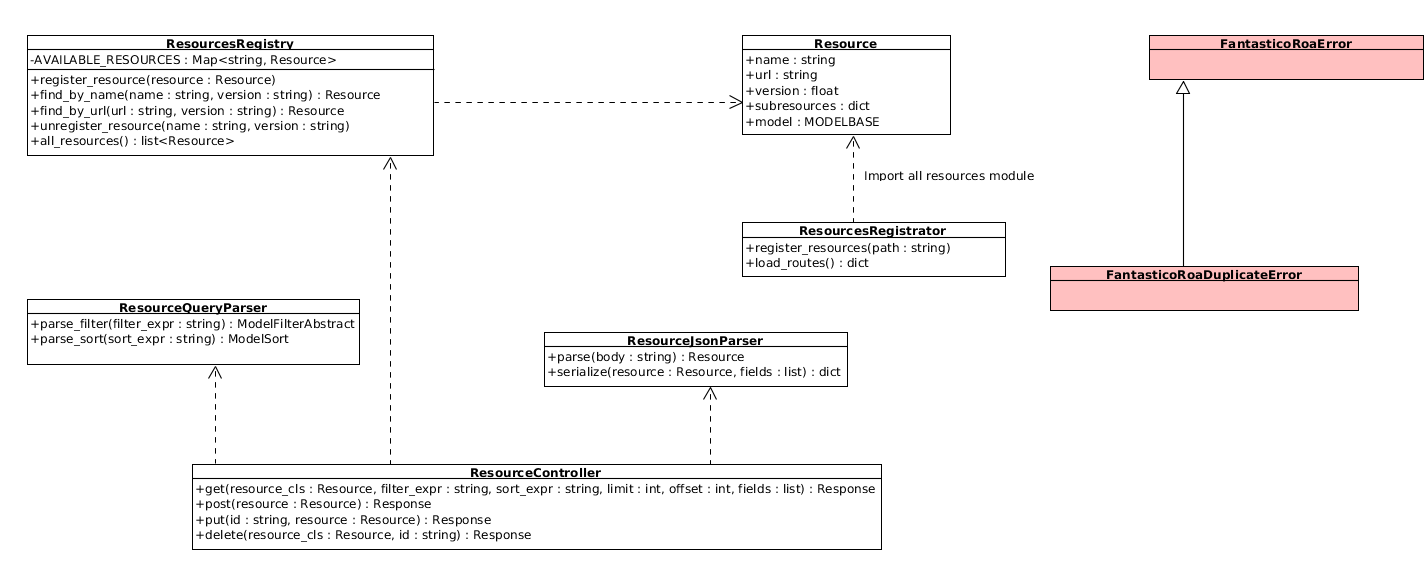
\includegraphics{roa_classes.png}

This class provides the main way for defining resources. Below you can find a very simple example for defining new resources:

\begin{Verbatim}[commandchars=\\\{\}]
\PYG{n+nd}{@Resource}\PYG{p}{(}\PYG{n}{name}\PYG{o}{=}\PYG{l+s}{\PYGZdq{}}\PYG{l+s}{app\PYGZhy{}setting}\PYG{l+s}{\PYGZdq{}}\PYG{p}{,} \PYG{n}{url}\PYG{o}{=}\PYG{l+s}{\PYGZdq{}}\PYG{l+s}{/app\PYGZhy{}settings}\PYG{l+s}{\PYGZdq{}}\PYG{p}{)}
\PYG{k}{class} \PYG{n+nc}{AppSetting}\PYG{p}{(}\PYG{n}{BASEMODEL}\PYG{p}{)}\PYG{p}{:}
    \PYG{n+nb}{id} \PYG{o}{=} \PYG{n}{Column}\PYG{p}{(}\PYG{l+s}{\PYGZdq{}}\PYG{l+s}{id}\PYG{l+s}{\PYGZdq{}}\PYG{p}{,} \PYG{n}{Integer}\PYG{p}{,} \PYG{n}{primary\PYGZus{}key}\PYG{o}{=}\PYG{n+nb+bp}{True}\PYG{p}{,} \PYG{n}{autoincrement}\PYG{o}{=}\PYG{n+nb+bp}{True}\PYG{p}{)}
    \PYG{n}{name} \PYG{o}{=} \PYG{n}{Column}\PYG{p}{(}\PYG{l+s}{\PYGZdq{}}\PYG{l+s}{name}\PYG{l+s}{\PYGZdq{}}\PYG{p}{,} \PYG{n}{String}\PYG{p}{(}\PYG{l+m+mi}{50}\PYG{p}{)}\PYG{p}{,} \PYG{n}{unique}\PYG{o}{=}\PYG{n+nb+bp}{True}\PYG{p}{,} \PYG{n}{nullable}\PYG{o}{=}\PYG{n+nb+bp}{False}\PYG{p}{)}
    \PYG{n}{value} \PYG{o}{=} \PYG{n}{Column}\PYG{p}{(}\PYG{l+s}{\PYGZdq{}}\PYG{l+s}{value}\PYG{l+s}{\PYGZdq{}}\PYG{p}{,} \PYG{n}{Text}\PYG{p}{,} \PYG{n}{nullable}\PYG{o}{=}\PYG{n+nb+bp}{False}\PYG{p}{)}

    \PYG{k}{def} \PYG{n+nf}{\PYGZus{}\PYGZus{}init\PYGZus{}\PYGZus{}}\PYG{p}{(}\PYG{n+nb+bp}{self}\PYG{p}{,} \PYG{n}{name}\PYG{o}{=}\PYG{n+nb+bp}{None}\PYG{p}{,} \PYG{n}{value}\PYG{o}{=}\PYG{n+nb+bp}{None}\PYG{p}{)}\PYG{p}{:}
       \PYG{n+nb+bp}{self}\PYG{o}{.}\PYG{n}{name} \PYG{o}{=} \PYG{n}{name}
       \PYG{n+nb+bp}{self}\PYG{o}{.}\PYG{n}{value} \PYG{o}{=} \PYG{n}{value}
\end{Verbatim}

Starting from \textbf{Fantastico} version 0.6 ROA resources support OAuth2 authorization. Because of this, resources can now be
user dependent or user independent. In order for authorization to work as expected for resources which are available only
to certain users you can use the following code snippet:

\begin{Verbatim}[commandchars=\\\{\}]
\PYG{n+nd}{@Resource}\PYG{p}{(}\PYG{n}{name}\PYG{o}{=}\PYG{l+s}{\PYGZdq{}}\PYG{l+s}{app\PYGZhy{}setting}\PYG{l+s}{\PYGZdq{}}\PYG{p}{,} \PYG{n}{url}\PYG{o}{=}\PYG{l+s}{\PYGZdq{}}\PYG{l+s}{/app\PYGZhy{}settings}\PYG{l+s}{\PYGZdq{}}\PYG{p}{,} \PYG{n}{user\PYGZus{}dependent}\PYG{o}{=}\PYG{n+nb+bp}{True}\PYG{p}{)}
\PYG{k}{class} \PYG{n+nc}{AppSetting}\PYG{p}{(}\PYG{n}{BASEMODEL}\PYG{p}{)}\PYG{p}{:}
    \PYG{n+nb}{id} \PYG{o}{=} \PYG{n}{Column}\PYG{p}{(}\PYG{l+s}{\PYGZdq{}}\PYG{l+s}{id}\PYG{l+s}{\PYGZdq{}}\PYG{p}{,} \PYG{n}{Integer}\PYG{p}{,} \PYG{n}{primary\PYGZus{}key}\PYG{o}{=}\PYG{n+nb+bp}{True}\PYG{p}{,} \PYG{n}{autoincrement}\PYG{o}{=}\PYG{n+nb+bp}{True}\PYG{p}{)}
    \PYG{n}{name} \PYG{o}{=} \PYG{n}{Column}\PYG{p}{(}\PYG{l+s}{\PYGZdq{}}\PYG{l+s}{name}\PYG{l+s}{\PYGZdq{}}\PYG{p}{,} \PYG{n}{String}\PYG{p}{(}\PYG{l+m+mi}{50}\PYG{p}{)}\PYG{p}{,} \PYG{n}{unique}\PYG{o}{=}\PYG{n+nb+bp}{True}\PYG{p}{,} \PYG{n}{nullable}\PYG{o}{=}\PYG{n+nb+bp}{False}\PYG{p}{)}
    \PYG{n}{value} \PYG{o}{=} \PYG{n}{Column}\PYG{p}{(}\PYG{l+s}{\PYGZdq{}}\PYG{l+s}{value}\PYG{l+s}{\PYGZdq{}}\PYG{p}{,} \PYG{n}{Text}\PYG{p}{,} \PYG{n}{nullable}\PYG{o}{=}\PYG{n+nb+bp}{False}\PYG{p}{)}
    \PYG{n}{user\PYGZus{}id} \PYG{o}{=} \PYG{n}{Column}\PYG{p}{(}\PYG{l+s}{\PYGZdq{}}\PYG{l+s}{user\PYGZus{}id}\PYG{l+s}{\PYGZdq{}}\PYG{p}{,} \PYG{n}{Integer}\PYG{p}{,} \PYG{n}{nullable}\PYG{o}{=}\PYG{n+nb+bp}{False}\PYG{p}{)}

    \PYG{k}{def} \PYG{n+nf}{\PYGZus{}\PYGZus{}init\PYGZus{}\PYGZus{}}\PYG{p}{(}\PYG{n+nb+bp}{self}\PYG{p}{,} \PYG{n}{name}\PYG{o}{=}\PYG{n+nb+bp}{None}\PYG{p}{,} \PYG{n}{value}\PYG{o}{=}\PYG{n+nb+bp}{None}\PYG{p}{,} \PYG{n}{user\PYGZus{}id}\PYG{o}{=}\PYG{n+nb+bp}{None}\PYG{p}{)}\PYG{p}{:}
       \PYG{n+nb+bp}{self}\PYG{o}{.}\PYG{n}{name} \PYG{o}{=} \PYG{n}{name}
       \PYG{n+nb+bp}{self}\PYG{o}{.}\PYG{n}{value} \PYG{o}{=} \PYG{n}{value}
       \PYG{n+nb+bp}{self}\PYG{o}{.}\PYG{n}{user\PYGZus{}id} \PYG{o}{=} \PYG{n}{user\PYGZus{}id}
\end{Verbatim}

If you do not define a user\_id property for user dependent resources a runtime exception is raised. In order to find out more
about OAuth2 authorization implemented into fantastico please read: {\hyperref[features/oauth2::doc]{\emph{OAUTH2}}}.
\index{model (fantastico.roa.resource\_decorator.Resource attribute)}

\begin{fulllineitems}
\phantomsection\label{features/roa/technical_summary:fantastico.roa.resource_decorator.Resource.model}\pysigline{\bfcode{model}}
This read only property holds the model of the resource.

\end{fulllineitems}

\index{name (fantastico.roa.resource\_decorator.Resource attribute)}

\begin{fulllineitems}
\phantomsection\label{features/roa/technical_summary:fantastico.roa.resource_decorator.Resource.name}\pysigline{\bfcode{name}}
This read only property holds the name of the resource.

\end{fulllineitems}

\index{subresources (fantastico.roa.resource\_decorator.Resource attribute)}

\begin{fulllineitems}
\phantomsection\label{features/roa/technical_summary:fantastico.roa.resource_decorator.Resource.subresources}\pysigline{\bfcode{subresources}}
This read only property holds the subresources of this resource. A resource can identify a subresource by one
or multiple (composite uniquely identified resources) resource attributes.

\begin{Verbatim}[commandchars=\\\{\}]
\PYG{n+nd}{@Resource}\PYG{p}{(}\PYG{n}{name}\PYG{o}{=}\PYG{l+s}{\PYGZdq{}}\PYG{l+s}{person}\PYG{l+s}{\PYGZdq{}}\PYG{p}{,} \PYG{n}{url}\PYG{o}{=}\PYG{l+s}{\PYGZdq{}}\PYG{l+s}{/persons}\PYG{l+s}{\PYGZdq{}}\PYG{p}{,} \PYG{n}{version}\PYG{o}{=}\PYG{l+m+mf}{1.0}\PYG{p}{,}
          \PYG{n}{subresources}\PYG{o}{=}\PYG{p}{\PYGZob{}}\PYG{l+s}{\PYGZdq{}}\PYG{l+s}{bill\PYGZus{}address}\PYG{l+s}{\PYGZdq{}}\PYG{p}{:} \PYG{p}{[}\PYG{l+s}{\PYGZdq{}}\PYG{l+s}{bill\PYGZus{}address\PYGZus{}id}\PYG{l+s}{\PYGZdq{}}\PYG{p}{]}\PYG{p}{,}
                        \PYG{l+s}{\PYGZdq{}}\PYG{l+s}{mail\PYGZus{}address}\PYG{l+s}{\PYGZdq{}}\PYG{p}{:} \PYG{p}{[}\PYG{l+s}{\PYGZdq{}}\PYG{l+s}{mail\PYGZus{}address\PYGZus{}id}\PYG{l+s}{\PYGZdq{}}\PYG{p}{]}\PYG{p}{,}
                        \PYG{l+s}{\PYGZdq{}}\PYG{l+s}{ship\PYGZus{}address:}\PYG{l+s}{\PYGZdq{}} \PYG{p}{[}\PYG{l+s}{\PYGZdq{}}\PYG{l+s}{ship\PYGZus{}address\PYGZus{}id}\PYG{l+s}{\PYGZdq{}}\PYG{p}{]}\PYG{p}{)}
\PYG{k}{class} \PYG{n+nc}{Person}\PYG{p}{(}\PYG{n}{BASEMODEL}\PYG{p}{)}\PYG{p}{:}
    \PYG{n+nb}{id} \PYG{o}{=} \PYG{n}{Column}\PYG{p}{(}\PYG{l+s}{\PYGZdq{}}\PYG{l+s}{id}\PYG{l+s}{\PYGZdq{}}\PYG{p}{,} \PYG{n}{Integer}\PYG{p}{,} \PYG{n}{primary\PYGZus{}key}\PYG{o}{=}\PYG{n+nb+bp}{True}\PYG{p}{,} \PYG{n}{autoincrement}\PYG{o}{=}\PYG{n+nb+bp}{True}\PYG{p}{)}
    \PYG{n}{first\PYGZus{}name} \PYG{o}{=} \PYG{n}{Column}\PYG{p}{(}\PYG{l+s}{\PYGZdq{}}\PYG{l+s}{first\PYGZus{}name}\PYG{l+s}{\PYGZdq{}}\PYG{p}{,} \PYG{n}{String}\PYG{p}{(}\PYG{l+m+mi}{80}\PYG{p}{)}\PYG{p}{)}
    \PYG{n}{last\PYGZus{}name} \PYG{o}{=} \PYG{n}{Column}\PYG{p}{(}\PYG{l+s}{\PYGZdq{}}\PYG{l+s}{last\PYGZus{}name}\PYG{l+s}{\PYGZdq{}}\PYG{p}{,} \PYG{n}{String}\PYG{p}{(}\PYG{l+m+mi}{50}\PYG{p}{)}\PYG{p}{)}
    \PYG{n}{bill\PYGZus{}address\PYGZus{}id} \PYG{o}{=} \PYG{n}{Column}\PYG{p}{(}\PYG{l+s}{\PYGZdq{}}\PYG{l+s}{bill\PYGZus{}address\PYGZus{}id}\PYG{l+s}{\PYGZdq{}}\PYG{p}{,} \PYG{n}{ForeignKey}\PYG{p}{(}\PYG{l+s}{\PYGZdq{}}\PYG{l+s}{addresses.id}\PYG{l+s}{\PYGZdq{}}\PYG{p}{)}\PYG{p}{)}
    \PYG{n}{bill\PYGZus{}address} \PYG{o}{=} \PYG{n}{relationship}\PYG{p}{(}\PYG{n}{Address}\PYG{p}{,} \PYG{n}{primaryjoin}\PYG{o}{=}\PYG{n}{bill\PYGZus{}address\PYGZus{}id} \PYG{o}{==} \PYG{n}{Address}\PYG{o}{.}\PYG{n}{id}\PYG{p}{)}
    \PYG{n}{ship\PYGZus{}address\PYGZus{}id} \PYG{o}{=} \PYG{n}{Column}\PYG{p}{(}\PYG{l+s}{\PYGZdq{}}\PYG{l+s}{ship\PYGZus{}address\PYGZus{}id}\PYG{l+s}{\PYGZdq{}}\PYG{p}{,} \PYG{n}{ForeignKey}\PYG{p}{(}\PYG{l+s}{\PYGZdq{}}\PYG{l+s}{addresses.id}\PYG{l+s}{\PYGZdq{}}\PYG{p}{)}\PYG{p}{)}
    \PYG{n}{ship\PYGZus{}address} \PYG{o}{=} \PYG{n}{relationship}\PYG{p}{(}\PYG{n}{Address}\PYG{p}{,} \PYG{n}{primaryjoin}\PYG{o}{=}\PYG{n}{ship\PYGZus{}address\PYGZus{}id} \PYG{o}{==} \PYG{n}{Address}\PYG{o}{.}\PYG{n}{id}\PYG{p}{)}
    \PYG{n}{mail\PYGZus{}address\PYGZus{}id} \PYG{o}{=} \PYG{n}{Column}\PYG{p}{(}\PYG{l+s}{\PYGZdq{}}\PYG{l+s}{ship\PYGZus{}address\PYGZus{}id}\PYG{l+s}{\PYGZdq{}}\PYG{p}{,} \PYG{n}{ForeignKey}\PYG{p}{(}\PYG{l+s}{\PYGZdq{}}\PYG{l+s}{addresses.id}\PYG{l+s}{\PYGZdq{}}\PYG{p}{)}\PYG{p}{)}
    \PYG{n}{ship\PYGZus{}address} \PYG{o}{=} \PYG{n}{relationship}\PYG{p}{(}\PYG{n}{Address}\PYG{p}{,} \PYG{n}{primaryjoin}\PYG{o}{=}\PYG{n}{mail\PYGZus{}address\PYGZus{}id} \PYG{o}{==} \PYG{n}{Address}\PYG{o}{.}\PYG{n}{id}\PYG{p}{)}
\end{Verbatim}

\end{fulllineitems}

\index{url (fantastico.roa.resource\_decorator.Resource attribute)}

\begin{fulllineitems}
\phantomsection\label{features/roa/technical_summary:fantastico.roa.resource_decorator.Resource.url}\pysigline{\bfcode{url}}
This read only property holds the url of the resource.

\end{fulllineitems}

\index{user\_dependent (fantastico.roa.resource\_decorator.Resource attribute)}

\begin{fulllineitems}
\phantomsection\label{features/roa/technical_summary:fantastico.roa.resource_decorator.Resource.user_dependent}\pysigline{\bfcode{user\_dependent}}
This read only property returns True if user is owned only by one resource and False otherwise. It is really important
to understand the impact of the property when set to True:
\begin{enumerate}
\item {} 
Every GET on resource root url will also receive a filter user\_id from access\_token == resource.model.user\_id

\item {} 
Every GET on a specific resource id will be validated also on user\_id field.

\item {} \begin{description}
\item[{Every POST for creating a new resource will automatically assign resource to user\_id found in access\_token. There is an}] \leavevmode
exception when the resource does not require create scopes.

\end{description}

\item {} 
Every PUT on a specific resource id will also check to ensure the user from the access\_token owns the resource.

\item {} 
Every DELETE on a specific resource id will also check to ensure the user from the access\_token owns the resource.

\end{enumerate}

\end{fulllineitems}

\index{validator (fantastico.roa.resource\_decorator.Resource attribute)}

\begin{fulllineitems}
\phantomsection\label{features/roa/technical_summary:fantastico.roa.resource_decorator.Resource.validator}\pysigline{\bfcode{validator}}
This property returns the validator type which must be used for this resource for creating / updating it. You can
read more about it on {\hyperref[features/roa/technical_summary:fantastico.roa.resource_validator.ResourceValidator]{\code{fantastico.roa.resource\_validator.ResourceValidator}}}.

\end{fulllineitems}

\index{version (fantastico.roa.resource\_decorator.Resource attribute)}

\begin{fulllineitems}
\phantomsection\label{features/roa/technical_summary:fantastico.roa.resource_decorator.Resource.version}\pysigline{\bfcode{version}}
This read only property holds the version of the resource.

\end{fulllineitems}


\end{fulllineitems}

\index{ResourcesRegistry (class in fantastico.roa.resources\_registry)}

\begin{fulllineitems}
\phantomsection\label{features/roa/technical_summary:fantastico.roa.resources_registry.ResourcesRegistry}\pysigline{\strong{class }\code{fantastico.roa.resources\_registry.}\bfcode{ResourcesRegistry}}
This class provide the methods for registering resources into Fantastico framework and locating them by url or name and
version. As a Developer you will not usually need access to this class.
\index{all\_resources() (fantastico.roa.resources\_registry.ResourcesRegistry method)}

\begin{fulllineitems}
\phantomsection\label{features/roa/technical_summary:fantastico.roa.resources_registry.ResourcesRegistry.all_resources}\pysiglinewithargsret{\bfcode{all\_resources}}{}{}
This method returns a list of all registered resources order by name and version. It is extremely useful for
introspecting Fantastico ROA platform.

\end{fulllineitems}

\index{available\_resources (fantastico.roa.resources\_registry.ResourcesRegistry attribute)}

\begin{fulllineitems}
\phantomsection\label{features/roa/technical_summary:fantastico.roa.resources_registry.ResourcesRegistry.available_resources}\pysigline{\bfcode{available\_resources}}
This readonly property returns the indexed resources by name.

\end{fulllineitems}

\index{available\_url\_resources (fantastico.roa.resources\_registry.ResourcesRegistry attribute)}

\begin{fulllineitems}
\phantomsection\label{features/roa/technical_summary:fantastico.roa.resources_registry.ResourcesRegistry.available_url_resources}\pysigline{\bfcode{available\_url\_resources}}
This readonly property returns the indexed resources by urk.

\end{fulllineitems}

\index{find\_by\_name() (fantastico.roa.resources\_registry.ResourcesRegistry method)}

\begin{fulllineitems}
\phantomsection\label{features/roa/technical_summary:fantastico.roa.resources_registry.ResourcesRegistry.find_by_name}\pysiglinewithargsret{\bfcode{find\_by\_name}}{\emph{name}, \emph{version='latest'}}{}
This method returns a registered resource under the given name and version.
\begin{quote}\begin{description}
\item[{Parameters}] \leavevmode\begin{itemize}
\item {} 
\textbf{name} (\emph{string}) -- The resource name.

\item {} 
\textbf{version} (\emph{string}) -- The numeric version of the resource or \textbf{latest}.

\end{itemize}

\item[{Returns}] \leavevmode
The resource found or None.

\item[{Return type}] \leavevmode
{\hyperref[features/roa/technical_summary:fantastico.roa.resource_decorator.Resource]{\code{fantastico.roa.resource\_decorator.Resource}}}

\end{description}\end{quote}

\end{fulllineitems}

\index{find\_by\_url() (fantastico.roa.resources\_registry.ResourcesRegistry method)}

\begin{fulllineitems}
\phantomsection\label{features/roa/technical_summary:fantastico.roa.resources_registry.ResourcesRegistry.find_by_url}\pysiglinewithargsret{\bfcode{find\_by\_url}}{\emph{url}, \emph{version='latest'}}{}
This method returns a registered resource under the given url and version.
\begin{quote}\begin{description}
\item[{Parameters}] \leavevmode\begin{itemize}
\item {} 
\textbf{name} (\emph{string}) -- The resource name.

\item {} 
\textbf{version} (\emph{string}) -- The numeric version of the resource or \textbf{latest}.

\end{itemize}

\item[{Returns}] \leavevmode
The resource found or None.

\item[{Return type}] \leavevmode
{\hyperref[features/roa/technical_summary:fantastico.roa.resource_decorator.Resource]{\code{fantastico.roa.resource\_decorator.Resource}}}

\end{description}\end{quote}

\end{fulllineitems}

\index{register\_resource() (fantastico.roa.resources\_registry.ResourcesRegistry method)}

\begin{fulllineitems}
\phantomsection\label{features/roa/technical_summary:fantastico.roa.resources_registry.ResourcesRegistry.register_resource}\pysiglinewithargsret{\bfcode{register\_resource}}{\emph{resource}}{}
This method register a new resource into Fantastico framework. It first checks against name, url and version collision
in order to detect as early as possible errors with the current defined resources.
\begin{quote}\begin{description}
\item[{Parameters}] \leavevmode
\textbf{resource} ({\hyperref[features/roa/technical_summary:fantastico.roa.resource_decorator.Resource]{\code{fantastico.roa.resource\_decorator.Resource}}}) -- The resource instance we want to register into Fantastico ROA registry.

\item[{Raises {\hyperref[features/roa/technical_summary:fantastico.roa.roa_exceptions.FantasticoRoaDuplicateError]{fantastico.roa.roa\_exceptions.FantasticoRoaDuplicateError}}}] \leavevmode

This exception is raised when:
\begin{itemize}
\item {} 
resource name and version already registered.

\item {} 
resource url already registered.

\end{itemize}


\end{description}\end{quote}

\end{fulllineitems}

\index{unregister\_resource() (fantastico.roa.resources\_registry.ResourcesRegistry method)}

\begin{fulllineitems}
\phantomsection\label{features/roa/technical_summary:fantastico.roa.resources_registry.ResourcesRegistry.unregister_resource}\pysiglinewithargsret{\bfcode{unregister\_resource}}{\emph{name}, \emph{version}}{}
This method unregister a resource version. If the given resource is not found no exception is raised. Once a resource
is unregistered latest version is recalculated. The resource is completely removed from AVAILABLE\_RESOURCES and
AVAILABLE\_URLS dictionaries.
\begin{quote}\begin{description}
\item[{Parameters}] \leavevmode\begin{itemize}
\item {} 
\textbf{name} (\emph{string}) -- Resource name.

\item {} 
\textbf{version} (\emph{float}) -- Resource version. If you specify \textbf{latest} it will have no effect.

\end{itemize}

\end{description}\end{quote}

\end{fulllineitems}


\end{fulllineitems}

\index{ResourcesRegistrator (class in fantastico.roa.resources\_registrator)}

\begin{fulllineitems}
\phantomsection\label{features/roa/technical_summary:fantastico.roa.resources_registrator.ResourcesRegistrator}\pysiglinewithargsret{\strong{class }\code{fantastico.roa.resources\_registrator.}\bfcode{ResourcesRegistrator}}{\emph{settings\_facade}, \emph{file\_patterns=None}, \emph{folder\_pattern=None}}{}
This class provides the algorithm for registering all defined resources. Resources discovered by this class are decorated
by {\hyperref[features/roa/technical_summary:fantastico.roa.resource_decorator.Resource]{\code{fantastico.roa.resource\_decorator.Resource}}}. In the constructor of this class you can define special naming
convention for discovered resources (through regex). Default behavior is to scan only in models folder / subfolders in all
available files.

In addition this class is also designed to be a route provider. This guarantees that at start time, all resources will be
registered correctly.
\index{load\_routes() (fantastico.roa.resources\_registrator.ResourcesRegistrator method)}

\begin{fulllineitems}
\phantomsection\label{features/roa/technical_summary:fantastico.roa.resources_registrator.ResourcesRegistrator.load_routes}\pysiglinewithargsret{\bfcode{load\_routes}}{}{}
This method simple triggers resources registration and returns empty routes. Using this mechanism guarantees that
routing engine will also discover ROA resources.

\end{fulllineitems}

\index{register\_resources() (fantastico.roa.resources\_registrator.ResourcesRegistrator method)}

\begin{fulllineitems}
\phantomsection\label{features/roa/technical_summary:fantastico.roa.resources_registrator.ResourcesRegistrator.register_resources}\pysiglinewithargsret{\bfcode{register\_resources}}{\emph{path}}{}
This method scans all files and folders from the given path, match the filenames against registered file patterns
and import all ROA resources.

\end{fulllineitems}


\end{fulllineitems}

\index{RoaDiscoveryController (class in fantastico.contrib.roa\_discovery.discovery\_controller)}

\begin{fulllineitems}
\phantomsection\label{features/roa/technical_summary:fantastico.contrib.roa_discovery.discovery_controller.RoaDiscoveryController}\pysiglinewithargsret{\strong{class }\code{fantastico.contrib.roa\_discovery.discovery\_controller.}\bfcode{RoaDiscoveryController}}{\emph{settings\_facade}, \emph{registry\_cls=None}}{}
This class provides the routes for introspecting Fantastico registered resources through ROA. It is extremely useful
to surf using your browser and to not be required to hardcode links in your code. Typically, you will want to code your
client side applications against resources name and you are going to use this controller to find the location of those
records.

By default, all ROA resources are mapped on \textbf{/api/} relative to current project root. You can easily change this behavior
by modifying the settings of your application ({\hyperref[get_started/settings:fantastico.settings.BasicSettings]{\code{fantastico.settings.BasicSettings}}} - property \textbf{roa\_api\_url})
\index{handle\_list\_resources\_options() (fantastico.contrib.roa\_discovery.discovery\_controller.RoaDiscoveryController method)}

\begin{fulllineitems}
\phantomsection\label{features/roa/technical_summary:fantastico.contrib.roa_discovery.discovery_controller.RoaDiscoveryController.handle_list_resources_options}\pysiglinewithargsret{\bfcode{handle\_list\_resources\_options}}{\emph{*args}, \emph{**kwargs}}{}
This method handles all OPTIONS cors requests coming for resources registry listing.

\end{fulllineitems}

\index{list\_registered\_resources() (fantastico.contrib.roa\_discovery.discovery\_controller.RoaDiscoveryController method)}

\begin{fulllineitems}
\phantomsection\label{features/roa/technical_summary:fantastico.contrib.roa_discovery.discovery_controller.RoaDiscoveryController.list_registered_resources}\pysiglinewithargsret{\bfcode{list\_registered\_resources}}{\emph{*args}, \emph{**kwargs}}{}
This method list all registered resources as well as a link to their entry point.

\begin{Verbatim}[commandchars=\\\{\}]
\PYG{c+c1}{// ROA api is mapped on a subdomain: roa.fantasticoproject.com}
\PYG{c+c1}{// listing is done by GET http://fantasticoproject.com/roa/resources HTTP/1.1}

\PYG{p}{\PYGZob{}}
    \PYG{l+s+s2}{\PYGZdq{}Person\PYGZdq{}}\PYG{o}{:} \PYG{p}{\PYGZob{}}\PYG{l+m+mf}{1.0} \PYG{o}{:} \PYG{l+s+s2}{\PYGZdq{}http://roa.fantasticoproject.com/1.0/persons\PYGZdq{}}\PYG{p}{,}
               \PYG{l+s+s2}{\PYGZdq{}latest\PYGZdq{}}\PYG{o}{:} \PYG{l+s+s2}{\PYGZdq{}http://roa.fantasticoproject.com/latest/persons\PYGZdq{}}\PYG{p}{\PYGZcb{}}\PYG{p}{,}
    \PYG{l+s+s2}{\PYGZdq{}Address\PYGZdq{}}\PYG{o}{:} \PYG{p}{\PYGZob{}}\PYG{l+m+mf}{1.0} \PYG{o}{:} \PYG{l+s+s2}{\PYGZdq{}http://roa.fantasticoproject.com/1.0/addresses\PYGZdq{}}\PYG{p}{,}
                \PYG{l+m+mf}{2.0} \PYG{o}{:} \PYG{l+s+s2}{\PYGZdq{}http://roa.fantasticoproject.com/2.0/addresses\PYGZdq{}}\PYG{p}{,}
                \PYG{l+s+s2}{\PYGZdq{}latest\PYGZdq{}}\PYG{o}{:} \PYG{l+s+s2}{\PYGZdq{}http://roa.fantasticoproject.com/latest/addresses\PYGZdq{}}\PYG{p}{\PYGZcb{}}
\PYG{p}{\PYGZcb{}}
\end{Verbatim}

\begin{Verbatim}[commandchars=\\\{\}]
\PYG{c+c1}{// ROA api is mapped on a relative path of the project: http://fantasticoproject.com/api/}
\PYG{c+c1}{// listing is done by GET http://fantasticoproject.com/roa/resources HTTP/1.1}

\PYG{p}{\PYGZob{}}
    \PYG{l+s+s2}{\PYGZdq{}Person\PYGZdq{}}\PYG{o}{:} \PYG{p}{\PYGZob{}}\PYG{l+m+mf}{1.0} \PYG{o}{:} \PYG{l+s+s2}{\PYGZdq{}http://fantasticoproject.com/api/1.0/persons\PYGZdq{}}\PYG{p}{,}
               \PYG{l+s+s2}{\PYGZdq{}latest\PYGZdq{}}\PYG{o}{:} \PYG{l+s+s2}{\PYGZdq{}http://roa.fantasticoproject.com/api/latest/persons\PYGZdq{}}\PYG{p}{\PYGZcb{}}\PYG{p}{,}
    \PYG{l+s+s2}{\PYGZdq{}Address\PYGZdq{}}\PYG{o}{:} \PYG{p}{\PYGZob{}}\PYG{l+m+mf}{1.0} \PYG{o}{:} \PYG{l+s+s2}{\PYGZdq{}http://roa.fantasticoproject.com/api/1.0/addresses\PYGZdq{}}\PYG{p}{,}
                \PYG{l+m+mf}{2.0} \PYG{o}{:} \PYG{l+s+s2}{\PYGZdq{}http://roa.fantasticoproject.com/api/2.0/addresses\PYGZdq{}}\PYG{p}{,}
                \PYG{l+s+s2}{\PYGZdq{}latest\PYGZdq{}}\PYG{o}{:} \PYG{l+s+s2}{\PYGZdq{}http://roa.fantasticoproject.com/api/latest/addresses\PYGZdq{}}\PYG{p}{\PYGZcb{}}
\PYG{p}{\PYGZcb{}}
\end{Verbatim}

\end{fulllineitems}


\end{fulllineitems}

\index{QueryParser (class in fantastico.roa.query\_parser)}

\begin{fulllineitems}
\phantomsection\label{features/roa/technical_summary:fantastico.roa.query_parser.QueryParser}\pysigline{\strong{class }\code{fantastico.roa.query\_parser.}\bfcode{QueryParser}}
This class provides ROA query parser functionality. It provides methods for transforming filter and sorting expressions
({\hyperref[features/roa/rest_standard::doc]{\emph{REST API standard}}}) into mvc filters ({\hyperref[features/mvc::doc]{\emph{Model View Controller}}}).
\index{parse\_filter() (fantastico.roa.query\_parser.QueryParser method)}

\begin{fulllineitems}
\phantomsection\label{features/roa/technical_summary:fantastico.roa.query_parser.QueryParser.parse_filter}\pysiglinewithargsret{\bfcode{parse\_filter}}{\emph{filter\_expr}, \emph{model}}{}
This method transform the given filter expression into mvc filters.
\begin{quote}\begin{description}
\item[{Parameters}] \leavevmode\begin{itemize}
\item {} 
\textbf{filter\_expr} -- The filter string expression we want to convert to query objects.

\item {} 
\textbf{model} -- The model used to describe the resource on which the requests are done.

\end{itemize}

\item[{Returns}] \leavevmode
The newly created mvc query object.

\item[{Return type}] \leavevmode
{\hyperref[features/mvc:fantastico.mvc.models.model_filter.ModelFilterAbstract]{\code{fantastico.mvc.models.model\_filter.ModelFilterAbstract}}}

\end{description}\end{quote}

\end{fulllineitems}

\index{parse\_sort() (fantastico.roa.query\_parser.QueryParser method)}

\begin{fulllineitems}
\phantomsection\label{features/roa/technical_summary:fantastico.roa.query_parser.QueryParser.parse_sort}\pysiglinewithargsret{\bfcode{parse\_sort}}{\emph{sort\_expr}, \emph{model}}{}
This method transform the given sort expression into mvc sort filter.
\begin{quote}\begin{description}
\item[{Parameters}] \leavevmode\begin{itemize}
\item {} 
\textbf{filter\_expr} -- The filter string expression we want to convert to query objects.

\item {} 
\textbf{model} -- The model used to describe the resource on which the requests are done.

\end{itemize}

\item[{Returns}] \leavevmode
The newly created mvc query object.

\item[{Return type}] \leavevmode
{\hyperref[features/mvc:fantastico.mvc.models.model_sort.ModelSort]{\code{fantastico.mvc.models.model\_sort.ModelSort}}}

\end{description}\end{quote}

\end{fulllineitems}


\end{fulllineitems}

\index{QueryParserOperation (class in fantastico.roa.query\_parser\_operations)}

\begin{fulllineitems}
\phantomsection\label{features/roa/technical_summary:fantastico.roa.query_parser_operations.QueryParserOperation}\pysiglinewithargsret{\strong{class }\code{fantastico.roa.query\_parser\_operations.}\bfcode{QueryParserOperation}}{\emph{parser}}{}
This class defines the contract for a query parser operation.
\index{add\_argument() (fantastico.roa.query\_parser\_operations.QueryParserOperation method)}

\begin{fulllineitems}
\phantomsection\label{features/roa/technical_summary:fantastico.roa.query_parser_operations.QueryParserOperation.add_argument}\pysiglinewithargsret{\bfcode{add\_argument}}{\emph{argument}}{}
This method add a new argument to the parser operation.

\end{fulllineitems}

\index{build\_filter() (fantastico.roa.query\_parser\_operations.QueryParserOperation method)}

\begin{fulllineitems}
\phantomsection\label{features/roa/technical_summary:fantastico.roa.query_parser_operations.QueryParserOperation.build_filter}\pysiglinewithargsret{\bfcode{build\_filter}}{\emph{model}}{}
This method builds the model filter (\code{fantastico.mvc.models.model\_filter.ModelFilter}).

\end{fulllineitems}

\index{get\_filter() (fantastico.roa.query\_parser\_operations.QueryParserOperation method)}

\begin{fulllineitems}
\phantomsection\label{features/roa/technical_summary:fantastico.roa.query_parser_operations.QueryParserOperation.get_filter}\pysiglinewithargsret{\bfcode{get\_filter}}{\emph{model}}{}
This method validates the current operation and build the filter.

\end{fulllineitems}

\index{get\_grammar\_rules() (fantastico.roa.query\_parser\_operations.QueryParserOperation method)}

\begin{fulllineitems}
\phantomsection\label{features/roa/technical_summary:fantastico.roa.query_parser_operations.QueryParserOperation.get_grammar_rules}\pysiglinewithargsret{\bfcode{get\_grammar\_rules}}{}{}
This method returns the rules required to interpret this operation.

\begin{Verbatim}[commandchars=\\\{\}]
\PYG{k}{return} \PYG{p}{\PYGZob{}}
            \PYG{l+s}{\PYGZdq{}}\PYG{l+s}{(}\PYG{l+s}{\PYGZdq{}}\PYG{p}{:} \PYG{p}{[}\PYG{p}{(}\PYG{n+nb+bp}{self}\PYG{o}{.}\PYG{n}{TERM}\PYG{p}{,} \PYG{l+s}{\PYGZdq{}}\PYG{l+s}{(}\PYG{l+s}{\PYGZdq{}}\PYG{p}{)}\PYG{p}{,} \PYG{p}{(}\PYG{n+nb+bp}{self}\PYG{o}{.}\PYG{n}{RULE}\PYG{p}{,} \PYG{n+nb+bp}{self}\PYG{o}{.}\PYG{n}{REGEX\PYGZus{}TEXT}\PYG{p}{)}\PYG{p}{,} \PYG{p}{(}\PYG{n+nb+bp}{self}\PYG{o}{.}\PYG{n}{RULE}\PYG{p}{,} \PYG{l+s}{\PYGZdq{}}\PYG{l+s}{,}\PYG{l+s}{\PYGZdq{}}\PYG{p}{)}\PYG{p}{,} \PYG{p}{(}\PYG{n+nb+bp}{self}\PYG{o}{.}\PYG{n}{RULE}\PYG{p}{,} \PYG{n+nb+bp}{self}\PYG{o}{.}\PYG{n}{REGEX\PYGZus{}TEXT}\PYG{p}{)}\PYG{p}{,}
                  \PYG{p}{(}\PYG{n+nb+bp}{self}\PYG{o}{.}\PYG{n}{RULE}\PYG{p}{,} \PYG{l+s}{\PYGZdq{}}\PYG{l+s}{)}\PYG{l+s}{\PYGZdq{}}\PYG{p}{)}\PYG{p}{]}\PYG{p}{,}
       \PYG{p}{\PYGZcb{}}
\end{Verbatim}

Grammar rules simply describe the tokens which come after operator + symbol. For instance, \textbf{eq(} is followed by two
comma separated arguments.

\end{fulllineitems}

\index{get\_grammar\_table() (fantastico.roa.query\_parser\_operations.QueryParserOperation method)}

\begin{fulllineitems}
\phantomsection\label{features/roa/technical_summary:fantastico.roa.query_parser_operations.QueryParserOperation.get_grammar_table}\pysiglinewithargsret{\bfcode{get\_grammar\_table}}{\emph{new\_mixin}}{}
This method returns a dictionary describing the operator + symbol rule and action.

\begin{Verbatim}[commandchars=\\\{\}]
\PYG{k}{return} \PYG{p}{\PYGZob{}}
            \PYG{l+s}{\PYGZdq{}}\PYG{l+s}{(}\PYG{l+s}{\PYGZdq{}}\PYG{p}{:} \PYG{p}{(}\PYG{l+s}{\PYGZdq{}}\PYG{l+s}{eq}\PYG{l+s}{\PYGZdq{}}\PYG{p}{,} \PYG{l+s}{\PYGZdq{}}\PYG{l+s}{(}\PYG{l+s}{\PYGZdq{}}\PYG{p}{,} \PYG{k}{lambda}\PYG{p}{:} \PYG{n}{new\PYGZus{}mixin}\PYG{p}{(}\PYG{n}{QueryParserOperationBinaryEq}\PYG{p}{)}\PYG{p}{)}\PYG{p}{,}
            \PYG{l+s}{\PYGZdq{}}\PYG{l+s}{)}\PYG{l+s}{\PYGZdq{}}\PYG{p}{:} \PYG{n+nb+bp}{None}
       \PYG{p}{\PYGZcb{}}
\end{Verbatim}
\begin{quote}\begin{description}
\item[{Parameters}] \leavevmode
\textbf{new\_mixin} (\emph{function}) -- New mixin described a factory method required to correctly pass current operation to parser.

\item[{Returns}] \leavevmode
A dictionary describing the grammar table for this operator.

\end{description}\end{quote}

\end{fulllineitems}

\index{get\_token() (fantastico.roa.query\_parser\_operations.QueryParserOperation method)}

\begin{fulllineitems}
\phantomsection\label{features/roa/technical_summary:fantastico.roa.query_parser_operations.QueryParserOperation.get_token}\pysiglinewithargsret{\bfcode{get\_token}}{}{}
This method returns the token which maps on this operation.

\end{fulllineitems}

\index{validate() (fantastico.roa.query\_parser\_operations.QueryParserOperation method)}

\begin{fulllineitems}
\phantomsection\label{features/roa/technical_summary:fantastico.roa.query_parser_operations.QueryParserOperation.validate}\pysiglinewithargsret{\bfcode{validate}}{\emph{model}}{}
This method validates the given operation and argument in order to ensure a filter can be built.
\begin{quote}\begin{description}
\item[{Raises {\hyperref[features/roa/technical_summary:fantastico.roa.query_parser_exceptions.QueryParserOperationInvalidError]{fantastico.roa.query\_parser\_exceptions.QueryParserOperationInvalidError}}}] \leavevmode
Whenever the current operation attributes are invalid.

\end{description}\end{quote}

\end{fulllineitems}


\end{fulllineitems}

\index{QueryParserOperationBinary (class in fantastico.roa.query\_parser\_operations)}

\begin{fulllineitems}
\phantomsection\label{features/roa/technical_summary:fantastico.roa.query_parser_operations.QueryParserOperationBinary}\pysiglinewithargsret{\strong{class }\code{fantastico.roa.query\_parser\_operations.}\bfcode{QueryParserOperationBinary}}{\emph{parser}}{}
This class provides the validation / build logic for binary operations.
\index{build\_filter() (fantastico.roa.query\_parser\_operations.QueryParserOperationBinary method)}

\begin{fulllineitems}
\phantomsection\label{features/roa/technical_summary:fantastico.roa.query_parser_operations.QueryParserOperationBinary.build_filter}\pysiglinewithargsret{\bfcode{build\_filter}}{\emph{model}}{}
This method builds a binary filter.

\end{fulllineitems}

\index{get\_grammar\_rules() (fantastico.roa.query\_parser\_operations.QueryParserOperationBinary method)}

\begin{fulllineitems}
\phantomsection\label{features/roa/technical_summary:fantastico.roa.query_parser_operations.QueryParserOperationBinary.get_grammar_rules}\pysiglinewithargsret{\bfcode{get\_grammar\_rules}}{}{}
This method returns the grammar rules supported by binary operators.

\end{fulllineitems}

\index{get\_grammar\_table() (fantastico.roa.query\_parser\_operations.QueryParserOperationBinary method)}

\begin{fulllineitems}
\phantomsection\label{features/roa/technical_summary:fantastico.roa.query_parser_operations.QueryParserOperationBinary.get_grammar_table}\pysiglinewithargsret{\bfcode{get\_grammar\_table}}{\emph{new\_mixin}}{}
The grammar table supported by binary operators.

\end{fulllineitems}

\index{validate() (fantastico.roa.query\_parser\_operations.QueryParserOperationBinary method)}

\begin{fulllineitems}
\phantomsection\label{features/roa/technical_summary:fantastico.roa.query_parser_operations.QueryParserOperationBinary.validate}\pysiglinewithargsret{\bfcode{validate}}{\emph{model}}{}
This method ensures that three arguments were passed.

\end{fulllineitems}


\end{fulllineitems}

\index{QueryParserOperationBinaryEq (class in fantastico.roa.query\_parser\_operations)}

\begin{fulllineitems}
\phantomsection\label{features/roa/technical_summary:fantastico.roa.query_parser_operations.QueryParserOperationBinaryEq}\pysiglinewithargsret{\strong{class }\code{fantastico.roa.query\_parser\_operations.}\bfcode{QueryParserOperationBinaryEq}}{\emph{parser}}{}
This class provides the eq operator which can compare two arguments for equality.
\index{get\_token() (fantastico.roa.query\_parser\_operations.QueryParserOperationBinaryEq method)}

\begin{fulllineitems}
\phantomsection\label{features/roa/technical_summary:fantastico.roa.query_parser_operations.QueryParserOperationBinaryEq.get_token}\pysiglinewithargsret{\bfcode{get\_token}}{}{}
This method returns the equality token supported by ROA query language.

\end{fulllineitems}


\end{fulllineitems}

\index{QueryParserOperationBinaryGt (class in fantastico.roa.query\_parser\_operations)}

\begin{fulllineitems}
\phantomsection\label{features/roa/technical_summary:fantastico.roa.query_parser_operations.QueryParserOperationBinaryGt}\pysiglinewithargsret{\strong{class }\code{fantastico.roa.query\_parser\_operations.}\bfcode{QueryParserOperationBinaryGt}}{\emph{parser}}{}
This class provides the gt operator which can compare two arguments for greater than relation.
\index{get\_token() (fantastico.roa.query\_parser\_operations.QueryParserOperationBinaryGt method)}

\begin{fulllineitems}
\phantomsection\label{features/roa/technical_summary:fantastico.roa.query_parser_operations.QueryParserOperationBinaryGt.get_token}\pysiglinewithargsret{\bfcode{get\_token}}{}{}
This method returns the greater than token supported by ROA query language.

\end{fulllineitems}


\end{fulllineitems}

\index{QueryParserOperationBinaryGe (class in fantastico.roa.query\_parser\_operations)}

\begin{fulllineitems}
\phantomsection\label{features/roa/technical_summary:fantastico.roa.query_parser_operations.QueryParserOperationBinaryGe}\pysiglinewithargsret{\strong{class }\code{fantastico.roa.query\_parser\_operations.}\bfcode{QueryParserOperationBinaryGe}}{\emph{parser}}{}
This class provides the ge operator which can compare two arguments for greater or equal than relation.
\index{get\_token() (fantastico.roa.query\_parser\_operations.QueryParserOperationBinaryGe method)}

\begin{fulllineitems}
\phantomsection\label{features/roa/technical_summary:fantastico.roa.query_parser_operations.QueryParserOperationBinaryGe.get_token}\pysiglinewithargsret{\bfcode{get\_token}}{}{}
This method returns the greater equals token supported by ROA query language.

\end{fulllineitems}


\end{fulllineitems}

\index{QueryParserOperationBinaryLt (class in fantastico.roa.query\_parser\_operations)}

\begin{fulllineitems}
\phantomsection\label{features/roa/technical_summary:fantastico.roa.query_parser_operations.QueryParserOperationBinaryLt}\pysiglinewithargsret{\strong{class }\code{fantastico.roa.query\_parser\_operations.}\bfcode{QueryParserOperationBinaryLt}}{\emph{parser}}{}
This class provides the lt operator which can compare two arguments for less than relation.
\index{get\_token() (fantastico.roa.query\_parser\_operations.QueryParserOperationBinaryLt method)}

\begin{fulllineitems}
\phantomsection\label{features/roa/technical_summary:fantastico.roa.query_parser_operations.QueryParserOperationBinaryLt.get_token}\pysiglinewithargsret{\bfcode{get\_token}}{}{}
This method returns the less than token supported by ROA query language.

\end{fulllineitems}


\end{fulllineitems}

\index{QueryParserOperationBinaryLe (class in fantastico.roa.query\_parser\_operations)}

\begin{fulllineitems}
\phantomsection\label{features/roa/technical_summary:fantastico.roa.query_parser_operations.QueryParserOperationBinaryLe}\pysiglinewithargsret{\strong{class }\code{fantastico.roa.query\_parser\_operations.}\bfcode{QueryParserOperationBinaryLe}}{\emph{parser}}{}
This class provides the le operator which can compare two arguments for less or equal than relation.
\index{get\_token() (fantastico.roa.query\_parser\_operations.QueryParserOperationBinaryLe method)}

\begin{fulllineitems}
\phantomsection\label{features/roa/technical_summary:fantastico.roa.query_parser_operations.QueryParserOperationBinaryLe.get_token}\pysiglinewithargsret{\bfcode{get\_token}}{}{}
This method returns the less equal than token supported by ROA query language.

\end{fulllineitems}


\end{fulllineitems}

\index{QueryParserOperationBinaryIn (class in fantastico.roa.query\_parser\_operations)}

\begin{fulllineitems}
\phantomsection\label{features/roa/technical_summary:fantastico.roa.query_parser_operations.QueryParserOperationBinaryIn}\pysiglinewithargsret{\strong{class }\code{fantastico.roa.query\_parser\_operations.}\bfcode{QueryParserOperationBinaryIn}}{\emph{parser}}{}
This class provides the in operator which can compare a value with a possible list of values.
\index{get\_token() (fantastico.roa.query\_parser\_operations.QueryParserOperationBinaryIn method)}

\begin{fulllineitems}
\phantomsection\label{features/roa/technical_summary:fantastico.roa.query_parser_operations.QueryParserOperationBinaryIn.get_token}\pysiglinewithargsret{\bfcode{get\_token}}{}{}
This method returns in token supported by ROA query language.

\end{fulllineitems}


\end{fulllineitems}

\index{QueryParserOperationBinaryLike (class in fantastico.roa.query\_parser\_operations)}

\begin{fulllineitems}
\phantomsection\label{features/roa/technical_summary:fantastico.roa.query_parser_operations.QueryParserOperationBinaryLike}\pysiglinewithargsret{\strong{class }\code{fantastico.roa.query\_parser\_operations.}\bfcode{QueryParserOperationBinaryLike}}{\emph{parser}}{}
This class provides the like operator which can compare two arguments for similarity.
\index{get\_token() (fantastico.roa.query\_parser\_operations.QueryParserOperationBinaryLike method)}

\begin{fulllineitems}
\phantomsection\label{features/roa/technical_summary:fantastico.roa.query_parser_operations.QueryParserOperationBinaryLike.get_token}\pysiglinewithargsret{\bfcode{get\_token}}{}{}
This method returns like token supported by ROA query language.

\end{fulllineitems}


\end{fulllineitems}

\index{QueryParserOperationCompound (class in fantastico.roa.query\_parser\_operations)}

\begin{fulllineitems}
\phantomsection\label{features/roa/technical_summary:fantastico.roa.query_parser_operations.QueryParserOperationCompound}\pysiglinewithargsret{\strong{class }\code{fantastico.roa.query\_parser\_operations.}\bfcode{QueryParserOperationCompound}}{\emph{parser}, \emph{compound\_filter\_cls=None}}{}
This class provides the parser for compound filter or. It will recursively parse each argument and in the end will return
a compatible \code{fantastico.mvc.model\_filter\_compound.ModelFilterCompound}. Each concrete class must specify the
compound filter type to use.
\index{build\_filter() (fantastico.roa.query\_parser\_operations.QueryParserOperationCompound method)}

\begin{fulllineitems}
\phantomsection\label{features/roa/technical_summary:fantastico.roa.query_parser_operations.QueryParserOperationCompound.build_filter}\pysiglinewithargsret{\bfcode{build\_filter}}{\emph{model}}{}
This method builds the compound filter based on the parsed arguments of this operation.

\end{fulllineitems}

\index{get\_grammar\_rules() (fantastico.roa.query\_parser\_operations.QueryParserOperationCompound method)}

\begin{fulllineitems}
\phantomsection\label{features/roa/technical_summary:fantastico.roa.query_parser_operations.QueryParserOperationCompound.get_grammar_rules}\pysiglinewithargsret{\bfcode{get\_grammar\_rules}}{}{}
This method returns the grammar rules supported by binary operators.

\end{fulllineitems}

\index{get\_grammar\_table() (fantastico.roa.query\_parser\_operations.QueryParserOperationCompound method)}

\begin{fulllineitems}
\phantomsection\label{features/roa/technical_summary:fantastico.roa.query_parser_operations.QueryParserOperationCompound.get_grammar_table}\pysiglinewithargsret{\bfcode{get\_grammar\_table}}{\emph{new\_mixin}}{}
The grammar table supported by binary operators.

\end{fulllineitems}

\index{validate() (fantastico.roa.query\_parser\_operations.QueryParserOperationCompound method)}

\begin{fulllineitems}
\phantomsection\label{features/roa/technical_summary:fantastico.roa.query_parser_operations.QueryParserOperationCompound.validate}\pysiglinewithargsret{\bfcode{validate}}{\emph{model}}{}
This method validates all arguments passed to this compound filter.

\end{fulllineitems}


\end{fulllineitems}

\index{QueryParserOperationOr (class in fantastico.roa.query\_parser\_operations)}

\begin{fulllineitems}
\phantomsection\label{features/roa/technical_summary:fantastico.roa.query_parser_operations.QueryParserOperationOr}\pysiglinewithargsret{\strong{class }\code{fantastico.roa.query\_parser\_operations.}\bfcode{QueryParserOperationOr}}{\emph{parser}}{}
This class provides a query parser for \textbf{or} compound filtering.
\index{get\_token() (fantastico.roa.query\_parser\_operations.QueryParserOperationOr method)}

\begin{fulllineitems}
\phantomsection\label{features/roa/technical_summary:fantastico.roa.query_parser_operations.QueryParserOperationOr.get_token}\pysiglinewithargsret{\bfcode{get\_token}}{}{}
This method returns or compound token for ROA query language.

\end{fulllineitems}


\end{fulllineitems}

\index{QueryParserOperationAnd (class in fantastico.roa.query\_parser\_operations)}

\begin{fulllineitems}
\phantomsection\label{features/roa/technical_summary:fantastico.roa.query_parser_operations.QueryParserOperationAnd}\pysiglinewithargsret{\strong{class }\code{fantastico.roa.query\_parser\_operations.}\bfcode{QueryParserOperationAnd}}{\emph{parser}}{}
This class provides a query parser for \textbf{and} compound filtering.
\index{get\_token() (fantastico.roa.query\_parser\_operations.QueryParserOperationAnd method)}

\begin{fulllineitems}
\phantomsection\label{features/roa/technical_summary:fantastico.roa.query_parser_operations.QueryParserOperationAnd.get_token}\pysiglinewithargsret{\bfcode{get\_token}}{}{}
This method returns and compound token for ROA query language.

\end{fulllineitems}


\end{fulllineitems}

\index{QueryParserOperationSort (class in fantastico.roa.query\_parser\_operations)}

\begin{fulllineitems}
\phantomsection\label{features/roa/technical_summary:fantastico.roa.query_parser_operations.QueryParserOperationSort}\pysiglinewithargsret{\strong{class }\code{fantastico.roa.query\_parser\_operations.}\bfcode{QueryParserOperationSort}}{\emph{parser}, \emph{sort\_dir=None}}{}
This class provides base support for sort operations: asc / desc.
\index{build\_filter() (fantastico.roa.query\_parser\_operations.QueryParserOperationSort method)}

\begin{fulllineitems}
\phantomsection\label{features/roa/technical_summary:fantastico.roa.query_parser_operations.QueryParserOperationSort.build_filter}\pysiglinewithargsret{\bfcode{build\_filter}}{\emph{model}}{}
This method builds the sorting model.

\end{fulllineitems}

\index{get\_grammar\_rules() (fantastico.roa.query\_parser\_operations.QueryParserOperationSort method)}

\begin{fulllineitems}
\phantomsection\label{features/roa/technical_summary:fantastico.roa.query_parser_operations.QueryParserOperationSort.get_grammar_rules}\pysiglinewithargsret{\bfcode{get\_grammar\_rules}}{}{}
This method returns the grammar rules supported by binary operators.

\end{fulllineitems}

\index{get\_grammar\_table() (fantastico.roa.query\_parser\_operations.QueryParserOperationSort method)}

\begin{fulllineitems}
\phantomsection\label{features/roa/technical_summary:fantastico.roa.query_parser_operations.QueryParserOperationSort.get_grammar_table}\pysiglinewithargsret{\bfcode{get\_grammar\_table}}{\emph{new\_mixin}}{}
The grammar table supported by binary operators.

\end{fulllineitems}

\index{validate() (fantastico.roa.query\_parser\_operations.QueryParserOperationSort method)}

\begin{fulllineitems}
\phantomsection\label{features/roa/technical_summary:fantastico.roa.query_parser_operations.QueryParserOperationSort.validate}\pysiglinewithargsret{\bfcode{validate}}{\emph{model}}{}
This method validates sorting argument passed to this operation.

\end{fulllineitems}


\end{fulllineitems}

\index{QueryParserOperationSortAsc (class in fantastico.roa.query\_parser\_operations)}

\begin{fulllineitems}
\phantomsection\label{features/roa/technical_summary:fantastico.roa.query_parser_operations.QueryParserOperationSortAsc}\pysiglinewithargsret{\strong{class }\code{fantastico.roa.query\_parser\_operations.}\bfcode{QueryParserOperationSortAsc}}{\emph{parser}}{}
This class provides asc sort operation.
\index{get\_token() (fantastico.roa.query\_parser\_operations.QueryParserOperationSortAsc method)}

\begin{fulllineitems}
\phantomsection\label{features/roa/technical_summary:fantastico.roa.query_parser_operations.QueryParserOperationSortAsc.get_token}\pysiglinewithargsret{\bfcode{get\_token}}{}{}
This method returns asc sort token for ROA query language.

\end{fulllineitems}


\end{fulllineitems}

\index{QueryParserOperationSortDesc (class in fantastico.roa.query\_parser\_operations)}

\begin{fulllineitems}
\phantomsection\label{features/roa/technical_summary:fantastico.roa.query_parser_operations.QueryParserOperationSortDesc}\pysiglinewithargsret{\strong{class }\code{fantastico.roa.query\_parser\_operations.}\bfcode{QueryParserOperationSortDesc}}{\emph{parser}}{}
This class provides desc sort operation.
\index{get\_token() (fantastico.roa.query\_parser\_operations.QueryParserOperationSortDesc method)}

\begin{fulllineitems}
\phantomsection\label{features/roa/technical_summary:fantastico.roa.query_parser_operations.QueryParserOperationSortDesc.get_token}\pysiglinewithargsret{\bfcode{get\_token}}{}{}
This method returns desc sort token for ROA query language.

\end{fulllineitems}


\end{fulllineitems}

\index{ResourceJsonSerializer (class in fantastico.roa.resource\_json\_serializer)}

\begin{fulllineitems}
\phantomsection\label{features/roa/technical_summary:fantastico.roa.resource_json_serializer.ResourceJsonSerializer}\pysiglinewithargsret{\strong{class }\code{fantastico.roa.resource\_json\_serializer.}\bfcode{ResourceJsonSerializer}}{\emph{resource\_ref}}{}
This class provides the methods for serializing a given resource into a dictionary and deserializing a dictionary into
a resource.

\begin{Verbatim}[commandchars=\\\{\}]
\PYG{c}{\PYGZsh{} serialize / deserialize a resource without subresources}
\PYG{n}{json\PYGZus{}serializer} \PYG{o}{=} \PYG{n}{ResourceJsonSerializer}\PYG{p}{(}\PYG{n}{AppSetting}\PYG{p}{)}
\PYG{n}{resource\PYGZus{}json} \PYG{o}{=} \PYG{n}{json\PYGZus{}serializer}\PYG{o}{.}\PYG{n}{serialize}\PYG{p}{(}\PYG{n}{AppSetting}\PYG{p}{(}\PYG{l+s}{\PYGZdq{}}\PYG{l+s}{simple\PYGZhy{}setting}\PYG{l+s}{\PYGZdq{}}\PYG{p}{,} \PYG{l+s}{\PYGZdq{}}\PYG{l+s}{0.19}\PYG{l+s}{\PYGZdq{}}\PYG{p}{)}\PYG{p}{)}
\PYG{n}{resource} \PYG{o}{=} \PYG{n}{json\PYGZus{}serializer}\PYG{o}{.}\PYG{n}{deserialize}\PYG{p}{(}\PYG{n}{resource}\PYG{p}{)}
\end{Verbatim}
\index{deserialize() (fantastico.roa.resource\_json\_serializer.ResourceJsonSerializer method)}

\begin{fulllineitems}
\phantomsection\label{features/roa/technical_summary:fantastico.roa.resource_json_serializer.ResourceJsonSerializer.deserialize}\pysiglinewithargsret{\bfcode{deserialize}}{\emph{body}}{}
This method converts the given body into a concrete model (if possible).
\begin{quote}\begin{description}
\item[{Parameters}] \leavevmode
\textbf{body} (\emph{dict}) -- A JSON object we want to convert to the model compatible with this serializer.

\item[{Returns}] \leavevmode
A model instance initiated with attributes from the given dictionary.

\item[{Raises {\hyperref[features/roa/technical_summary:fantastico.roa.resource_json_serializer_exceptions.ResourceJsonSerializerError]{fantastico.roa.resource\_json\_serializer\_exceptions.ResourceJsonSerializerError}}}] \leavevmode
Whenever given body contains entries which are not supported by resource underlining model.

\end{description}\end{quote}

\end{fulllineitems}

\index{serialize() (fantastico.roa.resource\_json\_serializer.ResourceJsonSerializer method)}

\begin{fulllineitems}
\phantomsection\label{features/roa/technical_summary:fantastico.roa.resource_json_serializer.ResourceJsonSerializer.serialize}\pysiglinewithargsret{\bfcode{serialize}}{\emph{model}, \emph{fields=None}}{}
This method serialize the given model into a json object.
\begin{quote}\begin{description}
\item[{Parameters}] \leavevmode\begin{itemize}
\item {} 
\textbf{model} -- The model we want to convert to JSON object.

\item {} 
\textbf{fields} (\emph{str}) -- A list of fields we want to include in result. Read more on {\hyperref[features/roa:partial-object-representation]{\emph{Partial object representation}}}

\end{itemize}

\item[{Returns}] \leavevmode
A dictionary containing all required attributes.

\item[{Return type}] \leavevmode
dict

\item[{Raises {\hyperref[features/roa/technical_summary:fantastico.roa.resource_json_serializer_exceptions.ResourceJsonSerializerError]{fantastico.roa.resource\_json\_serializer\_exceptions.ResourceJsonSerializerError}}}] \leavevmode
Whenever requested fields for serialization are not found in model attributes.

\end{description}\end{quote}

\end{fulllineitems}


\end{fulllineitems}



\paragraph{Exceptions}
\label{features/roa/technical_summary:exceptions}\index{FantasticoRoaError (class in fantastico.roa.roa\_exceptions)}

\begin{fulllineitems}
\phantomsection\label{features/roa/technical_summary:fantastico.roa.roa_exceptions.FantasticoRoaError}\pysiglinewithargsret{\strong{class }\code{fantastico.roa.roa\_exceptions.}\bfcode{FantasticoRoaError}}{\emph{msg}, \emph{http\_code=400}}{}
This class provides the core error used within Fantastico ROA layer. Usually, more concrete exceptions are raised by
ROA layers.

\end{fulllineitems}

\index{FantasticoRoaDuplicateError (class in fantastico.roa.roa\_exceptions)}

\begin{fulllineitems}
\phantomsection\label{features/roa/technical_summary:fantastico.roa.roa_exceptions.FantasticoRoaDuplicateError}\pysiglinewithargsret{\strong{class }\code{fantastico.roa.roa\_exceptions.}\bfcode{FantasticoRoaDuplicateError}}{\emph{msg}, \emph{http\_code=400}}{}
This concrete exception is used to notify user that multiple resources with same name and version or url and version
can not be registered multiple times.

\end{fulllineitems}

\index{QueryParserOperationInvalidError (class in fantastico.roa.query\_parser\_exceptions)}

\begin{fulllineitems}
\phantomsection\label{features/roa/technical_summary:fantastico.roa.query_parser_exceptions.QueryParserOperationInvalidError}\pysiglinewithargsret{\strong{class }\code{fantastico.roa.query\_parser\_exceptions.}\bfcode{QueryParserOperationInvalidError}}{\emph{msg}, \emph{http\_code=400}}{}
This exception notifies the query parser that something is wrong with the current operation arguments.

\end{fulllineitems}

\index{ResourceJsonSerializerError (class in fantastico.roa.resource\_json\_serializer\_exceptions)}

\begin{fulllineitems}
\phantomsection\label{features/roa/technical_summary:fantastico.roa.resource_json_serializer_exceptions.ResourceJsonSerializerError}\pysiglinewithargsret{\strong{class }\code{fantastico.roa.resource\_json\_serializer\_exceptions.}\bfcode{ResourceJsonSerializerError}}{\emph{msg}, \emph{http\_code=400}}{}
This class provides a concrete exception used when serializing / deserializing resource models.

\end{fulllineitems}



\paragraph{API generic controller}
\label{features/roa/technical_summary:api-generic-controller}\index{ResourceValidator (class in fantastico.roa.resource\_validator)}

\begin{fulllineitems}
\phantomsection\label{features/roa/technical_summary:fantastico.roa.resource_validator.ResourceValidator}\pysigline{\strong{class }\code{fantastico.roa.resource\_validator.}\bfcode{ResourceValidator}}
This class provides the base for all validators which can be used for resources.

\begin{Verbatim}[commandchars=\\\{\}]
\PYG{k}{class} \PYG{n+nc}{AppSettingValidator}\PYG{p}{(}\PYG{n}{ResourceValidator}\PYG{p}{)}\PYG{p}{:}
    \PYG{k}{def} \PYG{n+nf}{validate}\PYG{p}{(}\PYG{n+nb+bp}{self}\PYG{p}{,} \PYG{n}{resource}\PYG{p}{,} \PYG{n}{request}\PYG{p}{,} \PYG{n}{existing\PYGZus{}resource\PYGZus{}id}\PYG{o}{=}\PYG{n+nb+bp}{None}\PYG{p}{)}\PYG{p}{:}
        \PYG{n}{errors} \PYG{o}{=} \PYG{p}{[}\PYG{p}{]}

        \PYG{k}{if} \PYG{n}{resource}\PYG{o}{.}\PYG{n}{name} \PYG{o}{==} \PYG{l+s}{\PYGZdq{}}\PYG{l+s}{unsupported}\PYG{l+s}{\PYGZdq{}}\PYG{p}{:}
            \PYG{n}{errors}\PYG{o}{.}\PYG{n}{append}\PYG{p}{(}\PYG{l+s}{\PYGZdq{}}\PYG{l+s}{Invalid setting name: }\PYG{l+s+si}{\PYGZpc{}s}\PYG{l+s}{\PYGZdq{}} \PYG{o}{\PYGZpc{}} \PYG{n}{resource}\PYG{o}{.}\PYG{n}{name}\PYG{p}{)}

        \PYG{k}{if} \PYG{n+nb}{len}\PYG{p}{(}\PYG{n}{resource}\PYG{o}{.}\PYG{n}{value}\PYG{p}{)} \PYG{o}{==} \PYG{l+m+mi}{0}\PYG{p}{:}
            \PYG{n}{errors}\PYG{o}{.}\PYG{n}{append}\PYG{p}{(}\PYG{l+s}{\PYGZdq{}}\PYG{l+s}{Setting }\PYG{l+s+si}{\PYGZpc{}s}\PYG{l+s}{ value can not be empty. }\PYG{l+s+si}{\PYGZpc{}s}\PYG{l+s}{\PYGZdq{}} \PYG{o}{\PYGZpc{}} \PYG{n}{resource}\PYG{o}{.}\PYG{n}{name}\PYG{p}{)}

        \PYG{k}{if} \PYG{n+nb}{len}\PYG{p}{(}\PYG{n}{errors}\PYG{p}{)} \PYG{o}{==} \PYG{l+m+mi}{0}\PYG{p}{:}
            \PYG{k}{return}

        \PYG{k}{raise} \PYG{n}{FantasticoRoaError}\PYG{p}{(}\PYG{n}{errors}\PYG{p}{)}

    \PYG{k}{def} \PYG{n+nf}{format\PYGZus{}collection}\PYG{p}{(}\PYG{n+nb+bp}{self}\PYG{p}{,} \PYG{n}{resources}\PYG{p}{,} \PYG{n}{request}\PYG{p}{)}\PYG{p}{:}
        \PYG{c}{\PYGZsh{} we can safely retrieve the full collection of resources so nothing has to be done here.}

    \PYG{k}{def} \PYG{n+nf}{format\PYGZus{}resource}\PYG{p}{(}\PYG{n+nb+bp}{self}\PYG{p}{,} \PYG{n}{resource}\PYG{p}{,} \PYG{n}{request}\PYG{p}{)}\PYG{p}{:}
        \PYG{c}{\PYGZsh{} we can safely retrieve the resource so nothing has to be done here.}
\end{Verbatim}

Every method from validator receives the current http request in order to give access to resource validators to security
context and other contexts which might be necessary.
\index{format\_collection() (fantastico.roa.resource\_validator.ResourceValidator method)}

\begin{fulllineitems}
\phantomsection\label{features/roa/technical_summary:fantastico.roa.resource_validator.ResourceValidator.format_collection}\pysiglinewithargsret{\bfcode{format\_collection}}{\emph{resources}, \emph{request}}{}
This method must be overriden by each subclass in order to provide custom logic which must be executed after
a collection is fetched from database. By default, this method simply iterates over the list of available resources and
invoke format\_resource.

Usually you will want to override this method in order to suppress sensitive data to be sent to clients.

\end{fulllineitems}

\index{format\_resource() (fantastico.roa.resource\_validator.ResourceValidator method)}

\begin{fulllineitems}
\phantomsection\label{features/roa/technical_summary:fantastico.roa.resource_validator.ResourceValidator.format_resource}\pysiglinewithargsret{\bfcode{format\_resource}}{\emph{resource}, \emph{request}}{}
This method must be overriden by each subclass in order to provide custom logic which must be executed after a resource
is fetched.

Usually you will want to override this method in order to suppress sensitive data to be sent to clients.

\end{fulllineitems}

\index{validate() (fantastico.roa.resource\_validator.ResourceValidator method)}

\begin{fulllineitems}
\phantomsection\label{features/roa/technical_summary:fantastico.roa.resource_validator.ResourceValidator.validate}\pysiglinewithargsret{\bfcode{validate}}{\emph{resource}, \emph{request}, \emph{existing\_resource\_id=None}}{}
This method must be overriden by each subclass in order to provide the validation logic required for the given
resource. The resource received as an argument represents an instance of the model used to describe the resource.
This method can raise unexpected exceptions. It is recommended to use
{\hyperref[features/roa/technical_summary:fantastico.roa.roa_exceptions.FantasticoRoaError]{\code{fantastico.roa.roa\_exceptions.FantasticoRoaError}}}

Moreover, there are special cases when you need the existing resource id. The easiest way to achieve this is to look at
existing\_resource\_id argument..

\end{fulllineitems}

\index{validate\_missing\_attr() (fantastico.roa.resource\_validator.ResourceValidator method)}

\begin{fulllineitems}
\phantomsection\label{features/roa/technical_summary:fantastico.roa.resource_validator.ResourceValidator.validate_missing_attr}\pysiglinewithargsret{\bfcode{validate\_missing\_attr}}{\emph{resource}, \emph{attr\_name}}{}
This method provides a simple validation for ensuring given attr\_name exists and it's not empty into the specified
resource.

\end{fulllineitems}


\end{fulllineitems}

\index{RoaController (class in fantastico.contrib.roa\_discovery.roa\_controller)}

\begin{fulllineitems}
\phantomsection\label{features/roa/technical_summary:fantastico.contrib.roa_discovery.roa_controller.RoaController}\pysiglinewithargsret{\strong{class }\code{fantastico.contrib.roa\_discovery.roa\_controller.}\bfcode{RoaController}}{\emph{settings\_facade}, \emph{resources\_registry\_cls=\textless{}class `fantastico.roa.resources\_registry.ResourcesRegistry'\textgreater{}}, \emph{model\_facade\_cls=\textless{}class `fantastico.mvc.model\_facade.ModelFacade'\textgreater{}}, \emph{conn\_manager=\textless{}module `fantastico.mvc' from `/mnt/jenkins\_ebs/continous\_integration/fantastico\_doc\_workspace/fantastico/mvc/\_\_init\_\_.py'\textgreater{}}, \emph{json\_serializer\_cls=\textless{}class `fantastico.roa.resource\_json\_serializer.ResourceJsonSerializer'\textgreater{}}, \emph{query\_parser\_cls=\textless{}class `fantastico.roa.query\_parser.QueryParser'\textgreater{}}}{}
This class provides dynamic routes for ROA registered resources. All CRUD operations are supported out of the box. In
addition error handling is automatically provided by this controller.
\index{create\_item() (fantastico.contrib.roa\_discovery.roa\_controller.RoaController method)}

\begin{fulllineitems}
\phantomsection\label{features/roa/technical_summary:fantastico.contrib.roa_discovery.roa_controller.RoaController.create_item}\pysiglinewithargsret{\bfcode{create\_item}}{\emph{*args}, \emph{**kwargs}}{}
This method provides the route for adding new resources into an existing collection. The API is json only and invoke
the validator as described in ROA spec. Usually, when a resource is created successfully a similar answer is returned to
the client:

\begin{Verbatim}[commandchars=\\\{\}]
201 Created
Content\PYGZhy{}Type: application/json
Content\PYGZhy{}Length: 0
Location: /api/2.0/app\PYGZhy{}settings/123
\end{Verbatim}

Below you can find all error response codes which might be returned when creating a new resource:
\begin{itemize}
\item {} 
\textbf{10000} - Whenever we try to create a resource with unknown type. (Not registered to ROA).

\item {} 
\textbf{10010} - Whenever we try to create a resource which fails validation.

\item {} 
\textbf{10020} - Whenever we try to create a resource without passing a valid body.

\item {} 
\textbf{10030} - Whenever we try to create a resource and an unexpected database exception occurs.

\end{itemize}

You can find more information about typical REST ROA APIs response on {\hyperref[features/roa/rest_responses::doc]{\emph{REST Responses}}}.

\end{fulllineitems}

\index{create\_item\_latest() (fantastico.contrib.roa\_discovery.roa\_controller.RoaController method)}

\begin{fulllineitems}
\phantomsection\label{features/roa/technical_summary:fantastico.contrib.roa_discovery.roa_controller.RoaController.create_item_latest}\pysiglinewithargsret{\bfcode{create\_item\_latest}}{\emph{*args}, \emph{**kwargs}}{}
This method provides create item latest API version.

\end{fulllineitems}

\index{delete\_item() (fantastico.contrib.roa\_discovery.roa\_controller.RoaController method)}

\begin{fulllineitems}
\phantomsection\label{features/roa/technical_summary:fantastico.contrib.roa_discovery.roa_controller.RoaController.delete_item}\pysiglinewithargsret{\bfcode{delete\_item}}{\emph{*args}, \emph{**kwargs}}{}
This method provides the route for deleting existing resources from an existing collection.
The API is json only. Usually, when a resource is deleted successfully a similar answer is returned to the client:

\begin{Verbatim}[commandchars=\\\{\}]
204 No Content
Content\PYGZhy{}Type: application/json
Content\PYGZhy{}Length: 0
\end{Verbatim}

Below you can find all error response codes which might be returned when creating a new resource:
\begin{itemize}
\item {} 
\textbf{10000} - Whenever we try to delete a resource with unknown type. (Not registered to ROA).

\item {} 
\textbf{10030} - Whenever we try to delete a resource and an unexpected database exception occurs.

\item {} 
\textbf{10040} - Whenever we try to delete a resource which does not exist.

\end{itemize}

You can find more information about typical REST ROA APIs response on {\hyperref[features/roa/rest_responses::doc]{\emph{REST Responses}}}.

\end{fulllineitems}

\index{delete\_item\_latest() (fantastico.contrib.roa\_discovery.roa\_controller.RoaController method)}

\begin{fulllineitems}
\phantomsection\label{features/roa/technical_summary:fantastico.contrib.roa_discovery.roa_controller.RoaController.delete_item_latest}\pysiglinewithargsret{\bfcode{delete\_item\_latest}}{\emph{*args}, \emph{**kwargs}}{}
This method provides the functionality for delete item latest version api route.

\end{fulllineitems}

\index{get\_collection() (fantastico.contrib.roa\_discovery.roa\_controller.RoaController method)}

\begin{fulllineitems}
\phantomsection\label{features/roa/technical_summary:fantastico.contrib.roa_discovery.roa_controller.RoaController.get_collection}\pysiglinewithargsret{\bfcode{get\_collection}}{\emph{*args}, \emph{**kwargs}}{}
This method provides the route for accessing a resource collection. {\hyperref[features/roa/rest_standard::doc]{\emph{REST API standard}}} for collections
are enabled by this method. The typical response format is presented below:

\begin{Verbatim}[commandchars=\\\{\}]
\PYG{k+kd}{var} \PYG{n+nx}{response} \PYG{o}{=} \PYG{p}{\PYGZob{}}\PYG{l+s+s2}{\PYGZdq{}items\PYGZdq{}}\PYG{o}{:} \PYG{p}{[}
                    \PYG{c+c1}{// resources represented as json objects.}
                \PYG{p}{]}\PYG{p}{,}
                \PYG{l+s+s2}{\PYGZdq{}totalItems\PYGZdq{}}\PYG{o}{:} \PYG{l+m+mi}{100}\PYG{p}{\PYGZcb{}}
\end{Verbatim}

If a resource is not found or the resource version does not exist the following response is returned:

\begin{Verbatim}[commandchars=\\\{\}]
\PYG{p}{\PYGZob{}}\PYG{l+s+s2}{\PYGZdq{}error\PYGZus{}code\PYGZdq{}}\PYG{o}{:} \PYG{l+m+mi}{10000}\PYG{p}{,}
 \PYG{l+s+s2}{\PYGZdq{}error\PYGZus{}description\PYGZdq{}}\PYG{o}{:} \PYG{l+s+s2}{\PYGZdq{}Resource \PYGZpc{}s version \PYGZpc{}s does not exist.\PYGZdq{}}\PYG{p}{,}
 \PYG{l+s+s2}{\PYGZdq{}error\PYGZus{}details\PYGZdq{}}\PYG{o}{:} \PYG{l+s+s2}{\PYGZdq{}http://rcosnita.github.io/fantastico/html/features/roa/errors/error\PYGZus{}10000.html\PYGZdq{}}\PYG{p}{\PYGZcb{}}
\end{Verbatim}

\end{fulllineitems}

\index{get\_collection\_latest() (fantastico.contrib.roa\_discovery.roa\_controller.RoaController method)}

\begin{fulllineitems}
\phantomsection\label{features/roa/technical_summary:fantastico.contrib.roa_discovery.roa_controller.RoaController.get_collection_latest}\pysiglinewithargsret{\bfcode{get\_collection\_latest}}{\emph{*args}, \emph{**kwargs}}{}
This method retrieves a resource collection using the latest version of the api.

\end{fulllineitems}

\index{get\_item() (fantastico.contrib.roa\_discovery.roa\_controller.RoaController method)}

\begin{fulllineitems}
\phantomsection\label{features/roa/technical_summary:fantastico.contrib.roa_discovery.roa_controller.RoaController.get_item}\pysiglinewithargsret{\bfcode{get\_item}}{\emph{*args}, \emph{**kwargs}}{}
This method provides the API for retrieving a single item from a collection. The item is uniquely identified by
resource\_id. Below you can find a success response example:

\begin{Verbatim}[commandchars=\\\{\}]
GET \PYGZhy{} /api/1.0/simple\PYGZhy{}resources/1 HTTP/1.1

200 OK
Content\PYGZhy{}Type: application/json
Content\PYGZhy{}Length: ...

\PYGZob{}
    \PYGZdq{}id\PYGZdq{}: 1,
    \PYGZdq{}name\PYGZdq{}: \PYGZdq{}Test resource\PYGZdq{},
    \PYGZdq{}description\PYGZdq{}: \PYGZdq{}Simple description\PYGZdq{}
\PYGZcb{}
\end{Verbatim}

Of course there are cases when exceptions might occur. Below, you can find a list of error response retrieved from
get\_item API:
\begin{itemize}
\item {} 
\textbf{10000} - Whenever we try to retrieve a resource with unknown type. (Not registered to ROA).

\item {} 
\textbf{10030} - Whenever we try to retrieve a resource and an unexpected database exception occurs.

\item {} 
\textbf{10040} - Whenever we try to retrieve a resource which does not exist.

\end{itemize}

\end{fulllineitems}

\index{get\_item\_latest() (fantastico.contrib.roa\_discovery.roa\_controller.RoaController method)}

\begin{fulllineitems}
\phantomsection\label{features/roa/technical_summary:fantastico.contrib.roa_discovery.roa_controller.RoaController.get_item_latest}\pysiglinewithargsret{\bfcode{get\_item\_latest}}{\emph{*args}, \emph{**kwargs}}{}
This method provides the latest get\_item route for ROA api.

\end{fulllineitems}

\index{handle\_resource\_options() (fantastico.contrib.roa\_discovery.roa\_controller.RoaController method)}

\begin{fulllineitems}
\phantomsection\label{features/roa/technical_summary:fantastico.contrib.roa_discovery.roa_controller.RoaController.handle_resource_options}\pysiglinewithargsret{\bfcode{handle\_resource\_options}}{\emph{*args}, \emph{**kwargs}}{}
This method enables support for http ajax CORS requests. This is mandatory if we want to host apis on different
domains than project host.

\end{fulllineitems}

\index{handle\_resource\_options\_latest() (fantastico.contrib.roa\_discovery.roa\_controller.RoaController method)}

\begin{fulllineitems}
\phantomsection\label{features/roa/technical_summary:fantastico.contrib.roa_discovery.roa_controller.RoaController.handle_resource_options_latest}\pysiglinewithargsret{\bfcode{handle\_resource\_options\_latest}}{\emph{*args}, \emph{**kwargs}}{}
This method handles OPTIONS http requests for ROA api latest versions.

\end{fulllineitems}

\index{update\_item() (fantastico.contrib.roa\_discovery.roa\_controller.RoaController method)}

\begin{fulllineitems}
\phantomsection\label{features/roa/technical_summary:fantastico.contrib.roa_discovery.roa_controller.RoaController.update_item}\pysiglinewithargsret{\bfcode{update\_item}}{\emph{*args}, \emph{**kwargs}}{}
This method provides the route for updating existing resources from an existing collection.
The API is json only and invokes the validator as described in ROA spec.
Usually, when a resource is update successfully a similar answer is returned to the client:

\begin{Verbatim}[commandchars=\\\{\}]
204 No Content
Content\PYGZhy{}Type: application/json
Content\PYGZhy{}Length: 0
\end{Verbatim}

Below you can find all error response codes which might be returned when creating a new resource:
\begin{itemize}
\item {} 
\textbf{10000} - Whenever we try to update a resource with unknown type. (Not registered to ROA).

\item {} 
\textbf{10010} - Whenever we try to update a resource which fails validation.

\item {} 
\textbf{10020} - Whenever we try to update a resource without passing a valid body.

\item {} 
\textbf{10030} - Whenever we try to update a resource and an unexpected database exception occurs.

\item {} 
\textbf{10040} - Whenever we try to update a resource which does not exist.

\end{itemize}

You can find more information about typical REST ROA APIs response on {\hyperref[features/roa/rest_responses::doc]{\emph{REST Responses}}}.

\end{fulllineitems}

\index{update\_item\_latest() (fantastico.contrib.roa\_discovery.roa\_controller.RoaController method)}

\begin{fulllineitems}
\phantomsection\label{features/roa/technical_summary:fantastico.contrib.roa_discovery.roa_controller.RoaController.update_item_latest}\pysiglinewithargsret{\bfcode{update\_item\_latest}}{\emph{*args}, \emph{**kwargs}}{}
This is the route handler for latest update existing item api.

\end{fulllineitems}

\index{validate\_security\_context() (fantastico.contrib.roa\_discovery.roa\_controller.RoaController method)}

\begin{fulllineitems}
\phantomsection\label{features/roa/technical_summary:fantastico.contrib.roa_discovery.roa_controller.RoaController.validate_security_context}\pysiglinewithargsret{\bfcode{validate\_security\_context}}{\emph{request}, \emph{attr\_scope}}{}
This method triggers security context validation and converts unexpected exceptions to OAuth2UnauthorizedError.
If everything is fine this method return the access\_token from security context.

\end{fulllineitems}


\end{fulllineitems}



\paragraph{API error responses}
\label{features/roa/technical_summary:api-error-responses}

\subparagraph{10000 - Resource Collection Not Found}
\label{features/roa/errors/error_10000:resource-collection-not-found}\label{features/roa/errors/error_10000::doc}
Whenever we try a ROA dynamic REST operation (Read / Create / Update / Delete) on a resource and version which are not registered
this error is returned. It is always a \textbf{json} compatible response:

\begin{Verbatim}[commandchars=\\\{\}]
\PYG{p}{\PYGZob{}}\PYG{l+s+s2}{\PYGZdq{}error\PYGZus{}code\PYGZdq{}}\PYG{o}{:} \PYG{l+m+mi}{10000}\PYG{p}{,}
 \PYG{l+s+s2}{\PYGZdq{}error\PYGZus{}description\PYGZdq{}}\PYG{o}{:} \PYG{l+s+s2}{\PYGZdq{}Friendly error description.\PYGZdq{}}\PYG{p}{,}
 \PYG{l+s+s2}{\PYGZdq{}error\PYGZus{}details\PYGZdq{}}\PYG{o}{:} \PYG{o}{\PYGZlt{}}\PYG{n+nx}{link} \PYG{n+nx}{to} \PYG{k}{this} \PYG{n+nx}{page}\PYG{o}{\PYGZgt{}}\PYG{p}{\PYGZcb{}}
\end{Verbatim}


\subparagraph{10010 - Resource Invalid}
\label{features/roa/errors/error_10010::doc}\label{features/roa/errors/error_10010:resource-invalid}
Whenever a resource is created / updated a validation is done using a custom validator ({\hyperref[features/roa::doc]{\emph{ROA (Resource Oriented Architecture)}}}). You can find
below a sample example of error message you might receive:

\begin{Verbatim}[commandchars=\\\{\}]
\PYG{p}{\PYGZob{}}\PYG{l+s+s2}{\PYGZdq{}error\PYGZus{}code\PYGZdq{}}\PYG{o}{:} \PYG{l+m+mi}{10010}\PYG{p}{,}
 \PYG{l+s+s2}{\PYGZdq{}error\PYGZus{}description\PYGZdq{}}\PYG{o}{:} \PYG{l+s+s2}{\PYGZdq{}Friendly error description.\PYGZdq{}}\PYG{p}{,}
 \PYG{l+s+s2}{\PYGZdq{}error\PYGZus{}details\PYGZdq{}}\PYG{o}{:} \PYG{o}{\PYGZlt{}}\PYG{n+nx}{link} \PYG{n+nx}{to} \PYG{k}{this} \PYG{n+nx}{page}\PYG{o}{\PYGZgt{}}\PYG{p}{\PYGZcb{}}
\end{Verbatim}


\subparagraph{10020 - No body given}
\label{features/roa/errors/error_10020::doc}\label{features/roa/errors/error_10020:no-body-given}
Whenever we try to create / update a resource without sending resource body (information about the resource) this response is
received. Below you can see a sample error response:

\begin{Verbatim}[commandchars=\\\{\}]
\PYG{p}{\PYGZob{}}\PYG{l+s+s2}{\PYGZdq{}error\PYGZus{}code\PYGZdq{}}\PYG{o}{:} \PYG{l+m+mi}{10020}\PYG{p}{,}
 \PYG{l+s+s2}{\PYGZdq{}error\PYGZus{}description\PYGZdq{}}\PYG{o}{:} \PYG{l+s+s2}{\PYGZdq{}Friendly error description.\PYGZdq{}}\PYG{p}{,}
 \PYG{l+s+s2}{\PYGZdq{}error\PYGZus{}details\PYGZdq{}}\PYG{o}{:} \PYG{o}{\PYGZlt{}}\PYG{n+nx}{link} \PYG{n+nx}{to} \PYG{k}{this} \PYG{n+nx}{page}\PYG{o}{\PYGZgt{}}\PYG{p}{\PYGZcb{}}
\end{Verbatim}


\subparagraph{10030 - Unexpected database error}
\label{features/roa/errors/error_10030:unexpected-database-error}\label{features/roa/errors/error_10030::doc}
Whenever we try to retrieve / create / update / delete resources database exceptions related to constraint or
inconsistencies might appear. This case is treated in a friendly manner within ROA apis. You can find a sample example below:

\begin{Verbatim}[commandchars=\\\{\}]
\PYG{p}{\PYGZob{}}\PYG{l+s+s2}{\PYGZdq{}error\PYGZus{}code\PYGZdq{}}\PYG{o}{:} \PYG{l+m+mi}{10030}\PYG{p}{,}
 \PYG{l+s+s2}{\PYGZdq{}error\PYGZus{}description\PYGZdq{}}\PYG{o}{:} \PYG{l+s+s2}{\PYGZdq{}Resource /sample\PYGZhy{}resource version 1.0 can not be created: DB unexpected exception.\PYGZdq{}}\PYG{p}{,}
 \PYG{l+s+s2}{\PYGZdq{}error\PYGZus{}details\PYGZdq{}}\PYG{o}{:} \PYG{o}{\PYGZlt{}}\PYG{n+nx}{link} \PYG{n+nx}{to} \PYG{k}{this} \PYG{n+nx}{page}\PYG{o}{\PYGZgt{}}\PYG{p}{\PYGZcb{}}
\end{Verbatim}


\subparagraph{10040 - Resource item not found}
\label{features/roa/errors/error_10040:resource-item-not-found}\label{features/roa/errors/error_10040::doc}
Whenever we try to read / update resource from a collection of resources this exception might occur if the given item does not
exist. Below you can find a sample error response:

\begin{Verbatim}[commandchars=\\\{\}]
\PYG{p}{\PYGZob{}}\PYG{l+s+s2}{\PYGZdq{}error\PYGZus{}code\PYGZdq{}}\PYG{o}{:} \PYG{l+m+mi}{10040}\PYG{p}{,}
 \PYG{l+s+s2}{\PYGZdq{}error\PYGZus{}description\PYGZdq{}}\PYG{o}{:} \PYG{l+s+s2}{\PYGZdq{}Resource /sample\PYGZhy{}resource version 1.0 item 123 does not exist.\PYGZdq{}}\PYG{p}{,}
 \PYG{l+s+s2}{\PYGZdq{}error\PYGZus{}details\PYGZdq{}}\PYG{o}{:} \PYG{o}{\PYGZlt{}}\PYG{n+nx}{link} \PYG{n+nx}{to} \PYG{k}{this} \PYG{n+nx}{page}\PYG{o}{\PYGZgt{}}\PYG{p}{\PYGZcb{}}
\end{Verbatim}


\section{OAUTH2}
\label{features/oauth2:oauth2}\label{features/oauth2::doc}
In Fantastico, a very modern authorization framework (\textbf{OAUTH2}) was choosen for guaranteeing:
\begin{enumerate}
\item {} 
Easy security for REST APIs.

\item {} 
Easy integration of 3rd party applications.

\item {} 
Easy integration of various Identity Providers.

\end{enumerate}

OAUTH2 specification contains many scenarios for its usage and provide various flows:
\begin{enumerate}
\item {} 
Authorizaton code grant.

\item {} 
Implicit grant.

\item {} 
Resource owner password credentials grant.

\item {} 
Client credentials grant.

\end{enumerate}

In order to understand all this flows you can read the official \href{http://tools.ietf.org/pdf/rfc6749.pdf}{OAUTH2}
documentation.


\subsection{Fantastico security}
\label{features/oauth2:fantastico-security}
In order to keep things as simple as possible, in Fantastico we currently support only \textbf{implicit grant}. Moreover,
you can find some particularities of Fantastico implementation:
\begin{itemize}
\item {} 
We only support \textbf{Implicit grant} (for all use cases where protected resources are involved).

\item {} 
We fully support scopes.

\item {} 
We support state parameter for avoiding Cross Site Request Forgery

\end{itemize}


\subsubsection{Example (Simple Menu API)}
\label{features/oauth2/simple_api_example::doc}\label{features/oauth2/simple_api_example:example-simple-menu-api}
Lets consider a virtual resource called SimpleMenu which has the following API:

\begin{tabulary}{\linewidth}{|L|L|L|L|}
\hline

\textbf{HTTP Verb}
 & 
\textbf{URL}
 & 
\textbf{Description}
 & 
\textbf{Required permissions}
\\\hline

GET
 & 
/api/1.0/simple-menus
 & 
Retrieve all menus.
 & \\\hline

POST
 & 
/api/1.0/simple-menus
 & 
Create a new system menu.
 & 
simple\_menus.create
\\\hline

PUT
 & 
/api/1.0/simple-menus/:id
 & 
Update an existing menu.
 & 
simple\_menus.update
\\\hline

DELETE
 & 
/api/1.0/simple-menus/:id
 & 
Delete an existing menu.
 & 
simple\_menus.delete
\\\hline
\end{tabulary}



\paragraph{Terminology}
\label{features/oauth2/simple_api_example:terminology}
In OAUTH, we always talk about three concepts:
\begin{enumerate}
\item {} 
Resource (Image, Melody, Menu).

\item {} 
Resource Owner (an Identity Provider which can authenticatate the entities owning resources).

\item {} 
Client (an application which wants access to resources owned by Resources owner in order to provide useful features).

\end{enumerate}

In the above example, Simple Menu is a resource owned by a system (global resource). Resource owners are all persons who
are granted at least one scope required by the resource:
\begin{itemize}
\item {} 
Everyone has anonymous (read) access to the menus.

\item {} 
Everyone granted \textbf{simple\_menus.create},**simple\_menus.update** or \textbf{simple\_menus.delete} can manage (CRUD) existing menus.

\end{itemize}

It is important to understand that permissions are called \textbf{scopes} in OAUTH2 specification.


\paragraph{Display all menus}
\label{features/oauth2/simple_api_example:display-all-menus}
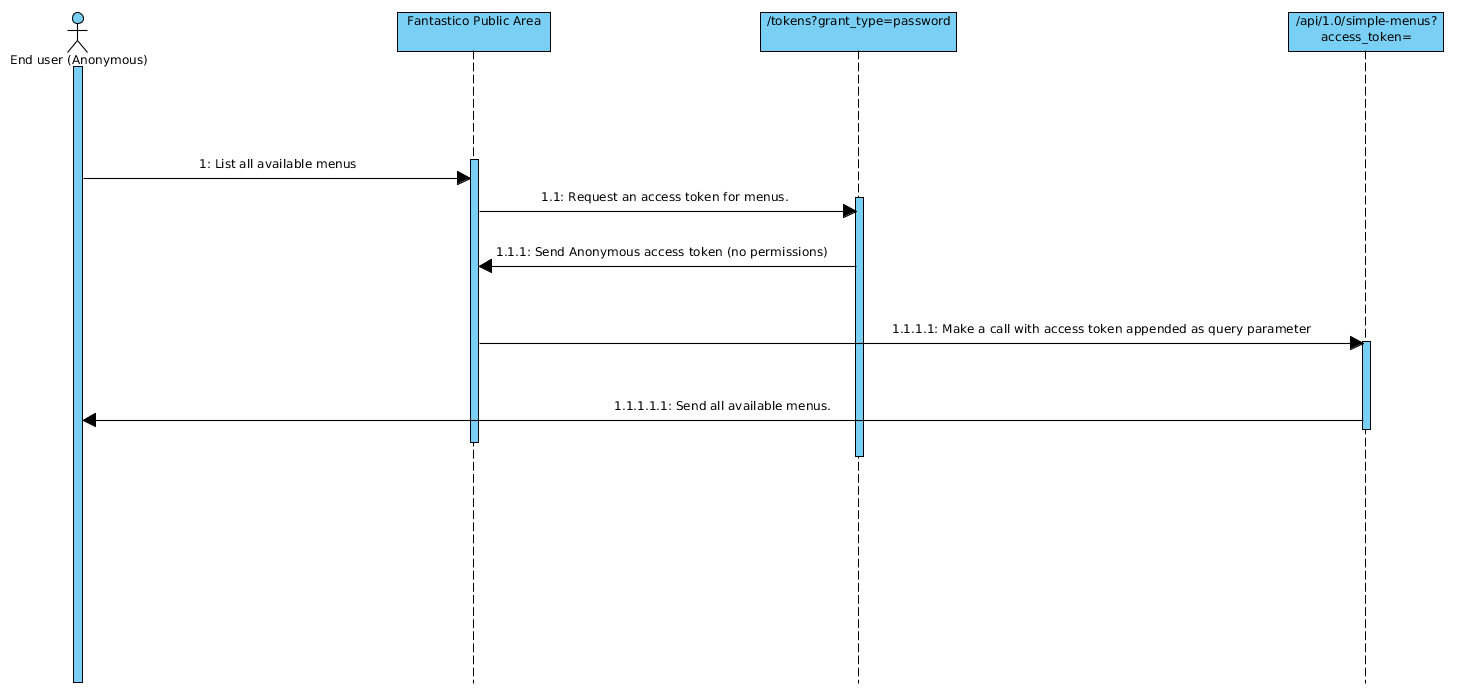
\includegraphics{simple_menu_read.png}

As you can see in the above example read access is pretty straightforward because the read endpoint (route) does not require
authorization (specific scopes).


\paragraph{Managing menus.}
\label{features/oauth2/simple_api_example:oauth-create-new-menu}\label{features/oauth2/simple_api_example:managing-menus}
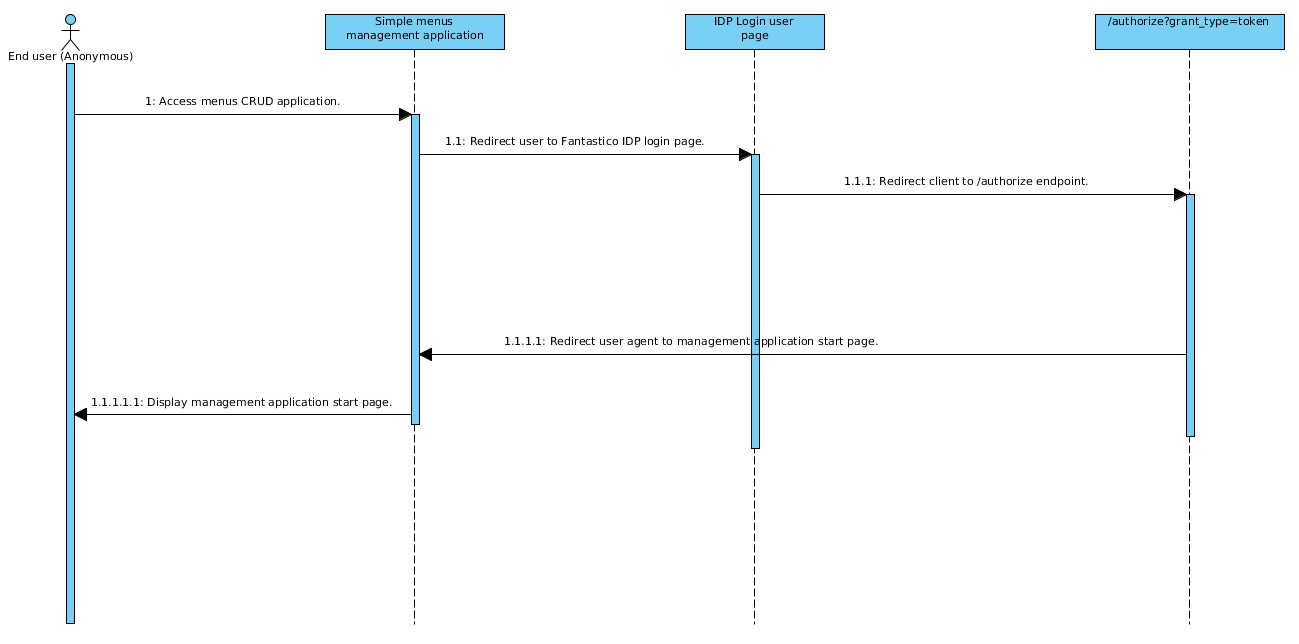
\includegraphics{simple_menu_create.png}

The above diagram assumes an application exists for managing \textbf{menus}. This application (extension) consist of a set of frontend
controllers which renders only markup and a set of \textbf{REST APIs} described above. The above diagram assumes \textbf{End user} uses an
user agent capable of supporting HTTP protocol. Below you can find the http calls made:
\begin{enumerate}
\item {} 
Unauthenticated user requests:

\begin{Verbatim}[commandchars=\\\{\}]
GET - /authorize?response\_type=token\&client\_id=sample-menus\&state=xyz\&error\_format=hash\&redirect\_uri=/simple-menus/ui/index\&scopes=simple\_menus.create\%20simple\_menus.update\%20simple\_menus.delete
\end{Verbatim}

\item {} 
Fantastico /authorize endpoint detects that user is not authenticated and redirects the user agent to login screen.

\item {} 
If authentication is successful user agent is redirected back to /authorize.

\item {} 
At this point an access token is generated and user agent is redirected back to simple menus ui index page with an access token in hash.

\item {} 
Menus management application start page stores the access token into the application space (session storage might be used for this).
It is recommended to validate received state in order to ensure it corresponds to the initial request state. Application must decide
how to generate state and keep it consistent before request and response.

\end{enumerate}

This is it. Using the access token, end user can easily access desired functionality. Moreover, using the access token,
menus management application can easily invoke apis.


\subsubsection{OAUTH2 Fantastico Tokens}
\label{features/oauth2/tokens_format:oauth2-fantastico-tokens}\label{features/oauth2/tokens_format::doc}
In Fantastico framework there are currently two type of supported tokens:
\begin{itemize}
\item {} 
Authenticated user token.
\begin{quote}

An opaque value used to prove the requester (end user) is indeed authenticated. This token is set once by the Fantastico IDP
login page and lives a long time (couple of weeks). The structure of this opaque value as seen on server side is presented
below:
\begin{quote}

\begin{Verbatim}[commandchars=\\\{\}]
\PYG{p}{\PYGZob{}}\PYG{l+s+s2}{\PYGZdq{}client\PYGZus{}id\PYGZdq{}}\PYG{o}{:} \PYG{l+s+s2}{\PYGZdq{}fantastico\PYGZhy{}idp\PYGZdq{}}\PYG{p}{,}
 \PYG{l+s+s2}{\PYGZdq{}type\PYGZdq{}}\PYG{o}{:} \PYG{l+s+s2}{\PYGZdq{}login\PYGZdq{}}\PYG{p}{,}
 \PYG{l+s+s2}{\PYGZdq{}encrypted\PYGZdq{}}\PYG{o}{:} \PYG{p}{\PYGZob{}}
    \PYG{l+s+s2}{\PYGZdq{}client\PYGZus{}id\PYGZdq{}}\PYG{o}{:} \PYG{l+s+s2}{\PYGZdq{}fantastico\PYGZhy{}idp\PYGZdq{}}\PYG{p}{,}
    \PYG{l+s+s2}{\PYGZdq{}type\PYGZdq{}}\PYG{o}{:} \PYG{l+s+s2}{\PYGZdq{}login\PYGZdq{}}\PYG{p}{,}
    \PYG{l+s+s2}{\PYGZdq{}user\PYGZus{}id\PYGZdq{}}\PYG{o}{:} \PYG{l+m+mi}{1}\PYG{p}{,}
    \PYG{l+s+s2}{\PYGZdq{}creation\PYGZus{}time\PYGZdq{}}\PYG{o}{:} \PYG{l+s+s2}{\PYGZdq{}1380137651\PYGZdq{}}\PYG{p}{,}
    \PYG{l+s+s2}{\PYGZdq{}expiration\PYGZus{}time\PYGZdq{}}\PYG{o}{:} \PYG{l+s+s2}{\PYGZdq{}1380163800\PYGZdq{}}\PYG{p}{,}
 \PYG{p}{\PYGZcb{}}
\PYG{p}{\PYGZcb{}}
\end{Verbatim}
\end{quote}
\end{quote}

\item {} 
Access token
\begin{quote}

An opaque value used to allow applications to access resource owner resources (images, documents, menus, etc). Below you can
find the access token structure, as seen on server side:
\begin{quote}

\begin{Verbatim}[commandchars=\\\{\}]
\PYG{p}{\PYGZob{}}\PYG{l+s+s2}{\PYGZdq{}client\PYGZus{}id\PYGZdq{}}\PYG{o}{:} \PYG{l+s+s2}{\PYGZdq{}simple\PYGZhy{}menus\PYGZdq{}}\PYG{p}{,}
 \PYG{l+s+s2}{\PYGZdq{}type\PYGZdq{}}\PYG{o}{:} \PYG{l+s+s2}{\PYGZdq{}access\PYGZdq{}}\PYG{p}{,}
 \PYG{l+s+s2}{\PYGZdq{}encrypted\PYGZdq{}}\PYG{o}{:} \PYG{p}{\PYGZob{}}
   \PYG{l+s+s2}{\PYGZdq{}client\PYGZus{}id\PYGZdq{}}\PYG{o}{:} \PYG{l+s+s2}{\PYGZdq{}simple\PYGZhy{}menus\PYGZdq{}}\PYG{p}{,}
   \PYG{l+s+s2}{\PYGZdq{}type\PYGZdq{}}\PYG{o}{:} \PYG{l+s+s2}{\PYGZdq{}access\PYGZdq{}}\PYG{p}{,}
   \PYG{l+s+s2}{\PYGZdq{}user\PYGZus{}id\PYGZdq{}}\PYG{o}{:} \PYG{l+m+mi}{1}\PYG{p}{,}
   \PYG{l+s+s2}{\PYGZdq{}scopes\PYGZdq{}}\PYG{o}{:} \PYG{p}{[}\PYG{l+s+s2}{\PYGZdq{}simple\PYGZus{}menus.create\PYGZdq{}}\PYG{p}{,} \PYG{l+s+s2}{\PYGZdq{}simple\PYGZus{}menus.update\PYGZdq{}}\PYG{p}{,} \PYG{l+s+s2}{\PYGZdq{}simple\PYGZus{}menus.delete\PYGZdq{}}\PYG{p}{]}\PYG{p}{,}
   \PYG{l+s+s2}{\PYGZdq{}creation\PYGZus{}time\PYGZdq{}}\PYG{o}{:} \PYG{l+s+s2}{\PYGZdq{}1380137651\PYGZdq{}}\PYG{p}{,}
   \PYG{l+s+s2}{\PYGZdq{}expiration\PYGZus{}time\PYGZdq{}}\PYG{o}{:} \PYG{l+s+s2}{\PYGZdq{}1380163800\PYGZdq{}}
 \PYG{p}{\PYGZcb{}}
\PYG{p}{\PYGZcb{}}
\end{Verbatim}
\end{quote}
\end{quote}

\end{itemize}

All supported tokens are symmetrical encrypted by Fantastico on server side and though become opaque for the user agent. Currently,
AES-256 is used for encryption.


\subsubsection{OAUTH2 Fantastico Error Responses}
\label{features/oauth2/error_responses::doc}\label{features/oauth2/error_responses:oauth2-fantastico-error-responses}
In this section you can find possible error responses retrieved by \textbf{Fantastico} OAUTH2 endpoints.


\paragraph{/authorize}
\label{features/oauth2/error_responses:authorize}
Below attributes are appended as query parameters or sent as json object to the client application in case of an exception:
\begin{itemize}
\item {} 
error
\begin{itemize}
\item {} 
\textbf{400 Bad request}
\begin{itemize}
\item {} 
invalid\_request
\begin{quote}

The request is missing a required parameter, includes an invalid parameter value, includes a parameter more than once,
or is otherwise malformed.
\end{quote}

\item {} 
unsupported\_response\_type
\begin{quote}

The authorization server does not support obtaining an authorization / access token code using this method.
\end{quote}

\item {} 
invalid\_scope
\begin{quote}

The requested scope is invalid, unknown, or malformed.
\end{quote}

\end{itemize}

\item {} 
\textbf{401 Unauthorized}
\begin{itemize}
\item {} 
unauthorized\_client
\begin{quote}

The client is not authorized to request an authorization code / access token using this method.
\end{quote}

\end{itemize}

\item {} 
\textbf{403 Forbidden}
\begin{itemize}
\item {} 
access\_denied
\begin{quote}

The resource owner or authorization server denied the request.
\end{quote}

\end{itemize}

\end{itemize}

\item {} 
error\_description
\begin{quote}

Human-readable ASCII {[}USASCII{]} text providing additional information, used to assist the client developer in
understanding the error that occurred.
\end{quote}

\item {} 
error\_uri
\begin{quote}

A URI identifying a human-readable web page with information about the error, used to provide the client developer
with additional information about the error.
\end{quote}

\end{itemize}


\subsubsection{OAUTH2 Fantastico App registration}
\label{features/oauth2/app_registration::doc}\label{features/oauth2/app_registration:oauth2-fantastico-app-registration}
In order to be able to develop secure applications on Fantastico, you must first register them in order to be able to obtain
access tokens. Before moving forward to see supported ways to register applications into a project it is important to understand
the data structure presented below:

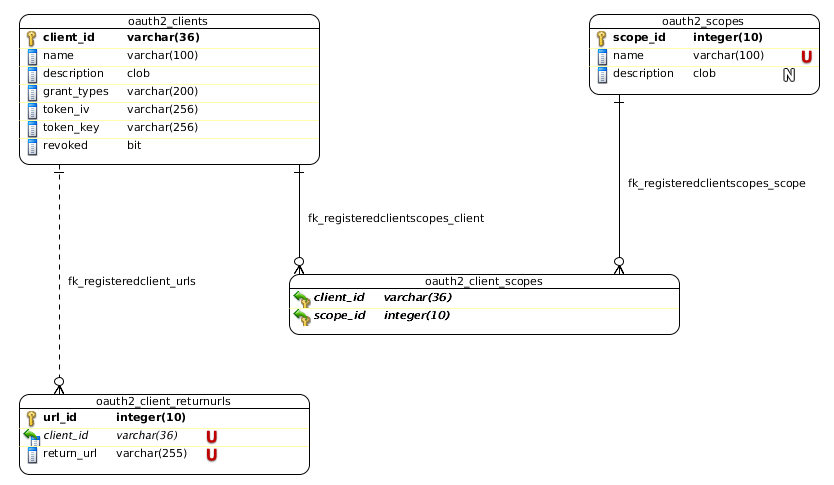
\includegraphics{clients_storage.png}

Summarizing the diagram above, a client is described by:
\begin{itemize}
\item {} 
\textbf{client\_id}
\begin{quote}

A global unique identifier for the application within a Fantastico project.
\end{quote}

\item {} 
\textbf{name}
\begin{quote}

A friendly name which accurately describes what is the purpose of this application.
\end{quote}

\item {} 
\textbf{description}
\begin{quote}

(Optional) A human readable text detailing the benefits of this application.
\end{quote}

\item {} 
\textbf{grant\_types}
\begin{quote}

A comma separated list of values describing what OAuth 2 grant types this client can use in order to obtain an access token.
\end{quote}

\item {} 
\textbf{scopes}
\begin{quote}

This is a list of scopes this application is authorized to use.
\end{quote}

\item {} 
\textbf{token\_iv}
\begin{quote}

A 128 bits initialization vector specific to this client used to initialize AES algorithm.
\end{quote}

\item {} 
\textbf{token\_key}
\begin{quote}

A (128 / 192 / 256) bits key used for AES algorithm.
\end{quote}

\item {} 
\textbf{return\_urls}
\begin{quote}

A list of return urls which Fantastico OAauth 2 authorize is allowed to redirect user agent of end user.
\end{quote}

\end{itemize}


\paragraph{App registration extension}
\label{features/oauth2/app_registration:app-registration-extension}
This is a Fantastico extension used to allow new apps registration into an existing project. In order to enable this extension
in your project follow the steps below:
\begin{enumerate}
\item {} 
Activate the extension.

\begin{Verbatim}[commandchars=\\\{\}]
fsdk activate\PYGZhy{}extenstion \PYGZhy{}\PYGZhy{}name oauth2\PYGZhy{}registration \PYGZhy{}\PYGZhy{}comp\PYGZhy{}root \PYGZlt{}your components root folder\PYGZgt{}
\end{Verbatim}

\item {} 
Synchronize database.

\begin{Verbatim}[commandchars=\\\{\}]
fsdk syncdb \PYGZhy{}\PYGZhy{}db\PYGZhy{}command /usr/bin/mysql \PYGZhy{}\PYGZhy{}comp\PYGZhy{}root \PYGZlt{}your components root folder\PYGZgt{}
\end{Verbatim}

\item {} 
Start your development server.

\item {} 
Access \href{http://localhost:12000/oauth/oauth2-registration/index}{http://localhost:12000/oauth/oauth2-registration/index}

\end{enumerate}

You can find more information about this extension on \code{/features/components/oauth2/app\_registration/index}.


\paragraph{Manual registration}
\label{features/oauth2/app_registration:manual-registration}
Even if it's really easy to use the frontend for registering applications, when you will migrate your project to production
you will definitely want to automatically register the applications using a script. The easiest way is to dump \textbf{RegisteredClients}
table content into a \textbf{create\_data.sql} script placed under your main component.

By doing this, next time you sync your database in production using {\hyperref[features/sdk::doc]{\emph{SDK}}} it will preregister all necessary
applications. Please make sure you do not include \textbf{oauth2-registration} client id. This is automatically added by the extension.


\subsubsection{Controllers security}
\label{features/oauth2/controllers_security:controllers-security}\label{features/oauth2/controllers_security::doc}

\paragraph{Regular controllers security}
\label{features/oauth2/controllers_security:regular-controllers-security}
In general, you will want to secure your controllers ({\hyperref[how_to/mvc_how_to::doc]{\emph{MVC How to}}}) using OAuth2. In addition, for some controllers
(e.g UI Controllers) you will want to tell Fantastico to redirect automatically to login screen rather than returning an
\textbf{401 Unauthorized} error. Below you can find a very simple example of a ui controller which automatically redirects user to
login screen in order to obtain access:

\begin{Verbatim}[commandchars=\\\{\}]
\PYG{n+nd}{@ControllerProvider}\PYG{p}{(}\PYG{p}{)}
\PYG{k}{class} \PYG{n+nc}{SecuredController}\PYG{p}{(}\PYG{n}{BaseController}\PYG{p}{)}\PYG{p}{:}
    \PYG{n+nd}{@RequiredScopes}\PYG{p}{(}\PYG{n}{scopes}\PYG{o}{=}\PYG{p}{[}\PYG{l+s}{\PYGZdq{}}\PYG{l+s}{greet.verbose}\PYG{l+s}{\PYGZdq{}}\PYG{p}{,} \PYG{l+s}{\PYGZdq{}}\PYG{l+s}{greet.read}\PYG{l+s}{\PYGZdq{}}\PYG{p}{]}\PYG{p}{)}
    \PYG{n+nd}{@Controller}\PYG{p}{(}\PYG{n}{url}\PYG{o}{=}\PYG{l+s}{\PYGZdq{}}\PYG{l+s}{/secured\PYGZhy{}controller/ui/index}\PYG{l+s}{\PYGZdq{}}\PYG{p}{)}
    \PYG{k}{def} \PYG{n+nf}{say\PYGZus{}hello}\PYG{p}{(}\PYG{n+nb+bp}{self}\PYG{p}{,} \PYG{n}{request}\PYG{p}{)}\PYG{p}{:}
        \PYG{k}{return} \PYG{l+s}{\PYGZdq{}}\PYG{l+s}{\PYGZlt{}html\PYGZgt{}\PYGZlt{}body\PYGZgt{}\PYGZlt{}h1\PYGZgt{}Hello world\PYGZlt{}/body\PYGZgt{}\PYGZlt{}/html\PYGZgt{}}\PYG{l+s}{\PYGZdq{}}
\end{Verbatim}

The order in which decorators are chained is extremely important because \textbf{RequiredScopes} append an attribute to security context
while \textbf{Controller} triggers security context validation.


\paragraph{ROA OAUTH2 Security}
\label{features/oauth2/controllers_security:roa-oauth2-security}
ROA ({\hyperref[features/roa::doc]{\emph{ROA (Resource Oriented Architecture)}}}) resource can be easily secured using OAuth2 as shown below:

\begin{Verbatim}[commandchars=\\\{\}]
\PYG{n+nd}{@Resource}\PYG{p}{(}\PYG{n}{name}\PYG{o}{=}\PYG{l+s}{\PYGZdq{}}\PYG{l+s}{app\PYGZhy{}setting}\PYG{l+s}{\PYGZdq{}}\PYG{p}{,} \PYG{n}{url}\PYG{o}{=}\PYG{l+s}{\PYGZdq{}}\PYG{l+s}{/app\PYGZhy{}settings}\PYG{l+s}{\PYGZdq{}}\PYG{p}{,} \PYG{n}{version}\PYG{o}{=}\PYG{l+m+mf}{1.0}\PYG{p}{)}
\PYG{n+nd}{@RequiredScopes}\PYG{p}{(}\PYG{n}{create}\PYG{o}{=}\PYG{p}{[}\PYG{l+s}{\PYGZdq{}}\PYG{l+s}{app\PYGZus{}setting.create}\PYG{l+s}{\PYGZdq{}}\PYG{p}{]}\PYG{p}{,}
                \PYG{n}{read}\PYG{o}{=}\PYG{p}{[}\PYG{l+s}{\PYGZdq{}}\PYG{l+s}{app\PYGZus{}setting.read}\PYG{l+s}{\PYGZdq{}}\PYG{p}{]}\PYG{p}{,}
                \PYG{n}{update}\PYG{o}{=}\PYG{p}{[}\PYG{l+s}{\PYGZdq{}}\PYG{l+s}{app\PYGZus{}setting.update}\PYG{l+s}{\PYGZdq{}}\PYG{p}{]}\PYG{p}{,}
                \PYG{n}{delete}\PYG{o}{=}\PYG{p}{[}\PYG{l+s}{\PYGZdq{}}\PYG{l+s}{app\PYGZus{}setting.delete}\PYG{l+s}{\PYGZdq{}}\PYG{p}{]}\PYG{p}{\PYGZcb{}}\PYG{p}{)}
\PYG{k}{class} \PYG{n+nc}{AppSetting}\PYG{p}{(}\PYG{n}{BASEMODEL}\PYG{p}{)}\PYG{p}{:}
    \PYG{n+nb}{id} \PYG{o}{=} \PYG{n}{Column}\PYG{p}{(}\PYG{l+s}{\PYGZdq{}}\PYG{l+s}{id}\PYG{l+s}{\PYGZdq{}}\PYG{p}{,} \PYG{n}{Integer}\PYG{p}{,} \PYG{n}{primary\PYGZus{}key}\PYG{o}{=}\PYG{n+nb+bp}{True}\PYG{p}{,} \PYG{n}{autoincrement}\PYG{o}{=}\PYG{n+nb+bp}{True}\PYG{p}{)}
    \PYG{n}{name} \PYG{o}{=} \PYG{n}{Column}\PYG{p}{(}\PYG{l+s}{\PYGZdq{}}\PYG{l+s}{name}\PYG{l+s}{\PYGZdq{}}\PYG{p}{,} \PYG{n}{String}\PYG{p}{(}\PYG{l+m+mi}{50}\PYG{p}{)}\PYG{p}{,} \PYG{n}{unique}\PYG{o}{=}\PYG{n+nb+bp}{True}\PYG{p}{,} \PYG{n}{nullable}\PYG{o}{=}\PYG{n+nb+bp}{False}\PYG{p}{)}
    \PYG{n}{value} \PYG{o}{=} \PYG{n}{Column}\PYG{p}{(}\PYG{l+s}{\PYGZdq{}}\PYG{l+s}{value}\PYG{l+s}{\PYGZdq{}}\PYG{p}{,} \PYG{n}{Text}\PYG{p}{,} \PYG{n}{nullable}\PYG{o}{=}\PYG{n+nb+bp}{False}\PYG{p}{)}

    \PYG{k}{def} \PYG{n+nf}{\PYGZus{}\PYGZus{}init\PYGZus{}\PYGZus{}}\PYG{p}{(}\PYG{n+nb+bp}{self}\PYG{p}{,} \PYG{n}{name}\PYG{p}{,} \PYG{n}{value}\PYG{p}{)}\PYG{p}{:}
        \PYG{n+nb+bp}{self}\PYG{o}{.}\PYG{n}{name} \PYG{o}{=} \PYG{n}{name}
        \PYG{n+nb+bp}{self}\PYG{o}{.}\PYG{n}{value} \PYG{o}{=} \PYG{n}{value}
\end{Verbatim}

This is an extremely convenient way to secure a resource. In addition, each argument from \textbf{@Resource} constructor is optional.
For instance, if read is not given any scope then everyone can read \textbf{AppSetting} resources.

Fantastico will autodiscover endpoints / resources which require scopes and preauthorize every call to them.


\subsubsection{OAUTH2 Fantastico IDP}
\label{features/oauth2/idp:oauth2-fantastico-idp}\label{features/oauth2/idp::doc}
Fantastico provides a default Identity provider which provides required APIs for managing users. As other Fantastico
extensions APIs, idp APIs are secured with OAUTH2 tokens. In order to activate IDP extension for \textbf{Fantastico} follow
{\hyperref[features/components/oauth2/oauth2_idp/index::doc]{\emph{OAuth2 Identity Provider}}}.


\paragraph{APIs}
\label{features/oauth2/idp:apis}
\begin{tabulary}{\linewidth}{|L|L|L|L|L|}
\hline

\textbf{URI}
 & 
\textbf{Verb}
 & 
\textbf{Required scopes}
 & 
\textbf{Description}
 & 
\textbf{Headers}
\\\hline

\textbf{/api/latest/oauth-idp-profile}
 & 
GET
 & 
user.profile.read
 & 
Retrieves information about authenticated user.
 & 
Authorization: Bearer \textless{}oauth2\_token\textgreater{}
\\\hline

\textbf{/api/latest/oauth-idp-profile}
 & 
POST
 &  & 
Creates a new user profile.
 & \\\hline

\textbf{/api/latest/oauth-idp-profile}
 & 
PUT
 & 
user.profile.update
 & 
Updates an existing user profile.
 & 
Authorization: Bearer \textless{}oauth2\_token\textgreater{}
\\\hline

\textbf{/api/latest/oauth-idp-profile}
 & 
DELETE
 & 
user.profile.delete
 & 
Updates an existing user profile.
 & 
Authorization: Bearer \textless{}oauth2\_token\textgreater{}
\\\hline

\textbf{/api/latest/oauth-idp-person/:person\_id}
 & 
PUT
 & 
user.profile.update
 & 
Updates existing person details .
 & 
Authorization: Bearer \textless{}oauth2\_token\textgreater{}
\\\hline

\textbf{/oauth/idp/ui/login?redirect\_uri=/test-url}
 & 
GET
 &  & 
Returns the markup for login screen.
 & \\\hline

\textbf{/oauth/idp/login?redirect\_uri=/test-url}
 & 
POST
 &  & 
Authenticate the user, generates a token and passes it to redirect uri.
 & \\\hline

\textbf{/oauth/idp/ui/cb}
 & 
GET
 &  & 
A very simple callback which extracts the access token received and prints it on screen.
 & \\\hline
\end{tabulary}



\paragraph{User profile data}
\label{features/oauth2/idp:user-profile-data}
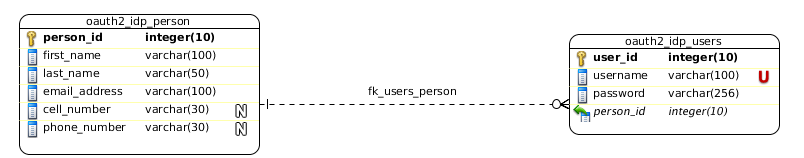
\includegraphics{idp_profiles.png}


\paragraph{Login frontend}
\label{features/oauth2/idp:login-frontend}
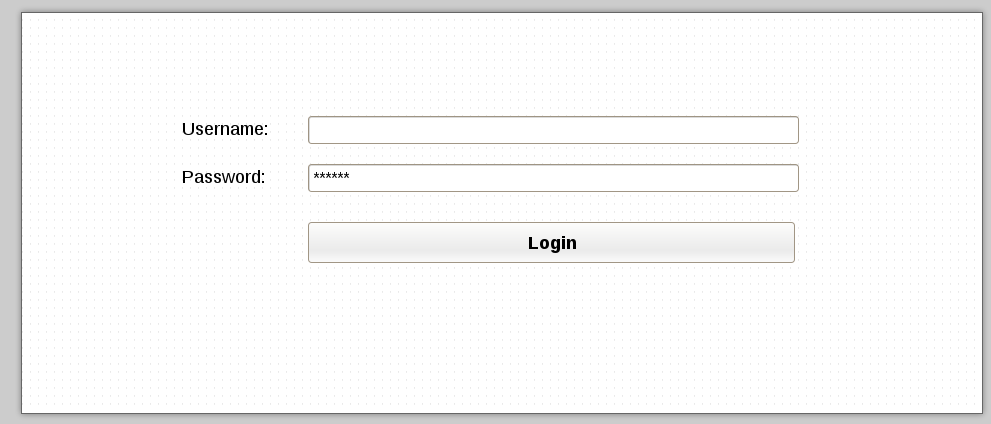
\includegraphics{idp_login.png}

Developers can easily customize the login screen by providing a template which must be applied to login screen. A typical custom
login template is presented below:

\begin{Verbatim}[commandchars=\\\{\}]
\PYGZob{}\PYGZpc{} extends \PYGZdq{}login.html\PYGZdq{} \PYGZpc{}\PYGZcb{}

\PYGZob{}\PYGZpc{} block head \PYGZpc{}\PYGZcb{}
    \PYG{n+nt}{\PYGZlt{}title}\PYG{n+nt}{\PYGZgt{}}Fantastico IDP default login\PYG{n+nt}{\PYGZlt{}/title\PYGZgt{}}

    \PYG{c}{\PYGZlt{}!\PYGZhy{}\PYGZhy{}}\PYG{c}{ Latest compiled and minified CSS }\PYG{c}{\PYGZhy{}\PYGZhy{}\PYGZgt{}}
    \PYG{n+nt}{\PYGZlt{}link} \PYG{n+na}{rel=}\PYG{l+s}{\PYGZdq{}stylesheet\PYGZdq{}} \PYG{n+na}{href=}\PYG{l+s}{\PYGZdq{}//netdna.bootstrapcdn.com/bootstrap/3.0.3/css/bootstrap.min.css\PYGZdq{}}\PYG{n+nt}{\PYGZgt{}}
    \PYG{n+nt}{\PYGZlt{}link} \PYG{n+na}{rel=}\PYG{l+s}{\PYGZdq{}stylesheet\PYGZdq{}} \PYG{n+na}{href=}\PYG{l+s}{\PYGZdq{}//netdna.bootstrapcdn.com/bootstrap/3.0.3/css/bootstrap\PYGZhy{}theme.min.css\PYGZdq{}}\PYG{n+nt}{\PYGZgt{}}

    \PYG{n+nt}{\PYGZlt{}script }\PYG{n+na}{src=}\PYG{l+s}{\PYGZdq{}//code.jquery.com/jquery\PYGZhy{}2.0.3.min.js\PYGZdq{}}\PYG{n+nt}{\PYGZgt{}}\PYG{n+nt}{\PYGZlt{}/script\PYGZgt{}}
    \PYG{n+nt}{\PYGZlt{}script }\PYG{n+na}{src=}\PYG{l+s}{\PYGZdq{}//netdna.bootstrapcdn.com/bootstrap/3.0.3/js/bootstrap.min.js\PYGZdq{}}\PYG{n+nt}{\PYGZgt{}}\PYG{n+nt}{\PYGZlt{}/script\PYGZgt{}}
\PYGZob{}\PYGZpc{} endblock \PYGZpc{}\PYGZcb{}

\PYGZob{}\PYGZpc{} block body\PYGZus{}header \PYGZpc{}\PYGZcb{}
\PYG{n+nt}{\PYGZlt{}div} \PYG{n+na}{class=}\PYG{l+s}{\PYGZdq{}row\PYGZdq{}} \PYG{n+na}{align=}\PYG{l+s}{\PYGZdq{}center\PYGZdq{}}\PYG{n+nt}{\PYGZgt{}}
    \PYG{n+nt}{\PYGZlt{}div} \PYG{n+na}{class=}\PYG{l+s}{\PYGZdq{}col\PYGZhy{}md\PYGZhy{}4\PYGZdq{}}\PYG{n+nt}{\PYGZgt{}}
        \PYG{n+nt}{\PYGZlt{}div} \PYG{n+na}{class=}\PYG{l+s}{\PYGZdq{}panel panel\PYGZhy{}default\PYGZdq{}}\PYG{n+nt}{\PYGZgt{}}
            \PYG{n+nt}{\PYGZlt{}div} \PYG{n+na}{class=}\PYG{l+s}{\PYGZdq{}panel\PYGZhy{}heading\PYGZdq{}}\PYG{n+nt}{\PYGZgt{}}
                \PYGZob{}\PYGZpc{} block panel\PYGZus{}header \PYGZpc{}\PYGZcb{}
                \PYG{n+nt}{\PYGZlt{}h1}\PYG{n+nt}{\PYGZgt{}}Login to fantastico\PYG{n+nt}{\PYGZlt{}/h1\PYGZgt{}}
                \PYGZob{}\PYGZpc{} endblock \PYGZpc{}\PYGZcb{}
            \PYG{n+nt}{\PYGZlt{}/div\PYGZgt{}}
\PYGZob{}\PYGZpc{} endblock \PYGZpc{}\PYGZcb{}

\PYGZob{}\PYGZpc{} block body\PYGZus{}footer \PYGZpc{}\PYGZcb{}
            \PYG{n+nt}{\PYGZlt{}div} \PYG{n+na}{class=}\PYG{l+s}{\PYGZdq{}panel\PYGZhy{}footer\PYGZdq{}}\PYG{n+nt}{\PYGZgt{}}
                \PYG{n+nt}{\PYGZlt{}h4}\PYG{n+nt}{\PYGZgt{}}Created by Radu Viorel Cosnita\PYG{n+nt}{\PYGZlt{}/h4\PYGZgt{}}
            \PYG{n+nt}{\PYGZlt{}/div\PYGZgt{}}
        \PYG{n+nt}{\PYGZlt{}/div\PYGZgt{}}
    \PYG{n+nt}{\PYGZlt{}/div\PYGZgt{}}
\PYG{n+nt}{\PYGZlt{}/div\PYGZgt{}}
\PYGZob{}\PYGZpc{} endblock \PYGZpc{}\PYGZcb{}
\end{Verbatim}

You can find documentation on how to configure custom login template on {\hyperref[get_started/settings::doc]{\emph{Fantastico settings}}}.


\subparagraph{Administrator account}
\label{features/oauth2/idp:administrator-account}
When you first activate the extension and you syncdb an administrator account is created:

\begin{Verbatim}[commandchars=\\\{\}]
\PYG{n+nv}{username} \PYG{o}{=} \PYG{l+s+s2}{\PYGZdq{}admin@fantastico.com\PYGZdq{}}
\PYG{n+nv}{password} \PYG{o}{=} \PYG{l+s+s2}{\PYGZdq{}1234567890\PYGZdq{}}
\end{Verbatim}

This account can be used to access various applications provided by various Fantastico extensions.


\subparagraph{Users and persons}
\label{features/oauth2/idp:users-and-persons}
At the current moment a person can only have one user associated. Person details must be retrieved using oauth-idp-profile complex
representation (see: {\hyperref[features/roa::doc]{\emph{ROA (Resource Oriented Architecture)}}}). Moreover, when a new user is created a new person is created automatically and
assigned to that user. Initially created person has some default values in order to allow very smooth account creation in various
applications.


\paragraph{Default oauth callback}
\label{features/oauth2/idp:default-oauth-callback}
By default, the oauth idp also provides a callback page which displays received hash parameters. In order to allow reusage of this callback
in mobile apps this callback page sends \textbf{fantastico.oauth.cb.message} message to it's parent frame with the following body:

\begin{Verbatim}[commandchars=\\\{\}]
\PYG{p}{\PYGZob{}}
   \PYG{l+s+s2}{\PYGZdq{}messageType\PYGZdq{}}\PYG{o}{:} \PYG{l+s+s2}{\PYGZdq{}fantastico.oauth.cb.message\PYGZdq{}}\PYG{p}{,}
   \PYG{l+s+s2}{\PYGZdq{}url\PYGZdq{}}\PYG{o}{:} \PYG{l+s+s2}{\PYGZdq{}\PYGZlt{}current url include hash fragment\PYGZgt{}\PYGZdq{}}\PYG{p}{,}
   \PYG{l+s+s2}{\PYGZdq{}access\PYGZus{}token\PYGZdq{}}\PYG{o}{:} \PYG{l+s+s2}{\PYGZdq{}\PYGZlt{}currently received access token\PYGZgt{}\PYGZdq{}}\PYG{p}{,}
   \PYG{l+s+s2}{\PYGZdq{}expires\PYGZus{}in\PYGZdq{}}\PYG{o}{:} \PYG{l+s+s2}{\PYGZdq{}\PYGZlt{}the number of minutes in which access token will expire\PYGZgt{}\PYGZdq{}}
\PYG{p}{\PYGZcb{}}
\end{Verbatim}

In case of an error the same message is sent with error attributes received in hash fragment.


\paragraph{Technical summary}
\label{features/oauth2/idp:technical-summary}

\subparagraph{Password storage}
\label{features/oauth2/idp:password-storage}
It is recommend that each identity provider holds hashes of passwords instead of plain text passwords. Foreasily development of
new Identity Providers, Fantastico provides a contract for easily hashing passwords.
\index{PasswordsHasher (class in fantastico.oauth2.passwords\_hasher)}

\begin{fulllineitems}
\phantomsection\label{features/oauth2/idp:fantastico.oauth2.passwords_hasher.PasswordsHasher}\pysigline{\strong{class }\code{fantastico.oauth2.passwords\_hasher.}\bfcode{PasswordsHasher}}
This class provides an abstract contract for password hasher. A password hasher is an algorithm that generates a strong
hash starting from a plain text string.
\index{hash\_password() (fantastico.oauth2.passwords\_hasher.PasswordsHasher method)}

\begin{fulllineitems}
\phantomsection\label{features/oauth2/idp:fantastico.oauth2.passwords_hasher.PasswordsHasher.hash_password}\pysiglinewithargsret{\bfcode{hash\_password}}{\emph{plain\_passwd}, \emph{hash\_ctx=None}}{}
This method must be overriden in order to provide concrete hashing algorithm.
\begin{quote}\begin{description}
\item[{Parameters}] \leavevmode\begin{itemize}
\item {} 
\textbf{plain\_passwd} (\emph{str}) -- The plain password for which we want to obtain a strong hash.

\item {} 
\textbf{hash\_ctx} (\code{fantastico.utils.dictionary\_object.DictionaryObject}) -- An optional hashing context which contains additional attributes required by hashing algorithm. E.g: sha512 with salt.

\end{itemize}

\item[{Returns}] \leavevmode
The strong hash generated.

\item[{Return type}] \leavevmode
str

\end{description}\end{quote}

\end{fulllineitems}


\end{fulllineitems}

\index{Sha512SaltPasswordsHasher (class in fantastico.oauth2.sha512salt\_passwords\_hasher)}

\begin{fulllineitems}
\phantomsection\label{features/oauth2/idp:fantastico.oauth2.sha512salt_passwords_hasher.Sha512SaltPasswordsHasher}\pysigline{\strong{class }\code{fantastico.oauth2.sha512salt\_passwords\_hasher.}\bfcode{Sha512SaltPasswordsHasher}}
This class provides the sha512salt implementation for password hashing. In addition, the result is encoded using base64.
In order to use this hasher try the code snippet below:

\begin{Verbatim}[commandchars=\\\{\}]
\PYG{n}{sha512\PYGZus{}hasher} \PYG{o}{=} \PYG{n}{PasswordsHasherFactory}\PYG{p}{(}\PYG{p}{)}\PYG{o}{.}\PYG{n}{get\PYGZus{}hasher}\PYG{p}{(}\PYG{n}{PasswordsHasherFactory}\PYG{o}{.}\PYG{n}{SHA512\PYGZus{}SALT}\PYG{p}{)}
\PYG{n}{hashed\PYGZus{}passwd} \PYG{o}{=} \PYG{n}{sha512\PYGZus{}hasher}\PYG{o}{.}\PYG{n}{hash\PYGZus{}password}\PYG{p}{(}\PYG{l+s}{\PYGZdq{}}\PYG{l+s}{abcd}\PYG{l+s}{\PYGZdq{}}\PYG{p}{,} \PYG{n}{DictionaryObject}\PYG{p}{(}\PYG{p}{\PYGZob{}}\PYG{l+s}{\PYGZdq{}}\PYG{l+s}{salt}\PYG{l+s}{\PYGZdq{}}\PYG{p}{:} \PYG{l+m+mi}{123}\PYG{p}{\PYGZcb{}}\PYG{p}{)}\PYG{p}{)}
\end{Verbatim}
\index{hash\_password() (fantastico.oauth2.sha512salt\_passwords\_hasher.Sha512SaltPasswordsHasher method)}

\begin{fulllineitems}
\phantomsection\label{features/oauth2/idp:fantastico.oauth2.sha512salt_passwords_hasher.Sha512SaltPasswordsHasher.hash_password}\pysiglinewithargsret{\bfcode{hash\_password}}{\emph{plain\_passwd}, \emph{hash\_ctx=None}}{}
This method provides the sha512 with salt algorithm for a given plain password. In addition, the hash is base64
encoded.

\end{fulllineitems}


\end{fulllineitems}

\index{PasswordsHasherFactory (class in fantastico.oauth2.passwords\_hasher\_factory)}

\begin{fulllineitems}
\phantomsection\label{features/oauth2/idp:fantastico.oauth2.passwords_hasher_factory.PasswordsHasherFactory}\pysigline{\strong{class }\code{fantastico.oauth2.passwords\_hasher\_factory.}\bfcode{PasswordsHasherFactory}}
This class provides a factory used to obtain concrete password hasher providers. At the moment, the following
hashers are supported:
\begin{itemize}
\item {} 
SHA512\_SALT

\end{itemize}
\index{get\_hasher() (fantastico.oauth2.passwords\_hasher\_factory.PasswordsHasherFactory method)}

\begin{fulllineitems}
\phantomsection\label{features/oauth2/idp:fantastico.oauth2.passwords_hasher_factory.PasswordsHasherFactory.get_hasher}\pysiglinewithargsret{\bfcode{get\_hasher}}{\emph{hash\_alg}}{}
This method obtains a concrete passwords hasher provider based on the requested hash algorithm. See the constants
defined in this factory in order to find out supported algorithms.
\begin{quote}\begin{description}
\item[{Parameters}] \leavevmode
\textbf{hash\_alg} (\emph{str}) -- A string uniquely identifying desired hash algorithm.

\item[{Returns}] \leavevmode
A concrete passwords hasher provider.

\item[{Return type}] \leavevmode
{\hyperref[features/oauth2/idp:fantastico.oauth2.passwords_hasher.PasswordsHasher]{\code{fantastico.oauth2.passwords\_hasher.PasswordsHasher}}}

\item[{Raises {\hyperref[features/oauth2/technical_summary:fantastico.oauth2.exceptions.OAuth2TokenEncryptionError]{fantastico.oauth2.exceptions.OAuth2TokenEncryptionError}}}] \leavevmode
In case the requested algorithm is not supported.

\end{description}\end{quote}

\end{fulllineitems}


\end{fulllineitems}



\subsubsection{OAUTH2 Technical Summary}
\label{features/oauth2/technical_summary:oauth2-technical-summary}\label{features/oauth2/technical_summary::doc}
In this document you can find out information about OAUTH2 implementation in Fantastico framework. It is important to have read
the previous sections before actually deep diving into technical details.


\paragraph{Overview}
\label{features/oauth2/technical_summary:overview}\index{OAuth2Controller (class in fantastico.oauth2.oauth2\_controller)}

\begin{fulllineitems}
\phantomsection\label{features/oauth2/technical_summary:fantastico.oauth2.oauth2_controller.OAuth2Controller}\pysiglinewithargsret{\strong{class }\code{fantastico.oauth2.oauth2\_controller.}\bfcode{OAuth2Controller}}{\emph{settings\_facade}, \emph{handler\_factory\_cls=\textless{}class `fantastico.oauth2.grant\_handler\_factory.GrantHandlerFactory'\textgreater{}}}{}
This class provides the routes specified in OAUTH 2 specification (\href{http://tools.ietf.org/html/rfc6749}{RFC6479}). A
technical overview of OAuth2 implementation in Fantastico is presented below:

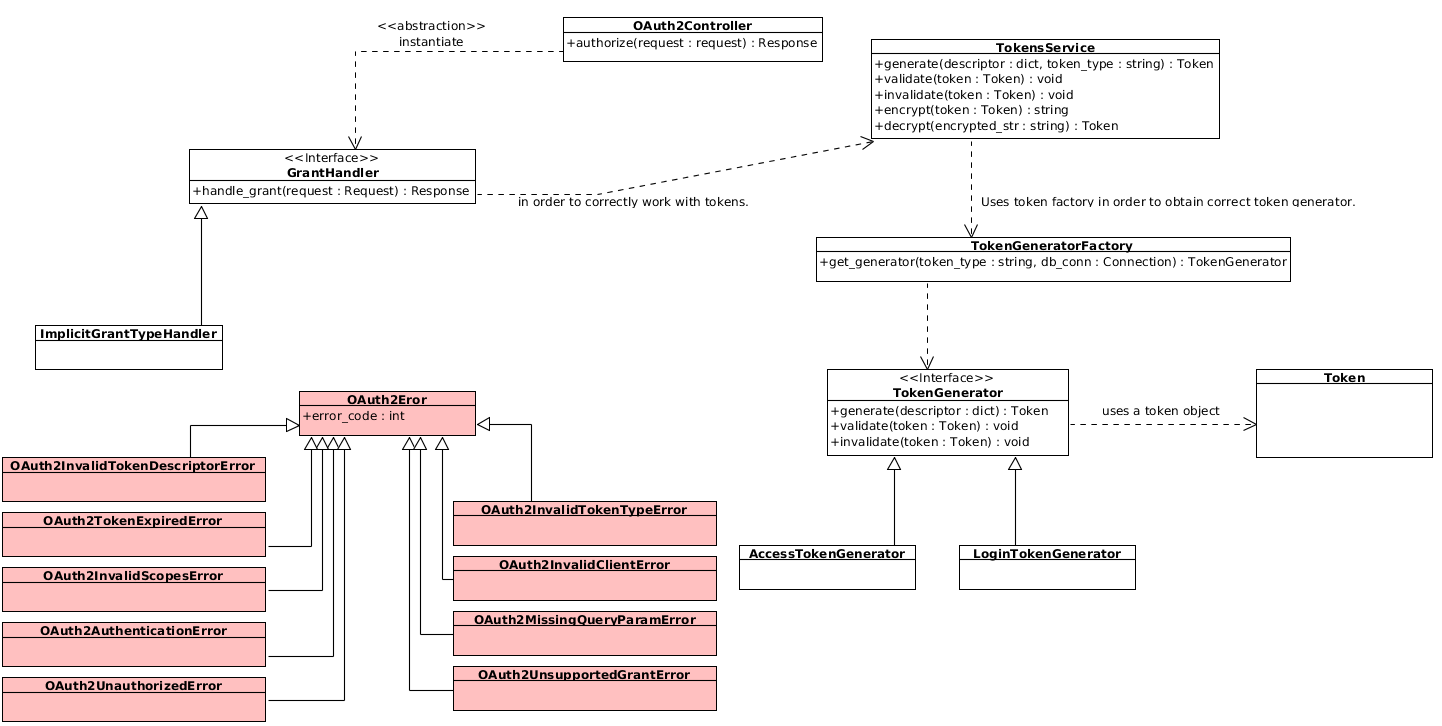
\includegraphics{oauth2_overview.png}
\index{handle\_authorize() (fantastico.oauth2.oauth2\_controller.OAuth2Controller method)}

\begin{fulllineitems}
\phantomsection\label{features/oauth2/technical_summary:fantastico.oauth2.oauth2_controller.OAuth2Controller.handle_authorize}\pysiglinewithargsret{\bfcode{handle\_authorize}}{\emph{*args}, \emph{**kwargs}}{}
This method provides the /authorize endpoint compliant with \href{http://tools.ietf.org/html/rfc6749}{RFC6479} standard.
Authorize endpoint provides an API for obtaining an access token or an authorization code depending on the grant type.

\end{fulllineitems}

\index{handle\_token() (fantastico.oauth2.oauth2\_controller.OAuth2Controller method)}

\begin{fulllineitems}
\phantomsection\label{features/oauth2/technical_summary:fantastico.oauth2.oauth2_controller.OAuth2Controller.handle_token}\pysiglinewithargsret{\bfcode{handle\_token}}{\emph{request}}{}
This method provides the /token endpoint compliant with \href{http://tools.ietf.org/html/rfc6749}{RFC6479}.
Token endpoint provides an API for obtaining access tokens.

\end{fulllineitems}


\end{fulllineitems}

\index{OAuth2TokensMiddleware (class in fantastico.oauth2.middleware.tokens\_middleware)}

\begin{fulllineitems}
\phantomsection\label{features/oauth2/technical_summary:fantastico.oauth2.middleware.tokens_middleware.OAuth2TokensMiddleware}\pysiglinewithargsret{\strong{class }\code{fantastico.oauth2.middleware.tokens\_middleware.}\bfcode{OAuth2TokensMiddleware}}{\emph{app}, \emph{tokens\_service\_cls=\textless{}class `fantastico.oauth2.tokens\_service.TokensService'\textgreater{}}}{}
This class provides a middleware responsible for decoding an access token (if exists) and building a security context. It
is extremely import to configure this middleware to run after
{\hyperref[features/request_response:fantastico.middleware.request_middleware.RequestMiddleware]{\code{fantastico.middleware.request\_middleware.RequestMiddleware}}} and after
{\hyperref[features/mvc:fantastico.middleware.model_session_middleware.ModelSessionMiddleware]{\code{fantastico.middleware.model\_session\_middleware.ModelSessionMiddleware}}} because
it needs a valid request and connection manager saved in the current pipeline execution.

\end{fulllineitems}

\index{OAuth2ExceptionsMiddleware (class in fantastico.oauth2.middleware.exceptions\_middleware)}

\begin{fulllineitems}
\phantomsection\label{features/oauth2/technical_summary:fantastico.oauth2.middleware.exceptions_middleware.OAuth2ExceptionsMiddleware}\pysiglinewithargsret{\strong{class }\code{fantastico.oauth2.middleware.exceptions\_middleware.}\bfcode{OAuth2ExceptionsMiddleware}}{\emph{app}, \emph{settings\_facade\_cls=\textless{}class `fantastico.settings.SettingsFacade'\textgreater{}}, \emph{exceptions\_factory\_cls=\textless{}class `fantastico.exception\_formatters.ExceptionFormattersFactory'\textgreater{}}}{}
This class provides the support for dynamically casting OAuth2 errors into concrete error responses. At the moment
responses are returned only in english and have the format specified in RFC6749. Mainly, at each intercepted OAuth2
exceptions a json response is returned to the client.

\end{fulllineitems}

\index{SecurityContext (class in fantastico.oauth2.security\_context)}

\begin{fulllineitems}
\phantomsection\label{features/oauth2/technical_summary:fantastico.oauth2.security_context.SecurityContext}\pysiglinewithargsret{\strong{class }\code{fantastico.oauth2.security\_context.}\bfcode{SecurityContext}}{\emph{access\_token}, \emph{required\_scopes=None}}{}
This class provides the OAuth2 security context. Security context is available for each request and can be accessed
using the following code snippet:

\begin{Verbatim}[commandchars=\\\{\}]
\PYG{n+nd}{@Controller}\PYG{p}{(}\PYG{n}{url}\PYG{o}{=}\PYG{l+s}{\PYGZdq{}}\PYG{l+s}{/test/controller}\PYG{l+s}{\PYGZdq{}}\PYG{p}{)}
\PYG{k}{def} \PYG{n+nf}{handle\PYGZus{}request}\PYG{p}{(}\PYG{n+nb+bp}{self}\PYG{p}{,} \PYG{n}{request}\PYG{p}{)}\PYG{p}{:}
    \PYG{n}{security\PYGZus{}ctx} \PYG{o}{=} \PYG{n}{request}\PYG{o}{.}\PYG{n}{context}\PYG{o}{.}\PYG{n}{security}

    \PYG{c}{\PYGZsh{} do something with security context}
\end{Verbatim}
\index{access\_token (fantastico.oauth2.security\_context.SecurityContext attribute)}

\begin{fulllineitems}
\phantomsection\label{features/oauth2/technical_summary:fantastico.oauth2.security_context.SecurityContext.access_token}\pysigline{\bfcode{access\_token}}
This property returns the current access token passed to the current http request. Access token is already decoded
as documented in {\hyperref[features/oauth2/tokens_format::doc]{\emph{OAUTH2 Fantastico Tokens}}} (encrypted section).

\end{fulllineitems}

\index{required\_scopes (fantastico.oauth2.security\_context.SecurityContext attribute)}

\begin{fulllineitems}
\phantomsection\label{features/oauth2/technical_summary:fantastico.oauth2.security_context.SecurityContext.required_scopes}\pysigline{\bfcode{required\_scopes}}
This property returns the current required scopes for http request. Required scopes are only available at runtime.

\end{fulllineitems}

\index{validate\_context() (fantastico.oauth2.security\_context.SecurityContext method)}

\begin{fulllineitems}
\phantomsection\label{features/oauth2/technical_summary:fantastico.oauth2.security_context.SecurityContext.validate_context}\pysiglinewithargsret{\bfcode{validate\_context}}{\emph{attr\_scope='scopes'}}{}
This method tries to validate the current security context using the current access token and required scopes.
Internally, the method simply ensures required scopes are present in access token granted scopes. Moreover, it receives
an optional parameter which allows requester to decide what section of required scopes it wants to validates. Valid
values are: scopes, create\_scopes, read\_scopes, update\_scopes or delete\_scopes.

\end{fulllineitems}


\end{fulllineitems}



\paragraph{Enforcing authorization}
\label{features/oauth2/technical_summary:enforcing-authorization}\index{RequiredScopes (class in fantastico.oauth2.oauth2\_decorators)}

\begin{fulllineitems}
\phantomsection\label{features/oauth2/technical_summary:fantastico.oauth2.oauth2_decorators.RequiredScopes}\pysiglinewithargsret{\strong{class }\code{fantastico.oauth2.oauth2\_decorators.}\bfcode{RequiredScopes}}{\emph{scopes=None}, \emph{create=None}, \emph{read=None}, \emph{update=None}, \emph{delete=None}}{}
This class provides the decorator for enforcing fantastico to authorize requests against ROA resources and MVC controllers.

\begin{Verbatim}[commandchars=\\\{\}]
\PYG{c}{\PYGZsh{} enforce authorization for MVC controllers.}
\PYG{n+nd}{@ControllerProvider}\PYG{p}{(}\PYG{p}{)}
\PYG{k}{class} \PYG{n+nc}{SecuredController}\PYG{p}{(}\PYG{n}{BaseController}\PYG{p}{)}\PYG{p}{:}
    \PYG{n+nd}{@Controller}\PYG{p}{(}\PYG{n}{url}\PYG{o}{=}\PYG{l+s}{\PYGZdq{}}\PYG{l+s}{/secured\PYGZhy{}controller/ui/index}\PYG{l+s}{\PYGZdq{}}\PYG{p}{)}
    \PYG{n+nd}{@RequiredScopes}\PYG{p}{(}\PYG{n}{scopes}\PYG{o}{=}\PYG{p}{[}\PYG{l+s}{\PYGZdq{}}\PYG{l+s}{greet.verbose}\PYG{l+s}{\PYGZdq{}}\PYG{p}{,} \PYG{l+s}{\PYGZdq{}}\PYG{l+s}{greet.read}\PYG{l+s}{\PYGZdq{}}\PYG{p}{]}\PYG{p}{)}
    \PYG{k}{def} \PYG{n+nf}{say\PYGZus{}hello}\PYG{p}{(}\PYG{n+nb+bp}{self}\PYG{p}{,} \PYG{n}{request}\PYG{p}{)}\PYG{p}{:}
        \PYG{k}{return} \PYG{l+s}{\PYGZdq{}}\PYG{l+s}{\PYGZlt{}html\PYGZgt{}\PYGZlt{}body\PYGZgt{}\PYGZlt{}h1\PYGZgt{}Hello world\PYGZlt{}/body\PYGZgt{}\PYGZlt{}/html\PYGZgt{}}\PYG{l+s}{\PYGZdq{}}
\end{Verbatim}

\begin{Verbatim}[commandchars=\\\{\}]
\PYG{c}{\PYGZsh{} enforce authorization for ROA resources.}
\PYG{n+nd}{@Resource}\PYG{p}{(}\PYG{n}{name}\PYG{o}{=}\PYG{l+s}{\PYGZdq{}}\PYG{l+s}{app\PYGZhy{}setting}\PYG{l+s}{\PYGZdq{}}\PYG{p}{,} \PYG{n}{url}\PYG{o}{=}\PYG{l+s}{\PYGZdq{}}\PYG{l+s}{/app\PYGZhy{}settings}\PYG{l+s}{\PYGZdq{}}\PYG{p}{,} \PYG{n}{version}\PYG{o}{=}\PYG{l+m+mf}{1.0}\PYG{p}{)}
\PYG{n+nd}{@RequiredScopes}\PYG{p}{(}\PYG{n}{create}\PYG{o}{=}\PYG{l+s}{\PYGZdq{}}\PYG{l+s}{app\PYGZus{}setting.create}\PYG{l+s}{\PYGZdq{}}\PYG{p}{,}
                \PYG{n}{read}\PYG{o}{=}\PYG{l+s}{\PYGZdq{}}\PYG{l+s}{app\PYGZus{}setting.read}\PYG{l+s}{\PYGZdq{}}\PYG{p}{,}
                \PYG{n}{update}\PYG{o}{=}\PYG{l+s}{\PYGZdq{}}\PYG{l+s}{app\PYGZus{}setting.update}\PYG{l+s}{\PYGZdq{}}\PYG{p}{,}
                \PYG{n}{delete}\PYG{o}{=}\PYG{l+s}{\PYGZdq{}}\PYG{l+s}{app\PYGZus{}setting.delete}\PYG{l+s}{\PYGZdq{}}\PYG{p}{\PYGZcb{}}\PYG{p}{)}
\PYG{k}{class} \PYG{n+nc}{AppSetting}\PYG{p}{(}\PYG{n}{BASEMODEL}\PYG{p}{)}\PYG{p}{:}
    \PYG{n+nb}{id} \PYG{o}{=} \PYG{n}{Column}\PYG{p}{(}\PYG{l+s}{\PYGZdq{}}\PYG{l+s}{id}\PYG{l+s}{\PYGZdq{}}\PYG{p}{,} \PYG{n}{Integer}\PYG{p}{,} \PYG{n}{primary\PYGZus{}key}\PYG{o}{=}\PYG{n+nb+bp}{True}\PYG{p}{,} \PYG{n}{autoincrement}\PYG{o}{=}\PYG{n+nb+bp}{True}\PYG{p}{)}
    \PYG{n}{name} \PYG{o}{=} \PYG{n}{Column}\PYG{p}{(}\PYG{l+s}{\PYGZdq{}}\PYG{l+s}{name}\PYG{l+s}{\PYGZdq{}}\PYG{p}{,} \PYG{n}{String}\PYG{p}{(}\PYG{l+m+mi}{50}\PYG{p}{)}\PYG{p}{,} \PYG{n}{unique}\PYG{o}{=}\PYG{n+nb+bp}{True}\PYG{p}{,} \PYG{n}{nullable}\PYG{o}{=}\PYG{n+nb+bp}{False}\PYG{p}{)}
    \PYG{n}{value} \PYG{o}{=} \PYG{n}{Column}\PYG{p}{(}\PYG{l+s}{\PYGZdq{}}\PYG{l+s}{value}\PYG{l+s}{\PYGZdq{}}\PYG{p}{,} \PYG{n}{Text}\PYG{p}{,} \PYG{n}{nullable}\PYG{o}{=}\PYG{n+nb+bp}{False}\PYG{p}{)}

    \PYG{k}{def} \PYG{n+nf}{\PYGZus{}\PYGZus{}init\PYGZus{}\PYGZus{}}\PYG{p}{(}\PYG{n+nb+bp}{self}\PYG{p}{,} \PYG{n}{name}\PYG{p}{,} \PYG{n}{value}\PYG{p}{)}\PYG{p}{:}
        \PYG{n+nb+bp}{self}\PYG{o}{.}\PYG{n}{name} \PYG{o}{=} \PYG{n}{name}
        \PYG{n+nb+bp}{self}\PYG{o}{.}\PYG{n}{value} \PYG{o}{=} \PYG{n}{value}
\end{Verbatim}
\index{create\_scopes (fantastico.oauth2.oauth2\_decorators.RequiredScopes attribute)}

\begin{fulllineitems}
\phantomsection\label{features/oauth2/technical_summary:fantastico.oauth2.oauth2_decorators.RequiredScopes.create_scopes}\pysigline{\bfcode{create\_scopes}}
This property returns the scopes required for create calls.

\end{fulllineitems}

\index{delete\_scopes (fantastico.oauth2.oauth2\_decorators.RequiredScopes attribute)}

\begin{fulllineitems}
\phantomsection\label{features/oauth2/technical_summary:fantastico.oauth2.oauth2_decorators.RequiredScopes.delete_scopes}\pysigline{\bfcode{delete\_scopes}}
This property returns the scopes required for delete calls.

\end{fulllineitems}

\index{inject\_scopes\_in\_security() (fantastico.oauth2.oauth2\_decorators.RequiredScopes method)}

\begin{fulllineitems}
\phantomsection\label{features/oauth2/technical_summary:fantastico.oauth2.oauth2_decorators.RequiredScopes.inject_scopes_in_security}\pysiglinewithargsret{\bfcode{inject\_scopes\_in\_security}}{\emph{request}}{}
This method injects the request scopes into request security context.

\end{fulllineitems}

\index{read\_scopes (fantastico.oauth2.oauth2\_decorators.RequiredScopes attribute)}

\begin{fulllineitems}
\phantomsection\label{features/oauth2/technical_summary:fantastico.oauth2.oauth2_decorators.RequiredScopes.read_scopes}\pysigline{\bfcode{read\_scopes}}
This property returns the scopes required for read calls.

\end{fulllineitems}

\index{scopes (fantastico.oauth2.oauth2\_decorators.RequiredScopes attribute)}

\begin{fulllineitems}
\phantomsection\label{features/oauth2/technical_summary:fantastico.oauth2.oauth2_decorators.RequiredScopes.scopes}\pysigline{\bfcode{scopes}}
This property returns the currently set scopes (including create, read, update, delete).

\end{fulllineitems}

\index{update\_scopes (fantastico.oauth2.oauth2\_decorators.RequiredScopes attribute)}

\begin{fulllineitems}
\phantomsection\label{features/oauth2/technical_summary:fantastico.oauth2.oauth2_decorators.RequiredScopes.update_scopes}\pysigline{\bfcode{update\_scopes}}
This property returns the scopes required for update calls.

\end{fulllineitems}


\end{fulllineitems}



\paragraph{Common tokens usage}
\label{features/oauth2/technical_summary:common-tokens-usage}

\subparagraph{Obtain authenticated user id}
\label{features/oauth2/technical_summary:obtain-authenticated-user-id}
It is common in web applications to want to obtain the current authenticated user unique identifier so that additional information
can be obtained in a secure context.
\begin{quote}

\begin{Verbatim}[commandchars=\\\{\}]
\PYG{n+nd}{@Controller}\PYG{p}{(}\PYG{n}{url}\PYG{o}{=}\PYG{l+s}{\PYGZdq{}}\PYG{l+s}{\PYGZca{}/users/ui/show\PYGZhy{}profile\PYGZdl{}}\PYG{l+s}{\PYGZdq{}}\PYG{p}{)}
\PYG{k}{def} \PYG{n+nf}{show\PYGZus{}profile}\PYG{p}{(}\PYG{n+nb+bp}{self}\PYG{p}{,} \PYG{n}{request}\PYG{p}{)}\PYG{p}{:}
   \PYG{n}{security\PYGZus{}ctx} \PYG{o}{=} \PYG{n}{request}\PYG{o}{.}\PYG{n}{context}\PYG{o}{.}\PYG{n}{security}
   \PYG{n}{user\PYGZus{}id} \PYG{o}{=} \PYG{n}{security\PYGZus{}ctx}\PYG{o}{.}\PYG{n}{access\PYGZus{}token}\PYG{o}{.}\PYG{n}{user\PYGZus{}id}

   \PYG{c}{\PYGZsh{} use profile endpoint to obtain additional information.}
\end{Verbatim}
\end{quote}


\subparagraph{Obtain current granted scopes}
\label{features/oauth2/technical_summary:obtain-current-granted-scopes}
It is common to want to access currently granted scopes for a given request. In order to do this use the following code snippet:
\begin{quote}

\begin{Verbatim}[commandchars=\\\{\}]
\PYG{n+nd}{@Controller}\PYG{p}{(}\PYG{n}{url}\PYG{o}{=}\PYG{l+s}{\PYGZdq{}}\PYG{l+s}{\PYGZca{}/sample\PYGZhy{}controller\PYGZdl{}}\PYG{l+s}{\PYGZdq{}}\PYG{p}{)}
\PYG{n+nd}{@RequiredScopes}\PYG{p}{(}\PYG{n}{scopes}\PYG{o}{=}\PYG{p}{[}\PYG{l+s}{\PYGZdq{}}\PYG{l+s}{custom\PYGZus{}scope1.read}\PYG{l+s}{\PYGZdq{}}\PYG{p}{]}\PYG{p}{)}
\PYG{k}{def} \PYG{n+nf}{handle\PYGZus{}request}\PYG{p}{(}\PYG{n+nb+bp}{self}\PYG{p}{,} \PYG{n}{request}\PYG{p}{)}\PYG{p}{:}
   \PYG{n}{access\PYGZus{}token} \PYG{o}{=} \PYG{n}{request}\PYG{o}{.}\PYG{n}{context}\PYG{o}{.}\PYG{n}{security}\PYG{o}{.}\PYG{n}{access\PYGZus{}token}
   \PYG{n}{scopes} \PYG{o}{=} \PYG{n}{access\PYGZus{}token}\PYG{o}{.}\PYG{n}{scopes}

   \PYG{c}{\PYGZsh{} validate scopes}
\end{Verbatim}
\end{quote}

If you try to use access token property of security context when no access token is expected this will be None.


\paragraph{Supported token generators}
\label{features/oauth2/technical_summary:supported-token-generators}\index{Token (class in fantastico.oauth2.token)}

\begin{fulllineitems}
\phantomsection\label{features/oauth2/technical_summary:fantastico.oauth2.token.Token}\pysiglinewithargsret{\strong{class }\code{fantastico.oauth2.token.}\bfcode{Token}}{\emph{desc}, \emph{immutable=True}}{}
This class provides a token model which can be built from a generic dictionary. All dictionary keys become token
members.

\end{fulllineitems}

\index{TokensService (class in fantastico.oauth2.tokens\_service)}

\begin{fulllineitems}
\phantomsection\label{features/oauth2/technical_summary:fantastico.oauth2.tokens_service.TokensService}\pysiglinewithargsret{\strong{class }\code{fantastico.oauth2.tokens\_service.}\bfcode{TokensService}}{\emph{db\_conn}, \emph{factory\_cls=\textless{}class `fantastico.oauth2.tokengenerator\_factory.TokenGeneratorFactory'\textgreater{}}, \emph{client\_repo\_cls=\textless{}class `fantastico.oauth2.models.client\_repository.ClientRepository'\textgreater{}}, \emph{encryptor\_cls=\textless{}class `fantastico.oauth2.token\_encryption.PublicTokenEncryption'\textgreater{}}}{}
This class provides an abstraction for working with all supported token types. Internally it uses
{\hyperref[features/oauth2/technical_summary:fantastico.oauth2.tokengenerator_factory.TokenGeneratorFactory]{\code{fantastico.oauth2.tokengenerator\_factory.TokenGeneratorFactory}}} for obtaining a correct token generator. Then,
it delegates all calls to that token generator.
\index{db\_conn (fantastico.oauth2.tokens\_service.TokensService attribute)}

\begin{fulllineitems}
\phantomsection\label{features/oauth2/technical_summary:fantastico.oauth2.tokens_service.TokensService.db_conn}\pysigline{\bfcode{db\_conn}}
This property returns the database connection used by this token service.

\end{fulllineitems}

\index{decrypt() (fantastico.oauth2.tokens\_service.TokensService method)}

\begin{fulllineitems}
\phantomsection\label{features/oauth2/technical_summary:fantastico.oauth2.tokens_service.TokensService.decrypt}\pysiglinewithargsret{\bfcode{decrypt}}{\emph{encrypted\_str}}{}
This method decrypts a given string and returns a concrete token object.

\end{fulllineitems}

\index{encrypt() (fantastico.oauth2.tokens\_service.TokensService method)}

\begin{fulllineitems}
\phantomsection\label{features/oauth2/technical_summary:fantastico.oauth2.tokens_service.TokensService.encrypt}\pysiglinewithargsret{\bfcode{encrypt}}{\emph{token}, \emph{client\_id}}{}
This method encrypts a given token and returns the encrypted string representation. Client id is required in order
to obtain the encryption keys.

\end{fulllineitems}

\index{generate() (fantastico.oauth2.tokens\_service.TokensService method)}

\begin{fulllineitems}
\phantomsection\label{features/oauth2/technical_summary:fantastico.oauth2.tokens_service.TokensService.generate}\pysiglinewithargsret{\bfcode{generate}}{\emph{token\_desc}, \emph{token\_type}}{}
This method generates a concrete token from the given token descriptor. It uses token\_type in order to choose the right
token generator.

\begin{Verbatim}[commandchars=\\\{\}]
\PYG{c}{\PYGZsh{} extract db\PYGZus{}conn from one of your controller injected facade models.}

\PYG{c}{\PYGZsh{} generate a new access token}
\PYG{n}{tokens\PYGZus{}service} \PYG{o}{=} \PYG{n}{TokensService}\PYG{p}{(}\PYG{n}{db\PYGZus{}conn}\PYG{p}{)}

\PYG{n}{token\PYGZus{}desc} \PYG{o}{=} \PYG{p}{\PYGZob{}}\PYG{l+s}{\PYGZdq{}}\PYG{l+s}{client\PYGZus{}id}\PYG{l+s}{\PYGZdq{}}\PYG{p}{:} \PYG{l+s}{\PYGZdq{}}\PYG{l+s}{sample\PYGZhy{}client}\PYG{l+s}{\PYGZdq{}}\PYG{p}{,}
              \PYG{l+s}{\PYGZdq{}}\PYG{l+s}{user\PYGZus{}id}\PYG{l+s}{\PYGZdq{}}\PYG{p}{:} \PYG{l+m+mi}{123}\PYG{p}{,}
              \PYG{l+s}{\PYGZdq{}}\PYG{l+s}{scopes}\PYG{l+s}{\PYGZdq{}}\PYG{p}{:} \PYG{l+s}{\PYGZdq{}}\PYG{l+s}{scope1 scope2 scope3}\PYG{l+s}{\PYGZdq{}}\PYG{p}{,}
              \PYG{l+s}{\PYGZdq{}}\PYG{l+s}{expires\PYGZus{}in}\PYG{l+s}{\PYGZdq{}}\PYG{p}{:} \PYG{l+m+mi}{3600}\PYG{p}{\PYGZcb{}}
\PYG{n}{access\PYGZus{}token} \PYG{o}{=} \PYG{n}{tokens\PYGZus{}service}\PYG{o}{.}\PYG{n}{generate}\PYG{p}{(}\PYG{n}{token\PYGZus{}desc}\PYG{p}{,} \PYG{n}{TokenGeneratorFactory}\PYG{o}{.}\PYG{n}{ACCESS\PYGZus{}TOKEN}\PYG{p}{)}
\end{Verbatim}

\end{fulllineitems}

\index{invalidate() (fantastico.oauth2.tokens\_service.TokensService method)}

\begin{fulllineitems}
\phantomsection\label{features/oauth2/technical_summary:fantastico.oauth2.tokens_service.TokensService.invalidate}\pysiglinewithargsret{\bfcode{invalidate}}{\emph{token}}{}
This method invalidates a given token object. For instance, authorization codes can be invalidated. In order to
invalidate a token you can use the code snippet below:

\begin{Verbatim}[commandchars=\\\{\}]
\PYG{c}{\PYGZsh{} extract db\PYGZus{}conn from one of your controller injected facade models.}
\PYG{c}{\PYGZsh{} extract token from request or instantiate a new token.}

\PYG{n}{tokens\PYGZus{}service} \PYG{o}{=} \PYG{n}{TokensService}\PYG{p}{(}\PYG{n}{db\PYGZus{}conn}\PYG{p}{)}
\PYG{n}{tokens\PYGZus{}service}\PYG{o}{.}\PYG{n}{invalidate}\PYG{p}{(}\PYG{n}{token}\PYG{p}{)}
\end{Verbatim}

\end{fulllineitems}

\index{validate() (fantastico.oauth2.tokens\_service.TokensService method)}

\begin{fulllineitems}
\phantomsection\label{features/oauth2/technical_summary:fantastico.oauth2.tokens_service.TokensService.validate}\pysiglinewithargsret{\bfcode{validate}}{\emph{token}}{}
This method validates a given token object. Internally, a generator is selected to validate the given token based on
the given token type.

\begin{Verbatim}[commandchars=\\\{\}]
\PYG{c}{\PYGZsh{} extract db\PYGZus{}conn from one of your controller injected facade models.}
\PYG{c}{\PYGZsh{} extract token from request or instantiate a new token.}

\PYG{n}{tokens\PYGZus{}service} \PYG{o}{=} \PYG{n}{TokensService}\PYG{p}{(}\PYG{n}{db\PYGZus{}conn}\PYG{p}{)}
\PYG{n}{tokens\PYGZus{}service}\PYG{o}{.}\PYG{n}{validate}\PYG{p}{(}\PYG{n}{token}\PYG{p}{)}
\end{Verbatim}

\end{fulllineitems}


\end{fulllineitems}

\index{TokenGeneratorFactory (class in fantastico.oauth2.tokengenerator\_factory)}

\begin{fulllineitems}
\phantomsection\label{features/oauth2/technical_summary:fantastico.oauth2.tokengenerator_factory.TokenGeneratorFactory}\pysigline{\strong{class }\code{fantastico.oauth2.tokengenerator\_factory.}\bfcode{TokenGeneratorFactory}}
This class provides the entry point for working with generators. It provides a factory for easily instantiating a generator
which can work with a request token type.

\begin{Verbatim}[commandchars=\\\{\}]
\PYG{n}{login\PYGZus{}generator} \PYG{o}{=} \PYG{n}{TokenGeneratorFactory}\PYG{p}{(}\PYG{p}{)}\PYG{o}{.}\PYG{n}{get\PYGZus{}generator}\PYG{p}{(}\PYG{n}{TokenGeneratorFactory}\PYG{o}{.}\PYG{n}{LOGIN\PYGZus{}TOKEN}\PYG{p}{)}
\end{Verbatim}
\index{get\_generator() (fantastico.oauth2.tokengenerator\_factory.TokenGeneratorFactory method)}

\begin{fulllineitems}
\phantomsection\label{features/oauth2/technical_summary:fantastico.oauth2.tokengenerator_factory.TokenGeneratorFactory.get_generator}\pysiglinewithargsret{\bfcode{get\_generator}}{\emph{token\_type}, \emph{db\_conn}}{}
This method returns an instance of a token generator which can handel requested token type.
\begin{quote}\begin{description}
\item[{Parameters}] \leavevmode\begin{itemize}
\item {} 
\textbf{token\_type} (\emph{string}) -- A unique token type.

\item {} 
\textbf{db\_conn} -- An existing database connection (sql alchemy object) used when working with client context.

\end{itemize}

\item[{Returns}] \leavevmode
An instance of a concrete token generator which is compatible with the request token type.

\item[{Return type}] \leavevmode
{\hyperref[features/oauth2/technical_summary:fantastico.oauth2.token_generator.TokenGenerator]{\code{fantastico.oauth2.token\_generator.TokenGenerator}}}

\end{description}\end{quote}

\end{fulllineitems}


\end{fulllineitems}

\index{TokenGenerator (class in fantastico.oauth2.token\_generator)}

\begin{fulllineitems}
\phantomsection\label{features/oauth2/technical_summary:fantastico.oauth2.token_generator.TokenGenerator}\pysiglinewithargsret{\strong{class }\code{fantastico.oauth2.token\_generator.}\bfcode{TokenGenerator}}{\emph{db\_conn}, \emph{model\_facade\_cls=\textless{}class `fantastico.mvc.model\_facade.ModelFacade'\textgreater{}}}{}
This class provides an abstract contract which must be provided by each concrete token generator. A token generator
must provide the following functionality:
\begin{itemize}
\item {} 
generate a new token

\item {} 
validate a given token

\item {} 
invalidate a given token

\end{itemize}
\index{generate() (fantastico.oauth2.token\_generator.TokenGenerator method)}

\begin{fulllineitems}
\phantomsection\label{features/oauth2/technical_summary:fantastico.oauth2.token_generator.TokenGenerator.generate}\pysiglinewithargsret{\bfcode{generate}}{\emph{token\_desc}}{}
This method must be overriden so that it builds a correct token from the given descriptor. Descriptor is a free
form object.
\begin{quote}\begin{description}
\item[{Parameters}] \leavevmode
\textbf{token\_desc} (\emph{dict}) -- A dictionary containing all keys required for generating a new token.

\item[{Returns}] \leavevmode
A new token object.

\item[{Return type}] \leavevmode
{\hyperref[features/oauth2/technical_summary:fantastico.oauth2.token.Token]{\code{fantastico.oauth2.token.Token}}}

\end{description}\end{quote}

\end{fulllineitems}

\index{invalidate() (fantastico.oauth2.token\_generator.TokenGenerator method)}

\begin{fulllineitems}
\phantomsection\label{features/oauth2/technical_summary:fantastico.oauth2.token_generator.TokenGenerator.invalidate}\pysiglinewithargsret{\bfcode{invalidate}}{\emph{token}}{}
This method must be overriden if the given token supports invalidation (e.g: authorization code). In many cases
this is not necessary so this is a nop.

\end{fulllineitems}

\index{validate() (fantastico.oauth2.token\_generator.TokenGenerator method)}

\begin{fulllineitems}
\phantomsection\label{features/oauth2/technical_summary:fantastico.oauth2.token_generator.TokenGenerator.validate}\pysiglinewithargsret{\bfcode{validate}}{\emph{token}}{}
This method must be overriden so that it validates the given token. Usually, if the token is not valid a concrete
exception must be raised.
\begin{quote}\begin{description}
\item[{Parameters}] \leavevmode
\textbf{token} ({\hyperref[features/oauth2/technical_summary:fantastico.oauth2.token.Token]{\code{fantastico.oauth2.token.Token}}}) -- The token object we want to validate.

\end{description}\end{quote}

\end{fulllineitems}


\end{fulllineitems}

\index{LoginTokenGenerator (class in fantastico.oauth2.logintoken\_generator)}

\begin{fulllineitems}
\phantomsection\label{features/oauth2/technical_summary:fantastico.oauth2.logintoken_generator.LoginTokenGenerator}\pysiglinewithargsret{\strong{class }\code{fantastico.oauth2.logintoken\_generator.}\bfcode{LoginTokenGenerator}}{\emph{db\_conn}, \emph{model\_facade\_cls=\textless{}class `fantastico.mvc.model\_facade.ModelFacade'\textgreater{}}}{}
This class provides support for generating and working with login tokens. A login token is used for proving that a user
is authenticated correctly. For more information, read {\hyperref[features/oauth2/tokens_format::doc]{\emph{OAUTH2 Fantastico Tokens}}}.
\index{generate() (fantastico.oauth2.logintoken\_generator.LoginTokenGenerator method)}

\begin{fulllineitems}
\phantomsection\label{features/oauth2/technical_summary:fantastico.oauth2.logintoken_generator.LoginTokenGenerator.generate}\pysiglinewithargsret{\bfcode{generate}}{\emph{token\_desc}, \emph{time\_provider=\textless{}module `time' (built-in)\textgreater{}}}{}
This method generates a login token. In order to succeed token descriptor must contain the following keys:
\begin{itemize}
\item {} 
client\_id - a unique identifier for the idp which generated the token.

\item {} 
user\_id - idp user unique identifier.

\item {} 
expires\_in - an integer value in seconds determining the maximum validity of the token.

\end{itemize}

If any of the above keys are missing an oauth 2 exception is raised.

\end{fulllineitems}

\index{validate() (fantastico.oauth2.logintoken\_generator.LoginTokenGenerator method)}

\begin{fulllineitems}
\phantomsection\label{features/oauth2/technical_summary:fantastico.oauth2.logintoken_generator.LoginTokenGenerator.validate}\pysiglinewithargsret{\bfcode{validate}}{\emph{token}}{}
This method checks the given login token for:
\begin{itemize}
\item {} 
correct type (login).

\item {} 
expiration time.

\end{itemize}

\end{fulllineitems}


\end{fulllineitems}

\index{AccessTokenGenerator (class in fantastico.oauth2.accesstoken\_generator)}

\begin{fulllineitems}
\phantomsection\label{features/oauth2/technical_summary:fantastico.oauth2.accesstoken_generator.AccessTokenGenerator}\pysiglinewithargsret{\strong{class }\code{fantastico.oauth2.accesstoken\_generator.}\bfcode{AccessTokenGenerator}}{\emph{db\_conn}, \emph{model\_facade\_cls=\textless{}class `fantastico.mvc.model\_facade.ModelFacade'\textgreater{}}}{}
This class provides the methods for working with access tokens: (generate and validate).
\index{generate() (fantastico.oauth2.accesstoken\_generator.AccessTokenGenerator method)}

\begin{fulllineitems}
\phantomsection\label{features/oauth2/technical_summary:fantastico.oauth2.accesstoken_generator.AccessTokenGenerator.generate}\pysiglinewithargsret{\bfcode{generate}}{\emph{token\_desc}, \emph{time\_provider=\textless{}module `time' (built-in)\textgreater{}}}{}
This method generates a new access token starting from the givent token descriptor. In order to succeed the token
descriptor must contain the following keys:
\begin{itemize}
\item {} 
client\_id - Client unique identifier.

\item {} 
user\_id - User unique identifier.

\item {} 
scopes - The scopes requested for this client (a space delimited list of strings).

\item {} 
expires\_in - The time to live period (in seconds) for the newly generated access token.

\end{itemize}

\end{fulllineitems}

\index{validate() (fantastico.oauth2.accesstoken\_generator.AccessTokenGenerator method)}

\begin{fulllineitems}
\phantomsection\label{features/oauth2/technical_summary:fantastico.oauth2.accesstoken_generator.AccessTokenGenerator.validate}\pysiglinewithargsret{\bfcode{validate}}{\emph{token}}{}
This method validates a given access token. It checks for:
\begin{itemize}
\item {} 
valid client id

\item {} 
valid token type

\item {} 
token not expired

\end{itemize}

\end{fulllineitems}


\end{fulllineitems}



\paragraph{Encryption / decryption}
\label{features/oauth2/technical_summary:encryption-decryption}
In Fantastico OAuth2, tokens are encrypted / decrypted using AES symmetric encryption. Below you can find the classes which provides
AES implementation:
\index{TokenEncryption (class in fantastico.oauth2.token\_encryption)}

\begin{fulllineitems}
\phantomsection\label{features/oauth2/technical_summary:fantastico.oauth2.token_encryption.TokenEncryption}\pysigline{\strong{class }\code{fantastico.oauth2.token\_encryption.}\bfcode{TokenEncryption}}
This class provides an abstract model for token encryption providers. A token encryption provider must be able
to encrypt / decrypt a {\hyperref[features/oauth2/technical_summary:fantastico.oauth2.token.Token]{\code{fantastico.oauth2.token.Token}}} objects.
\index{decrypt\_token() (fantastico.oauth2.token\_encryption.TokenEncryption method)}

\begin{fulllineitems}
\phantomsection\label{features/oauth2/technical_summary:fantastico.oauth2.token_encryption.TokenEncryption.decrypt_token}\pysiglinewithargsret{\bfcode{decrypt\_token}}{\emph{encrypted\_str}, \emph{token\_iv}, \emph{token\_key}}{}
This method must be overriden by concrete providers in order to correctly transform an encrypted string into a token
object.
\begin{quote}\begin{description}
\item[{Parameters}] \leavevmode\begin{itemize}
\item {} 
\textbf{encrypted\_str} (\emph{str}) -- Encrypted token representation.

\item {} 
\textbf{token\_iv} (\emph{byte{[}{]}}) -- Token initialization vector used in symmetric encryption. Most of the times this will have a fix 128 bits length.

\item {} 
\textbf{token\_key} (\emph{byte{[}{]}}) -- Token key used in symmetric encryption. Based on the implementation the length might vary: 128 / 192 / 256 bits.

\end{itemize}

\item[{Returns}] \leavevmode
Decrypted token object.

\item[{Return type}] \leavevmode
{\hyperref[features/oauth2/technical_summary:fantastico.oauth2.token.Token]{\code{fantastico.oauth2.token.Token}}}

\end{description}\end{quote}

\end{fulllineitems}

\index{encrypt\_token() (fantastico.oauth2.token\_encryption.TokenEncryption method)}

\begin{fulllineitems}
\phantomsection\label{features/oauth2/technical_summary:fantastico.oauth2.token_encryption.TokenEncryption.encrypt_token}\pysiglinewithargsret{\bfcode{encrypt\_token}}{\emph{token}, \emph{token\_iv}, \emph{token\_key}}{}
This method must be overriden by concrete providers in order to correctly transform a token object into an encrypted
string.
\begin{quote}\begin{description}
\item[{Parameters}] \leavevmode\begin{itemize}
\item {} 
\textbf{token} ({\hyperref[features/oauth2/technical_summary:fantastico.oauth2.token.Token]{\code{fantastico.oauth2.token.Token}}}) -- A token object we want to encrypt.

\item {} 
\textbf{token\_iv} (\emph{byte{[}{]}}) -- Token initialization vector used in symmetric encryption. Most of the times this will have a fix 128 bits length.

\item {} 
\textbf{token\_key} (\emph{byte{[}{]}}) -- Token key used in symmetric encryption. Based on the implementation the length might vary: 128 / 192 / 256 bits.

\end{itemize}

\item[{Returns}] \leavevmode
The encrypted representation of the token.

\item[{Return type}] \leavevmode
str

\end{description}\end{quote}

\end{fulllineitems}


\end{fulllineitems}

\index{AesTokenEncryption (class in fantastico.oauth2.token\_encryption)}

\begin{fulllineitems}
\phantomsection\label{features/oauth2/technical_summary:fantastico.oauth2.token_encryption.AesTokenEncryption}\pysigline{\strong{class }\code{fantastico.oauth2.token\_encryption.}\bfcode{AesTokenEncryption}}
This class provides a generic AES token encryption provider. It allows developers to specify the number of bits used
for AES (128 / 192 / 256 bits).
\index{decrypt\_token() (fantastico.oauth2.token\_encryption.AesTokenEncryption method)}

\begin{fulllineitems}
\phantomsection\label{features/oauth2/technical_summary:fantastico.oauth2.token_encryption.AesTokenEncryption.decrypt_token}\pysiglinewithargsret{\bfcode{decrypt\_token}}{\emph{encrypted\_str}, \emph{token\_iv}, \emph{token\_key}}{}
This method uses AES for decrypting the given string. Internally, decrypted string is converted into a dictionary and
then into a concrete token object.

\end{fulllineitems}

\index{encrypt\_token() (fantastico.oauth2.token\_encryption.AesTokenEncryption method)}

\begin{fulllineitems}
\phantomsection\label{features/oauth2/technical_summary:fantastico.oauth2.token_encryption.AesTokenEncryption.encrypt_token}\pysiglinewithargsret{\bfcode{encrypt\_token}}{\emph{token}, \emph{token\_iv}, \emph{token\_key}}{}
This method uses AES for encrypting the given token. Internally it transform the token into a JSON string and
encrypt it using given token\_iv and token\_key.

\end{fulllineitems}


\end{fulllineitems}

\index{PublicTokenEncryption (class in fantastico.oauth2.token\_encryption)}

\begin{fulllineitems}
\phantomsection\label{features/oauth2/technical_summary:fantastico.oauth2.token_encryption.PublicTokenEncryption}\pysiglinewithargsret{\strong{class }\code{fantastico.oauth2.token\_encryption.}\bfcode{PublicTokenEncryption}}{\emph{symmetric\_encryptor}}{}
This class provides a special token encryption: a mix of base64 encoded and symmetrical encrypted token. We need
this mix because client\_id is required for every operation involving oauth2 tokens.
\index{decrypt\_token() (fantastico.oauth2.token\_encryption.PublicTokenEncryption method)}

\begin{fulllineitems}
\phantomsection\label{features/oauth2/technical_summary:fantastico.oauth2.token_encryption.PublicTokenEncryption.decrypt_token}\pysiglinewithargsret{\bfcode{decrypt\_token}}{\emph{encrypted\_str}, \emph{token\_iv=None}, \emph{token\_key=None}, \emph{client\_repo=None}}{}
This methods receives a public token representation and returns a concrete token object. In many cases token\_iv and
token\_key will not be known so they will obtained from the public part of the token using client\_id descriptor
persisted in database.

\end{fulllineitems}

\index{encrypt\_token() (fantastico.oauth2.token\_encryption.PublicTokenEncryption method)}

\begin{fulllineitems}
\phantomsection\label{features/oauth2/technical_summary:fantastico.oauth2.token_encryption.PublicTokenEncryption.encrypt_token}\pysiglinewithargsret{\bfcode{encrypt\_token}}{\emph{token}, \emph{token\_iv=None}, \emph{token\_key=None}, \emph{client\_repo=None}}{}
This method takes a concrete token object and returns a base64 representation of the token. In the rare cases where
the encryption vectors are not known client\_repo is used to read client descriptor and lazy obtain the vectors.

\end{fulllineitems}


\end{fulllineitems}



\paragraph{Suported grant types}
\label{features/oauth2/technical_summary:suported-grant-types}\index{GrantHandler (class in fantastico.oauth2.grant\_handler)}

\begin{fulllineitems}
\phantomsection\label{features/oauth2/technical_summary:fantastico.oauth2.grant_handler.GrantHandler}\pysiglinewithargsret{\strong{class }\code{fantastico.oauth2.grant\_handler.}\bfcode{GrantHandler}}{\emph{tokens\_service}, \emph{settings\_facade}}{}
This class provides the abstract contract of a handler. Each concrete handler must implement this contract in order to
correctly extend Fantastico OAuth2 supported handlers.
\index{handle\_grant() (fantastico.oauth2.grant\_handler.GrantHandler method)}

\begin{fulllineitems}
\phantomsection\label{features/oauth2/technical_summary:fantastico.oauth2.grant_handler.GrantHandler.handle_grant}\pysiglinewithargsret{\bfcode{handle\_grant}}{\emph{request}}{}
This method must be overriden in order to correctly implement grant logic. It receives the current http request
and return a http response.

\end{fulllineitems}


\end{fulllineitems}

\index{GrantHandlerFactory (class in fantastico.oauth2.grant\_handler\_factory)}

\begin{fulllineitems}
\phantomsection\label{features/oauth2/technical_summary:fantastico.oauth2.grant_handler_factory.GrantHandlerFactory}\pysiglinewithargsret{\strong{class }\code{fantastico.oauth2.grant\_handler\_factory.}\bfcode{GrantHandlerFactory}}{\emph{tokens\_service\_cls=\textless{}class `fantastico.oauth2.tokens\_service.TokensService'\textgreater{}}, \emph{settings\_facade\_cls=\textless{}class `fantastico.settings.SettingsFacade'\textgreater{}}}{}
This class provides a factory which can be used to obtain a concrete grant handler. Below you can find a code snippet for
obtaining and implicit grant type handler:

\begin{Verbatim}[commandchars=\\\{\}]
\PYG{n}{grant\PYGZus{}handler} \PYG{o}{=} \PYG{n}{GrantHandlerFactory}\PYG{p}{(}\PYG{p}{)}\PYG{o}{.}\PYG{n}{get\PYGZus{}handler}\PYG{p}{(}\PYG{n}{GrantHandlerFactory}\PYG{o}{.}\PYG{n}{IMPLICIT\PYGZus{}GRANT}\PYG{p}{)}
\end{Verbatim}
\index{get\_handler() (fantastico.oauth2.grant\_handler\_factory.GrantHandlerFactory method)}

\begin{fulllineitems}
\phantomsection\label{features/oauth2/technical_summary:fantastico.oauth2.grant_handler_factory.GrantHandlerFactory.get_handler}\pysiglinewithargsret{\bfcode{get\_handler}}{\emph{handler\_type}, \emph{db\_conn}}{}
This method builds a grant handler which matches requested handler\_type.
\begin{quote}\begin{description}
\item[{Parameters}] \leavevmode\begin{itemize}
\item {} 
\textbf{handler\_type} (\emph{str}) -- A string value describing the grant\_type which must be handled.

\item {} 
\textbf{db\_conn} (\emph{Connection}) -- A db connection active session which cn be used.

\end{itemize}

\item[{Returns}] \leavevmode
A concrete grant handler instance.

\item[{Return type}] \leavevmode
{\hyperref[features/oauth2/technical_summary:fantastico.oauth2.grant_handler.GrantHandler]{\code{fantastico.oauth2.grant\_handler.GrantHandler}}}

\end{description}\end{quote}

\end{fulllineitems}


\end{fulllineitems}

\index{ImplicitGrantHandler (class in fantastico.oauth2.implicit\_grant\_handler)}

\begin{fulllineitems}
\phantomsection\label{features/oauth2/technical_summary:fantastico.oauth2.implicit_grant_handler.ImplicitGrantHandler}\pysiglinewithargsret{\strong{class }\code{fantastico.oauth2.implicit\_grant\_handler.}\bfcode{ImplicitGrantHandler}}{\emph{tokens\_service}, \emph{settings\_facade}, \emph{exception\_formatters\_cls=\textless{}class `fantastico.exception\_formatters.ExceptionFormattersFactory'\textgreater{}}, \emph{client\_repo\_cls=\textless{}class `fantastico.oauth2.models.client\_repository.ClientRepository'\textgreater{}}}{}
This class provides the implementation for implicit grant type described in
\href{http://tools.ietf.org/html/rfc6749}{RFC6749}. Implementation of this grant type is fully compliant with 
OAuth2 spec. In addition to RFC6749, the implicit grant implemented in fantastico supports an additional
query parameter named \textbf{redirect} which is optional. If redirect query parameter is specified with value
0 then a 200 OK response is returned to the client in comparison with redirect 1 value where 302 Found response
is returned. We do this in order to support more advanced use cases where user can orchestrate the redirects
rather than browser.
\index{handle\_grant() (fantastico.oauth2.implicit\_grant\_handler.ImplicitGrantHandler method)}

\begin{fulllineitems}
\phantomsection\label{features/oauth2/technical_summary:fantastico.oauth2.implicit_grant_handler.ImplicitGrantHandler.handle_grant}\pysiglinewithargsret{\bfcode{handle\_grant}}{\emph{request}}{}
This method provides the algorithm for implementing implicit grant type handler. Internally it will use TokensService
in order to generate a new access token. In addition, if redirect query parameter is set to false then a 200 OK response
with Location header and no body is sent to the client.

\end{fulllineitems}


\end{fulllineitems}



\paragraph{Concrete exceptions}
\label{features/oauth2/technical_summary:concrete-exceptions}\index{OAuth2Error (class in fantastico.oauth2.exceptions)}

\begin{fulllineitems}
\phantomsection\label{features/oauth2/technical_summary:fantastico.oauth2.exceptions.OAuth2Error}\pysiglinewithargsret{\strong{class }\code{fantastico.oauth2.exceptions.}\bfcode{OAuth2Error}}{\emph{error\_code=12000}, \emph{msg=None}, \emph{http\_code=400}}{}
This class provides the base class for OAuth2 exceptions. In order to be compliant with
\href{http://tools.ietf.org/html/rfc6749}{OAuth2 spec} each oauth error is described by a status code, an error code and a
friendly description.
\index{error\_code (fantastico.oauth2.exceptions.OAuth2Error attribute)}

\begin{fulllineitems}
\phantomsection\label{features/oauth2/technical_summary:fantastico.oauth2.exceptions.OAuth2Error.error_code}\pysigline{\bfcode{error\_code}}
This property returns the exception error code.

\end{fulllineitems}


\end{fulllineitems}

\index{OAuth2InvalidTokenDescriptorError (class in fantastico.oauth2.exceptions)}

\begin{fulllineitems}
\phantomsection\label{features/oauth2/technical_summary:fantastico.oauth2.exceptions.OAuth2InvalidTokenDescriptorError}\pysiglinewithargsret{\strong{class }\code{fantastico.oauth2.exceptions.}\bfcode{OAuth2InvalidTokenDescriptorError}}{\emph{attr\_name}}{}
This class provides a concrete exception used to notify a missing attribute from a token descriptor.
\index{attr\_name (fantastico.oauth2.exceptions.OAuth2InvalidTokenDescriptorError attribute)}

\begin{fulllineitems}
\phantomsection\label{features/oauth2/technical_summary:fantastico.oauth2.exceptions.OAuth2InvalidTokenDescriptorError.attr_name}\pysigline{\bfcode{attr\_name}}
This property returns the missing attribute name.

\end{fulllineitems}


\end{fulllineitems}

\index{OAuth2InvalidTokenTypeError (class in fantastico.oauth2.exceptions)}

\begin{fulllineitems}
\phantomsection\label{features/oauth2/technical_summary:fantastico.oauth2.exceptions.OAuth2InvalidTokenTypeError}\pysiglinewithargsret{\strong{class }\code{fantastico.oauth2.exceptions.}\bfcode{OAuth2InvalidTokenTypeError}}{\emph{token\_type}, \emph{msg}}{}
This class provides a concrete exception used to notify that a token has been sent to a token generator which does not
support it or the token type is unknown.
\index{token\_type (fantastico.oauth2.exceptions.OAuth2InvalidTokenTypeError attribute)}

\begin{fulllineitems}
\phantomsection\label{features/oauth2/technical_summary:fantastico.oauth2.exceptions.OAuth2InvalidTokenTypeError.token_type}\pysigline{\bfcode{token\_type}}
This property returns the invalid token type.

\end{fulllineitems}


\end{fulllineitems}

\index{OAuth2TokenExpiredError (class in fantastico.oauth2.exceptions)}

\begin{fulllineitems}
\phantomsection\label{features/oauth2/technical_summary:fantastico.oauth2.exceptions.OAuth2TokenExpiredError}\pysiglinewithargsret{\strong{class }\code{fantastico.oauth2.exceptions.}\bfcode{OAuth2TokenExpiredError}}{\emph{msg=None}}{}
This class provides a concrete exception used to notify that a token is expired.

\end{fulllineitems}

\index{OAuth2InvalidClientError (class in fantastico.oauth2.exceptions)}

\begin{fulllineitems}
\phantomsection\label{features/oauth2/technical_summary:fantastico.oauth2.exceptions.OAuth2InvalidClientError}\pysiglinewithargsret{\strong{class }\code{fantastico.oauth2.exceptions.}\bfcode{OAuth2InvalidClientError}}{\emph{msg}}{}
This class provides a concrete exception used to notify an invalid client (not found or revoked).

\end{fulllineitems}

\index{OAuth2InvalidScopesError (class in fantastico.oauth2.exceptions)}

\begin{fulllineitems}
\phantomsection\label{features/oauth2/technical_summary:fantastico.oauth2.exceptions.OAuth2InvalidScopesError}\pysiglinewithargsret{\strong{class }\code{fantastico.oauth2.exceptions.}\bfcode{OAuth2InvalidScopesError}}{\emph{msg}}{}
This class provides a concrete exception used to notify that a client is not allowed to use a request set of scopes.

\end{fulllineitems}

\index{OAuth2MissingQueryParamError (class in fantastico.oauth2.exceptions)}

\begin{fulllineitems}
\phantomsection\label{features/oauth2/technical_summary:fantastico.oauth2.exceptions.OAuth2MissingQueryParamError}\pysiglinewithargsret{\strong{class }\code{fantastico.oauth2.exceptions.}\bfcode{OAuth2MissingQueryParamError}}{\emph{param\_name}}{}
This class provides a concrete exception used to notify a missing query parameter from an OAuth2 endpoint.
\index{param\_name (fantastico.oauth2.exceptions.OAuth2MissingQueryParamError attribute)}

\begin{fulllineitems}
\phantomsection\label{features/oauth2/technical_summary:fantastico.oauth2.exceptions.OAuth2MissingQueryParamError.param_name}\pysigline{\bfcode{param\_name}}
This property return the name of the query parameter which is missing.

\end{fulllineitems}


\end{fulllineitems}

\index{OAuth2TokenEncryptionError (class in fantastico.oauth2.exceptions)}

\begin{fulllineitems}
\phantomsection\label{features/oauth2/technical_summary:fantastico.oauth2.exceptions.OAuth2TokenEncryptionError}\pysiglinewithargsret{\strong{class }\code{fantastico.oauth2.exceptions.}\bfcode{OAuth2TokenEncryptionError}}{\emph{msg}}{}
This class provides a concrete exception used to notify an error during encrypt / decrypt token operations.

\end{fulllineitems}

\index{OAuth2UnsupportedGrantError (class in fantastico.oauth2.exceptions)}

\begin{fulllineitems}
\phantomsection\label{features/oauth2/technical_summary:fantastico.oauth2.exceptions.OAuth2UnsupportedGrantError}\pysiglinewithargsret{\strong{class }\code{fantastico.oauth2.exceptions.}\bfcode{OAuth2UnsupportedGrantError}}{\emph{handler\_type}}{}
This class provides a concrete exception for notifying unsupport oauth2 grant type.
\index{handler\_type (fantastico.oauth2.exceptions.OAuth2UnsupportedGrantError attribute)}

\begin{fulllineitems}
\phantomsection\label{features/oauth2/technical_summary:fantastico.oauth2.exceptions.OAuth2UnsupportedGrantError.handler_type}\pysigline{\bfcode{handler\_type}}
This property holds the unsupported grant type name.

\end{fulllineitems}


\end{fulllineitems}

\index{OAuth2UnauthorizedError (class in fantastico.oauth2.exceptions)}

\begin{fulllineitems}
\phantomsection\label{features/oauth2/technical_summary:fantastico.oauth2.exceptions.OAuth2UnauthorizedError}\pysiglinewithargsret{\strong{class }\code{fantastico.oauth2.exceptions.}\bfcode{OAuth2UnauthorizedError}}{\emph{msg}}{}
This class provides a concrete exception for notifying unauthorized access to oauth2 protected resources.

\end{fulllineitems}

\index{OAuth2AuthenticationError (class in fantastico.oauth2.exceptions)}

\begin{fulllineitems}
\phantomsection\label{features/oauth2/technical_summary:fantastico.oauth2.exceptions.OAuth2AuthenticationError}\pysiglinewithargsret{\strong{class }\code{fantastico.oauth2.exceptions.}\bfcode{OAuth2AuthenticationError}}{\emph{msg}, \emph{http\_code=403}}{}
This class provides a concrete exception used to notify a failed authentication attempt from an OAuth2 IDP.

\end{fulllineitems}



\subsection{OAuth2 exceptions}
\label{features/oauth2:oauth2-exceptions}

\subsubsection{12000 - OAuth generic error}
\label{features/oauth2/exceptions/12000:oauth-generic-error}\label{features/oauth2/exceptions/12000::doc}
This error can occur when something unexpected occured into OAuth /authorize or /token apis. Most of the time you should not
get into this generic case. In order to debug this read the detailed description passed in \textbf{error\_description} hash / query /
json attribute.


\subsubsection{12010 - OAuth invalid token descriptor}
\label{features/oauth2/exceptions/12010::doc}\label{features/oauth2/exceptions/12010:oauth-invalid-token-descriptor}
This exception is generated by an error on server side code (not controlled by you). Most probably insufficient data were
passed to a concrete generator. In order to fix this you must report a bug on fantastico github project page.


\subsubsection{12020 - Invalid token type error}
\label{features/oauth2/exceptions/12020::doc}\label{features/oauth2/exceptions/12020:invalid-token-type-error}
This exception error code is usually returned when there is a bug in Fantastico server side code. Unfortunately you will not be
able to solve it from your project. The only possible action is to report a bug on Fantastico github project page.


\subsubsection{12030 - OAuth token expired}
\label{features/oauth2/exceptions/12030:oauth-token-expired}\label{features/oauth2/exceptions/12030::doc}
This is a frequent error you might encounter when using OAuth tokens for accessing APIs. You can easily recover from this
by obtaining a new access token and retry the API call with the new token.

A better solution is to cache the token TTL and with 1 minute before expiration try to renew the token transparently. Like this
you guarantee no service interruption will occur for your end users.


\subsubsection{12040 - OAuth token encryption error}
\label{features/oauth2/exceptions/12040:oauth-token-encryption-error}\label{features/oauth2/exceptions/12040::doc}
In most cases you will not end up with this OAuth error returned for your API call. This happens in one of the two scenarios:
\begin{enumerate}
\item {} 
Someone tries to send a fake token which can not be interpreted by Fantastico.

\item {} 
Client keys have been wrongly rotated. In this case simply report a bug to project creator.

\end{enumerate}


\subsubsection{12050 - OAuth invalid client error}
\label{features/oauth2/exceptions/12050:oauth-invalid-client-error}\label{features/oauth2/exceptions/12050::doc}
This error response usually occurs during authorization phase, when an inexistent client\_id is specified. In order to fix it,
you must register the client\_id before trying to issue new tokens for it.

A second scenario, which is highly improbable is that some deleted the client\_id from registered clients after you have obtained
a valid authorized token.


\subsubsection{12060 - OAuth invalid scopes}
\label{features/oauth2/exceptions/12060:oauth-invalid-scopes}\label{features/oauth2/exceptions/12060::doc}
This error response usually occurs in authorization phase when a user wants a token with higher privileges than the client is
allowed to use. In this scenario, you must make sure the right scopes have been requested.


\subsubsection{12070 - OAuth missing query parameter}
\label{features/oauth2/exceptions/12070:oauth-missing-query-parameter}\label{features/oauth2/exceptions/12070::doc}
This error is quite common during authorization / api calls when requester does not add all mandatory query parameters to request.
In order to fix this you must make sure all mandatory parameters are sent through the request.


\subsubsection{12080 - OAuth unsupported grant type}
\label{features/oauth2/exceptions/12080:oauth-unsupported-grant-type}\label{features/oauth2/exceptions/12080::doc}
This error response is usually returned during authorization phase when a client try to obtain a token using an unsupported flow
(e.g: client credentials). Make sure you use a Fantastico OAuth2 supported grant (e.g: implicit).


\subsubsection{12100 - OAuth unauthorized error}
\label{features/oauth2/exceptions/12100:oauth-unauthorized-error}\label{features/oauth2/exceptions/12100::doc}
This error response is usually returned when a client is not authorized (e.g does not have sufficient scopes) to do a certain
request. In order to solve this, make sure you issue the access token with the necessary scopes.


\subsubsection{12200 - OAuth authentication error}
\label{features/oauth2/exceptions/12200:oauth-authentication-error}\label{features/oauth2/exceptions/12200::doc}
This exception occurs during authorization phase when resource owner provides wrong credentials. In order to recover you must
try a new authorization from your application.


\section{SDK}
\label{features/sdk::doc}\label{features/sdk:sdk}
Starting with version \textbf{0.3.0} of Fantastico framework all dispersed shell scripts are unified under Fantastico Software
Development Kit. In addition, the sdk is complemented by autogenerated documentation.


\subsection{Intro}
\label{features/sdk:intro}
Fantastico sdk was developed with the following requirements in my mind:
\begin{itemize}
\item {} 
Allow developers to manage Fantastico projects easily (using a single uniform command line). This is similar to many other frameworks (e.g \textbf{android sdk}).

\item {} 
Allow easily extension of sdk through plugins (e.g: activate off the shelf components into my project).

\item {} 
Create a uniform way to provide feedback to developers (prompt user for data, show help messages, support parameters).

\item {} 
Make the sdk compliant with linux way of developing command lines.

\end{itemize}


\subsection{Usage}
\label{features/sdk:usage}
In this section you can find samples of how to use the sdk and how to make it available in older projects.

\begin{Verbatim}[commandchars=\\\{\}]
\PYG{c}{\PYGZsh{} For versions prior to **0.3.0**}
pip install fantastico \PYGZhy{}U

fsdk \PYGZhy{}\PYGZhy{}help
\end{Verbatim}

When you invoke fantastico sdk with \textbf{--help} argument it will list all available commands.
Similar to other linux command lines you can obtain help hierarchical:

\begin{Verbatim}[commandchars=\\\{\}]
\PYG{c}{\PYGZsh{} Show help screen for fantastico \PYGZlt{}command\PYGZgt{}}
fsdk \PYGZlt{}\PYG{n+nb}{command}\PYGZgt{} \PYGZhy{}\PYGZhy{}help
\end{Verbatim}

In order for Fantastico SDK to work correctly make sure your project is on the \textbf{PYTHONPATH}. If \textbf{PYTHONPATH} is not set
correctly you will not be able to use some sdk extensions.


\subsection{Supported commands}
\label{features/sdk:supported-commands}

\subsubsection{Activate extension command}
\label{features/sdk/command_activate_extension::doc}\label{features/sdk/command_activate_extension:activate-extension-command}
This Fantastico command helps developers integrate existing components into their project very easy. One use case is to activate
in your projects contrib components (e.g: {\hyperref[features/components/dynamic_menu/dynamic_menu::doc]{\emph{Dynamic menu}}}). It
is strongly recommended to use this sdk command because it works on every supported operating system.
\index{SdkCommandActivateExtension (class in fantastico.sdk.commands.command\_activate\_extension)}

\begin{fulllineitems}
\phantomsection\label{features/sdk/command_activate_extension:fantastico.sdk.commands.command_activate_extension.SdkCommandActivateExtension}\pysiglinewithargsret{\strong{class }\code{fantastico.sdk.commands.command\_activate\_extension.}\bfcode{SdkCommandActivateExtension}}{\emph{argv}, \emph{cmd\_factory}}{}
This class provides the functionality for activating off the shelf fantastico extensions. As developer, it is extremely
easy to integrate provided functionality into fantastico. For now, it supports only local extensions provided into
fantastico.contrib package. In the future, we plan to support activation of remote components into projects.

\begin{Verbatim}[commandchars=\\\{\}]
\PYG{c}{\PYGZsh{} replace \PYGZlt{}project\PYGZus{}root\PYGZus{}path\PYGZgt{} with your fantastico project location.}
\PYG{n+nb}{cd} \PYGZlt{}project\PYGZus{}root\PYGZus{}path\PYGZgt{}

\PYG{c}{\PYGZsh{} replace \PYGZlt{}component\PYGZus{}root\PYGZus{}path\PYGZgt{} with your actual folder.}
fsdk activate\PYGZhy{}extension \PYGZhy{}\PYGZhy{}name dynamic\PYGZus{}menu \PYGZhy{}\PYGZhy{}comp\PYGZhy{}root \PYGZlt{}component\PYGZus{}root\PYGZus{}path\PYGZgt{}
\end{Verbatim}
\index{exec() (fantastico.sdk.commands.command\_activate\_extension.SdkCommandActivateExtension method)}

\begin{fulllineitems}
\phantomsection\label{features/sdk/command_activate_extension:fantastico.sdk.commands.command_activate_extension.SdkCommandActivateExtension.exec}\pysiglinewithargsret{\bfcode{exec}}{\emph{os\_lib=\textless{}module `os' from `/mnt/jenkins\_ebs/continous\_integration/fantastico\_doc\_workspace/pip-deps/lib/python3.2/os.py'\textgreater{}}}{}
This method is executed to activate the given extension name.

\end{fulllineitems}

\index{get\_arguments() (fantastico.sdk.commands.command\_activate\_extension.SdkCommandActivateExtension method)}

\begin{fulllineitems}
\phantomsection\label{features/sdk/command_activate_extension:fantastico.sdk.commands.command_activate_extension.SdkCommandActivateExtension.get_arguments}\pysiglinewithargsret{\bfcode{get\_arguments}}{}{}
This method returns support arguments of activate-extension command.

\end{fulllineitems}

\index{get\_help() (fantastico.sdk.commands.command\_activate\_extension.SdkCommandActivateExtension method)}

\begin{fulllineitems}
\phantomsection\label{features/sdk/command_activate_extension:fantastico.sdk.commands.command_activate_extension.SdkCommandActivateExtension.get_help}\pysiglinewithargsret{\bfcode{get\_help}}{}{}
This method returns the friendly help message describing the method.

\end{fulllineitems}


\end{fulllineitems}



\subsubsection{Fantastico command}
\label{features/sdk/command_fantastico:fantastico-command}\label{features/sdk/command_fantastico::doc}
{\hyperref[features/sdk::doc]{\emph{SDK}}}


\subsubsection{Syncdb command}
\label{features/sdk/command_syncdb::doc}\label{features/sdk/command_syncdb:syncdb-command}
Syncdb command is used to keep \textbf{Fantastico} projects databases updated. It is extremely easy to use it and in addition works
on every operating system. In order to familiarize with components model read {\hyperref[features/component_model::doc]{\emph{Component model}}}.
\index{SdkCommandSyncDb (class in fantastico.sdk.commands.command\_syncdb)}

\begin{fulllineitems}
\phantomsection\label{features/sdk/command_syncdb:fantastico.sdk.commands.command_syncdb.SdkCommandSyncDb}\pysiglinewithargsret{\strong{class }\code{fantastico.sdk.commands.command\_syncdb.}\bfcode{SdkCommandSyncDb}}{\emph{args}, \emph{cmd\_factory}, \emph{settings\_facade\_cls=\textless{}class `fantastico.settings.SettingsFacade'\textgreater{}}}{}
This class provides the algorithm for synchronizing \textbf{Fantastico} projects database scripts with the current configured
database connection. Below you can find the order in which scripts are executed:
\begin{enumerate}
\item {} 
Scan and execute all activated extensions sql/module\_setup.sql scripts.

\item {} 
Scan and execute all activated extensions for sql/create\_data.sql scripts.

\end{enumerate}

\textbf{syncdb} command first required database structure for all modules and the it populates them with necessary data. It is
important to understand that rollback procedures are not currently in place and there is no way to guarantee data integrity.
All components providers are responsible for writing module\_setup in such a way that in case of error data is left in a
consistent state.

For possible examples of how to structure a component read {\hyperref[features/component_model::doc]{\emph{Component model}}}

\begin{Verbatim}[commandchars=\\\{\}]
fsdk syncdb \PYGZhy{}\PYGZhy{}db\PYGZhy{}command /usr/bin/mysql \PYGZhy{}\PYGZhy{}comp\PYGZhy{}root samples
\end{Verbatim}

It is important to understand that this command will synchronize all module\_setup / create\_data sql scripts for current active
settings. Read more about configuring fantastico on {\hyperref[get_started/settings::doc]{\emph{Fantastico settings}}}.
\index{exec() (fantastico.sdk.commands.command\_syncdb.SdkCommandSyncDb method)}

\begin{fulllineitems}
\phantomsection\label{features/sdk/command_syncdb:fantastico.sdk.commands.command_syncdb.SdkCommandSyncDb.exec}\pysiglinewithargsret{\bfcode{exec}}{\emph{os\_lib=\textless{}module `os' from `/mnt/jenkins\_ebs/continous\_integration/fantastico\_doc\_workspace/pip-deps/lib/python3.2/os.py'\textgreater{}}, \emph{call\_cmd=\textless{}function call at 0x19e5380\textgreater{}}}{}
This method executes module\_setup.sql and create\_data.sql scripts.
\begin{quote}\begin{description}
\item[{Raises {\hyperref[features/sdk:fantastico.sdk.sdk_exceptions.FantasticoSdkCommandError]{fantastico.sdk.sdk\_exceptions.FantasticoSdkCommandError}}}] \leavevmode
When scripts execution fails unexpectedly.

\end{description}\end{quote}

\end{fulllineitems}

\index{get\_arguments() (fantastico.sdk.commands.command\_syncdb.SdkCommandSyncDb method)}

\begin{fulllineitems}
\phantomsection\label{features/sdk/command_syncdb:fantastico.sdk.commands.command_syncdb.SdkCommandSyncDb.get_arguments}\pysiglinewithargsret{\bfcode{get\_arguments}}{}{}
This method returns support arguments for \textbf{syncdb}:
\begin{enumerate}
\item {} 
-d --db-command path to mysql command.

\item {} 
-p --comp-root component root folder.

\end{enumerate}

\end{fulllineitems}

\index{get\_help() (fantastico.sdk.commands.command\_syncdb.SdkCommandSyncDb method)}

\begin{fulllineitems}
\phantomsection\label{features/sdk/command_syncdb:fantastico.sdk.commands.command_syncdb.SdkCommandSyncDb.get_help}\pysiglinewithargsret{\bfcode{get\_help}}{}{}
This method returns the friendly help message describing the method.

\end{fulllineitems}


\end{fulllineitems}



\subsubsection{Version command}
\label{features/sdk/command_version::doc}\label{features/sdk/command_version:version-command}
This command tells you what is the current installed version of \textbf{Fantastico SDK}.
\index{SdkCommandVersion (class in fantastico.sdk.commands.command\_version)}

\begin{fulllineitems}
\phantomsection\label{features/sdk/command_version:fantastico.sdk.commands.command_version.SdkCommandVersion}\pysiglinewithargsret{\strong{class }\code{fantastico.sdk.commands.command\_version.}\bfcode{SdkCommandVersion}}{\emph{argv}, \emph{cmd\_factory}, \emph{version\_reader=\textless{}module `fantastico' from `/mnt/jenkins\_ebs/continous\_integration/fantastico\_doc\_workspace/fantastico/\_\_init\_\_.py'\textgreater{}}}{}
This class provides the command for finding out installed version of Fantastico SDK. The value is defined in fantastico
root module code.

\begin{Verbatim}[commandchars=\\\{\}]
\PYG{c}{\PYGZsh{} display help information for version command in sdk context}
\PYG{n}{fsdk} \PYG{n}{version} \PYG{o}{\PYGZhy{}}\PYG{o}{\PYGZhy{}}\PYG{n}{help}

\PYG{c}{\PYGZsh{} display the current sdk version}
\PYG{n}{fsdk} \PYG{n}{version}
\end{Verbatim}
\index{exec() (fantastico.sdk.commands.command\_version.SdkCommandVersion method)}

\begin{fulllineitems}
\phantomsection\label{features/sdk/command_version:fantastico.sdk.commands.command_version.SdkCommandVersion.exec}\pysiglinewithargsret{\bfcode{exec}}{\emph{print\_fn=\textless{}built-in function print\textgreater{}}}{}
This method prints the current fantastico framework version.

\end{fulllineitems}

\index{get\_help() (fantastico.sdk.commands.command\_version.SdkCommandVersion method)}

\begin{fulllineitems}
\phantomsection\label{features/sdk/command_version:fantastico.sdk.commands.command_version.SdkCommandVersion.get_help}\pysiglinewithargsret{\bfcode{get\_help}}{}{}
This method returns the friendly help message describing the method.

\end{fulllineitems}


\end{fulllineitems}



\subsection{Technical summary}
\label{features/sdk:technical-summary}\index{SdkCore (class in fantastico.sdk.fantastico)}

\begin{fulllineitems}
\phantomsection\label{features/sdk:fantastico.sdk.fantastico.SdkCore}\pysiglinewithargsret{\strong{class }\code{fantastico.sdk.fantastico.}\bfcode{SdkCore}}{\emph{argv}, \emph{cmd\_factory=\textless{}class `fantastico.sdk.sdk\_core.SdkCommandsRegistry'\textgreater{}}, \emph{supported\_prefixes=None}, \emph{settings\_facade\_cls=\textless{}class `fantastico.settings.SettingsFacade'\textgreater{}}}{}
This class provides the core functionality of Fantastico Software Development Kit. It
wires all available commands together and handles requests accordingly.
To better understand how sdk is designed see the following class diagram:

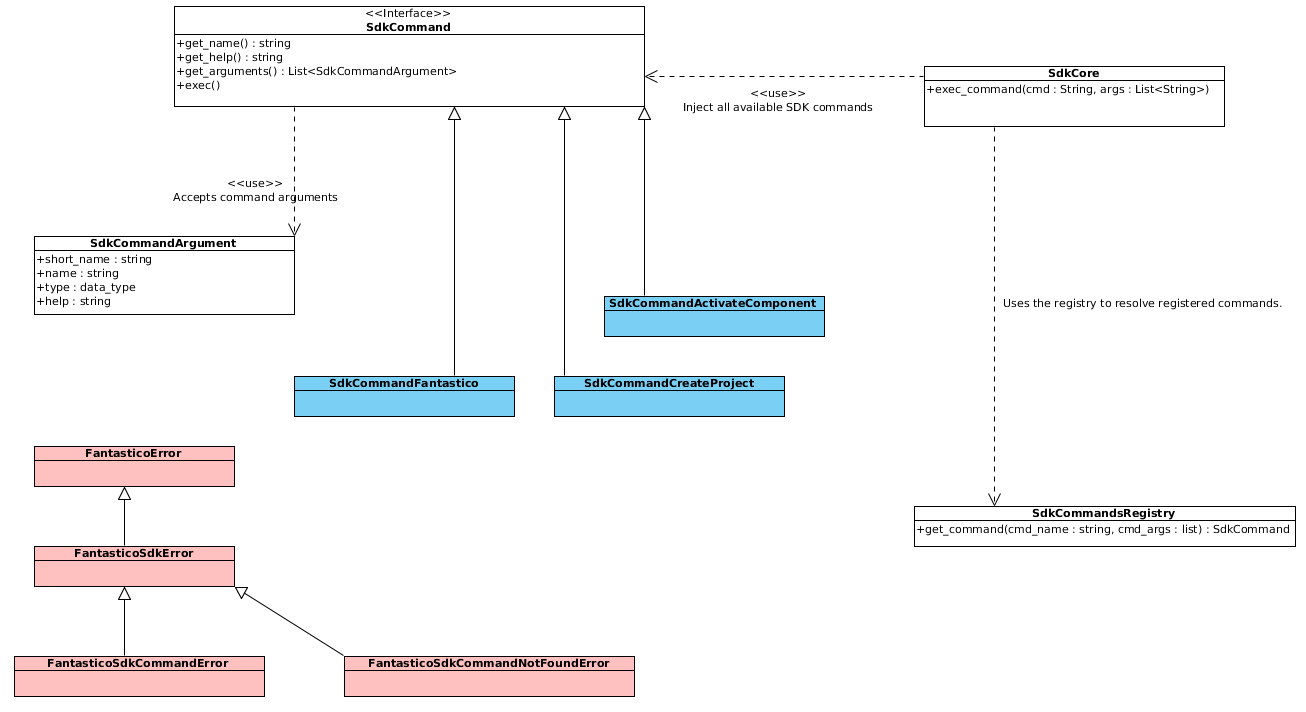
\includegraphics{design.png}

As you can see in above diagram, sdk core is just the main entry point of Fantastico Software Development Kit. It wires
all available sdk commands together and it adds support for uniformly executes them and pass them arguments..
\index{exec() (fantastico.sdk.fantastico.SdkCore method)}

\begin{fulllineitems}
\phantomsection\label{features/sdk:fantastico.sdk.fantastico.SdkCore.exec}\pysiglinewithargsret{\bfcode{exec}}{}{}
This method does nothing because fantastico is designed to accept only registered subcommands.

\end{fulllineitems}

\index{get\_arguments() (fantastico.sdk.fantastico.SdkCore method)}

\begin{fulllineitems}
\phantomsection\label{features/sdk:fantastico.sdk.fantastico.SdkCore.get_arguments}\pysiglinewithargsret{\bfcode{get\_arguments}}{}{}
This property retrieves support fantastico arguments.

\end{fulllineitems}

\index{get\_help() (fantastico.sdk.fantastico.SdkCore method)}

\begin{fulllineitems}
\phantomsection\label{features/sdk:fantastico.sdk.fantastico.SdkCore.get_help}\pysiglinewithargsret{\bfcode{get\_help}}{}{}
This method returns the friendly help message describing the method.

\end{fulllineitems}


\end{fulllineitems}

\index{SdkCommandsRegistry (class in fantastico.sdk.sdk\_core)}

\begin{fulllineitems}
\phantomsection\label{features/sdk:fantastico.sdk.sdk_core.SdkCommandsRegistry}\pysigline{\strong{class }\code{fantastico.sdk.sdk\_core.}\bfcode{SdkCommandsRegistry}}
This class holds all registered commands available to use in the sdk. It is important to understand that commands and
subcommands are registered by name and must be unique. This is because, by design, each command can easily become a
subcommand for another command. It facilitates very flexible extension of sdk and reusage of existing commands.
\index{add\_command() (fantastico.sdk.sdk\_core.SdkCommandsRegistry static method)}

\begin{fulllineitems}
\phantomsection\label{features/sdk:fantastico.sdk.sdk_core.SdkCommandsRegistry.add_command}\pysiglinewithargsret{\strong{static }\bfcode{add\_command}}{\emph{cmd\_name}, \emph{cmd\_cls}}{}
This method registers a new command using the given name.
\begin{quote}\begin{description}
\item[{Parameters}] \leavevmode\begin{itemize}
\item {} 
\textbf{cmd\_name} (\emph{str}) -- Command name used to uniquely identify the command.

\item {} 
\textbf{cmd\_class} ({\hyperref[features/sdk:fantastico.sdk.sdk_core.SdkCommand]{\code{fantastico.sdk.sdk\_core.SdkCommand}}}) -- A subclass of sdk command.

\end{itemize}

\item[{Raises {\hyperref[features/sdk:fantastico.sdk.sdk_exceptions.FantasticoSdkError]{fantastico.sdk.sdk\_exceptions.FantasticoSdkError}}}] \leavevmode
If the given name is not unique or cmd class is wrong.

\end{description}\end{quote}

\end{fulllineitems}

\index{get\_command() (fantastico.sdk.sdk\_core.SdkCommandsRegistry static method)}

\begin{fulllineitems}
\phantomsection\label{features/sdk:fantastico.sdk.sdk_core.SdkCommandsRegistry.get_command}\pysiglinewithargsret{\strong{static }\bfcode{get\_command}}{\emph{cmd\_name}, \emph{cmd\_args}}{}
This method retrieve a concrete sdk command by name with the give args passed.
\begin{quote}\begin{description}
\item[{Parameters}] \leavevmode\begin{itemize}
\item {} 
\textbf{cmd\_name} (\emph{str}) -- The registered command name we want to instantiate.

\item {} 
\textbf{cmd\_args} (\emph{list}) -- a list of arguments received from command line.

\end{itemize}

\item[{Returns}] \leavevmode
Command instance.

\item[{Return type}] \leavevmode
{\hyperref[features/sdk:fantastico.sdk.sdk_core.SdkCommand]{\code{fantastico.sdk.sdk\_core.SdkCommand}}}

\item[{Raises {\hyperref[features/sdk:fantastico.sdk.sdk_exceptions.FantasticoSdkCommandNotFoundError]{fantastico.sdk.sdk\_exceptions.FantasticoSdkCommandNotFoundError}}}] \leavevmode
if command is not registered.

\end{description}\end{quote}

\end{fulllineitems}


\end{fulllineitems}

\index{SdkCommandArgument (class in fantastico.sdk.sdk\_core)}

\begin{fulllineitems}
\phantomsection\label{features/sdk:fantastico.sdk.sdk_core.SdkCommandArgument}\pysiglinewithargsret{\strong{class }\code{fantastico.sdk.sdk\_core.}\bfcode{SdkCommandArgument}}{\emph{arg\_short\_name}, \emph{arg\_name}, \emph{arg\_type}, \emph{arg\_help}}{}
This class describe the attributes supported by a command argument. For a simple example of how arguments are used
read {\hyperref[features/sdk:fantastico.sdk.sdk_core.SdkCommand]{\code{fantastico.sdk.sdk\_core.SdkCommand}}}
\index{help (fantastico.sdk.sdk\_core.SdkCommandArgument attribute)}

\begin{fulllineitems}
\phantomsection\label{features/sdk:fantastico.sdk.sdk_core.SdkCommandArgument.help}\pysigline{\bfcode{help}}
This read only property holds the argument help message.

\end{fulllineitems}

\index{name (fantastico.sdk.sdk\_core.SdkCommandArgument attribute)}

\begin{fulllineitems}
\phantomsection\label{features/sdk:fantastico.sdk.sdk_core.SdkCommandArgument.name}\pysigline{\bfcode{name}}
This read only property holds the argument name. Name property will represent the long name argument available for
sdk commands. E.g: \textbf{--name}.

\end{fulllineitems}

\index{short\_name (fantastico.sdk.sdk\_core.SdkCommandArgument attribute)}

\begin{fulllineitems}
\phantomsection\label{features/sdk:fantastico.sdk.sdk_core.SdkCommandArgument.short_name}\pysigline{\bfcode{short\_name}}
This read only property holds the argument short name. Short name property will represent the short name argument
available for sdk commands. E.g: \textbf{-n}.

\end{fulllineitems}

\index{type (fantastico.sdk.sdk\_core.SdkCommandArgument attribute)}

\begin{fulllineitems}
\phantomsection\label{features/sdk:fantastico.sdk.sdk_core.SdkCommandArgument.type}\pysigline{\bfcode{type}}
This read only property holds the argument type.

\end{fulllineitems}


\end{fulllineitems}

\index{SdkCommand (class in fantastico.sdk.sdk\_core)}

\begin{fulllineitems}
\phantomsection\label{features/sdk:fantastico.sdk.sdk_core.SdkCommand}\pysiglinewithargsret{\strong{class }\code{fantastico.sdk.sdk\_core.}\bfcode{SdkCommand}}{\emph{argv}, \emph{cmd\_factory}}{}
This class provides the contract which must be provided by each concrete command. A command of sdk is just and extension
which can provide custom actions being executed by Fantastico in a uniform manner.

Below you can find a simple example of how to implement a concrete command:

In the previous example, we have shown that all received arguments from command line are magically provided into
\textbf{self.\_arguments} attribute of the command.

When a sdk command is instantiated with a list of command line arguments the first element from the list must be the command
name. This happens because all arguments passed after a command name belongs only to that command.
\index{exec() (fantastico.sdk.sdk\_core.SdkCommand method)}

\begin{fulllineitems}
\phantomsection\label{features/sdk:fantastico.sdk.sdk_core.SdkCommand.exec}\pysiglinewithargsret{\bfcode{exec}}{}{}
This method must be overriden by each concrete command and must provide the command execution logic.
\begin{quote}\begin{description}
\item[{Raises {\hyperref[features/sdk:fantastico.sdk.sdk_exceptions.FantasticoSdkCommandError]{fantastico.sdk.sdk\_exceptions.FantasticoSdkCommandError}}}] \leavevmode
if an exception occurs while executing the command.

\end{description}\end{quote}

\end{fulllineitems}

\index{exec\_command() (fantastico.sdk.sdk\_core.SdkCommand method)}

\begin{fulllineitems}
\phantomsection\label{features/sdk:fantastico.sdk.sdk_core.SdkCommand.exec_command}\pysiglinewithargsret{\bfcode{exec\_command}}{\emph{*args}, \emph{**kwargs}}{}
This method provides a template for executing the current command if subcommands are present. Internally it invokes
overriden exec method.
\begin{quote}\begin{description}
\item[{Raises}] \leavevmode\begin{itemize}
\item {} 
{\hyperref[features/sdk:fantastico.sdk.sdk_exceptions.FantasticoSdkCommandError]{\textbf{fantastico.sdk.sdk\_exceptions.FantasticoSdkCommandError}}} -- if an exception occurs while executing the command.

\item {} 
{\hyperref[features/sdk:fantastico.sdk.sdk_exceptions.FantasticoSdkCommandNotFoundError]{\textbf{fantastico.sdk.sdk\_exceptions.FantasticoSdkCommandNotFoundError}}} -- if a subcommand does not exist.

\end{itemize}

\end{description}\end{quote}

\end{fulllineitems}

\index{get\_arguments() (fantastico.sdk.sdk\_core.SdkCommand method)}

\begin{fulllineitems}
\phantomsection\label{features/sdk:fantastico.sdk.sdk_core.SdkCommand.get_arguments}\pysiglinewithargsret{\bfcode{get\_arguments}}{}{}
This method must be overriden by each concrete command and must return the command supported arguments.

\end{fulllineitems}


\end{fulllineitems}

\index{SdkCommand (class in fantastico.sdk.sdk\_decorators)}

\begin{fulllineitems}
\phantomsection\label{features/sdk:fantastico.sdk.sdk_decorators.SdkCommand}\pysiglinewithargsret{\strong{class }\code{fantastico.sdk.sdk\_decorators.}\bfcode{SdkCommand}}{\emph{name}, \emph{help}, \emph{target=None}, \emph{settings\_facade\_cls=\textless{}class `fantastico.settings.SettingsFacade'\textgreater{}}}{}
This decorator describe the sdk commands metadata:
\begin{enumerate}
\item {} 
name

\item {} 
target (which is the main purpose of the command. E.g: fantastico - this mean command is designed to work as a subcommand for fantastico cmd).

\item {} 
help (which describes what this method does). It will automatically contain a link to official fantastico documentation of the command.

\end{enumerate}

It is used in conjunction with {\hyperref[features/sdk:fantastico.sdk.sdk_core.SdkCommand]{\code{fantastico.sdk.sdk\_core.SdkCommand}}}. Each sdk command decorated with this
decorator automatically receives \textbf{get\_name} and \textbf{get\_target} methods.

\end{fulllineitems}

\index{FantasticoSdkError (class in fantastico.sdk.sdk\_exceptions)}

\begin{fulllineitems}
\phantomsection\label{features/sdk:fantastico.sdk.sdk_exceptions.FantasticoSdkError}\pysiglinewithargsret{\strong{class }\code{fantastico.sdk.sdk\_exceptions.}\bfcode{FantasticoSdkError}}{\emph{msg=None}, \emph{http\_code=400}}{}
This is the base exception used to describe unexpected situations occuring into fantastico sdk. Below you can see the
sdk hierarchy of concrete exceptions.

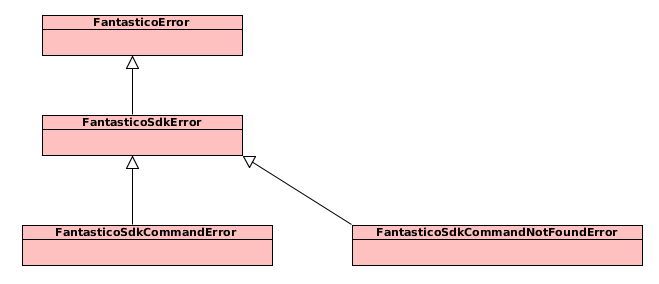
\includegraphics{exceptions1.png}

\end{fulllineitems}

\index{FantasticoSdkCommandError (class in fantastico.sdk.sdk\_exceptions)}

\begin{fulllineitems}
\phantomsection\label{features/sdk:fantastico.sdk.sdk_exceptions.FantasticoSdkCommandError}\pysiglinewithargsret{\strong{class }\code{fantastico.sdk.sdk\_exceptions.}\bfcode{FantasticoSdkCommandError}}{\emph{msg=None}, \emph{http\_code=400}}{}
This class describe an exception which occured into one of fantastico sdk commands.

\end{fulllineitems}

\index{FantasticoSdkCommandNotFoundError (class in fantastico.sdk.sdk\_exceptions)}

\begin{fulllineitems}
\phantomsection\label{features/sdk:fantastico.sdk.sdk_exceptions.FantasticoSdkCommandNotFoundError}\pysiglinewithargsret{\strong{class }\code{fantastico.sdk.sdk\_exceptions.}\bfcode{FantasticoSdkCommandNotFoundError}}{\emph{msg=None}, \emph{http\_code=400}}{}
This class describe an exception which occurs when we try to execute an inexistent command.

\end{fulllineitems}



\section{Component model}
\label{features/component_model::doc}\label{features/component_model:component-model}
In Fantastico there is no enforced component model for your code but there are a set of recommendations
that will make your life a lot easier when organizing projects. A typical \textbf{component} structure looks like:
\begin{itemize}
\item {} \begin{description}
\item[{\textless{}your project folder\textgreater{}}] \leavevmode\begin{itemize}
\item {} \begin{description}
\item[{component\_1}] \leavevmode\begin{itemize}
\item {} 
models (sql alchemy models)

\item {} 
static (static files holder)

\item {} 
views (all views used by this component controllers')

\item {} 
sql (sql scripts required to setup the component)

\item {} 
\_\_init\_\_.py

\item {} 
*.py (controller module files)

\end{itemize}

\end{description}

\end{itemize}

\end{description}

\end{itemize}

You can usually structure your code as you want, but Fantastico default {\hyperref[features/mvc::doc]{\emph{Model View Controller}}} registrators are assuming
component name is the parent folder of the controller module. This is why is best to follow the above mentioned structure.
None of the above folders are mandatory which gives you, developer, plenty of flexibility but also responsibility. For
more information about \textbf{models}, \textbf{views} and \textbf{controllers} read {\hyperref[how_to/mvc_how_to::doc]{\emph{MVC How to}}} section.


\subsection{Static folder}
\label{features/component_model:static-folder}
By default, static folder holds all static assets belonging to a component. You can find more information about this
in {\hyperref[how_to/static_assets::doc]{\emph{Static assets}}} section.


\subsection{Sql folder}
\label{features/component_model:sql-folder}
Sql folder is used to hold all sql scripts required for a component to work correctly. In our continuous delivery
process we scan all available sql folders and execute \textbf{module\_setup.sql} scripts. By default, we want to give
developers the chance to provide a setup script for each component in order to easily install the component database
dependencies.

For easily synchronization of sql scripts with a \textbf{Fantastico} project database read {\hyperref[features/sdk/command_syncdb::doc]{\emph{Syncdb command}}}


\subsubsection{Sql folder example}
\label{features/component_model:sql-folder-example}
Assume you want to create a blog module that requires a storage for \textbf{Authors} and \textbf{Posts}. module\_setup.sql script
is the perfect place to provide the code. We recommend to make this code idempotent, meaning that once dependencies are
created they should not be altered anymore by this script.

An example of such a script we use in integration tests can be found under: \textbf{/\textless{}fantastico\_framework\textgreater{}/samples/mvc/sql/module\_setup.sql}.

\begin{Verbatim}[commandchars=\\\{\}]
\PYG{o}{\PYGZsh{}}\PYG{o}{\PYGZsh{}}\PYG{o}{\PYGZsh{}}\PYG{o}{\PYGZsh{}}\PYG{o}{\PYGZsh{}}\PYG{o}{\PYGZsh{}}\PYG{o}{\PYGZsh{}}\PYG{o}{\PYGZsh{}}\PYG{o}{\PYGZsh{}}\PYG{o}{\PYGZsh{}}\PYG{o}{\PYGZsh{}}\PYG{o}{\PYGZsh{}}\PYG{o}{\PYGZsh{}}\PYG{o}{\PYGZsh{}}\PYG{o}{\PYGZsh{}}\PYG{o}{\PYGZsh{}}\PYG{o}{\PYGZsh{}}\PYG{o}{\PYGZsh{}}\PYG{o}{\PYGZsh{}}\PYG{o}{\PYGZsh{}}\PYG{o}{\PYGZsh{}}\PYG{o}{\PYGZsh{}}\PYG{o}{\PYGZsh{}}\PYG{o}{\PYGZsh{}}\PYG{o}{\PYGZsh{}}\PYG{o}{\PYGZsh{}}\PYG{o}{\PYGZsh{}}\PYG{o}{\PYGZsh{}}\PYG{o}{\PYGZsh{}}\PYG{o}{\PYGZsh{}}\PYG{o}{\PYGZsh{}}\PYG{o}{\PYGZsh{}}\PYG{o}{\PYGZsh{}}\PYG{o}{\PYGZsh{}}\PYG{o}{\PYGZsh{}}\PYG{o}{\PYGZsh{}}\PYG{o}{\PYGZsh{}}\PYG{o}{\PYGZsh{}}\PYG{o}{\PYGZsh{}}\PYG{o}{\PYGZsh{}}\PYG{o}{\PYGZsh{}}\PYG{o}{\PYGZsh{}}\PYG{o}{\PYGZsh{}}\PYG{o}{\PYGZsh{}}\PYG{o}{\PYGZsh{}}\PYG{o}{\PYGZsh{}}\PYG{o}{\PYGZsh{}}\PYG{o}{\PYGZsh{}}\PYG{o}{\PYGZsh{}}\PYG{o}{\PYGZsh{}}\PYG{o}{\PYGZsh{}}\PYG{o}{\PYGZsh{}}\PYG{o}{\PYGZsh{}}\PYG{o}{\PYGZsh{}}\PYG{o}{\PYGZsh{}}\PYG{o}{\PYGZsh{}}\PYG{o}{\PYGZsh{}}\PYG{o}{\PYGZsh{}}\PYG{o}{\PYGZsh{}}\PYG{o}{\PYGZsh{}}\PYG{o}{\PYGZsh{}}\PYG{o}{\PYGZsh{}}\PYG{o}{\PYGZsh{}}\PYG{o}{\PYGZsh{}}\PYG{o}{\PYGZsh{}}\PYG{o}{\PYGZsh{}}\PYG{o}{\PYGZsh{}}\PYG{o}{\PYGZsh{}}\PYG{o}{\PYGZsh{}}\PYG{o}{\PYGZsh{}}\PYG{o}{\PYGZsh{}}\PYG{o}{\PYGZsh{}}\PYG{o}{\PYGZsh{}}\PYG{o}{\PYGZsh{}}\PYG{o}{\PYGZsh{}}\PYG{o}{\PYGZsh{}}\PYG{o}{\PYGZsh{}}\PYG{o}{\PYGZsh{}}\PYG{o}{\PYGZsh{}}\PYG{o}{\PYGZsh{}}\PYG{o}{\PYGZsh{}}\PYG{o}{\PYGZsh{}}\PYG{o}{\PYGZsh{}}\PYG{o}{\PYGZsh{}}\PYG{o}{\PYGZsh{}}\PYG{o}{\PYGZsh{}}\PYG{o}{\PYGZsh{}}\PYG{o}{\PYGZsh{}}\PYG{o}{\PYGZsh{}}\PYG{o}{\PYGZsh{}}\PYG{o}{\PYGZsh{}}\PYG{o}{\PYGZsh{}}\PYG{o}{\PYGZsh{}}\PYG{o}{\PYGZsh{}}\PYG{o}{\PYGZsh{}}
\PYG{o}{\PYGZsh{}} \PYG{n}{Copyright} \PYG{l+m+mi}{2013} \PYG{n}{Cosnita} \PYG{n}{Radu} \PYG{n}{Viorel}
\PYG{o}{\PYGZsh{}}
\PYG{o}{\PYGZsh{}} \PYG{n}{Permission} \PYG{k}{is} \PYG{n}{hereby} \PYG{k}{granted}\PYG{p}{,} \PYG{k}{free} \PYG{k}{of} \PYG{n}{charge}\PYG{p}{,} \PYG{k}{to} \PYG{k}{any} \PYG{n}{person} \PYG{n}{obtaining} \PYG{n}{a} \PYG{k}{copy} \PYG{k}{of} \PYG{n}{this} \PYG{n}{software}
\PYG{o}{\PYGZsh{}} \PYG{k}{and} \PYG{n}{associated} \PYG{n}{documentation} \PYG{n}{files} \PYG{p}{(}\PYG{n}{the} \PYG{l+s+ss}{\PYGZdq{}Software\PYGZdq{}}\PYG{p}{)}\PYG{p}{,} \PYG{k}{to} \PYG{n}{deal} \PYG{k}{in} \PYG{n}{the} \PYG{n}{Software} \PYG{k}{without}
\PYG{o}{\PYGZsh{}} \PYG{n}{restriction}\PYG{p}{,} \PYG{k}{including} \PYG{k}{without} \PYG{n}{limitation} \PYG{n}{the} \PYG{n}{rights} \PYG{k}{to} \PYG{n}{use}\PYG{p}{,} \PYG{k}{copy}\PYG{p}{,} \PYG{k}{modify}\PYG{p}{,} \PYG{n}{merge}\PYG{p}{,} \PYG{n}{publish}\PYG{p}{,}
\PYG{o}{\PYGZsh{}} \PYG{n}{distribute}\PYG{p}{,} \PYG{n}{sublicense}\PYG{p}{,} \PYG{k}{and}\PYG{o}{/}\PYG{k}{or} \PYG{n}{sell} \PYG{n}{copies} \PYG{k}{of} \PYG{n}{the} \PYG{n}{Software}\PYG{p}{,} \PYG{k}{and} \PYG{k}{to} \PYG{n}{permit} \PYG{n}{persons} \PYG{k}{to} \PYG{n}{whom}
\PYG{o}{\PYGZsh{}} \PYG{n}{the} \PYG{n}{Software} \PYG{k}{is} \PYG{n}{furnished} \PYG{k}{to} \PYG{k}{do} \PYG{n}{so}\PYG{p}{,} \PYG{n}{subject} \PYG{k}{to} \PYG{n}{the} \PYG{n}{following} \PYG{n}{conditions}\PYG{p}{:}
\PYG{o}{\PYGZsh{}}
\PYG{o}{\PYGZsh{}} \PYG{n}{The} \PYG{n}{above} \PYG{n}{copyright} \PYG{n}{notice} \PYG{k}{and} \PYG{n}{this} \PYG{n}{permission} \PYG{n}{notice} \PYG{n}{shall} \PYG{n}{be} \PYG{n}{included} \PYG{k}{in} \PYG{k}{all} \PYG{n}{copies} \PYG{k}{or}
\PYG{o}{\PYGZsh{}} \PYG{n}{substantial} \PYG{n}{portions} \PYG{k}{of} \PYG{n}{the} \PYG{n}{Software}\PYG{p}{.}
\PYG{o}{\PYGZsh{}}
\PYG{o}{\PYGZsh{}} \PYG{n}{THE} \PYG{n}{SOFTWARE} \PYG{k}{IS} \PYG{n}{PROVIDED} \PYG{l+s+ss}{\PYGZdq{}AS IS\PYGZdq{}}\PYG{p}{,} \PYG{k}{WITHOUT} \PYG{n}{WARRANTY} \PYG{k}{OF} \PYG{k}{ANY} \PYG{n}{KIND}\PYG{p}{,} \PYG{n}{EXPRESS} \PYG{k}{OR} \PYG{n}{IMPLIED}\PYG{p}{,}
\PYG{o}{\PYGZsh{}} \PYG{k}{INCLUDING} \PYG{n}{BUT} \PYG{k}{NOT} \PYG{n}{LIMITED} \PYG{k}{TO} \PYG{n}{THE} \PYG{n}{WARRANTIES} \PYG{k}{OF} \PYG{n}{MERCHANTABILITY}\PYG{p}{,} \PYG{n}{FITNESS} \PYG{k}{FOR} \PYG{n}{A} \PYG{n}{PARTICULAR}
\PYG{o}{\PYGZsh{}} \PYG{n}{PURPOSE} \PYG{k}{AND} \PYG{n}{NONINFRINGEMENT}\PYG{p}{.} \PYG{k}{IN} \PYG{k}{NO} \PYG{n}{EVENT} \PYG{n}{SHALL} \PYG{n}{THE} \PYG{n}{AUTHORS} \PYG{k}{OR} \PYG{n}{COPYRIGHT} \PYG{n}{HOLDERS} \PYG{n}{BE} \PYG{n}{LIABLE} \PYG{k}{FOR}
\PYG{o}{\PYGZsh{}} \PYG{k}{ANY} \PYG{n}{CLAIM}\PYG{p}{,} \PYG{n}{DAMAGES} \PYG{k}{OR} \PYG{n}{OTHER} \PYG{n}{LIABILITY}\PYG{p}{,} \PYG{n}{WHETHER} \PYG{k}{IN} \PYG{n}{AN} \PYG{n}{ACTION} \PYG{k}{OF} \PYG{n}{CONTRACT}\PYG{p}{,} \PYG{n}{TORT} \PYG{k}{OR} \PYG{n}{OTHERWISE}\PYG{p}{,}
\PYG{o}{\PYGZsh{}} \PYG{n}{ARISING} \PYG{k}{FROM}\PYG{p}{,} \PYG{k}{OUT} \PYG{k}{OF} \PYG{k}{OR} \PYG{k}{IN} \PYG{k}{CONNECTION} \PYG{k}{WITH} \PYG{n}{THE} \PYG{n}{SOFTWARE} \PYG{k}{OR} \PYG{n}{THE} \PYG{n}{USE} \PYG{k}{OR} \PYG{n}{OTHER} \PYG{n}{DEALINGS}
\PYG{o}{\PYGZsh{}} \PYG{k}{IN} \PYG{n}{THE} \PYG{n}{SOFTWARE}\PYG{p}{.}
\PYG{o}{\PYGZsh{}}\PYG{o}{\PYGZsh{}}\PYG{o}{\PYGZsh{}}\PYG{o}{\PYGZsh{}}\PYG{o}{\PYGZsh{}}\PYG{o}{\PYGZsh{}}\PYG{o}{\PYGZsh{}}\PYG{o}{\PYGZsh{}}\PYG{o}{\PYGZsh{}}\PYG{o}{\PYGZsh{}}\PYG{o}{\PYGZsh{}}\PYG{o}{\PYGZsh{}}\PYG{o}{\PYGZsh{}}\PYG{o}{\PYGZsh{}}\PYG{o}{\PYGZsh{}}\PYG{o}{\PYGZsh{}}\PYG{o}{\PYGZsh{}}\PYG{o}{\PYGZsh{}}\PYG{o}{\PYGZsh{}}\PYG{o}{\PYGZsh{}}\PYG{o}{\PYGZsh{}}\PYG{o}{\PYGZsh{}}\PYG{o}{\PYGZsh{}}\PYG{o}{\PYGZsh{}}\PYG{o}{\PYGZsh{}}\PYG{o}{\PYGZsh{}}\PYG{o}{\PYGZsh{}}\PYG{o}{\PYGZsh{}}\PYG{o}{\PYGZsh{}}\PYG{o}{\PYGZsh{}}\PYG{o}{\PYGZsh{}}\PYG{o}{\PYGZsh{}}\PYG{o}{\PYGZsh{}}\PYG{o}{\PYGZsh{}}\PYG{o}{\PYGZsh{}}\PYG{o}{\PYGZsh{}}\PYG{o}{\PYGZsh{}}\PYG{o}{\PYGZsh{}}\PYG{o}{\PYGZsh{}}\PYG{o}{\PYGZsh{}}\PYG{o}{\PYGZsh{}}\PYG{o}{\PYGZsh{}}\PYG{o}{\PYGZsh{}}\PYG{o}{\PYGZsh{}}\PYG{o}{\PYGZsh{}}\PYG{o}{\PYGZsh{}}\PYG{o}{\PYGZsh{}}\PYG{o}{\PYGZsh{}}\PYG{o}{\PYGZsh{}}\PYG{o}{\PYGZsh{}}\PYG{o}{\PYGZsh{}}\PYG{o}{\PYGZsh{}}\PYG{o}{\PYGZsh{}}\PYG{o}{\PYGZsh{}}\PYG{o}{\PYGZsh{}}\PYG{o}{\PYGZsh{}}\PYG{o}{\PYGZsh{}}\PYG{o}{\PYGZsh{}}\PYG{o}{\PYGZsh{}}\PYG{o}{\PYGZsh{}}\PYG{o}{\PYGZsh{}}\PYG{o}{\PYGZsh{}}\PYG{o}{\PYGZsh{}}\PYG{o}{\PYGZsh{}}\PYG{o}{\PYGZsh{}}\PYG{o}{\PYGZsh{}}\PYG{o}{\PYGZsh{}}\PYG{o}{\PYGZsh{}}\PYG{o}{\PYGZsh{}}\PYG{o}{\PYGZsh{}}\PYG{o}{\PYGZsh{}}\PYG{o}{\PYGZsh{}}\PYG{o}{\PYGZsh{}}\PYG{o}{\PYGZsh{}}\PYG{o}{\PYGZsh{}}\PYG{o}{\PYGZsh{}}\PYG{o}{\PYGZsh{}}\PYG{o}{\PYGZsh{}}\PYG{o}{\PYGZsh{}}\PYG{o}{\PYGZsh{}}\PYG{o}{\PYGZsh{}}\PYG{o}{\PYGZsh{}}\PYG{o}{\PYGZsh{}}\PYG{o}{\PYGZsh{}}\PYG{o}{\PYGZsh{}}\PYG{o}{\PYGZsh{}}\PYG{o}{\PYGZsh{}}\PYG{o}{\PYGZsh{}}\PYG{o}{\PYGZsh{}}\PYG{o}{\PYGZsh{}}\PYG{o}{\PYGZsh{}}\PYG{o}{\PYGZsh{}}\PYG{o}{\PYGZsh{}}\PYG{o}{\PYGZsh{}}\PYG{o}{\PYGZsh{}}


\PYG{k}{DROP} \PYG{k}{TABLE} \PYG{n}{IF} \PYG{k}{EXISTS} \PYG{n}{mvc\PYGZus{}friendly\PYGZus{}messages}\PYG{p}{;}
\PYG{k}{CREATE} \PYG{k}{TABLE} \PYG{n}{mvc\PYGZus{}friendly\PYGZus{}messages}\PYG{p}{(}
   \PYG{n}{Id} \PYG{n+nb}{INT} \PYG{n}{AUTO\PYGZus{}INCREMENT}\PYG{p}{,}
   \PYG{n}{Message} \PYG{n+nb}{TEXT}\PYG{p}{,}
   \PYG{k}{PRIMARY} \PYG{k}{KEY}\PYG{p}{(}\PYG{n}{id}\PYG{p}{)}\PYG{p}{)}\PYG{p}{;}
\end{Verbatim}

Once the component is activated ({\hyperref[features/sdk/command_activate_extension::doc]{\emph{Activate extension command}}}) and structure is synchronize data must be
created into the new tables. You can find such a script example below. It is up to you where you place \textbf{sql/create\_data.sql}.

\begin{Verbatim}[commandchars=\\\{\}]
\PYG{o}{\PYGZsh{}}\PYG{o}{\PYGZsh{}}\PYG{o}{\PYGZsh{}}\PYG{o}{\PYGZsh{}}\PYG{o}{\PYGZsh{}}\PYG{o}{\PYGZsh{}}\PYG{o}{\PYGZsh{}}\PYG{o}{\PYGZsh{}}\PYG{o}{\PYGZsh{}}\PYG{o}{\PYGZsh{}}\PYG{o}{\PYGZsh{}}\PYG{o}{\PYGZsh{}}\PYG{o}{\PYGZsh{}}\PYG{o}{\PYGZsh{}}\PYG{o}{\PYGZsh{}}\PYG{o}{\PYGZsh{}}\PYG{o}{\PYGZsh{}}\PYG{o}{\PYGZsh{}}\PYG{o}{\PYGZsh{}}\PYG{o}{\PYGZsh{}}\PYG{o}{\PYGZsh{}}\PYG{o}{\PYGZsh{}}\PYG{o}{\PYGZsh{}}\PYG{o}{\PYGZsh{}}\PYG{o}{\PYGZsh{}}\PYG{o}{\PYGZsh{}}\PYG{o}{\PYGZsh{}}\PYG{o}{\PYGZsh{}}\PYG{o}{\PYGZsh{}}\PYG{o}{\PYGZsh{}}\PYG{o}{\PYGZsh{}}\PYG{o}{\PYGZsh{}}\PYG{o}{\PYGZsh{}}\PYG{o}{\PYGZsh{}}\PYG{o}{\PYGZsh{}}\PYG{o}{\PYGZsh{}}\PYG{o}{\PYGZsh{}}\PYG{o}{\PYGZsh{}}\PYG{o}{\PYGZsh{}}\PYG{o}{\PYGZsh{}}\PYG{o}{\PYGZsh{}}\PYG{o}{\PYGZsh{}}\PYG{o}{\PYGZsh{}}\PYG{o}{\PYGZsh{}}\PYG{o}{\PYGZsh{}}\PYG{o}{\PYGZsh{}}\PYG{o}{\PYGZsh{}}\PYG{o}{\PYGZsh{}}\PYG{o}{\PYGZsh{}}\PYG{o}{\PYGZsh{}}\PYG{o}{\PYGZsh{}}\PYG{o}{\PYGZsh{}}\PYG{o}{\PYGZsh{}}\PYG{o}{\PYGZsh{}}\PYG{o}{\PYGZsh{}}\PYG{o}{\PYGZsh{}}\PYG{o}{\PYGZsh{}}\PYG{o}{\PYGZsh{}}\PYG{o}{\PYGZsh{}}\PYG{o}{\PYGZsh{}}\PYG{o}{\PYGZsh{}}\PYG{o}{\PYGZsh{}}\PYG{o}{\PYGZsh{}}\PYG{o}{\PYGZsh{}}\PYG{o}{\PYGZsh{}}\PYG{o}{\PYGZsh{}}\PYG{o}{\PYGZsh{}}\PYG{o}{\PYGZsh{}}\PYG{o}{\PYGZsh{}}\PYG{o}{\PYGZsh{}}\PYG{o}{\PYGZsh{}}\PYG{o}{\PYGZsh{}}\PYG{o}{\PYGZsh{}}\PYG{o}{\PYGZsh{}}\PYG{o}{\PYGZsh{}}\PYG{o}{\PYGZsh{}}\PYG{o}{\PYGZsh{}}\PYG{o}{\PYGZsh{}}\PYG{o}{\PYGZsh{}}\PYG{o}{\PYGZsh{}}\PYG{o}{\PYGZsh{}}\PYG{o}{\PYGZsh{}}\PYG{o}{\PYGZsh{}}\PYG{o}{\PYGZsh{}}\PYG{o}{\PYGZsh{}}\PYG{o}{\PYGZsh{}}\PYG{o}{\PYGZsh{}}\PYG{o}{\PYGZsh{}}\PYG{o}{\PYGZsh{}}\PYG{o}{\PYGZsh{}}\PYG{o}{\PYGZsh{}}\PYG{o}{\PYGZsh{}}\PYG{o}{\PYGZsh{}}\PYG{o}{\PYGZsh{}}\PYG{o}{\PYGZsh{}}\PYG{o}{\PYGZsh{}}\PYG{o}{\PYGZsh{}}\PYG{o}{\PYGZsh{}}\PYG{o}{\PYGZsh{}}\PYG{o}{\PYGZsh{}}\PYG{o}{\PYGZsh{}}\PYG{o}{\PYGZsh{}}\PYG{o}{\PYGZsh{}}\PYG{o}{\PYGZsh{}}\PYG{o}{\PYGZsh{}}\PYG{o}{\PYGZsh{}}\PYG{o}{\PYGZsh{}}\PYG{o}{\PYGZsh{}}\PYG{o}{\PYGZsh{}}\PYG{o}{\PYGZsh{}}\PYG{o}{\PYGZsh{}}\PYG{o}{\PYGZsh{}}\PYG{o}{\PYGZsh{}}\PYG{o}{\PYGZsh{}}\PYG{o}{\PYGZsh{}}\PYG{o}{\PYGZsh{}}\PYG{o}{\PYGZsh{}}\PYG{o}{\PYGZsh{}}\PYG{o}{\PYGZsh{}}\PYG{o}{\PYGZsh{}}\PYG{o}{\PYGZsh{}}\PYG{o}{\PYGZsh{}}\PYG{o}{\PYGZsh{}}\PYG{o}{\PYGZsh{}}\PYG{o}{\PYGZsh{}}\PYG{o}{\PYGZsh{}}
\PYG{o}{\PYGZsh{}} \PYG{n}{Copyright} \PYG{l+m+mi}{2013} \PYG{n}{Cosnita} \PYG{n}{Radu} \PYG{n}{Viorel}
\PYG{o}{\PYGZsh{}}
\PYG{o}{\PYGZsh{}} \PYG{n}{Permission} \PYG{k}{is} \PYG{n}{hereby} \PYG{k}{granted}\PYG{p}{,} \PYG{k}{free} \PYG{k}{of} \PYG{n}{charge}\PYG{p}{,} \PYG{k}{to} \PYG{k}{any} \PYG{n}{person} \PYG{n}{obtaining} \PYG{n}{a} \PYG{k}{copy} \PYG{k}{of} \PYG{n}{this} \PYG{n}{software} \PYG{k}{and} \PYG{n}{associated}
\PYG{o}{\PYGZsh{}} \PYG{n}{documentation} \PYG{n}{files} \PYG{p}{(}\PYG{n}{the} \PYG{l+s+ss}{\PYGZdq{}Software\PYGZdq{}}\PYG{p}{)}\PYG{p}{,} \PYG{k}{to} \PYG{n}{deal} \PYG{k}{in} \PYG{n}{the} \PYG{n}{Software} \PYG{k}{without} \PYG{n}{restriction}\PYG{p}{,} \PYG{k}{including} \PYG{k}{without} \PYG{n}{limitation}
\PYG{o}{\PYGZsh{}} \PYG{n}{the} \PYG{n}{rights} \PYG{k}{to} \PYG{n}{use}\PYG{p}{,} \PYG{k}{copy}\PYG{p}{,} \PYG{k}{modify}\PYG{p}{,} \PYG{n}{merge}\PYG{p}{,} \PYG{n}{publish}\PYG{p}{,} \PYG{n}{distribute}\PYG{p}{,} \PYG{n}{sublicense}\PYG{p}{,} \PYG{k}{and}\PYG{o}{/}\PYG{k}{or} \PYG{n}{sell} \PYG{n}{copies} \PYG{k}{of} \PYG{n}{the} \PYG{n}{Software}\PYG{p}{,}
\PYG{o}{\PYGZsh{}} \PYG{k}{and} \PYG{k}{to} \PYG{n}{permit} \PYG{n}{persons} \PYG{k}{to} \PYG{n}{whom} \PYG{n}{the} \PYG{n}{Software} \PYG{k}{is} \PYG{n}{furnished} \PYG{k}{to} \PYG{k}{do} \PYG{n}{so}\PYG{p}{,} \PYG{n}{subject} \PYG{k}{to} \PYG{n}{the} \PYG{n}{following} \PYG{n}{conditions}\PYG{p}{:}
\PYG{o}{\PYGZsh{}}
\PYG{o}{\PYGZsh{}} \PYG{n}{The} \PYG{n}{above} \PYG{n}{copyright} \PYG{n}{notice} \PYG{k}{and} \PYG{n}{this} \PYG{n}{permission} \PYG{n}{notice} \PYG{n}{shall} \PYG{n}{be} \PYG{n}{included} \PYG{k}{in} \PYG{k}{all} \PYG{n}{copies} \PYG{k}{or} \PYG{n}{substantial} \PYG{n}{portions} \PYG{k}{of} \PYG{n}{the} \PYG{n}{Software}\PYG{p}{.}
\PYG{o}{\PYGZsh{}}
\PYG{o}{\PYGZsh{}} \PYG{n}{THE} \PYG{n}{SOFTWARE} \PYG{k}{IS} \PYG{n}{PROVIDED} \PYG{l+s+ss}{\PYGZdq{}AS IS\PYGZdq{}}\PYG{p}{,} \PYG{k}{WITHOUT} \PYG{n}{WARRANTY} \PYG{k}{OF} \PYG{k}{ANY} \PYG{n}{KIND}\PYG{p}{,} \PYG{n}{EXPRESS} \PYG{k}{OR} \PYG{n}{IMPLIED}\PYG{p}{,} \PYG{k}{INCLUDING} \PYG{n}{BUT} \PYG{k}{NOT} \PYG{n}{LIMITED} \PYG{k}{TO} \PYG{n}{THE}
\PYG{o}{\PYGZsh{}} \PYG{n}{WARRANTIES} \PYG{k}{OF} \PYG{n}{MERCHANTABILITY}\PYG{p}{,} \PYG{n}{FITNESS} \PYG{k}{FOR} \PYG{n}{A} \PYG{n}{PARTICULAR} \PYG{n}{PURPOSE} \PYG{k}{AND} \PYG{n}{NONINFRINGEMENT}\PYG{p}{.} \PYG{k}{IN} \PYG{k}{NO} \PYG{n}{EVENT} \PYG{n}{SHALL} \PYG{n}{THE} \PYG{n}{AUTHORS} \PYG{k}{OR}
\PYG{o}{\PYGZsh{}} \PYG{n}{COPYRIGHT} \PYG{n}{HOLDERS} \PYG{n}{BE} \PYG{n}{LIABLE} \PYG{k}{FOR} \PYG{k}{ANY} \PYG{n}{CLAIM}\PYG{p}{,} \PYG{n}{DAMAGES} \PYG{k}{OR} \PYG{n}{OTHER} \PYG{n}{LIABILITY}\PYG{p}{,} \PYG{n}{WHETHER} \PYG{k}{IN} \PYG{n}{AN} \PYG{n}{ACTION} \PYG{k}{OF} \PYG{n}{CONTRACT}\PYG{p}{,} \PYG{n}{TORT} \PYG{k}{OR} \PYG{n}{OTHERWISE}\PYG{p}{,}
\PYG{o}{\PYGZsh{}} \PYG{n}{ARISING} \PYG{k}{FROM}\PYG{p}{,} \PYG{k}{OUT} \PYG{k}{OF} \PYG{k}{OR} \PYG{k}{IN} \PYG{k}{CONNECTION} \PYG{k}{WITH} \PYG{n}{THE} \PYG{n}{SOFTWARE} \PYG{k}{OR} \PYG{n}{THE} \PYG{n}{USE} \PYG{k}{OR} \PYG{n}{OTHER} \PYG{n}{DEALINGS} \PYG{k}{IN} \PYG{n}{THE} \PYG{n}{SOFTWARE}\PYG{p}{.}
\PYG{o}{\PYGZsh{}}\PYG{o}{\PYGZsh{}}\PYG{o}{\PYGZsh{}}\PYG{o}{\PYGZsh{}}\PYG{o}{\PYGZsh{}}\PYG{o}{\PYGZsh{}}\PYG{o}{\PYGZsh{}}\PYG{o}{\PYGZsh{}}\PYG{o}{\PYGZsh{}}\PYG{o}{\PYGZsh{}}\PYG{o}{\PYGZsh{}}\PYG{o}{\PYGZsh{}}\PYG{o}{\PYGZsh{}}\PYG{o}{\PYGZsh{}}\PYG{o}{\PYGZsh{}}\PYG{o}{\PYGZsh{}}\PYG{o}{\PYGZsh{}}\PYG{o}{\PYGZsh{}}\PYG{o}{\PYGZsh{}}\PYG{o}{\PYGZsh{}}\PYG{o}{\PYGZsh{}}\PYG{o}{\PYGZsh{}}\PYG{o}{\PYGZsh{}}\PYG{o}{\PYGZsh{}}\PYG{o}{\PYGZsh{}}\PYG{o}{\PYGZsh{}}\PYG{o}{\PYGZsh{}}\PYG{o}{\PYGZsh{}}\PYG{o}{\PYGZsh{}}\PYG{o}{\PYGZsh{}}\PYG{o}{\PYGZsh{}}\PYG{o}{\PYGZsh{}}\PYG{o}{\PYGZsh{}}\PYG{o}{\PYGZsh{}}\PYG{o}{\PYGZsh{}}\PYG{o}{\PYGZsh{}}\PYG{o}{\PYGZsh{}}\PYG{o}{\PYGZsh{}}\PYG{o}{\PYGZsh{}}\PYG{o}{\PYGZsh{}}\PYG{o}{\PYGZsh{}}\PYG{o}{\PYGZsh{}}\PYG{o}{\PYGZsh{}}\PYG{o}{\PYGZsh{}}\PYG{o}{\PYGZsh{}}\PYG{o}{\PYGZsh{}}\PYG{o}{\PYGZsh{}}\PYG{o}{\PYGZsh{}}\PYG{o}{\PYGZsh{}}\PYG{o}{\PYGZsh{}}\PYG{o}{\PYGZsh{}}\PYG{o}{\PYGZsh{}}\PYG{o}{\PYGZsh{}}\PYG{o}{\PYGZsh{}}\PYG{o}{\PYGZsh{}}\PYG{o}{\PYGZsh{}}\PYG{o}{\PYGZsh{}}\PYG{o}{\PYGZsh{}}\PYG{o}{\PYGZsh{}}\PYG{o}{\PYGZsh{}}\PYG{o}{\PYGZsh{}}\PYG{o}{\PYGZsh{}}\PYG{o}{\PYGZsh{}}\PYG{o}{\PYGZsh{}}\PYG{o}{\PYGZsh{}}\PYG{o}{\PYGZsh{}}\PYG{o}{\PYGZsh{}}\PYG{o}{\PYGZsh{}}\PYG{o}{\PYGZsh{}}\PYG{o}{\PYGZsh{}}\PYG{o}{\PYGZsh{}}\PYG{o}{\PYGZsh{}}\PYG{o}{\PYGZsh{}}\PYG{o}{\PYGZsh{}}\PYG{o}{\PYGZsh{}}\PYG{o}{\PYGZsh{}}\PYG{o}{\PYGZsh{}}\PYG{o}{\PYGZsh{}}\PYG{o}{\PYGZsh{}}\PYG{o}{\PYGZsh{}}\PYG{o}{\PYGZsh{}}\PYG{o}{\PYGZsh{}}\PYG{o}{\PYGZsh{}}\PYG{o}{\PYGZsh{}}\PYG{o}{\PYGZsh{}}\PYG{o}{\PYGZsh{}}\PYG{o}{\PYGZsh{}}\PYG{o}{\PYGZsh{}}\PYG{o}{\PYGZsh{}}\PYG{o}{\PYGZsh{}}\PYG{o}{\PYGZsh{}}\PYG{o}{\PYGZsh{}}\PYG{o}{\PYGZsh{}}\PYG{o}{\PYGZsh{}}\PYG{o}{\PYGZsh{}}\PYG{o}{\PYGZsh{}}\PYG{o}{\PYGZsh{}}\PYG{o}{\PYGZsh{}}\PYG{o}{\PYGZsh{}}\PYG{o}{\PYGZsh{}}\PYG{o}{\PYGZsh{}}\PYG{o}{\PYGZsh{}}\PYG{o}{\PYGZsh{}}\PYG{o}{\PYGZsh{}}\PYG{o}{\PYGZsh{}}\PYG{o}{\PYGZsh{}}\PYG{o}{\PYGZsh{}}\PYG{o}{\PYGZsh{}}\PYG{o}{\PYGZsh{}}\PYG{o}{\PYGZsh{}}\PYG{o}{\PYGZsh{}}\PYG{o}{\PYGZsh{}}\PYG{o}{\PYGZsh{}}\PYG{o}{\PYGZsh{}}\PYG{o}{\PYGZsh{}}\PYG{o}{\PYGZsh{}}\PYG{o}{\PYGZsh{}}\PYG{o}{\PYGZsh{}}\PYG{o}{\PYGZsh{}}\PYG{o}{\PYGZsh{}}\PYG{o}{\PYGZsh{}}\PYG{o}{\PYGZsh{}}\PYG{o}{\PYGZsh{}}\PYG{o}{\PYGZsh{}}\PYG{o}{\PYGZsh{}}\PYG{o}{\PYGZsh{}}

\PYG{k}{DELETE} \PYG{k}{FROM} \PYG{n}{mvc\PYGZus{}friendly\PYGZus{}messages}\PYG{p}{;}
\PYG{k}{INSERT} \PYG{k}{INTO} \PYG{n}{mvc\PYGZus{}friendly\PYGZus{}messages}\PYG{p}{(}\PYG{n}{Message}\PYG{p}{)}
\PYG{k}{VALUES} \PYG{p}{(}\PYG{l+s+s1}{\PYGZsq{}Hello world!!!!\PYGZsq{}}\PYG{p}{)}\PYG{p}{,}
       \PYG{p}{(}\PYG{l+s+s1}{\PYGZsq{}Greetings from Australia!!!!\PYGZsq{}}\PYG{p}{)}\PYG{p}{;}
\end{Verbatim}

Both scripts are autodected and run by sdk {\hyperref[features/sdk/command_syncdb::doc]{\emph{Syncdb command}}}.


\section{Component reusage}
\label{features/component_reusage::doc}\label{features/component_reusage:component-reusage}\index{Component (class in fantastico.rendering.component)}

\begin{fulllineitems}
\phantomsection\label{features/component_reusage:fantastico.rendering.component.Component}\pysiglinewithargsret{\strong{class }\code{fantastico.rendering.component.}\bfcode{Component}}{\emph{environment}, \emph{url\_invoker\_cls=\textless{}class `fantastico.rendering.url\_invoker.FantasticoUrlInternalInvoker'\textgreater{}}}{}
In fantastico, components are defined as a collection of classes and scripts grouped together as described in
{\hyperref[features/component_model::doc]{\emph{Component model}}}. Each fantastico component provides one or more public routes that can be accessed from
a browser or from other components. This class provides the mechanism for internal component referencing.

In order to gain a better understanding about internal / in process component referencing we assume \textbf{Blog} component
provides the following public routes:
\begin{itemize}
\item {} 
\textbf{/blog/articles/\textless{}article\_id\textgreater{}} - Retrieves information about an article.

\item {} 
\textbf{/blog/ui/articles/\textless{}article\_id\textgreater{}} - Displays an article within a html container.

\end{itemize}

The first url is a simple json endpoint while the second url is a simple html dynamic page. When we want to reuse a
datasource or an dynamic html page in fantastico is extremely easy to achieve. Lets first see possible responses from the
above mentioned endpoints:

\begin{Verbatim}[commandchars=\\\{\}]
\PYG{c+cm}{/* /blog/articles/\PYGZlt{}article\PYGZus{}id\PYGZgt{} response */}
\PYG{p}{\PYGZob{}}\PYG{l+s+s2}{\PYGZdq{}id\PYGZdq{}}\PYG{o}{:} \PYG{l+m+mi}{1}\PYG{p}{,}
 \PYG{l+s+s2}{\PYGZdq{}title\PYGZdq{}}\PYG{o}{:} \PYG{l+s+s2}{\PYGZdq{}Simple blog article\PYGZdq{}}\PYG{p}{,}
 \PYG{l+s+s2}{\PYGZdq{}content\PYGZdq{}}\PYG{o}{:} \PYG{l+s+s2}{\PYGZdq{}This is a simple and easy to read blog article.\PYGZdq{}}\PYG{p}{\PYGZcb{}}
\end{Verbatim}

\begin{Verbatim}[commandchars=\\\{\}]
\PYG{c}{\PYGZlt{}!\PYGZhy{}\PYGZhy{}}\PYG{c}{ /blog/ui/articles/\PYGZlt{}article\PYGZus{}id\PYGZgt{} response}\PYG{c}{\PYGZhy{}\PYGZhy{}\PYGZgt{}}

\PYG{n+nt}{\PYGZlt{}div} \PYG{n+na}{class=}\PYG{l+s}{\PYGZdq{}blog\PYGZhy{}article\PYGZdq{}}\PYG{n+nt}{\PYGZgt{}}
    \PYG{n+nt}{\PYGZlt{}p} \PYG{n+na}{class=}\PYG{l+s}{\PYGZdq{}title\PYGZdq{}}\PYG{n+nt}{\PYGZgt{}}Simple blog article\PYG{n+nt}{\PYGZlt{}/p\PYGZgt{}}

    \PYG{n+nt}{\PYGZlt{}p} \PYG{n+na}{class=}\PYG{l+s}{\PYGZdq{}content\PYGZdq{}}\PYG{n+nt}{\PYGZgt{}}This is a simple and easy to read blog article.\PYG{n+nt}{\PYGZlt{}/p\PYGZgt{}}
\PYG{n+nt}{\PYGZlt{}/div\PYGZgt{}}
\end{Verbatim}

A very common scenario is to create multiple views for a given endpoint.

\begin{Verbatim}[commandchars=\\\{\}]
\PYG{c}{\PYGZlt{}!\PYGZhy{}\PYGZhy{}}\PYG{c}{ web service server side reusage }\PYG{c}{\PYGZhy{}\PYGZhy{}\PYGZgt{}}
\PYGZob{}\PYGZpc{} component url=\PYGZdq{}/blog/articles/1\PYGZdq{}, template=\PYGZdq{}/show\PYGZus{}blog\PYGZus{}formatted.html\PYGZdq{}, runtime=\PYGZdq{}server\PYGZdq{} \PYGZpc{}\PYGZcb{}\PYGZob{}\PYGZpc{} endcomponent \PYGZpc{}\PYGZcb{}
\end{Verbatim}

\begin{Verbatim}[commandchars=\\\{\}]
\PYG{c}{\PYGZlt{}!\PYGZhy{}\PYGZhy{}}\PYG{c}{ show\PYGZus{}blog\PYGZus{}formatted.html }\PYG{c}{\PYGZhy{}\PYGZhy{}\PYGZgt{}}
\PYG{n+nt}{\PYGZlt{}p} \PYG{n+na}{class=}\PYG{l+s}{\PYGZdq{}blog\PYGZhy{}title\PYGZdq{}}\PYG{n+nt}{\PYGZgt{}}\PYGZob{}\PYGZob{}model.title\PYGZcb{}\PYGZcb{}\PYG{n+nt}{\PYGZlt{}/p\PYGZgt{}}
\PYG{n+nt}{\PYGZlt{}p} \PYG{n+na}{class=}\PYG{l+s}{\PYGZdq{}blog\PYGZhy{}content\PYGZdq{}}\PYG{n+nt}{\PYGZgt{}}\PYGZob{}\PYGZob{}model.content\PYGZcb{}\PYGZcb{}\PYG{n+nt}{\PYGZlt{}/p\PYGZgt{}}
\end{Verbatim}

As you can see, json response is plugged into a given template name. It is mandatory that the given template exists on the
component root path.

Also a very common scenario is to include an endpoint that renders partial html into a page:

\begin{Verbatim}[commandchars=\\\{\}]
\PYG{c}{\PYGZlt{}!\PYGZhy{}\PYGZhy{}}\PYG{c}{ html server side reusage }\PYG{c}{\PYGZhy{}\PYGZhy{}\PYGZgt{}}
\PYGZob{}\PYGZpc{} component url=\PYGZdq{}/blog/ui/articles/1\PYGZdq{},runtime=\PYGZdq{}server\PYGZdq{} \PYGZpc{}\PYGZcb{}\PYGZob{}\PYGZpc{} endcomponent \PYGZpc{}\PYGZcb{}
\end{Verbatim}

Runtime attribute is used for telling Fantastico if the rendering needs to take place on server side or on client. Currently,
only server side rendering is supported which actually means a page will be completed rendered on server and then the markup
is sent to the browser.

In order to reduce required attributes for component tag, runtime attribute is optional with server as default value.
\index{parse() (fantastico.rendering.component.Component method)}

\begin{fulllineitems}
\phantomsection\label{features/component_reusage:fantastico.rendering.component.Component.parse}\pysiglinewithargsret{\bfcode{parse}}{\emph{parser}}{}
This method is used to parse the component extension from template, identify named parameters and render it.
\begin{quote}\begin{description}
\item[{Parameters}] \leavevmode
\textbf{parser} (\emph{Jinja 2 parser.}) -- The Jinja 2 expression parser.

\item[{Returns}] \leavevmode
A callblock able to render the component.

\item[{Raises FantasticoInsufficientArgumentsError}] \leavevmode
when no / not enough arguments are provided to component.

\end{description}\end{quote}

\end{fulllineitems}

\index{render() (fantastico.rendering.component.Component method)}

\begin{fulllineitems}
\phantomsection\label{features/component_reusage:fantastico.rendering.component.Component.render}\pysiglinewithargsret{\bfcode{render}}{\emph{template='/raw\_dump.html'}, \emph{url=None}, \emph{runtime='server'}, \emph{caller=\textless{}function \textless{}lambda\textgreater{} at 0x2def490\textgreater{}}}{}
This method is used to render the specified url using the given parameters.
\begin{quote}\begin{description}
\item[{Parameters}] \leavevmode\begin{itemize}
\item {} 
\textbf{template} (\emph{string}) -- The template we want to render into the result of the url.

\item {} 
\textbf{url} (\emph{string}) -- The url we want to invoke.

\item {} 
\textbf{runtime} (\emph{string}) -- The runtime we execute the rendering into. Only \textbf{server} is supported for now.

\item {} 
\textbf{caller} (\emph{macro}) -- The caller macro that can retrieve the body of the tag when invoked.

\end{itemize}

\item[{Returns}] \leavevmode
The rendered component result.

\item[{Raises}] \leavevmode\begin{itemize}
\item {} 
{\hyperref[features/exceptions:fantastico.exceptions.FantasticoTemplateNotFoundError]{\textbf{fantastico.exceptions.FantasticoTemplateNotFoundError}}} -- Whenever we try to render a template which does not exist.

\item {} 
{\hyperref[features/exceptions:fantastico.exceptions.FantasticoUrlInvokerError]{\textbf{fantastico.exceptions.FantasticoUrlInvokerError}}} -- Whenever an exception occurs invoking a url within the container.

\end{itemize}

\end{description}\end{quote}

\end{fulllineitems}


\end{fulllineitems}



\section{Built in components}
\label{features/components_builtin::doc}\label{features/components_builtin:built-in-components}
Fantastico framework is really young and continuously improving. As of version \textbf{0.2.0} it is extremely easy to reuse components
provided urls in other context. This feature opens the possibility to provide common day by day used components in
new projects in order to accelerate development. In this document you can find a detailed list of built in components
as well as sample of how to use them:


\subsection{Dynamic menu}
\label{features/components/dynamic_menu/dynamic_menu::doc}\label{features/components/dynamic_menu/dynamic_menu:dynamic-menu}
Menus are a core part of every web site / application as well as mobile applications. More over, again and again
developers will want a quick way to define menu items without actually redefining menu data structure again and again.
This component which we generic named dynamic menu simply provides the controller and the model for easy development of menus.


\subsubsection{Integration}
\label{features/components/dynamic_menu/dynamic_menu:integration}
In order to use dynamic menu component within your project follow the steps below:


\paragraph{Component files activation deprecated}
\label{features/components/dynamic_menu/dynamic_menu:component-files-activation-deprecated}\begin{enumerate}
\item {} 
Create a symbolic link under your root components folder to dynamic\_menu.

\begin{Verbatim}[commandchars=\\\{\}]
mkdir \PYGZlt{}components root\PYGZgt{}/dynamic\PYGZus{}menu
\PYG{n+nb}{cd} \PYGZlt{}components root\PYGZgt{}/dynamic\PYGZus{}menu
ln \PYGZhy{}s ../../pip\PYGZhy{}deps/lib/python\PYG{o}{[}version\PYG{o}{]}/site\PYGZhy{}packages/fantastico/contrib/dynamic\PYGZus{}menu/sql .
ln \PYGZhy{}s ../../pip\PYGZhy{}deps/lib/python\PYG{o}{[}version\PYG{o}{]}/site\PYGZhy{}packages/fantastico/contrib/dynamic\PYGZus{}menu/tests .
ln \PYGZhy{}s ../../pip\PYGZhy{}deps/lib/python\PYG{o}{[}version\PYG{o}{]}/site\PYGZhy{}packages/fantastico/contrib/dynamic\PYGZus{}menu/*.py .
\end{Verbatim}

\end{enumerate}


\paragraph{Component files activation (SDK)}
\label{features/components/dynamic_menu/dynamic_menu:component-files-activation-sdk}
\begin{Verbatim}[commandchars=\\\{\}]
fsdk activate\PYGZhy{}extension \PYGZhy{}\PYGZhy{}name dynamic\PYGZus{}menu \PYGZhy{}\PYGZhy{}comp\PYGZhy{}root \PYGZlt{}comp root\PYGZgt{}
\end{Verbatim}


\paragraph{Component sample + db data}
\label{features/components/dynamic_menu/dynamic_menu:component-sample-db-data}\begin{enumerate}
\item {} 
Create a template in one of your components in which you define the menu view:

\begin{Verbatim}[commandchars=\\\{\}]
\PYG{c}{\PYGZlt{}!\PYGZhy{}\PYGZhy{}}\PYG{c}{ *sample\PYGZus{}menu.html* }\PYG{c}{\PYGZhy{}}\PYG{c}{ simple snippet for creating a left / right side dockable menu. }\PYG{c}{\PYGZhy{}\PYGZhy{}\PYGZgt{}}
\PYGZob{}\PYGZpc{} for menu\PYGZus{}item in model[\PYGZdq{}items\PYGZdq{}] \PYGZpc{}\PYGZcb{}
   \PYG{n+nt}{\PYGZlt{}a} \PYG{n+na}{href=}\PYG{l+s}{\PYGZdq{}\PYGZob{}\PYGZob{}menu\PYGZus{}item.url\PYGZcb{}\PYGZcb{}\PYGZdq{}} \PYG{n+na}{title=}\PYG{l+s}{\PYGZdq{}\PYGZob{}\PYGZob{}menu\PYGZus{}item.title\PYGZcb{}\PYGZcb{}\PYGZdq{}} \PYG{n+na}{target=}\PYG{l+s}{\PYGZdq{}\PYGZob{}\PYGZob{}menu\PYGZus{}item.target\PYGZcb{}\PYGZcb{}\PYGZdq{}}\PYG{n+nt}{\PYGZgt{}}\PYGZob{}\PYGZob{}menu\PYGZus{}item.label\PYGZcb{}\PYGZcb{}\PYG{n+nt}{\PYGZlt{}/a\PYGZgt{}}\PYG{n+nt}{\PYGZlt{}br}\PYG{n+nt}{/\PYGZgt{}}
\PYGZob{}\PYGZpc{} endfor \PYGZpc{}\PYGZcb{}
\end{Verbatim}

\item {} 
In all views where you want to reuse the component you can paste the following snippet:

\begin{Verbatim}[commandchars=\\\{\}]
\PYGZob{}\PYGZpc{} component template=\PYGZdq{}sample\PYGZus{}menu.html\PYGZdq{}, url=\PYGZdq{}/dynamic\PYGZhy{}menu/menus/1/items/\PYGZdq{} \PYGZpc{}\PYGZcb{}\PYGZob{}\PYGZpc{} endcomponent \PYGZpc{}\PYGZcb{}
\end{Verbatim}

\item {} 
Make sure you run \textbf{dynamic\_menu/sql/module\_setup.sql} against your configured database.

\item {} 
This script will create \textbf{menus} and \textbf{menu\_items} tables into your database. Below you can find a sample script for creating a menu:

\begin{Verbatim}[commandchars=\\\{\}]
\PYG{k}{INSERT} \PYG{k}{INTO} \PYG{n}{menus}\PYG{p}{(}\PYG{n}{name}\PYG{p}{)} \PYG{k}{VALUES}\PYG{p}{(}\PYG{l+s+s1}{\PYGZsq{}My First Menu\PYGZsq{}}\PYG{p}{)}\PYG{p}{;}
\PYG{k}{INSERT} \PYG{k}{INTO} \PYG{n}{menu\PYGZus{}items}\PYG{p}{(}\PYG{n}{target}\PYG{p}{,} \PYG{n}{url}\PYG{p}{,} \PYG{n}{title}\PYG{p}{,} \PYG{n}{label}\PYG{p}{)}
\PYG{k}{VALUES} \PYG{p}{(}\PYG{l+s+s1}{\PYGZsq{}\PYGZus{}blank\PYGZsq{}}\PYG{p}{,} \PYG{l+s+s1}{\PYGZsq{}/homepage\PYGZsq{}}\PYG{p}{,} \PYG{l+s+s1}{\PYGZsq{}Simple and friendly description\PYGZsq{}}\PYG{p}{,} \PYG{l+s+s1}{\PYGZsq{}Home\PYGZsq{}}\PYG{p}{,} \PYG{o}{\PYGZlt{}}\PYG{n}{menu\PYGZus{}id} \PYG{k}{from} \PYG{n}{previous} \PYG{n}{step}\PYG{o}{\PYGZgt{}}\PYG{p}{)}\PYG{p}{,}
       \PYG{p}{(}\PYG{l+s+s1}{\PYGZsq{}\PYGZus{}blank\PYGZsq{}}\PYG{p}{,} \PYG{l+s+s1}{\PYGZsq{}/page2\PYGZsq{}}\PYG{p}{,} \PYG{l+s+s1}{\PYGZsq{}Simple and friendly description\PYGZsq{}}\PYG{p}{,} \PYG{l+s+s1}{\PYGZsq{}Page 2\PYGZsq{}}\PYG{p}{,} \PYG{o}{\PYGZlt{}}\PYG{n}{menu\PYGZus{}id} \PYG{k}{from} \PYG{n}{previous} \PYG{n}{step}\PYG{o}{\PYGZgt{}}\PYG{p}{)}\PYG{p}{,}
       \PYG{p}{(}\PYG{l+s+s1}{\PYGZsq{}\PYGZus{}blank\PYGZsq{}}\PYG{p}{,} \PYG{l+s+s1}{\PYGZsq{}/page3\PYGZsq{}}\PYG{p}{,} \PYG{l+s+s1}{\PYGZsq{}Simple and friendly description\PYGZsq{}}\PYG{p}{,} \PYG{l+s+s1}{\PYGZsq{}Page 3\PYGZsq{}}\PYG{p}{,} \PYG{o}{\PYGZlt{}}\PYG{n}{menu\PYGZus{}id} \PYG{k}{from} \PYG{n}{previous} \PYG{n}{step}\PYG{o}{\PYGZgt{}}\PYG{p}{)}\PYG{p}{;}
\end{Verbatim}

By default, when this component is first setup into an application, the sample menu mentioned above is created in database. You
can test to see that dynamic menu works by accessing dev server url: \href{http://localhost:12000/dynamic-menu/menus/1/items/}{http://localhost:12000/dynamic-menu/menus/1/items/}.

\end{enumerate}


\subsubsection{Current limitations}
\label{features/components/dynamic_menu/dynamic_menu:current-limitations}
Because \textbf{Fantastico} framework is developed using an Agile mindset, only the minimum valuable scope was delivered for
\textbf{Dynamic Menu} component. This mean is not currently possible to:
\begin{itemize}
\item {} 
Localize your menu items.

\item {} 
Display the menu items in the request language dynamically.

\item {} 
Only first 100 menu items can be currently retrieved.

\end{itemize}


\subsubsection{Technical summary}
\label{features/components/dynamic_menu/dynamic_menu:technical-summary}\index{DynamicMenuController (class in fantastico.contrib.dynamic\_menu.menu\_controller)}

\begin{fulllineitems}
\phantomsection\label{features/components/dynamic_menu/dynamic_menu:fantastico.contrib.dynamic_menu.menu_controller.DynamicMenuController}\pysiglinewithargsret{\strong{class }\code{fantastico.contrib.dynamic\_menu.menu\_controller.}\bfcode{DynamicMenuController}}{\emph{settings\_facade}}{}
This class provides the controller for dynamic menus. The following routes are automatically made available
when dynamic menu component is deployed:
\begin{quote}

\textbf{/dynamic-menu/menus/\textless{}menu\_id\textgreater{}/items/} -- This route loads menu items from database and retrieve them in json format.
\end{quote}

Below you can see a diagram describing relation model of the menu:

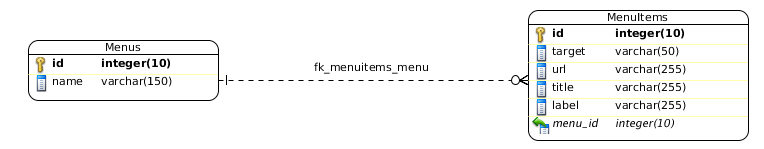
\includegraphics{erd.png}
\index{max\_items (fantastico.contrib.dynamic\_menu.menu\_controller.DynamicMenuController attribute)}

\begin{fulllineitems}
\phantomsection\label{features/components/dynamic_menu/dynamic_menu:fantastico.contrib.dynamic_menu.menu_controller.DynamicMenuController.max_items}\pysigline{\bfcode{max\_items}}
This property retrieves the maximum number of items allowed for a menu.

\end{fulllineitems}

\index{retrieve\_menu\_items() (fantastico.contrib.dynamic\_menu.menu\_controller.DynamicMenuController method)}

\begin{fulllineitems}
\phantomsection\label{features/components/dynamic_menu/dynamic_menu:fantastico.contrib.dynamic_menu.menu_controller.DynamicMenuController.retrieve_menu_items}\pysiglinewithargsret{\bfcode{retrieve\_menu\_items}}{\emph{*args}, \emph{**kwargs}}{}
This method is used to retrieve all items associated with a specified menu.
\begin{quote}\begin{description}
\item[{Parameters}] \leavevmode\begin{itemize}
\item {} 
\textbf{request} (\emph{HTTP request}) -- Http request being processed.

\item {} 
\textbf{menu\_id} (\emph{int}) -- Menu unique identifier we want to retrieve information for.

\end{itemize}

\item[{Returns}] \leavevmode
A JSON array containing all available menu items.

\item[{Raises {\hyperref[features/components/dynamic_menu/dynamic_menu:fantastico.contrib.dynamic_menu.menu_exceptions.FantasticoMenuNotFoundException]{fantastico.contrib.dynamic\_menu.menu\_exceptions.FantasticoMenuNotFoundException}}}] \leavevmode
Whenever the requested menu does not exist.

\end{description}\end{quote}

\end{fulllineitems}


\end{fulllineitems}

\index{FantasticoMenuNotFoundException (class in fantastico.contrib.dynamic\_menu.menu\_exceptions)}

\begin{fulllineitems}
\phantomsection\label{features/components/dynamic_menu/dynamic_menu:fantastico.contrib.dynamic_menu.menu_exceptions.FantasticoMenuNotFoundException}\pysiglinewithargsret{\strong{class }\code{fantastico.contrib.dynamic\_menu.menu\_exceptions.}\bfcode{FantasticoMenuNotFoundException}}{\emph{msg=None}, \emph{http\_code=400}}{}
This class defines a concrete fantastico menu not found exception raised whenever someone tries to access an inexistent
menu attributes.

\end{fulllineitems}



\subsection{Dynamic pages}
\label{features/components/dynamic_pages/dynamic_pages:dynamic-pages}\label{features/components/dynamic_pages/dynamic_pages::doc}
Most of the time, when a developer create a new web site or web application he follows the steps:
\begin{enumerate}
\item {} 
Create a set of templates (can be delegated to a web designer)

\item {} 
Create a new API or create a proxy API.

\item {} 
Create pages over the templates.

\end{enumerate}

Many web sites / applications have a minimal set of master templates and all web pages follow those templates. This kind of
approach keeps site consistency and decouple layouts from actual content. In \textbf{Fantastico}, it is extremely easy to work in this
manner thanks to \textbf{Dynamic pages} extension.

Dynamic pages divides pages into two main parts:
\begin{enumerate}
\item {} 
Page meta information (title, keywords, description, language)

\item {} 
Page model / content (markup, text keys or any other kind of information).

\end{enumerate}

Using dynamic pages you can easily add new web pages to your project without writing a single line of server side code.


\subsubsection{Integration}
\label{features/components/dynamic_pages/dynamic_pages:integration}\begin{enumerate}
\item {} 
Activate \textbf{Dynamic pages} extension.

\begin{Verbatim}[commandchars=\\\{\}]
fsdk activate\PYGZhy{}extension \PYGZhy{}\PYGZhy{}name dynamic\PYGZus{}pages \PYGZhy{}\PYGZhy{}comp\PYGZhy{}root \PYGZlt{}comp\PYGZus{}root\PYGZgt{}
\end{Verbatim}

\item {} 
Add new dynamic pages to your project using \textbf{\textless{}comp\_root\textgreater{}/sql/create\_data.sql}.

\begin{Verbatim}[commandchars=\\\{\}]
\PYG{k}{INSERT} \PYG{k}{INTO} \PYG{n}{pages}\PYG{p}{(}\PYG{n}{id}\PYG{p}{,} \PYG{n}{name}\PYG{p}{,} \PYG{n}{url}\PYG{p}{,} \PYG{k}{template}\PYG{p}{,} \PYG{n}{keywords}\PYG{p}{,} \PYG{n}{description}\PYG{p}{,} \PYG{n}{title}\PYG{p}{,} \PYG{k}{language}\PYG{p}{)}
\PYG{k}{VALUES}\PYG{p}{(}\PYG{l+m+mi}{1}\PYG{p}{,} \PYG{l+s+s1}{\PYGZsq{}/en/home\PYGZsq{}}\PYG{p}{,} \PYG{l+s+s1}{\PYGZsq{}/en/home\PYGZsq{}}\PYG{p}{,} \PYG{l+s+s1}{\PYGZsq{}/frontend/views/master.html\PYGZsq{}}\PYG{p}{,} \PYG{l+s+s1}{\PYGZsq{}keyword 1, ...\PYGZsq{}}\PYG{p}{,} \PYG{l+s+s1}{\PYGZsq{}Home page\PYGZsq{}}\PYG{p}{,} \PYG{l+s+s1}{\PYGZsq{}description\PYGZsq{}}\PYG{p}{,} \PYG{l+s+s1}{\PYGZsq{}en\PYGZhy{}US\PYGZsq{}}\PYG{p}{)}\PYG{p}{;}

\PYG{k}{INSERT} \PYG{k}{INTO} \PYG{n}{page\PYGZus{}models}\PYG{p}{(}\PYG{n}{page\PYGZus{}id}\PYG{p}{,} \PYG{n}{name}\PYG{p}{,} \PYG{n}{value}\PYG{p}{)}
\PYG{k}{VALUES}\PYG{p}{(}\PYG{l+m+mi}{1}\PYG{p}{,} \PYG{l+s+s1}{\PYGZsq{}article\PYGZus{}left\PYGZsq{}}\PYG{p}{,} \PYG{l+s+s1}{\PYGZsq{}\PYGZlt{}p class=\PYGZdq{}hello\PYGZus{}world\PYGZdq{}\PYGZgt{}Hello world.\PYGZlt{}/p\PYGZgt{}\PYGZsq{}}\PYG{p}{)}\PYG{p}{;}

\PYG{k}{INSERT} \PYG{k}{INTO} \PYG{n}{page\PYGZus{}models}\PYG{p}{(}\PYG{n}{page\PYGZus{}id}\PYG{p}{,} \PYG{n}{name}\PYG{p}{,} \PYG{n}{value}\PYG{p}{)}
\PYG{k}{VALUES}\PYG{p}{(}\PYG{l+m+mi}{1}\PYG{p}{,} \PYG{l+s+s1}{\PYGZsq{}article\PYGZus{}right\PYGZsq{}}\PYG{p}{,} \PYG{l+s+s1}{\PYGZsq{}\PYGZlt{}p class=\PYGZdq{}hello\PYGZus{}world\PYGZus{}right\PYGZdq{}\PYGZgt{}Hello world right.\PYGZlt{}/p\PYGZgt{}\PYGZsq{}}\PYG{p}{)}\PYG{p}{;}
\end{Verbatim}

\item {} 
Update your project database

\begin{Verbatim}[commandchars=\\\{\}]
fsdk syncdb \PYGZhy{}\PYGZhy{}db\PYGZhy{}command /usr/bin/mysql \PYGZhy{}\PYGZhy{}comp\PYGZhy{}root \PYGZlt{}comp\PYGZus{}root\PYGZgt{}
\end{Verbatim}

\item {} 
Create \textbf{master.html} template file under \textbf{\textless{}comp\_root\textgreater{}/frontend/views/}.

\begin{Verbatim}[commandchars=\\\{\}]
\PYG{c+cp}{\PYGZlt{}!DOCTYPE html\PYGZgt{}}

\PYG{n+nt}{\PYGZlt{}html} \PYG{n+na}{lang=}\PYG{l+s}{\PYGZdq{}\PYGZob{}\PYGZob{}page.language\PYGZcb{}\PYGZcb{}\PYGZdq{}}\PYG{n+nt}{\PYGZgt{}}
   \PYG{n+nt}{\PYGZlt{}head}\PYG{n+nt}{\PYGZgt{}}
      \PYG{n+nt}{\PYGZlt{}meta} \PYG{n+na}{http\PYGZhy{}equiv=}\PYG{l+s}{\PYGZdq{}Content\PYGZhy{}type\PYGZdq{}} \PYG{n+na}{content=}\PYG{l+s}{\PYGZdq{}text/html;charset=UTF\PYGZhy{}8\PYGZdq{}} \PYG{n+nt}{/\PYGZgt{}}
      \PYG{n+nt}{\PYGZlt{}meta} \PYG{n+na}{name=}\PYG{l+s}{\PYGZdq{}viewport\PYGZdq{}} \PYG{n+na}{content=}\PYG{l+s}{\PYGZdq{}width=device\PYGZhy{}width, initial\PYGZhy{}scale=1.0\PYGZdq{}}\PYG{n+nt}{\PYGZgt{}}
      \PYG{n+nt}{\PYGZlt{}meta} \PYG{n+na}{name=}\PYG{l+s}{\PYGZdq{}keywords\PYGZdq{}} \PYG{n+na}{content=}\PYG{l+s}{\PYGZdq{}\PYGZob{}\PYGZob{}page.keywords\PYGZcb{}\PYGZcb{}\PYGZdq{}} \PYG{n+nt}{/\PYGZgt{}}
      \PYG{n+nt}{\PYGZlt{}meta} \PYG{n+na}{name=}\PYG{l+s}{\PYGZdq{}description\PYGZdq{}} \PYG{n+na}{content=}\PYG{l+s}{\PYGZdq{}\PYGZob{}\PYGZob{}page.description\PYGZcb{}\PYGZcb{}\PYGZdq{}} \PYG{n+nt}{/\PYGZgt{}}

      \PYG{n+nt}{\PYGZlt{}title}\PYG{n+nt}{\PYGZgt{}}\PYGZob{}\PYGZob{}page.title\PYGZcb{}\PYGZcb{}\PYG{n+nt}{\PYGZlt{}/title\PYGZgt{}}
   \PYG{n+nt}{\PYGZlt{}/head\PYGZgt{}}

   \PYG{n+nt}{\PYGZlt{}body}\PYG{n+nt}{\PYGZgt{}}
      \PYG{n+nt}{\PYGZlt{}h1}\PYG{n+nt}{\PYGZgt{}}\PYGZob{}\PYGZob{}page.article\PYGZus{}left.value\PYGZcb{}\PYGZcb{}\PYG{n+nt}{\PYGZlt{}/h1\PYGZgt{}}

      \PYG{n+nt}{\PYGZlt{}h2}\PYG{n+nt}{\PYGZgt{}}\PYGZob{}\PYGZob{}page.article\PYGZus{}right.value\PYGZcb{}\PYGZcb{}\PYG{n+nt}{\PYGZlt{}/h2\PYGZgt{}}
   \PYG{n+nt}{\PYGZlt{}/body\PYGZgt{}}
 \PYG{n+nt}{\PYGZlt{}/html\PYGZgt{}}
\end{Verbatim}

\end{enumerate}

After you integrated \textbf{dynamic pages} extension into your project you can access
\href{http://localhost:12000/dynamic/test/default/page}{http://localhost:12000/dynamic/test/default/page} from a browser. You should see a very simple dynamic page rendered.


\subsubsection{Current limitations}
\label{features/components/dynamic_pages/dynamic_pages:current-limitations}
In the first version of this component (part of \textbf{Fantastico 0.4}) there are some known limitations:
\begin{itemize}
\item {} 
Create / Delete / Update / Bulk listing API are not provided. You can do this through create\_data.sql script.

\item {} 
There is no way to rewrite dynamic pages url so that they do not contain \emph{/dynamic} prefix.

\end{itemize}


\subsubsection{Technical summary}
\label{features/components/dynamic_pages/dynamic_pages:technical-summary}\index{PagesRouter (class in fantastico.contrib.dynamic\_pages.pages\_router)}

\begin{fulllineitems}
\phantomsection\label{features/components/dynamic_pages/dynamic_pages:fantastico.contrib.dynamic_pages.pages_router.PagesRouter}\pysiglinewithargsret{\strong{class }\code{fantastico.contrib.dynamic\_pages.pages\_router.}\bfcode{PagesRouter}}{\emph{settings\_facade}}{}
This class provides the API for managing dynamic pages. In addition, it creates the special route \textbf{/dynamic/\textless{}page\_url\textgreater{}}
used to access pages stored in the database. From dynamic pages module perspective, a web page is nothing more than a relation
between {\hyperref[features/components/dynamic_pages/dynamic_pages:fantastico.contrib.dynamic_pages.models.pages.DynamicPage]{\code{fantastico.contrib.dynamic\_pages.models.pages.DynamicPage}}} and
{\hyperref[features/components/dynamic_pages/dynamic_pages:fantastico.contrib.dynamic_pages.models.pages.DynamicPageModel]{\code{fantastico.contrib.dynamic\_pages.models.pages.DynamicPageModel}}}.

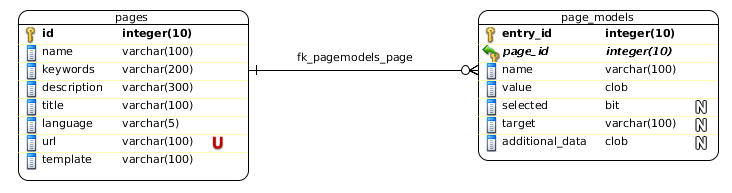
\includegraphics{erd1.png}

A typical template for dynamic pages might look like:

\begin{Verbatim}[commandchars=\\\{\}]
\PYG{c+cp}{\PYGZlt{}!DOCTYPE html\PYGZgt{}}

\PYG{n+nt}{\PYGZlt{}html} \PYG{n+na}{lang=}\PYG{l+s}{\PYGZdq{}\PYGZob{}\PYGZob{}page.language\PYGZcb{}\PYGZcb{}\PYGZdq{}}\PYG{n+nt}{\PYGZgt{}}
   \PYG{n+nt}{\PYGZlt{}head}\PYG{n+nt}{\PYGZgt{}}
      \PYG{n+nt}{\PYGZlt{}meta} \PYG{n+na}{http\PYGZhy{}equiv=}\PYG{l+s}{\PYGZdq{}Content\PYGZhy{}type\PYGZdq{}} \PYG{n+na}{content=}\PYG{l+s}{\PYGZdq{}text/html;charset=UTF\PYGZhy{}8\PYGZdq{}} \PYG{n+nt}{/\PYGZgt{}}
      \PYG{n+nt}{\PYGZlt{}meta} \PYG{n+na}{name=}\PYG{l+s}{\PYGZdq{}viewport\PYGZdq{}} \PYG{n+na}{content=}\PYG{l+s}{\PYGZdq{}width=device\PYGZhy{}width, initial\PYGZhy{}scale=1.0\PYGZdq{}}\PYG{n+nt}{\PYGZgt{}}
      \PYG{n+nt}{\PYGZlt{}meta} \PYG{n+na}{name=}\PYG{l+s}{\PYGZdq{}keywords\PYGZdq{}} \PYG{n+na}{content=}\PYG{l+s}{\PYGZdq{}\PYGZob{}\PYGZob{}page.keywords\PYGZcb{}\PYGZcb{}\PYGZdq{}} \PYG{n+nt}{/\PYGZgt{}}
      \PYG{n+nt}{\PYGZlt{}meta} \PYG{n+na}{name=}\PYG{l+s}{\PYGZdq{}description\PYGZdq{}} \PYG{n+na}{content=}\PYG{l+s}{\PYGZdq{}\PYGZob{}\PYGZob{}page.description\PYGZcb{}\PYGZcb{}\PYGZdq{}} \PYG{n+nt}{/\PYGZgt{}}

      \PYG{n+nt}{\PYGZlt{}link} \PYG{n+na}{href=}\PYG{l+s}{\PYGZdq{}/frontend/static/css/bootstrap\PYGZhy{}responsive.css\PYGZdq{}} \PYG{n+na}{rel=}\PYG{l+s}{\PYGZdq{}stylesheet\PYGZdq{}}\PYG{n+nt}{\PYGZgt{}}
      \PYG{n+nt}{\PYGZlt{}link} \PYG{n+na}{href=}\PYG{l+s}{\PYGZdq{}/frontend/static/css/forhidraulic.css\PYGZdq{}} \PYG{n+na}{rel=}\PYG{l+s}{\PYGZdq{}stylesheet\PYGZdq{}}\PYG{n+nt}{\PYGZgt{}}
      \PYG{n+nt}{\PYGZlt{}title}\PYG{n+nt}{\PYGZgt{}}\PYGZob{}\PYGZob{}page.title\PYGZcb{}\PYGZcb{}\PYG{n+nt}{\PYGZlt{}/title\PYGZgt{}}
   \PYG{n+nt}{\PYGZlt{}/head\PYGZgt{}}

   \PYG{n+nt}{\PYGZlt{}body}\PYG{n+nt}{\PYGZgt{}}
      \PYG{n+nt}{\PYGZlt{}h1}\PYG{n+nt}{\PYGZgt{}}\PYGZob{}\PYGZob{}page.article\PYGZus{}left.value\PYGZcb{}\PYGZcb{}\PYG{n+nt}{\PYGZlt{}/h1\PYGZgt{}}

      \PYG{n+nt}{\PYGZlt{}h2}\PYG{n+nt}{\PYGZgt{}}\PYGZob{}\PYGZob{}page.article\PYGZus{}right.value\PYGZcb{}\PYGZcb{}\PYG{n+nt}{\PYGZlt{}/h1\PYGZgt{}}
   \PYG{n+nt}{\PYGZlt{}/body\PYGZgt{}}
 \PYG{n+nt}{\PYGZlt{}/html\PYGZgt{}}
\end{Verbatim}
\index{serve\_dynamic\_page() (fantastico.contrib.dynamic\_pages.pages\_router.PagesRouter method)}

\begin{fulllineitems}
\phantomsection\label{features/components/dynamic_pages/dynamic_pages:fantastico.contrib.dynamic_pages.pages_router.PagesRouter.serve_dynamic_page}\pysiglinewithargsret{\bfcode{serve\_dynamic\_page}}{\emph{*args}, \emph{**kwargs}}{}
This method is used to route all /dynamic/... requests to database pages. It renders the configured template into
database binded to \code{fantastico.contrib.models.pages.DynamicPageModel} values.

\end{fulllineitems}


\end{fulllineitems}

\index{DynamicPage (class in fantastico.contrib.dynamic\_pages.models.pages)}

\begin{fulllineitems}
\phantomsection\label{features/components/dynamic_pages/dynamic_pages:fantastico.contrib.dynamic_pages.models.pages.DynamicPage}\pysiglinewithargsret{\strong{class }\code{fantastico.contrib.dynamic\_pages.models.pages.}\bfcode{DynamicPage}}{\emph{name=None}, \emph{url=None}, \emph{template=None}, \emph{keywords=None}, \emph{description=None}, \emph{title=None}, \emph{language='en'}}{}
This model holds meta information about dynamic pages. Below you can find all meta information for a dynamic page:
\begin{enumerate}
\item {} 
id (unique identifier for a dynamic page)

\item {} 
name

\item {} 
url

\item {} 
template

\item {} 
keywords

\item {} 
description

\item {} 
language

\end{enumerate}

In a template used for rendering dynamic pages, you can easily access page meta information:

\begin{Verbatim}[commandchars=\\\{\}]
\PYG{n+nt}{\PYGZlt{}p}\PYG{n+nt}{\PYGZgt{}}Id: \PYGZob{}\PYGZob{}page.id\PYGZcb{}\PYGZcb{}\PYG{n+nt}{\PYGZlt{}/p\PYGZgt{}}
\PYG{n+nt}{\PYGZlt{}p}\PYG{n+nt}{\PYGZgt{}}Name: \PYGZob{}\PYGZob{}page.name\PYGZcb{}\PYGZcb{}\PYG{n+nt}{\PYGZlt{}/p\PYGZgt{}}
\PYG{n+nt}{\PYGZlt{}p}\PYG{n+nt}{\PYGZgt{}}Url: \PYGZob{}\PYGZob{}page.url\PYGZcb{}\PYGZcb{}\PYG{n+nt}{\PYGZlt{}/p\PYGZgt{}}
\PYG{n+nt}{\PYGZlt{}p}\PYG{n+nt}{\PYGZgt{}}Template: \PYGZob{}\PYGZob{}page.template\PYGZcb{}\PYGZcb{}\PYG{n+nt}{\PYGZlt{}/p\PYGZgt{}}
\PYG{n+nt}{\PYGZlt{}p}\PYG{n+nt}{\PYGZgt{}}Keywords: \PYGZob{}\PYGZob{}page.keywords\PYGZcb{}\PYGZcb{}\PYG{n+nt}{\PYGZlt{}/p\PYGZgt{}}
\PYG{n+nt}{\PYGZlt{}p}\PYG{n+nt}{\PYGZgt{}}Description: \PYGZob{}\PYGZob{}page.description\PYGZcb{}\PYGZcb{}\PYG{n+nt}{\PYGZlt{}/p\PYGZgt{}}
\PYG{n+nt}{\PYGZlt{}p}\PYG{n+nt}{\PYGZgt{}}Language: \PYGZob{}\PYGZob{}page.language\PYGZcb{}\PYGZcb{}\PYG{n+nt}{\PYGZlt{}/p\PYGZgt{}}
\end{Verbatim}

Usually it does not make sense to display dynamic page unique identifier but you can do it if necessary.

\end{fulllineitems}

\index{DynamicPageModel (class in fantastico.contrib.dynamic\_pages.models.pages)}

\begin{fulllineitems}
\phantomsection\label{features/components/dynamic_pages/dynamic_pages:fantastico.contrib.dynamic_pages.models.pages.DynamicPageModel}\pysiglinewithargsret{\strong{class }\code{fantastico.contrib.dynamic\_pages.models.pages.}\bfcode{DynamicPageModel}}{\emph{page\_id=None}, \emph{name=None}, \emph{value=None}}{}
This class defines how page models looks like. A page model defines the actual content for en existing page.

\end{fulllineitems}



\subsection{Tracking codes}
\label{features/components/tracking_codes/tracking_codes:tracking-codes}\label{features/components/tracking_codes/tracking_codes::doc}
Every web application usually requires support for tracking visitors behavior. Most of the solutions can be easily integrated
into a website by adding a small javascript snippet into every page you want to track. Below you can find some popular tracking
solutions (free or commercial).


\subsubsection{Analytic solutions}
\label{features/components/tracking_codes/tracking_codes:analytic-solutions}
At the moment of writting this article, there are plenty of options available for web developers to track their
website performance:
\begin{enumerate}
\item {} 
\href{https://www.google.com/analytics/}{Google analytics} (probably the most popular solution).

\item {} 
\href{https://www.reinvigorate.net/}{Reinvigorate}.

\item {} 
\href{https://www.kissmetrics.com/}{KISSmetrics}.

\item {} 
\href{http://foxmetrics.com/}{FoxMetrics}.

\item {} 
\href{http://haveamint.com/}{Mint}.

\item {} 
\href{http://www.openwebanalytics.com/}{Open Web Analytics}.

\item {} 
\href{http://clicky.com/}{Clicky}.

\item {} 
\href{https://mixpanel.com/}{Mixpanel}.

\item {} 
\href{https://chartbeat.com/}{Chartbeat}.

\item {} 
\href{http://www.adobe.com/solutions/digital-analytics.html}{Adobe Web Analytics}.

\item {} 
\href{https://chartbeat.com/}{Chartbeat}.

\item {} 
\href{http://www.inspectlet.com/}{Inspectlet}.

\end{enumerate}

Of course there are many other solutions available out there. For more information about the above mentioned solution I recommend
you read the excellent \href{http://www.onextrapixel.com/2013/07/16/ten-best-alternatives-to-google-analytics/}{article}
posted by Aidan Huang.


\subsubsection{Integration}
\label{features/components/tracking_codes/tracking_codes:integration}
Follow the steps from this section in order to enable tracking in \textbf{Fantastico} projects:
\begin{enumerate}
\item {} 
Activate tracking extension:

\begin{Verbatim}[commandchars=\\\{\}]
fsdk activate\PYGZhy{}extension \PYGZhy{}\PYGZhy{}name tracking\PYGZus{}codes \PYGZhy{}\PYGZhy{}comp\PYGZhy{}root \PYGZlt{}comp\PYGZus{}root\PYGZgt{}
\end{Verbatim}

\item {} 
Add your tracking codes into database (easiest way is through {\hyperref[features/sdk/command_syncdb::doc]{\emph{Syncdb command}}})

\item {} 
Create a sql script similar to the one below and place it under \textbf{\textless{}comp\_root\textgreater{}/sql/create\_data.sql}:

\begin{Verbatim}[commandchars=\\\{\}]
\PYG{k}{INSERT} \PYG{k}{INTO} \PYG{n}{tracking\PYGZus{}codes}\PYG{p}{(}\PYG{n}{provider}\PYG{p}{,} \PYG{n}{script}\PYG{p}{)}
\PYG{k}{VALUES} \PYG{p}{(}\PYG{l+s+s1}{\PYGZsq{}Google Analytics\PYGZsq{}}\PYG{p}{,} \PYG{l+s+s1}{\PYGZsq{}}
\PYG{l+s+s1}{   \PYGZlt{}script type=\PYGZdq{}text/javascript\PYGZdq{}\PYGZgt{}}
\PYG{l+s+s1}{        var \PYGZus{}gaq = \PYGZus{}gaq \textbar{}\textbar{} [];}
\PYG{l+s+s1}{        \PYGZus{}gaq.push([\PYGZdq{}\PYGZus{}setAccount\PYGZdq{}, \PYGZdq{}UA\PYGZhy{}XXXXX\PYGZhy{}X\PYGZdq{}]);}
\PYG{l+s+s1}{        \PYGZus{}gaq.push([\PYGZdq{}\PYGZus{}trackPageview\PYGZdq{}]);}

\PYG{l+s+s1}{        (function() \PYGZob{}}
\PYG{l+s+s1}{          var ga = document.createElement(\PYGZdq{}script\PYGZdq{}); ga.type = \PYGZdq{}text/javascript\PYGZdq{}; ga.async = true;}
\PYG{l+s+s1}{          ga.src = (\PYGZdq{}https:\PYGZdq{} == document.location.protocol ? \PYGZdq{}https://ssl\PYGZdq{} : \PYGZdq{}http://www\PYGZdq{}) + \PYGZdq{}.google\PYGZhy{}analytics.com/ga.js\PYGZdq{};}
\PYG{l+s+s1}{          var s = document.getElementsByTagName(\PYGZdq{}script\PYGZdq{})[0]; s.parentNode.insertBefore(ga, s);}
\PYG{l+s+s1}{        \PYGZcb{})();}
\PYG{l+s+s1}{   \PYGZlt{}/script\PYGZgt{}\PYGZsq{}}\PYG{p}{)}\PYG{p}{;}
\end{Verbatim}

\item {} 
Update your project database

\begin{Verbatim}[commandchars=\\\{\}]
fsdk syncdb \PYGZhy{}\PYGZhy{}db\PYGZhy{}command /usr/bin/mysql \PYGZhy{}\PYGZhy{}comp\PYGZhy{}root \PYGZlt{}comp\PYGZus{}root\PYGZgt{}
\end{Verbatim}

\item {} 
Use tracking codes in your pages:

\begin{Verbatim}[commandchars=\\\{\}]
\PYGZob{}\PYGZpc{} component url=\PYGZdq{}/tracking\PYGZhy{}codes/ui/codes/\PYGZdq{} \PYGZpc{}\PYGZcb{}\PYGZob{}\PYGZpc{} endcomponent \PYGZpc{}\PYGZcb{}
\end{Verbatim}

\end{enumerate}

Tracking component is rendering all available codes from the database. In order to check all available tracking codes configured
in a \textbf{Fantastico} project visit \href{http://localhost:12000/tracking-codes/ui/codes/}{http://localhost:12000/tracking-codes/ui/codes/}. Once the page is loaded see page source.


\subsubsection{Current limitations}
\label{features/components/tracking_codes/tracking_codes:current-limitations}
In the first version of this component (part of \textbf{Fantastico 0.4}) there are some known limitations:
\begin{itemize}
\item {} 
No API provided for Create / Update / Delete operations.

\end{itemize}


\subsubsection{Technical summary}
\label{features/components/tracking_codes/tracking_codes:technical-summary}\index{TrackingController (class in fantastico.contrib.tracking\_codes.tracking\_controller)}

\begin{fulllineitems}
\phantomsection\label{features/components/tracking_codes/tracking_codes:fantastico.contrib.tracking_codes.tracking_controller.TrackingController}\pysiglinewithargsret{\strong{class }\code{fantastico.contrib.tracking\_codes.tracking\_controller.}\bfcode{TrackingController}}{\emph{settings\_facade}}{}~
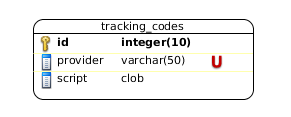
\includegraphics{erd2.png}

This class provides the tracking operations supported by \textbf{TrackingCodes} component.
\index{list\_codes() (fantastico.contrib.tracking\_codes.tracking\_controller.TrackingController method)}

\begin{fulllineitems}
\phantomsection\label{features/components/tracking_codes/tracking_codes:fantastico.contrib.tracking_codes.tracking_controller.TrackingController.list_codes}\pysiglinewithargsret{\bfcode{list\_codes}}{\emph{*args}, \emph{**kwargs}}{}
This method provides tracking codes listing logic. It list all available tracking codes from database.
\begin{quote}\begin{description}
\item[{Parameters}] \leavevmode
\textbf{request} (\code{webob.request.Request}) -- The current http request being processed. Read {\hyperref[features/request_response::doc]{\emph{Request lifecycle}}} for more information.

\item[{Returns}] \leavevmode
JSON list of available tracking codes. Can be empty if no tracking codes are defined.

\end{description}\end{quote}

\end{fulllineitems}

\index{list\_codes\_ui() (fantastico.contrib.tracking\_codes.tracking\_controller.TrackingController method)}

\begin{fulllineitems}
\phantomsection\label{features/components/tracking_codes/tracking_codes:fantastico.contrib.tracking_codes.tracking_controller.TrackingController.list_codes_ui}\pysiglinewithargsret{\bfcode{list\_codes\_ui}}{\emph{*args}, \emph{**kwargs}}{}
This method renders all available tracking codes.

\end{fulllineitems}


\end{fulllineitems}

\index{TrackingCode (class in fantastico.contrib.tracking\_codes.models.codes)}

\begin{fulllineitems}
\phantomsection\label{features/components/tracking_codes/tracking_codes:fantastico.contrib.tracking_codes.models.codes.TrackingCode}\pysiglinewithargsret{\strong{class }\code{fantastico.contrib.tracking\_codes.models.codes.}\bfcode{TrackingCode}}{\emph{provider}, \emph{script}}{}
This class provides the model for tracking codes. It maps \textbf{tracking\_codes} table to an object. In order to use this model
please read {\hyperref[features/mvc::doc]{\emph{Model View Controller}}}.

\end{fulllineitems}



\subsection{ROA Auto discovery}
\label{features/components/roa_discovery/roa_discovery::doc}\label{features/components/roa_discovery/roa_discovery:roa-auto-discovery}
REST relies on hypermedia and links in order to decouple clients from physical location of resources. In Fantastico,
we allow clients to introspect the platform in order to know which are the registered resources. Following some simple steps
you can enable autodiscovery of resources.


\subsubsection{Integration}
\label{features/components/roa_discovery/roa_discovery:integration}\begin{enumerate}
\item {} 
Activate \textbf{ROA Discovery} extension.

\begin{Verbatim}[commandchars=\\\{\}]
fsdk activate\PYGZhy{}extension \PYGZhy{}\PYGZhy{}name roa\PYGZus{}discovery \PYGZhy{}\PYGZhy{}comp\PYGZhy{}root \PYGZlt{}comp\PYGZus{}root\PYGZgt{}
\end{Verbatim}

\item {} 
Start your project

\item {} 
Access \href{http://localhost/roa/resources}{http://localhost/roa/resources}

\end{enumerate}

By default, \textbf{ROA Discovery} extension defines a sample resource (\textbf{Sample Resource}) which must be always present in your
discovery registry.


\subsubsection{Current limitations}
\label{features/components/roa_discovery/roa_discovery:current-limitations}\begin{itemize}
\item {} 
ROA discovery supports only application/json content type for responses.

\end{itemize}


\subsubsection{Technical summary}
\label{features/components/roa_discovery/roa_discovery:technical-summary}\index{RoaDiscoveryController (class in fantastico.contrib.roa\_discovery.discovery\_controller)}

\begin{fulllineitems}
\phantomsection\label{features/components/roa_discovery/roa_discovery:fantastico.contrib.roa_discovery.discovery_controller.RoaDiscoveryController}\pysiglinewithargsret{\strong{class }\code{fantastico.contrib.roa\_discovery.discovery\_controller.}\bfcode{RoaDiscoveryController}}{\emph{settings\_facade}, \emph{registry\_cls=None}}{}
This class provides the routes for introspecting Fantastico registered resources through ROA. It is extremely useful
to surf using your browser and to not be required to hardcode links in your code. Typically, you will want to code your
client side applications against resources name and you are going to use this controller to find the location of those
records.

By default, all ROA resources are mapped on \textbf{/api/} relative to current project root. You can easily change this behavior
by modifying the settings of your application ({\hyperref[get_started/settings:fantastico.settings.BasicSettings]{\code{fantastico.settings.BasicSettings}}} - property \textbf{roa\_api\_url})
\index{handle\_list\_resources\_options() (fantastico.contrib.roa\_discovery.discovery\_controller.RoaDiscoveryController method)}

\begin{fulllineitems}
\phantomsection\label{features/components/roa_discovery/roa_discovery:fantastico.contrib.roa_discovery.discovery_controller.RoaDiscoveryController.handle_list_resources_options}\pysiglinewithargsret{\bfcode{handle\_list\_resources\_options}}{\emph{*args}, \emph{**kwargs}}{}
This method handles all OPTIONS cors requests coming for resources registry listing.

\end{fulllineitems}

\index{list\_registered\_resources() (fantastico.contrib.roa\_discovery.discovery\_controller.RoaDiscoveryController method)}

\begin{fulllineitems}
\phantomsection\label{features/components/roa_discovery/roa_discovery:fantastico.contrib.roa_discovery.discovery_controller.RoaDiscoveryController.list_registered_resources}\pysiglinewithargsret{\bfcode{list\_registered\_resources}}{\emph{*args}, \emph{**kwargs}}{}
This method list all registered resources as well as a link to their entry point.

\begin{Verbatim}[commandchars=\\\{\}]
\PYG{c+c1}{// ROA api is mapped on a subdomain: roa.fantasticoproject.com}
\PYG{c+c1}{// listing is done by GET http://fantasticoproject.com/roa/resources HTTP/1.1}

\PYG{p}{\PYGZob{}}
    \PYG{l+s+s2}{\PYGZdq{}Person\PYGZdq{}}\PYG{o}{:} \PYG{p}{\PYGZob{}}\PYG{l+m+mf}{1.0} \PYG{o}{:} \PYG{l+s+s2}{\PYGZdq{}http://roa.fantasticoproject.com/1.0/persons\PYGZdq{}}\PYG{p}{,}
               \PYG{l+s+s2}{\PYGZdq{}latest\PYGZdq{}}\PYG{o}{:} \PYG{l+s+s2}{\PYGZdq{}http://roa.fantasticoproject.com/latest/persons\PYGZdq{}}\PYG{p}{\PYGZcb{}}\PYG{p}{,}
    \PYG{l+s+s2}{\PYGZdq{}Address\PYGZdq{}}\PYG{o}{:} \PYG{p}{\PYGZob{}}\PYG{l+m+mf}{1.0} \PYG{o}{:} \PYG{l+s+s2}{\PYGZdq{}http://roa.fantasticoproject.com/1.0/addresses\PYGZdq{}}\PYG{p}{,}
                \PYG{l+m+mf}{2.0} \PYG{o}{:} \PYG{l+s+s2}{\PYGZdq{}http://roa.fantasticoproject.com/2.0/addresses\PYGZdq{}}\PYG{p}{,}
                \PYG{l+s+s2}{\PYGZdq{}latest\PYGZdq{}}\PYG{o}{:} \PYG{l+s+s2}{\PYGZdq{}http://roa.fantasticoproject.com/latest/addresses\PYGZdq{}}\PYG{p}{\PYGZcb{}}
\PYG{p}{\PYGZcb{}}
\end{Verbatim}

\begin{Verbatim}[commandchars=\\\{\}]
\PYG{c+c1}{// ROA api is mapped on a relative path of the project: http://fantasticoproject.com/api/}
\PYG{c+c1}{// listing is done by GET http://fantasticoproject.com/roa/resources HTTP/1.1}

\PYG{p}{\PYGZob{}}
    \PYG{l+s+s2}{\PYGZdq{}Person\PYGZdq{}}\PYG{o}{:} \PYG{p}{\PYGZob{}}\PYG{l+m+mf}{1.0} \PYG{o}{:} \PYG{l+s+s2}{\PYGZdq{}http://fantasticoproject.com/api/1.0/persons\PYGZdq{}}\PYG{p}{,}
               \PYG{l+s+s2}{\PYGZdq{}latest\PYGZdq{}}\PYG{o}{:} \PYG{l+s+s2}{\PYGZdq{}http://roa.fantasticoproject.com/api/latest/persons\PYGZdq{}}\PYG{p}{\PYGZcb{}}\PYG{p}{,}
    \PYG{l+s+s2}{\PYGZdq{}Address\PYGZdq{}}\PYG{o}{:} \PYG{p}{\PYGZob{}}\PYG{l+m+mf}{1.0} \PYG{o}{:} \PYG{l+s+s2}{\PYGZdq{}http://roa.fantasticoproject.com/api/1.0/addresses\PYGZdq{}}\PYG{p}{,}
                \PYG{l+m+mf}{2.0} \PYG{o}{:} \PYG{l+s+s2}{\PYGZdq{}http://roa.fantasticoproject.com/api/2.0/addresses\PYGZdq{}}\PYG{p}{,}
                \PYG{l+s+s2}{\PYGZdq{}latest\PYGZdq{}}\PYG{o}{:} \PYG{l+s+s2}{\PYGZdq{}http://roa.fantasticoproject.com/api/latest/addresses\PYGZdq{}}\PYG{p}{\PYGZcb{}}
\PYG{p}{\PYGZcb{}}
\end{Verbatim}

\end{fulllineitems}


\end{fulllineitems}



\subsection{OAuth2 Identity Provider}
\label{features/components/oauth2/oauth2_idp/index::doc}\label{features/components/oauth2/oauth2_idp/index:oauth2-identity-provider}
This component provides the built in Fantastico identity provider which supports:
\begin{itemize}
\item {} 
Customizable login screen

\item {} 
API for users CRUD operations

\item {} 
API for persons.

\end{itemize}

You can read more about this on {\hyperref[features/oauth2/idp::doc]{\emph{OAUTH2 Fantastico IDP}}}.


\subsubsection{Integration}
\label{features/components/oauth2/oauth2_idp/index:integration}
In order to use OAuth2 identity provider into your project follow the steps below:
\begin{enumerate}
\item {} 
Activate \textbf{OAuth2 IDP} extension.

\begin{Verbatim}[commandchars=\\\{\}]
fsdk activate\PYGZhy{}extension \PYGZhy{}\PYGZhy{}name oauth2\PYGZus{}idp \PYGZhy{}\PYGZhy{}comp\PYGZhy{}root \PYGZlt{}comp\PYGZus{}root\PYGZgt{}
\end{Verbatim}

\item {} 
Synchronize your database with latest changes.

\begin{Verbatim}[commandchars=\\\{\}]
fsdk syncdb \PYGZhy{}\PYGZhy{}db\PYGZhy{}command /usr/bin/mysql \PYGZhy{}\PYGZhy{}comp\PYGZhy{}root \PYGZlt{}comp\PYGZus{}root\PYGZgt{}
\end{Verbatim}

\item {} 
Run development server.

\item {} 
Visit \href{http://localhost:12000/oauth/authorize?response\_type=token\&state=xyz\&error\_format=hash\&client\_id=11111111-1111-1111-1111-111111111111\&scope=user.profile.read\&redirect\_uri=/oauth/idp/ui/cb}{http://localhost:12000/oauth/authorize?response\_type=token\&state=xyz\&error\_format=hash\&client\_id=11111111-1111-1111-1111-111111111111\&scope=user.profile.read\&redirect\_uri=/oauth/idp/ui/cb}

\item {} 
Log with \href{mailto:admin@fantastico.com}{admin@fantastico.com} / 1234567890

\item {} 
You should see a success html page which displays your access token.

\end{enumerate}


\chapter{Changes}
\label{changes:changes}\label{changes::doc}

\section{Feedback}
\label{changes:feedback}
I really hope you enjoy using Fantastico framework as much as we love developing it. Your feedback is highly appreciated
so do not hesitate to get in touch with us (for support, feature requests, suggestions, or everything else is on your mind):
\href{https://docs.google.com/forms/d/1tKBopU3lfDB\_w8F4h7Rl1Rn4uydAJq-nha09L\_ptJck/edit?usp=sharing}{Provide feedback}


\section{Versions}
\label{changes:versions}\begin{itemize}
\item {} 
v0.7.0 (stable)
\begin{itemize}
\item {} 
Added support for cross origin requests on ROA resources registry (/roa/resources).

\item {} 
Added support for exception serialized responses CORS compatible requests.

\item {} 
Add CORS decorator for enabling CORS headers on custom controller routes.

\item {} 
Add support for headers appended to each response (support for global CORS configurable headers).

\item {} 
Fix cors for ROA fetch individual item.

\item {} 
Fix @RequiredScopes attribute for MVC controllers (now it automatically validates the security context before invoking underline method).

\item {} 
Improve implicit grant handler so that it supports non redirect responses.

\end{itemize}

\item {} 
v0.6.0 (\href{https://docs.google.com/forms/d/1tKBopU3lfDB\_w8F4h7Rl1Rn4uydAJq-nha09L\_ptJck/edit?usp=sharing}{Provide feedback})
\begin{itemize}
\item {} 
Added implicit grant type implementation.

\item {} 
Added security support for endpoints / controllers.

\item {} 
Added Fantastico identity provider.

\item {} 
Fix a bug in ROA APIs routes mapping.

\item {} 
Added support for MVC Controllers into custom packages (not residing in components root folder).

\item {} 
Added ROA resources dependent on user (integrated with OAuth2 access tokens).

\item {} 
Added ROA resources OAuth2 authorization.

\item {} 
!!!!! ROA ResourceValidator base class now adds two more methods for formatting resources and is backward incompatible with Fantastico version 0.5.1.

\item {} 
!!!!! ROA ResourceValidator validate method has changed signature and is backware incompatible with Fantastico version 0.5.1.

\end{itemize}

\item {} 
v0.5.1 (\href{https://docs.google.com/forms/d/1tKBopU3lfDB\_w8F4h7Rl1Rn4uydAJq-nha09L\_ptJck/edit?usp=sharing}{Provide feedback})
\begin{itemize}
\item {} 
Add a tutorial for creating TODO application based on ROA. (\href{http://rcosnita.github.io/fantastico/html/how\_to/todo/index.html}{http://rcosnita.github.io/fantastico/html/how\_to/todo/index.html})

\item {} 
Deployed TODO web application on a public accessible server. (\href{http://todo.fantastico.scrum-expert.ro/frontend/ui/index}{http://todo.fantastico.scrum-expert.ro/frontend/ui/index})

\item {} 
Fix roa discovery component fsdk syncdb bug on subsequent runs.

\item {} 
Fix roa api cors support.

\end{itemize}

\item {} 
v0.5.0 (\href{https://docs.google.com/forms/d/1tKBopU3lfDB\_w8F4h7Rl1Rn4uydAJq-nha09L\_ptJck/edit?usp=sharing}{Provide feedback})
\begin{itemize}
\item {} 
Added specification for auto generated API for resources.

\item {} 
Added OAUTH2 draft implementation details for Fantastico.

\item {} 
Added Identity Provider draft specification.

\item {} 
Added REST API Standard for ROA (Resource Oriented Architecture).

\item {} 
Added REST filter parser implementation using fast ll grammar for ROA (Resource Oriented Architecture).

\item {} 
Added auto generated APIs for resources (Resource Oriented Architecture).

\item {} 
Improved routing loaders so that multiple methods can serve separate http verbs of a route.

\item {} 
Added support for multiple routes mapped on the same controller.

\item {} 
Fixed a bug in MySql connections pool (not recycling correctly after a long idle period).

\item {} 
I changed thread local MySql connection strategy to request based.

\end{itemize}

\item {} \begin{description}
\item[{v0.4.1 (\href{https://docs.google.com/forms/d/1tKBopU3lfDB\_w8F4h7Rl1Rn4uydAJq-nha09L\_ptJck/edit?usp=sharing}{Provide feedback})}] \leavevmode\begin{itemize}
\item {} 
Fix a bug into analytics component sample data insert.

\item {} 
Fix a bug into component rendering for no json responses coming for given url.

\end{itemize}

\end{description}

\item {} \begin{description}
\item[{v0.4.0 (\href{https://docs.google.com/forms/d/1tKBopU3lfDB\_w8F4h7Rl1Rn4uydAJq-nha09L\_ptJck/edit?usp=sharing}{Provide feedback})}] \leavevmode\begin{itemize}
\item {} 
Fantastico SDK commands display official link to command documentation.

\item {} 
Fantastico SDK syncdb command.

\item {} 
Standard detection of database tables module setup / data insert created.

\item {} 
Multiple tracking codes extension integrated into fantastico contrib.

\item {} 
Dynamic pages extension integrated into fantastico contrib.

\item {} 
Direct feedback channel integrated into documentation (\href{https://docs.google.com/forms/d/1tKBopU3lfDB\_w8F4h7Rl1Rn4uydAJq-nha09L\_ptJck/edit?usp=sharing}{Provide feedback})

\end{itemize}

\end{description}

\item {} \begin{description}
\item[{v0.3.0}] \leavevmode\begin{itemize}
\item {} 
Fantastico SDK core is available.

\item {} 
Fantastico SDK activate-extension command is available.

\item {} 
Samples of how to activate extensions for an existing project are provided.

\end{itemize}

\end{description}

\item {} \begin{description}
\item[{v0.2.2}] \leavevmode\begin{itemize}
\item {} 
Update dynamic menu activation documentation.

\item {} 
Fix a serious bug in engine management and too many sql connections opened.

\item {} 
Fix a bug in db session close when an unexpected error occurs when opening the connection.

\item {} 
Add extensive unit tests for db session management.

\end{itemize}

\end{description}

\item {} \begin{description}
\item[{v0.2.1}] \leavevmode\begin{itemize}
\item {} 
Fix packaging of pypi package. Now it is usable and contains rendering package as well as contrib package.

\end{itemize}

\end{description}

\item {} \begin{description}
\item[{v0.2.0}] \leavevmode\begin{itemize}
\item {} 
Framework documentation is tracked using Google Analytics

\item {} 
Component reusage is done using \{\% component \%\} tag.

\item {} 
Dynamic menu pluggable component can be used out of the box.

\item {} 
MVC documentation improvements.

\item {} 
Fix a bug in DB session management cache when configuration was changed at runtime.

\end{itemize}

\end{description}

\item {} \begin{description}
\item[{v0.1.2}] \leavevmode\begin{itemize}
\item {} 
Nginx config file now also maps www.\textless{}vhost\_name\textgreater{}

\item {} 
Redirect support from controllers

\item {} 
Setup fantastico framework script does not override deployment files anymore

\end{itemize}

\end{description}

\item {} \begin{description}
\item[{v0.1.1}] \leavevmode\begin{itemize}
\item {} 
Favicon route handling.

\item {} 
Deployment scripts error handling and root folder execution (rather than execution only for deployment subfolder).

\item {} 
MVC how to article was changed to use get\_records\_paged instead of all\_paged method (it used to be a bug in documentation).

\item {} 
DB Session manager was changed from one singleton connection to connection / request.

\item {} 
FantasticoIntegrationTestCase now has a property that holds os environment variable name for setting up Fantastico active config.

\end{itemize}

\end{description}

\item {} \begin{description}
\item[{v0.1.0}] \leavevmode\begin{itemize}
\item {} 
Built in router that can be easily extended.

\item {} 
WebOb Request / Response architecture.

\item {} 
Request context support for accessing various attributes (current language, current user and other attributes).

\item {} 
Multiple project profiles support.

\item {} 
Database simple configuration for multiple environments.

\item {} 
Model - View - Controller support.

\item {} 
Automatic model facade generator.

\item {} 
Model facade injection into Controllers.

\item {} 
Templating engine support for views (jinja2).

\item {} 
Documentation generator for pdf / html / epub formats.

\item {} 
Automatic framework packaging and deployment.

\item {} 
Helper scripts for creating projects based on Fantastico.

\item {} 
Easy rollout script for running Fantastico projects behind nginx.

\item {} 
Rollout scenarios for deploying Fantastico projects on Amazon (AWS).

\item {} 
How to sections for creating new projects and components using Fantastico.

\end{itemize}

\end{description}

\end{itemize}


\chapter{Provide feedback}
\label{index:provide-feedback}
\href{https://docs.google.com/forms/d/1tKBopU3lfDB\_w8F4h7Rl1Rn4uydAJq-nha09L\_ptJck/edit?usp=sharing}{Provide feedback}


\chapter{Build status}
\label{index:build-status}
If you want to see the current build status of the project visit \href{http://jenkins.scrum-expert.ro:8080/job/fantastico-framework/badge/icon/}{Build status}.


\chapter{License}
\label{index:license}
Copyright 2013 Cosnita Radu Viorel

Permission is hereby granted, free of charge, to any person obtaining a copy of this software and associated
documentation files (the ``Software''), to deal in the Software without restriction, including without limitation
the rights to use, copy, modify, merge, publish, distribute, sublicense, and/or sell copies of the Software,
and to permit persons to whom the Software is furnished to do so, subject to the following conditions:

The above copyright notice and this permission notice shall be included in all copies or substantial portions of the Software.

THE SOFTWARE IS PROVIDED ``AS IS'', WITHOUT WARRANTY OF ANY KIND, EXPRESS OR IMPLIED, INCLUDING BUT NOT LIMITED TO THE
WARRANTIES OF MERCHANTABILITY, FITNESS FOR A PARTICULAR PURPOSE AND NONINFRINGEMENT. IN NO EVENT SHALL THE AUTHORS OR
COPYRIGHT HOLDERS BE LIABLE FOR ANY CLAIM, DAMAGES OR OTHER LIABILITY, WHETHER IN AN ACTION OF CONTRACT, TORT OR OTHERWISE,
ARISING FROM, OUT OF OR IN CONNECTION WITH THE SOFTWARE OR THE USE OR OTHER DEALINGS IN THE SOFTWARE.



\renewcommand{\indexname}{Index}
\printindex
\end{document}
